%%
%% Copyright 2007, 2008, 2009 Elsevier Ltd
%%
%% This file is part of the 'Elsarticle Bundle'.
%% ---------------------------------------------
%%
%% It may be distributed under the conditions of the LaTeX Project Public
%% License, either version 1.2 of this license or (at your option) any
%% later version.  The latest version of this license is in
%%    http://www.latex-project.org/lppl.txt
%% and version 1.2 or later is part of all distributions of LaTeX
%% version 1999/12/01 or later.
%%
%% The list of all files belonging to the 'Elsarticle Bundle' is
%% given in the file `manifest.txt'.
%%

%% Template article for Elsevier's document class `elsarticle'
%% with numbered style bibliographic references
%% SP 2008/03/01
%%
%%
%%
%% $Id: elsarticle-template-num.tex 4 2009-10-24 08:22:58Z rishi $
%%
%%
%%% DHW single column 
% \documentclass[preprint,12pt]{elsarticle}

%% Use the option review to obtain double line spacing
%% \documentclass[preprint,review,12pt]{elsarticle}

%% Use the options 1p,twocolumn; 3p; 3p,twocolumn; 5p; or 5p,twocolumn
%% for a journal layout:
%% \documentclass[final,1p,times]{elsarticle}
%%  71 pages with following line: DHW  
%% \documentclass[final,1p,times,twocolumn]{elsarticle}
%% \documentclass[final,3p,times]{elsarticle}
%% \documentclass[final,3p,times,twocolumn]{elsarticle}
%% \documentclass[final,5p,times]{elsarticle}
\documentclass[final,5p,times,longtitle,twocolumn]{elsarticle}

%% if you use PostScript figures in your article
%% use the graphics package for simple commands
%% \usepackage{graphics}
%% or use the graphicx package for more complicated commands
\usepackage{graphicx}
%% or use the epsfig package if you prefer to use the old commands
%% \usepackage{epsfig}
\usepackage{verbatim}
%% The amssymb package provides various useful mathematical symbols
\usepackage{amssymb}
\usepackage{float}
\usepackage{url}
\newcommand{\greeksym}[1]{{\usefont{U}{psy}{m}{n}#1}}
\newcommand{\umu}{\mbox{\greeksym{m}}}
\newcommand{\udelta}{\mbox{\greeksym{d}}}
\newcommand{\uDelta}{\mbox{\greeksym{D}}}
\newcommand{\uPi}{\mbox{\greeksym{P}}}
\renewcommand{\vec}[1]{\mathbf{#1}}
\renewcommand*{\thefootnote}{\fnsymbol{footnote}}
\newcommand{\Gfour}{{\scshape Geant4}}

%% For MT section
\newcommand{\gclass}[1]{\texttt{#1}}
\newcommand{\gmethod}[1]{\texttt{#1}}
\newcommand{\userclass}[1]{\texttt{#1}}
\newcommand{\gkeyword}[1]{\texttt{#1}}
\newcommand{\thread}{\texttt{\_\_thread} }
%% The amsthm package provides extended theorem environments
%% \usepackage{amsthm}

%% The lineno packages adds line numbers. Start line numbering with
%% \begin{linenumbers}, end it with \end{linenumbers}. Or switch it on
%% for the whole article with \linenumbers after \end{frontmatter}.
% \usepackage{lineno}

%% natbib.sty is loaded by default. However, natbib options can be
%% provided with \biboptions{...} command. Following options are
%% valid:

%%   round  -  round parentheses are used (default)
%%   square -  square brackets are used   [option]
%%   curly  -  curly braces are used      {option}
%%   angle  -  angle brackets are used    <option>
%%   semicolon  -  multiple citations separated by semi-colon
%%   colon  - same as semicolon, an earlier confusion
%%   comma  -  separated by comma
%%   numbers-  selects numerical citations
%%   super  -  numerical citations as superscripts
%%   sort   -  sorts multiple citations according to order in ref. list
%%   sort&compress   -  like sort, but also compresses numerical citations
%%   compress - compresses without sorting
%%
%% \biboptions{comma,round}

% \biboptions{}

\journal{Nuclear Instruments and Methods in Physics Research A}

\begin{document}

\begin{frontmatter}

%% Title, authors and addresses

%% use the tnoteref command within \title for footnotes;
%% use the tnotetext command for the associated footnote;
%% use the fnref command within \author or \address for footnotes;
%% use the fntext command for the associated footnote;
%% use the corref command within \author for corresponding author footnotes;
%% use the cortext command for the associated footnote;
%% use the ead command for the email address,
%% and the form \ead[url] for the home page:
%%
% \title{Recent Developments in Geant4\tnoteref{label1}}
% \tnotetext[label1]{Note here}
%% \author{Name\corref{cor1}\fnref{label2}}
%% \ead{email address}
%% \ead[url]{home page}
%% \fntext[label2]{}
%% \cortext[cor1]{}
%% \address{Address\fnref{label3}}
%% \fntext[label3]{}

% \title{Recent Developments in Geant4 \vspace{0.75cm}}
\title{Recent Developments in Geant4}

%% use optional labels to link authors explicitly to addresses:
%% Get numerical superscripts
% \def\theaffn{\arabic{affn}}

\author[a,b]{J. Allison}
\address[a]{Geant4 Associates International Ltd., 9 Royd Terrace, Hebden Bridge HX7 7BT, United Kingdom}
\address[b]{The University of Manchester, School of Physics and Astronomy, Manchester M13 9PL, United Kingdom}

\author[c,a]{K. Amako}
\address[c]{KEK, 1-1 Oho, Tsukuba, Ibaraki 305-0801, Japan}

\author[d]{J. Apostolakis}
\address[d]{CERN, 1211 Gen\'{e}ve 23, Switzerland}

\author[e]{P. Arce}
\address[e]{CIEMAT, Medical Applications Unit, Avenida Complutense 40, 28040 Madrid, Spain}

\author[f]{M. Asai}
\address[f]{SLAC National Accelerator Laboratory, 2575 Sand Hill Road, Menlo Park, CA 94025, USA}

\author[g]{T. Aso}
\address[g]{National Institute of Technology, Toyama College, 1-2 Ebie Neriya, Imizu, Toyama 9330293, Japan}

\author[h]{E.~Bagli}
\address[h]{INFN Sezione di Ferrara, Via Saragat 1, 44122 Ferrara, Italy}

\author[i]{A. Bagulya}
\address[i]{Lebedev Physical Institute, Leninskii Pr. 53, Moscow 119991, Russia}

\author[j]{S. Banerjee}
\address[j]{Fermi National Accelerator Laboratory, P.O. Box 500, Batavia, IL 60510, USA}

\author[k]{G. Barrand}
\address[k]{IN2P3/LAL, Universite Paris-Sud, Orsay, France}

\author[l]{B.R.~Beck}
\address[l]{Lawrence Livermore National Laboratory, 7000 East Avenue, Livermore, CA 94550, USA}

\author[m]{A.G.~Bogdanov}
\address[m]{National Research Nuclear University (Moscow Engineering Physics Institute), 
            Kashirskoe shosse 31, Moscow 115409, Russia}

\author[n]{D. Brandt}
\address[n]{SSW Trading, Am Knick 4, Oststeinbek, Germany}

\author[o]{J.M.C. Brown}
\address[o]{Queen's University Belfast, School of Mathematics and Physics, University Road, Belfast, Northern Ireland BT7 1NN, United Kingdom}

\author[d]{H.~Burkhardt}

\author[j]{Ph. Canal}

\author[p]{D.~Cano-Ott} 
\address[p]{CIEMAT, Centro de Investigaciones Energ\'{e}ticas Medioambientales y Tecn\'{o}logicas, Avenida Complutense 40, 28040 Madrid, Spain} 

\author[q]{S. Chauvie}
\address[q]{Sante Croce e Carle Hospital, Via Coppino 26, I-12100, Cuneo, Italy}

\author[r]{K. Cho}
\address[r]{National Institute of Supercomputing and Networking, Korea Institute of Science and Technology Information, 245 Daehak-ro, Yuseonggu, Daejeon 34141, Korea}

\author[s]{G.A.P.~Cirrone}
\address[s]{Istituto Nazionale di Fisica Nucleare, Laboratori Nazionali del Sud,
            Via Santa Sofia 62, 95123 Catania, Italy}

\author[t]{G. Cooperman}
\address[t]{Northeastern University, College of Computer and Information Science, 202-WVH, Boston, MA 02481, USA}

\author[u]{M.A. Cort\'{e}s-Giraldo}
\address[u]{Universidad de Sevilla, Departamento de F\'{i}sica At\'{o}mica, Molecular y Nuclear, Apdo. 1065, E-41080, Sevilla, Spain} 

\author[d]{G. Cosmo}

\author[s]{G. Cuttone} 

\author[x]{G. Depaola}
\address[x]{Universidad Nacional de C\'ordoba - FaMAF, Medina Allende s/n., C\'ordoba, Argentina}

\author[bt]{L.~Desorgher}
\address[bt]{Institut de Radiophysique, Rue du Grand-Pr\'{e} 1 CH-1007, Lausanne, Switzerland}

\author[t]{X. Dong}

\author[f]{A.~Dotti}

\author[j]{V.D.~Elvira}

\author[d]{G. Folger}

\author[v]{Z. Francis}
\address[v]{Universite Saint Joseph, Department de Physique, Beirut, Lebanon} 

\author[w]{A. Galoyan}
\address[w]{Veksler and Baldin Laboratory of High Energy Physics,
            Joint Institute for Nuclear Research,
            Joliot-Curie 6, Dubna, Moscow region, Russia, 141980}

\author[k]{L. Garnier\fnref{1}}
\fntext[1]{current affiliation: OSUR/CNRS Observatoire des 
           Sciences de l'Univers de Rennes, Universit{\'e} de Rennes1, Campus de
           Beaulieu, 35042 Rennes Cedex, France}

\author[d]{M. Gayer}

\author[j]{K.L.~Genser}

\author[i,d]{V.M.~Grichine}

\author[y,z]{S.~Guatelli}
\address[y]{University of Wollongong, Centre for Medical Radiation Physics, 
            Northfields Avenue, Wollongong, NSW 2522, Australia}
\address[z]{Illawarra Health and Medical Research Institute, Northfields Avenue,
            Wollongong, NSW 2522, Australia}
 
\author[aa]{P.~Gu\`{e}ye}
\address[aa]{Hampton University, Physics Department, 100 E. Queen Street,
             Hampton, VA 23668, USA}

\author[ab]{P. Gumplinger}
\address[ab]{TRIUMF, 4004 Wesbrook Mall, Vancouver, BC V6T 2A3, Canada}

\author[ac]{A.S. Howard}
\address[ac]{ETH Z{\"u}rich, IPP, Otto-Stern-Weg 5, 8093 Z{\"u}rich, Switzerland}

\author[ad]{I. H\v{r}ivn\'{a}\v{c}ov\'{a}}
\address[ad]{Institut de Physique Nucl\'{e}aire, Universit\'{e} Paris-Sud,
             CNRS-IN2P3, 15 rue Georges, Clemenceau, 91406 Orsay, Cedex, France}

\author[r,ae]{S.~Hwang}
\address[ae]{University of Science and Technology, 217 Gajeong-ro Yuseonggu,
             Daejeon, Korea}

\author[af,ag]{S. Incerti}
\address[af]{CNRS-IN2P3, CENBG, UMR 5797, F-33170 Gradignan, France}
\address[ag]{Universit\'{e} Bordeaux, CENBG, UMR 5797, F-33170 Gradignan, France}

\author[ah,a,d]{A.~Ivanchenko}
\address[ah]{Centre d'Etudes Nucl\'{e}aires de Bordeaux Gradignan,
             19 Chemin du Solarium, 33175 Gradignan, France}

\author[d,a,ai]{V.N.~Ivanchenko}
\address[ai]{Ecoanalytica, Moscow 119899, Russia}

\author[ab]{F.W. Jones}

\author[j]{S.Y.~Jun}

\author[aj,ak]{P.~Kaitaniemi\fnref{2}}
\address[aj]{CEA/Saclay, Centre de Saclay, Irfu/SPhN, F-91191 Gif-sur-Yvette, France}
\address[ak]{Helsinki Institute of Physics, P.O. Box 64, Gustaf H{\"a}llstr{\"o}m 
            Street 2, FI-00014, University of Helsinki, Finland}
\fntext[2]{current affiliation: Pandia Oy, Hiomotie 10, 5th floor, 00380 Helsinki, Finland}

\author[al,am]{N. Karakatsanis\fnref{3}}
\address[al]{National Technical University of Athens, School of Electrical and
             Computer Engineering, 9 Iroon Polytechniou St., Zografos, Athens 15780,
             Greece}
\address[am]{Johns Hopkins University, School of Medicine, 601 N. Caroline St.,
             Baltimore, MD 21287, USA}  
\fntext[3]{current affiliation: Translational and
               Molecular Imaging Institute, Icahn School of Medicine at Mt. Sinai,
               1470 Madison Avenue, New York, NY 10029, USA}

\author[an]{M. {\"K}aramitrosi}
\address[an]{Notre Dame University, Notre Dame Radiation Laboratory, Notre Dame,
            IN 46556, USA}

\author[f]{M.~Kelsey}

\author[ao]{A.~Kimura}
\address[ao]{Ashikaga Institute of Technology, Omae 268-1, Ashikaga, Tochigi 326-8558,
             Japan}

\author[f]{T.~Koi}

\author[ap]{H.~Kurashige}
\address[ap]{Kobe University, 1-1 Rokkodai, Nada, Kobe 657, Japan}

\author[d]{A. Lechner}

\author[aq]{S.B. Lee}
\address[aq]{National Cancer Center, 323 Insa-ro, Ilsandong-gu, Goyang-Si,
             Gyeonggi-do 10408, Korea}

\author[ar,as]{F.~Longo}
\address[ar]{University of Trieste, Department of Physics, Via Valerio 2, 34127 Trieste, Italy}
\address[as]{INFN, Trieste, Via Valerio 2, 34127 Trieste, Italy}

% \author{M. {\"M}aire\fnref{at,a}}
\author[at,a]{M. Maire}
\address[at]{IN2P3/LAPP, 74941 Annecy-le-vieux, France}

\author[au]{D. Mancusi}
\address[au]{CEA, Centre de Saclay, DEN/DANS/DM2S/SERMA/LTSD, 91191 Gif-sur-Yvette, CEDEX, France}

\author[av]{A.~Mantero}
\address[av]{SWHARD srl, Via greto di Cornigliano 6R, Genova, Italy}

\author[p]{E.~Mendoza}

\author[aw]{B.~Morgan}
\address[aw]{University of Warwick, Department of Physics, Gibbet Hill Road,
             Coventry CV4 7AL, United Kingdom}

\author[c]{K.~Murakami}

\author[d]{T. Nikitina}

\author[s]{L. Pandola}

\author[d]{P. Paprocki\fnref{4}}
\fntext[4]{current affiliation: Elarcos, Kabacki Dukt 8/32,
           02-798 Warsaw, Poland}

\author[f]{J.~Perl}

\author[ax]{I. Petrovi\'{c}} 
\address[ax]{University of Belgrade, Vin\v{c}a Institute of Nuclear Sciences,
             P.O. Box 522, 11001, Belgrade, Serbia}

\author[ay]{M.G. Pia}
\address[ay]{INFN Sezione di Genova, Via Dodecaneso 33, 16136 Genova, Italy}

\author[d]{W.~Pokorski}

\author[u]{J.M.~Quesada}

\author[az]{M.~Raine}
\address[az]{CEA, DAM, DIF, F-91297, Arpajon, France}

\author[ba,bb]{M.A. Reis}
\address[ba]{C2TN, Instituto Superior T\'{e}cnico,
             Universidade de Lisboa,
             Campus Tecnol\'{o}gico e Nuclear,
             EN10 km139.7, 2685-066 Bobadela LRS, Portugal}
\address[bb]{IEQUALTECS, Lda, Rua Dr. Francisco S\'{a} Carneiro, 36, 2500-065
             S. Greg\'{o}rio CLD, Portugal}

\author[d]{A.~Ribon}

\author[ax]{A. Risti\'{c} Fira}

\author[s]{F. Romano}

\author[s,bc]{G.~Russo}
\address[bc]{IBFM-CNR, Contrada Pietrapollastra, Pisciotta, 90020 Cefalu, Italy}

\author[bd,be]{G. Santin}
\address[bd]{European Space Agency/ESTEC, Keplerlaan 1, 2201AZ, Noordwijk, The Nehterlands}
\address[be]{RHEA System BV, Jonckerweg 18, 2201DZ, Noordwijk, The Nehterlands}

\author[c,bf]{T.~Sasaki}
\address[bf]{SOKENDAI, 1560-35, Hayama, Kanagawa 240-0193, Japan}

\author[bg]{D. Sawkey}
\address[bg]{Varian Medical Systems, 3120 Hansen Way, Palo Alto, CA 94304, USA}

\author[aq]{J.I.~Shin\fnref{5}}
\fntext[5]{current affiliation: Korea Institute of Radiological
           and Medical Sciences, 75 Nowon-ro, Nowon-gu, Seoul, 139-706 Korea}

\author[bh]{I.I.~Strakovsky}
\address[bh]{The George Washington University, Department of Physics, Washington, DC 20052, USA}

\author[ba]{A.~Taborda}

\author[bi]{S. Tanaka}
\address[bi]{Ritsumeikan University, College of Information Science and Engineering, 
             Noji-higashi 1-1-1, Kusatsu, Shiga 525-8577, Japan}

\author[bj]{B. Tom{\'e}}
\address[bj]{LIP-Lisboa/IST, Av. Elias Garcia, 14-1, 1000-149, Lisboa, Portugal}

\author[bk]{T. Toshito}
\address[bk]{Nagoya Proton Therapy Center, 1-1-1 Hirate-cho, Kita-ku, Nagoya 462-8508, Japan}

\author[bl,bm]{H.N.~Tran}
\address[bl]{Ton Duc Thang University, Division of Nuclear Physics, 19 Nguyen Huu Tho Street,
             Tan Phong Ward, District 7, Ho Chi Minh City, Vietnam}
\address[bm]{Ton Duc Thang University, Faculty of Applied Sciences, 19 Nguyen Huu Tho Street,
             Tan Phong Ward, District 7, Ho Chi Minh City, Vietnam}

\author[bn]{P.R.~Truscott}
\address[bn]{Kallisto Consultancy Ltd., Farnborough, Hampshire, GU14 9AJ, United Kingdom}

\author[a]{L. Urban}

\author[bo]{V. Uzhinsky}
\address[bo]{Laboratory of Information Technologies,
             Joint Institute for Nuclear Research,
             Joliot-Curie 6, Dubna, Moscow region, Russia, 141980} 

\author[l]{J.M. Verbeke}

\author[bp]{M.~Verderi}
\address[bp]{Universit{\'e} Paris-Saclay, Laboratoire Leprince-Ringuet, Ecole Polytechnique,
             CNRS/IN2P3, 91128, Palaiseau, France}

\author[bq]{B.L. Wendt}
\address[bq]{Idaho State University, 921 South 8th Avenue, Pocatello, ID 83209, USA}

\author[j]{H.~Wenzel}

\author[f]{D.H.~Wright}

\author[l]{D.M.~Wright}

\author[br]{T.~Yamashita}
\address[br]{Hyogo Ion Beam Medical Center, Tatsuno, Japan}

\author[j]{J.~Yarba}

\author[bs,a]{H. Yoshida}
\address[bs]{Naruto University of Education, Takashima, Naruto-shi, Japan}


\begin{abstract}
\Gfour{} is a software toolkit for the simulation of the passage of particles
through matter.  It is used by a large number of experiments and projects in a
variety of application domains, including high energy physics, astrophysics and
space science, medical physics and radiation protection.  Over the past several
years, major changes have been made to the toolkit in order to accommodate the
needs of these user communities, and to efficiently exploit the growth of 
computing power made available by advances in technology.  The adaptation of 
\Gfour{} to multithreading, advances in physics, detector modeling and 
visualization, extensions to the toolkit, including biasing and reverse Monte
Carlo, and tools for physics and release validation are discussed here.
\end{abstract}

\begin{keyword}
high energy physics \sep nuclear physics \sep radiation \sep simulation \sep computing 

%% MSC codes here, in the form: \MSC code \sep code
%% or \MSC[2008] code \sep code (2000 is the default)

\end{keyword}

\end{frontmatter}

%%
%% Start line numbering here if you want
%%
% DHW \begin{linenumbers}

%% main text
\section{The Evolution of \Gfour{}}

%%%%%%%%%%%%%%%%%%%%%%%%%%%%%%%%%%%%%%%%%%%%%%%%%%%
% evolution.tex
%%%%%%%%%%%%%%%%%%%%%%%%%%%%%%%%%%%%%%%%%%%%%%%%%%%
\label{sec:evolution}

A major trend in modern experimental science is the increased reliance upon
simulation to design complex detectors and interpret the data they produce.
Indeed, simulation has become mission-critical in fields such as high energy
physics and space science.  Another trend is the rapid increase in computing
power due to faster processors, multi-core architectures and distributed 
computing.  At the same time, advances in memory technology have not kept
pace and the amount of memory available per CPU cycle has decreased.  These 
trends have led to a re-examination of some of the basic assumptions of 
simulation computing, and to the evolution of the \Gfour{} simulation toolkit.

The toolkit approach has enabled \Gfour{} to serve a wide variety of user 
communities and to change as users' needs change.  Now sixteen years since its
initial public release, \Gfour{} continues to be the simulation engine of choice 
for high energy physics experiments at the LHC.  ESA and NASA have used and 
continue to use \Gfour{} in the design of spacecraft and the estimation of 
radiation doses received by astronauts and electronic components.  It is also 
used extensively in medical physics applications such as particle beam therapy, 
microdosimetry and radioprotection.  The basic extensibility of the toolkit 
has facilitated its expansion into new user domains, such as biochemistry,
material science and non-destructive scanning.   

Common to nearly all these domains, but especially true for high energy physics,
is the demand for increasingly detailed geometries and more sophisticated 
physical models.  This in turn drives the need for more CPU cycles, and the 
relative decrease of memory drives the need for more efficient memory 
management.  

It became clear that \Gfour{} could meet these challenges by adopting the 
multithreading approach and exploiting the multi-core architectures that have 
now become commonplace.  While significant effort went into the implementation 
of multithreading, the object-oriented design of the toolkit made the changes 
much less intrusive than might have been expected.  Section 2 of this document
will discuss the details and performance of this implementation.

The remainder of the document will deal with other improvements in the toolkit
since the last \Gfour{} general paper \cite{bib:generalpaper2}.
Section 3 covers improvements in kernel functionalities.  Among these are
new tracking and scoring capabilities, improved geometry models which have 
resulted in faster, more versatile experimental representations, and improved 
visualization techniques which provide users with more powerful ways to view 
them.  Section 4 provides updates in electromagnetic and hadronic physics 
modeling with discussions of recently introduced models, improvements in 
existing models and physics lists, and results from comparisons to data.
Extensions of the toolkit, including a new generic biasing framework, reverse
Monte Carlo, native analysis capability, and improved examples, are covered 
in Section 5.  Section 6 describes the extensive improvements in testing and
validation.  Modern web interfaces and standard testing tools have made it 
easier for users and developers alike to evaluate the performance of \Gfour{}.
The adoption of modern build tools addressed the need for flexible 
configuration and support on various computing platforms, as well as the 
ever-increasing number of data files needed by physics models.
This document concludes in Section 7 with a brief summary of \Gfour{} progress
and a discussion of prospects for the next decade.

\textit{A primer of terms.}
A number of terms within \Gfour{} have meanings which differ somewhat from 
general usage.  Although defined elsewhere \cite{bib:generalpaper2}, they are
reviewed here for convenience.

A \textit{track} is a snapshot of a particle at a particular point along its
path.  Instances of the class \gclass{G4Track} contain the particle's current
energy, momentum, position, time and so on, as well as its mass, charge,
lifetime and other quantities.

A \textit{trajectory} is a collection of track snapshots along the particle
path.

A \textit{step} consists of the two endpoints which bound the fundamental
propagation unit in space or time.  The length between the two points is chosen
by a combination of transportation and physics processes, and may be limited
to a fixed size by the user in cases where small step lengths are desired.  An
instance of \gclass{G4Step} stores the change in track properties between the 
two endpoints.

\textit{Process} has two meanings in \Gfour{}.  In the usual computer science 
sense, it refers to an instance of an application which is being executed.  This
is the meaning assumed in the discussion of multithreading.  In all 
other discussions the narrow \Gfour{} meaning is assumed: a class implementing a
physical or navigational interaction.  A \Gfour{} process is categorized by when 
the interaction occurs, either at the end of the step (\gclass{PostStep}) or 
during the step (\gclass{AlongStep}).

An \textit{event} consists of the decay or interaction of a primary particle and
a target, and all subsequent interactions, produced particles and four-vectors.
\gclass{G4Event} objects contain primary vertices and particles, and may contain
hits, digitizations and trajectories.

A \textit{run} consists of a series of events.



\section{Multithreading}

% Authors: Makoto Asai, Andrea Dotti, John Apostolakis, Gene Cooperman, Gabriele Cosmo
%%%%%%%%%%%%%%%%%%%%%%%%%%%%%%%%%%%%%%%%%%%%%%%%%%%
% multithreading.tex
%%%%%%%%%%%%%%%%%%%%%%%%%%%%%%%%%%%%%%%%%%%%%%%%%%%
\label{sec:multithreading}

\subsection{\textbf{The transition to multithreading}}
The emergence of multi-core and many-core processors has been a well-established
trend in the chip-making industry during the past decade.  While this paradigm 
guarantees the continued increase of CPU performance, it requires some 
adaptation of existing code in order to better utilize these architectures.  In
typical \Gfour{} simulations the most widespread approach for exploiting 
parallelism is job or process parallelism.  This is the spawning of multiple 
copies of the same process, and is being used in large-scale production by HEP 
experiments to exploit today's hardware.  However a key challenge for this 
approach is that the amount of random access memory (RAM) required scales 
linearly with the number of processes.  As the number of cores increases beyond
8 or 16, the amount of RAM may become a limiting factor unless a robust solution
for the sharing of memory between processes (or an alternative method) can be 
adopted in production systems.

This is especially true for co-processor technologies in which a high core count
is associated with a relatively limited amount of RAM, as in the Intel Xeon Phi 
co-processor card model 7120P, which hosts 16GB of RAM for 61 physical cores.

In \Gfour{} an alternative solution was developed, in which multithreaded 
applications share a substantial part of their data between threads in order to
significantly reduce the memory footprint.  In this design the memory savings 
are obtained by sharing among all the threads the key data which are constant 
during simulation: the geometry description and the tables used by 
electromagnetic physics processes \cite{MT:xdong}.  Threads are otherwise 
independent.

In this implementation each thread is responsible for simulating one or more
full events, thus implementing event-level parallelism.  Measurements 
demonstrate that this approach scales well with the number of threads.  Almost
linear scaling was obtained from two up to 60 physical cores, the maximum available
on shared memory systems that were available for benchmarking.  Additional 
throughput gains of about 20-30\% were obtained by using hyperthreading.

\begin{figure}[htb]
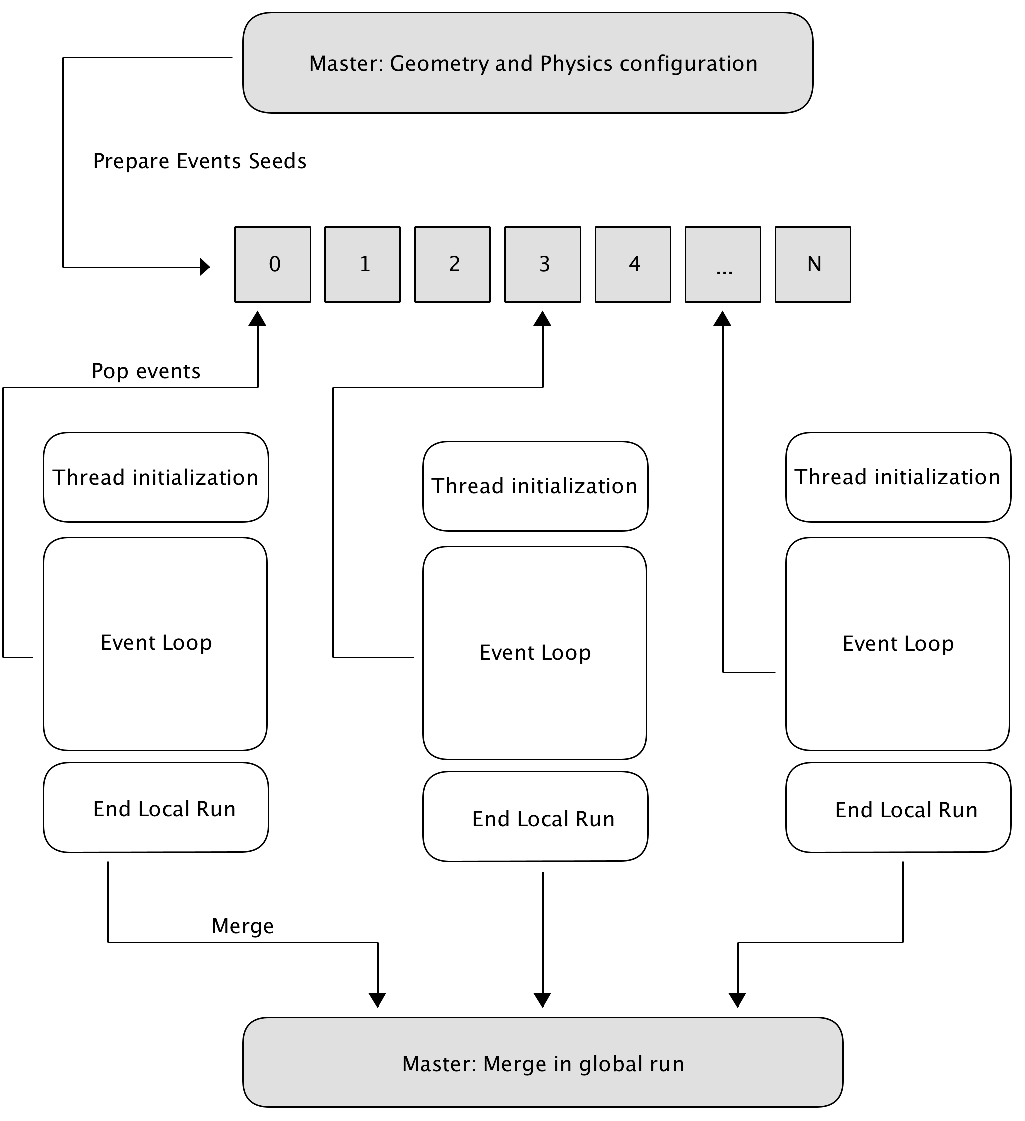
\includegraphics[width=0.47\textwidth]{figures/MTSchema.pdf}
\caption{Simplified description of a \Gfour{} multithreaded application: the
        {\it master} thread prepares geometry and physics setups for the simulation,
        and the {\it worker} threads compete for the next (group of) events to be
        simulated; otherwise they are independent.}
\label{fig:MTschema}
\end{figure}

\begin{figure}[htb]
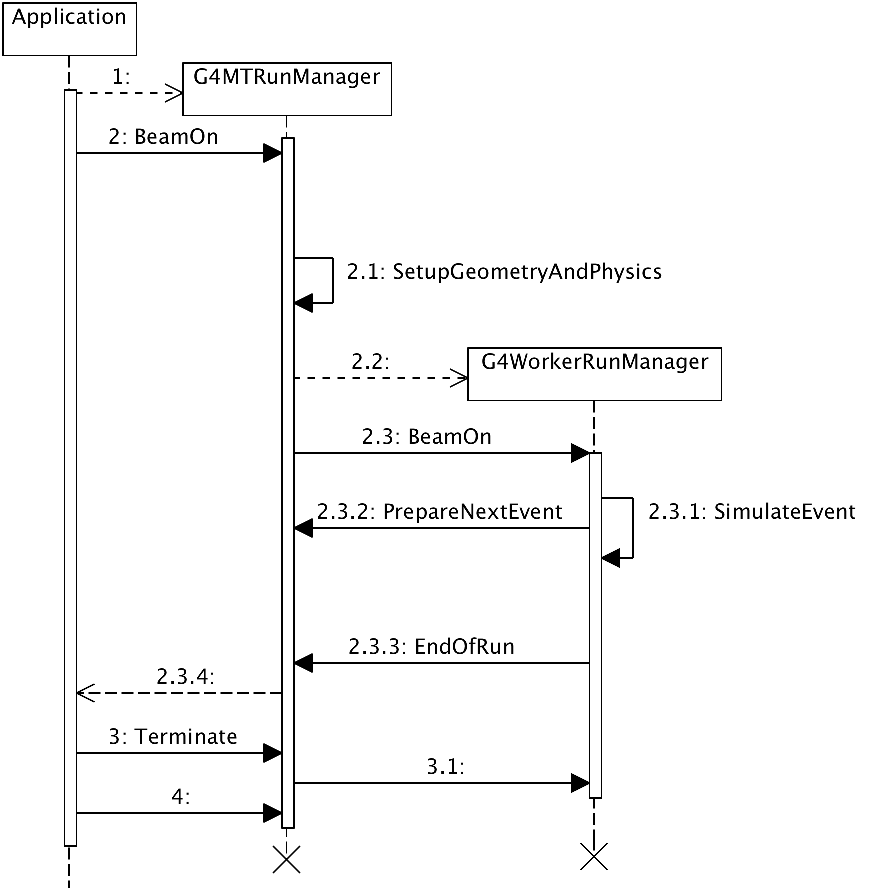
\includegraphics[width=0.45\textwidth]{figures/MTSimpleLife2A.pdf}
\caption{Sequence diagram of a multithreaded \Gfour{} application. The 
         application instantiates one \gclass{G4MTRunManager}.  When the 
         first run is started one or more worker threads are spawned. 
         The simulation in each worker thread is controlled by the local
         \gclass{G4WorkerRunManager}.}
\label{fig:MTlifecycle}
\end{figure}

\begin{figure}[htb]
    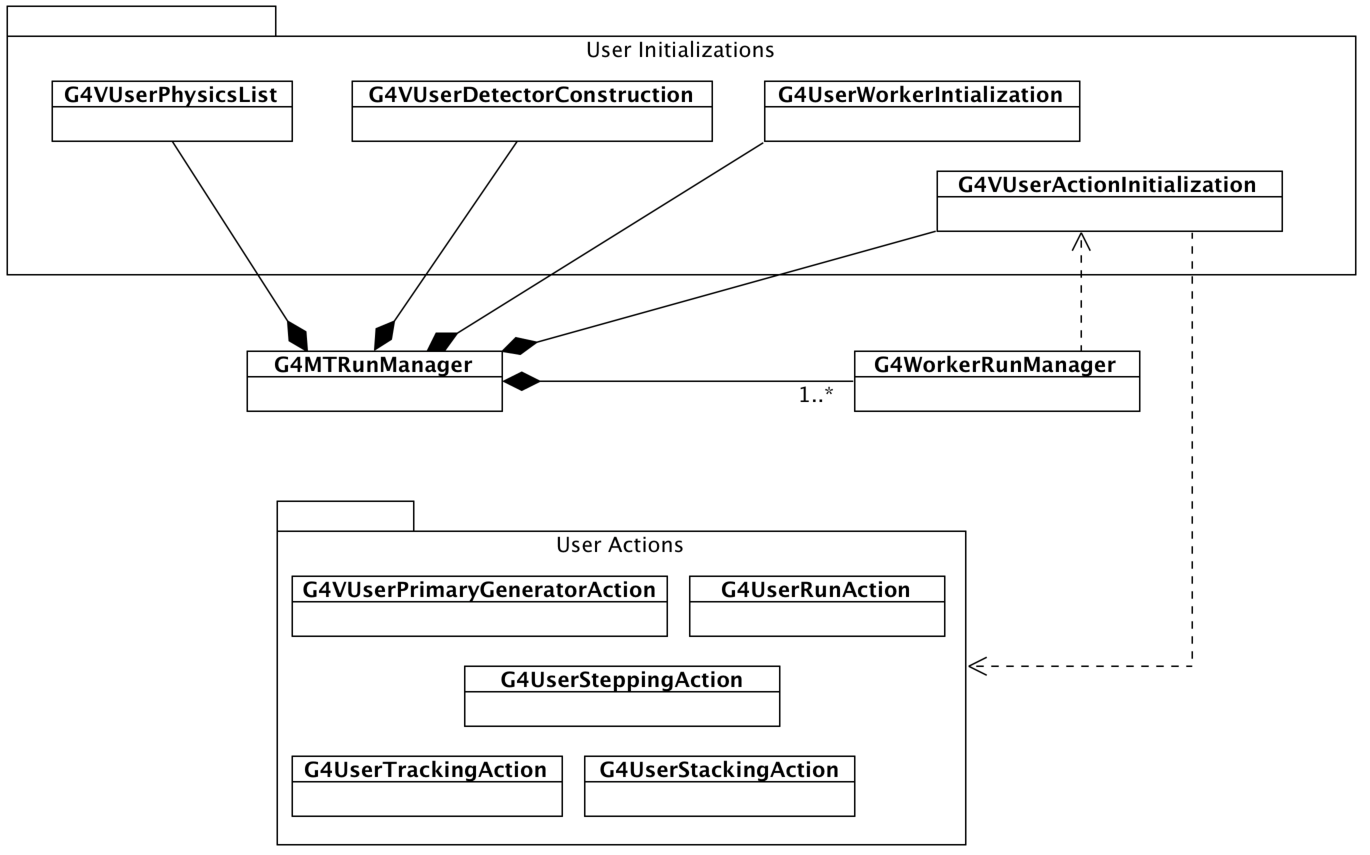
\includegraphics[width=0.45\textwidth]{figures/MTGeneralPaper2.pdf}
  \caption{Class diagram of the main user interfaces \cite{MT:TDG}. 
           User initializations (e.g. geometry and physics list) are shared
           among threads and are assigned to the single instance of
           \gclass{G4MTRunManager}, while user actions are created for each 
           thread (via \gclass{G4VUserActionInitialization}) and assigned to 
           the thread-private \gclass{G4WorkerRunManager}.}
  \label{fig:design}
\end{figure}

\subsection{\textbf{General Design}}
As a Monte Carlo simulation toolkit, \Gfour{} profits from improved throughput
via parallelism derived from the independence of modeled events and their 
computation.  Until \Gfour{} version 10.0, parallelization was obtained with a
simple distribution of inputs: each computation unit (e.g. a core of a node in a
cluster) ran a separate instance of \Gfour{} that was given a separate set of 
input events and associated random number seeds.

Given a computer with {\it k} cores, the design goal of multithreaded \Gfour{} was
to replace {\it k} independent instances of a \Gfour{} process with a single, 
equivalent process with {\it k} threads using the many-core machine in a 
memory-efficient, scalable manner.  The corresponding methodology involved 
transforming the code for thread safety and memory footprint reduction
\cite{MT:SNA2013}.  A simplified schema of the multithreading model used is 
shown in Figure~\ref{fig:MTschema}.  

Before the parallel section of the simulation begins, the geometry and physics
configurations are prepared and the random number engine is initialized in order
to generate a random sequence of uniformly distributed numbers.  This guarantees
reproducibility (see below).  Threads compete for the next group of events to be 
simulated, requesting one or more seeds from the shared seeds queue.  Output 
produced by the threads can be reduced at the end of the run.  If the application
uses the command-line scoring mechanism or histograms from the \Gfour{} analysis 
package, output from these is reduced automatically.  User-defined 
\gclass{G4Run} instances can be merged if they implement a \gmethod{Merge} method.

The multithreading option is based on a {\it master-worker} model in which one 
control sequence (the {\it master}) is responsible for initializing the geometry
and physics, and for spawning and controlling {\it worker} threads.  Workers are 
responsible for the simulation of one or more events.  The sequence diagram of a
\Gfour{} application is shown in Figure~\ref{fig:MTlifecycle} where the main 
interfaces (\gclass{G4MTRunManager} and \gclass{G4WorkerRunManager}) and their 
interactions are shown.

A \Gfour{} application is defined by the use of an instance of the 
\gclass{G4Run\allowbreak{}Manager} class or of a user-defined class derived from
it.  This class defines the main interaction with the user: it provides 
interfaces to define the {\it user initializations} (e.g. geometry and physics 
definitions) and the {\it user actions} that permit interaction with the 
simulation kernel and retrieve output information.  In particular,
\gclass{G4Run\allowbreak{}Manager} provides the interface to start the 
simulation of a run, which is a collection of events.  For multithreaded 
applications a derived class \gclass{G4MTRun\allowbreak{}Manager} is used 
that allows the number of worker threads to be specified.  Shared objects, such
as the geometry and physics list, are registered by the user to the instance of
this class, while the creation of user actions is the responsibility of a new 
class \gclass{G4VUserActionInitialization}.  When a new run is requested it is 
the responsibility of \gclass{G4MTRunManager} to start and configure worker 
threads.  Each thread owns an instance of \gclass{G4WorkerRunManager} and it 
shares only the user initialization classes, while it owns a private copy of the
user action classes.  Workers continue to request events from the master until 
there are no more events left in the current run.  At the end of the run the 
results collected by threads can be merged in the global run.

The communication between master and workers was implemented with a simple 
barrier mechanism to synchronize threads, and with the exchange of simple 
threading messages which currently may be one of:
\begin{itemize} 
\item {\it workers start new run} (instruct worker threads to begin the event
      loop),
\item {\it workers terminate} (instruct workers that the job has concluded, 
      workers should terminate and exit), or
\item {\it wait for workers ready} (master thread is waiting for one or more 
      workers to terminate current event loop, idle workers wait for further 
      messages).
\end{itemize}
User-defined code can be implemented by specializing key interfaces of certain
classes.  In particular, the \gclass{G4UserWorker\allowbreak{}Initialization} 
class defines the threading model and determines how threads are configured.  
The main \Gfour{} classes relevant to a multithreaded application are depicted
in Figure~\ref{fig:design}.  All interfaces are also available in sequential 
mode so that user code for a simulation application can be run both in 
multithreaded or sequential \Gfour{} with minimal changes.

\subsection{\textbf{Results}}
The physics and CPU performance of \Gfour{} were measured by comparing the
sequential version of the code to a multithreaded equivalent.  The results which
follow were obtained with a patched version of \Gfour{} Version 10.0, and 
%10.0.-ref0X
focus on high energy physics applications.  This domain was chosen because its 
complex physics requirements cover the most important use-cases for \Gfour{} 
users:
\begin{itemize}
\item high and low energy electromagnetic physics,
\item high and low energy hadronic physics, 
\item tracking in many-volume geometries and
\item tracking in electromagnetic fields.
\end{itemize}
In the near future regular testing will be extended to other user domains such
as medicine and space science.

So far, two applications have been adapted to multithreading.  The first is a 
test suite (Simplified Calorimeter) based on a simple geometry setup which allows
the study of all types of primary particle species over a very wide energy
range\cite{MT:6154433}.  The most interesting particles are electrons and hadrons
at high energy because they exercise the majority of physics models used in HEP
simulations of full showers.  Optional analyses can be performed on the 
predictions of the simulation in order to study typical HEP quantities.  These 
include both integral quantities like the total energy deposit, and detailed 
aspects of showers such as the number and type of interactions, and the energy 
spectra of produced secondaries.

The second application uses the \Gfour{} GDML interface\cite{MT:GDML} to
read a realistic geometry description of the CMS experiment at the LHC 
\cite{MT:collaboration2008cms}.  No analysis of simulated data is performed, but
a large set of materials and geometrical shapes is tested.  This application has
been used to test physics performance on different hardware setups, including 
Intel Xeon, ARM, PowerPC and Intel Atom processors, and Intel Xeon Phi 
co-processors.

% \begin{figure}[htb]
%     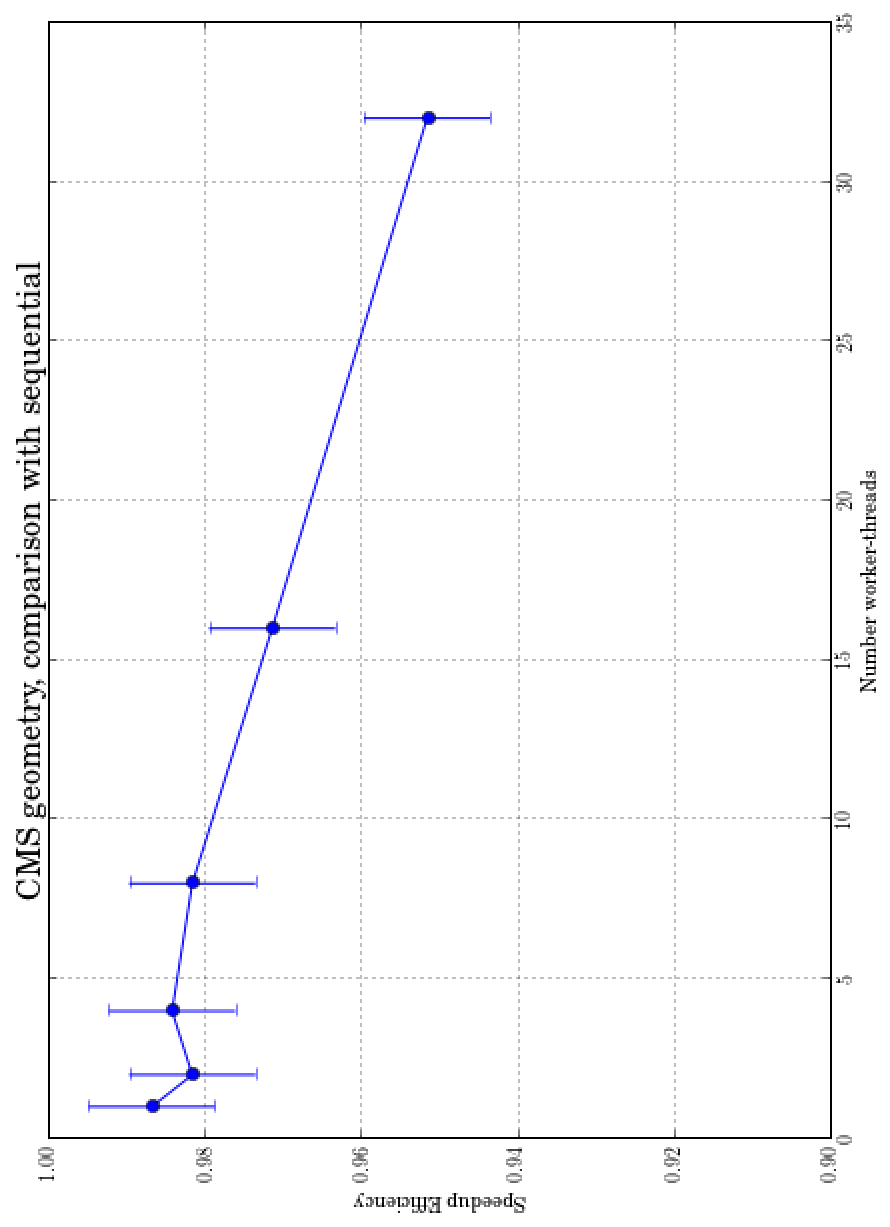
\includegraphics[width=0.35\textwidth, angle=-90]{figures/MTCPU.pdf}
%   \caption{Speedup efficiency (ratio of throughput of a run with {\it k} threads 
%            to the throughput of the sequential version), as a function of the 
%            number of threads, for the CMS simulation on an AMD-equipped server 
%            (Opteron Processor 6128 running at 2.40Hz, 4 CPU sockets x 8 cores). 
%            The multithreading overhead for one thread is only 1\%, while the 
%            efficiency is greater than 95\% for up to the maximum number of 
%            threads.} 
%   \label{fig:MTcpu}
% \end{figure}

\subsubsection{Physics equivalence to sequential}
It is of course required that the physics calculations are the same in both the
multithreaded and sequential versions.  Two tests were developed to verify this.
The first performs a statistical comparison of physics quantities simulated with
the Simplified Calorimeter testing suite.  Typical experimental observables 
(response, resolution and shower shapes) are compared between multithreaded
and sequential versions of the same application.  The resulting distributions 
were confirmed to be statistically equivalent. In this test the RNG engine seeds
used in the sequential and multithreading applications were not the same.

A more stringent test compares, event by event, the history of the random number
generator (RNG) engine.  To guarantee that reproducibility is independent of the 
number of threads and of the order in which events are simulated, each thread 
owns a separate instance of the RNG engine, and its status is re-initialized 
before the simulation of each event with a separate pre-defined seed.  The test
consists of two steps: a multithreaded application is run and the RNG engine 
seed recorded at the beginning of each event, together with the status of the 
engine at the end of the event simulation.  The same application is then run in
sequential mode, with the RNG engine re-initialized for each event with the seed
from the first run.  The engine status at the end of each event should be the 
same in the sequential and multithreaded versions.  It was verified that this 
occurs for 100\% of the cases, except for the test using the radioactive decay 
module.  This remaining discrepancy is being investigated, but it is thought to 
be due to violations of strict reproducibility - the independence of the 
results for a particular \Gfour{} event from the history of previous events.  
Extensive checking of the strong reproducibility of \Gfour{} physics models and 
physics lists has significantly reduced the incidence of such issues.  Strong
reproducibility of all classes used in a \Gfour{} application is an important 
requirement for providing consistent results in multithreaded runs, as results 
must not depend on the number of workers, or on the assignment of events to 
workers.
\begin{figure}[htb]
    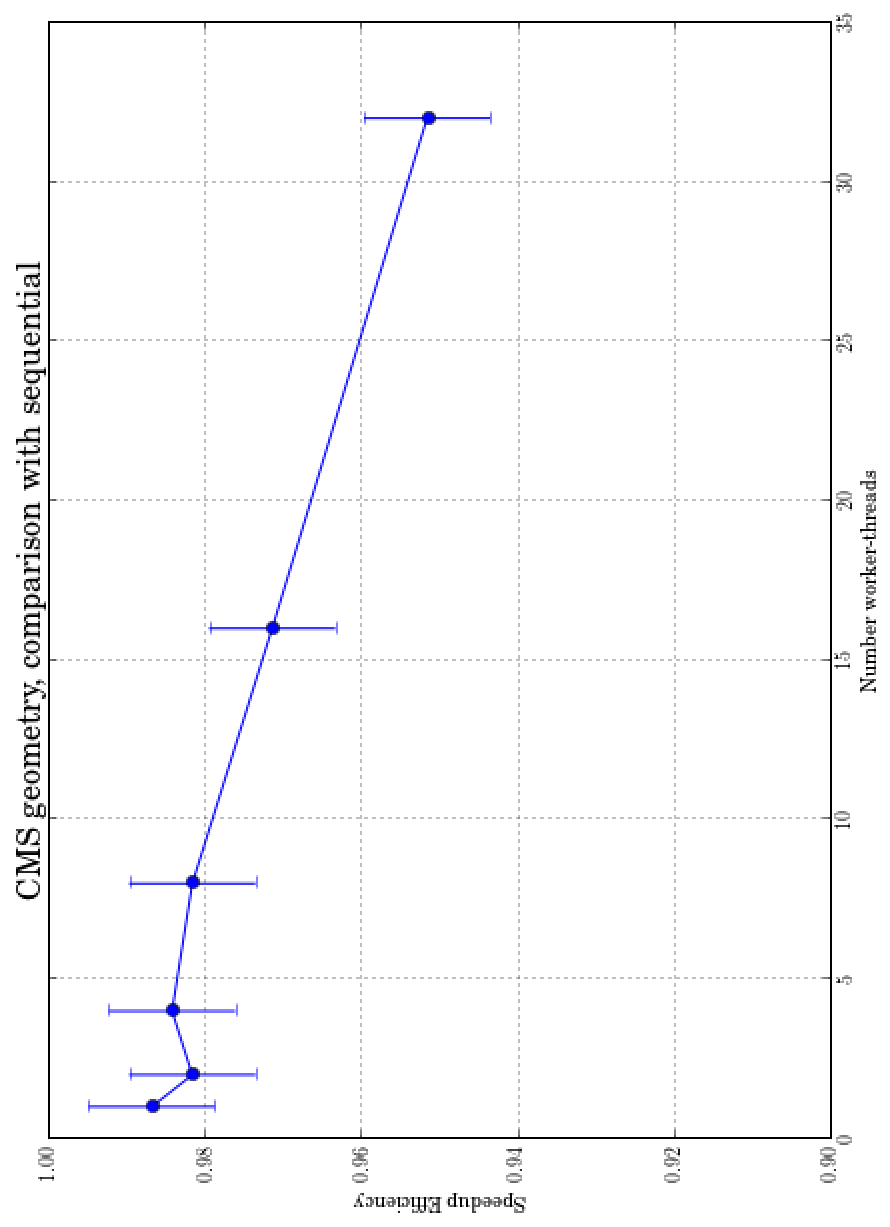
\includegraphics[width=0.35\textwidth, angle=-90]{figures/MTCPU.pdf}
  \caption{Speedup efficiency (ratio of throughput of a run with {\it k} threads
           to the throughput of the sequential version), as a function of the
           number of threads, for the CMS simulation on an AMD-equipped server
           (Opteron Processor 6128 running at 2.40Hz, 4 CPU sockets x 8 cores).
           The multithreading overhead for one thread is only 1\%, while the
           efficiency is greater than 95\% for up to the maximum number of
           threads.}
  \label{fig:MTcpu}
\end{figure}

\subsubsection{CPU and Memory performance}
The goal of event-level parallelism with threads is to reduce the memory 
footprint of parallel applications, while preserving the linear speedup of
throughput as a function of the number of physical cores.
Additional throughput is also expected in CPU architectures that support 
hyperthreading adding more workers~\cite{MT:leng2002study}.

Using the GDML geometry of the CMS application, three metrics were studied: the 
multithreading overhead with the number of threads {\it k} = 1 with respect to
a pure sequential application, the linearity of speedup as a function of the 
number of threads, and the memory reduction with respect to a multi-process 
approach.

In general, a performance penalty can be expected when comparing a sequential 
version of an application with the same version running with one worker thread.
In \Gfour{} this is due to the use of the \thread keyword that adds an additional 
indirection when accessing thread-private data. To remove this penalty a careful 
study of the use of \thread was carried out: compilation flags were chosen to 
minimize the impact of Thread Local Storage (TLS) selecting the best model for
\Gfour{} applications (\gkeyword{initial-exec}).  An overhead of ($\sim1$\%)
was measured as shown by the {\it k} = 1 point of Figure~\ref{fig:MTcpu}.

Figure~\ref{fig:MTcpu} shows the speedup linearity obtained with an AMD server
(Opteron Processor 6128 running at 2.0GHz, 4 CPU sockets x 8 cores) as a 
function of the number of threads, compared to the sequential case.  Good 
linearity was obtained with the CMS geometry simulation.  Speedup was linear 
with efficiencies of more than 95\%.  This result was confirmed on a number of 
different architectures: Intel Xeon, Intel Atom and PowerPC processors, ARM 
technology, and Intel Xeon Phi co-processors.  

Reported in Table~\ref{tab:MT:perf} is a comparison of the performance of 
different hardware executing the same CMS geometry application with the number
of threads equal to the number of logical cores.  Differences in performance 
were due mainly to the relative power of each core and the core multiplicity.  
The latest generation of Intel Xeon processor showed the best performance, 
expressed as absolute throughput (events/minute).

Figure~\ref{fig:memory} shows relative memory savings as a function of the
number of threads for the CMS geometry application.  \Gfour{} efficiently reduces
the memory used by the application when running with {\it k} threads 
({\it k}$>1$) compared to {\it k} copies of the same application.  For example, 
an application with eight threads requires about half the memory needed for 
eight clones of the sequential version of the same application.  The overhead 
with one worker thread is expected, since thread-private memory objects are
duplicated between worker and master threads.  The per-thread memory overhead
is at the level of 40--80~MB depending on the application (for the same 
application described in Table~\ref{tab:MT:perf} the sequential memory 
consumption is about 200~MB).
%  For a complex application like a HEP detector this is a good result.
 
\begin{table}[htdp]
\begin{center}
\begin{tabular}{|c|c|}
\hline
 & Throughput \\ Processor type & (events/min) \\
\hline
\hline
Intel Xeon X5650 - 2.67GHz & \\ 6 cores, x2 hyper-threaded & 320 \\
                                                 (with 12 sequential instances) & (324) \\\hline 
Intel Xeon E5-2695 v2 - 2.40GHz & \\12 cores, x2 hyper-threaded & 535 \\\hline
Intel Atom C2730 - 1.7GHz & \\ 8 cores & 74 \\ \hline
Exynos 5410 Octa Cortex-A15 & \\1.6GHz - 4 cores & 47 \\\hline
PowerPC A2 - 1.6GHz & \\ 16 cores, x4 hardware threads) & 119 \\\hline
Intel Xeon Phi 7120P - 1.238GHz & \\ 61 cores, x4 hyper-threaded & 334\\\hline
\end{tabular}
\end{center}
\caption{Comparison of different hardware when running CMS experiment geometry.
         Results show throughput (events/minute) per full processor.}
\label{tab:MT:perf}
\end{table}

% \begin{figure}[H]
\begin{figure}
    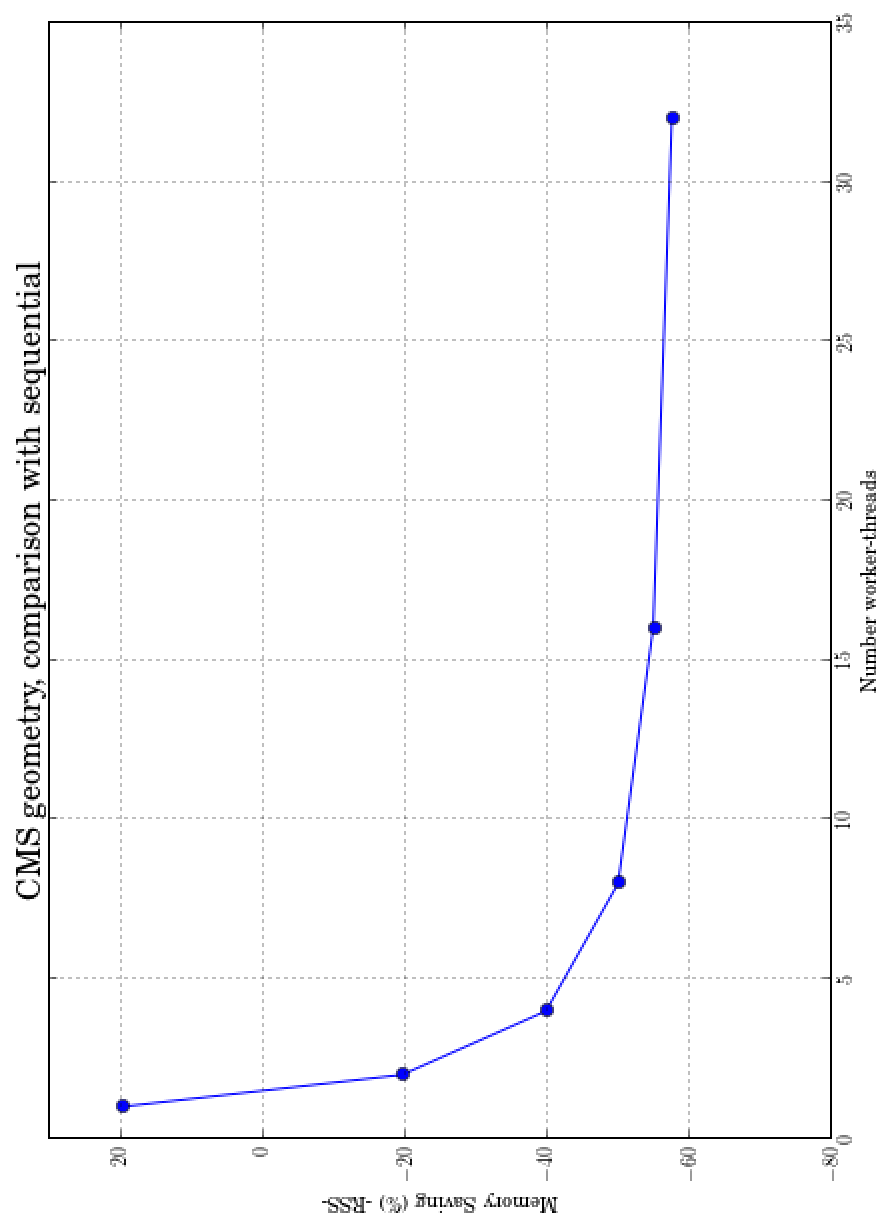
\includegraphics[width=0.35\textwidth, angle=-90]{figures/MTMEM.pdf}
  \caption{Relative memory reduction (memory used by a run with {\it k} 
           threads with respect to {\it k} instances of the sequential version),
           as a function of the number of threads, for the CMS simulation on an
           AMD equipped server (Opteron Processor 6128 running at 2.0GHz, 4 CPU
           sockets x 8 cores). The memory overhead with one worker thread is due 
           to the duplication of thread-private objects.  Already with two 
           worker threads, significant reduction of memory footprint is achieved.}
  \label{fig:memory}
\end{figure}

\subsection{\textbf{Further developments}}
Several improvements and extensions to the multithreading capabilities of 
\Gfour{} are planned for upcoming versions of the code.

With release 10.1 further reductions in the per-thread memory footprint of 
\Gfour{} applications are planned.  The most memory-consuming objects in typical 
simulations have been identified as hadronic cross sections, high precision
neutron models, reaction tables of the binary cascade models and the general 
particle source primary generator; strategies will be implemented to share these
objects among threads.  In some cases refinement of the design of the modules is
being carried out to better match the general multithreading strategy.  One goal
is to reduce the per-thread memory footprint by a factor of two.  This will 
allow applications to run on co-processors, where memory is of the order of GBs
and there are of order 100 threads.

Currently the number of threads is fixed and cannot be modified dynamically.
The planned removal of this restriction will achieve better integration with 
external parallelization frameworks such as Intel Threading Building Blocks 
(TBB)~\cite{MT:TBB}.  A prototype example,
\verb"examples/extended/parallel/TBB", that replaces \Gfour{}'s POSIX 
threading model with the TBB task-parallelism model, has already been released
with \Gfour{}, but improved and streamlined integration with this library is 
planned.

For several years now, \Gfour{} has provided an example, 
\verb"examples/extended/parallel/MPI", that demonstrates integration
with Message Passing Interface (MPI) \cite{MT:MPI}.  In version 10.0 this
example was migrated to a hybrid approach in which MPI ranks can exploit
multithreading to efficiently use memory-distributed systems.  Further 
refinement of the example is planned, with particular attention paid to 
providing merging of physics results.


\section{Kernel Functionalities}

  % Authors: Takashi Sasaki and Tsukasa Aso
  %%%%%%%%%%%%%%%%%%%%%%%%%%%%%%%%%%%%%%%%%%%%%%%%%%%
% trackscore.tex
%%%%%%%%%%%%%%%%%%%%%%%%%%%%%%%%%%%%%%%%%%%%%%%%%%%
\label{sec:trackscore}
\subsection{\textbf{Tracking and Scoring}}

\subsubsection{Design changes in tracking}

The main changes in tracking include easier physics process implementation, new
infrastructure for the re-acceleration of charged particles in electric fields, 
and ``reverse Monte Carlo''.  The problem of re-acceleration is not yet solved 
and requires further development.

Adjoint or ``reverse'' Monte Carlo has been available in \Gfour{} since release 
9.3 and modifications to tracking were required to make this possible.  The 
enabling classes have names beginning with \texttt{G4Adjoint}.  Details of these 
classes and adjoint Monte Carlo can be found in section \ref{sec:biasrev}.

\subsubsection{Concrete scorers}

In \Gfour{}, a hit is a snapshot of a physical interaction or accumulation of 
interactions of tracks in a sensitive detector component.  ``Sensitive'' here
refers to the ability of the component to collect and record some aspects of 
the interactions, and to the \Gfour{} classes which enable this collection.
Because of the wide variety of \Gfour{} applications, only the abstract classes
for both detector sensitivity and hit had thus far been provided in the toolkit.
A user was therefore required to have the expertise necessary to implement the 
details of how hits were defined, collected and stored.

To relieve many users of this burden, concrete primitive scorers of physics 
quantities such as dose and flux have been provided which cover general-use 
simulations.  Flexibly designed base classes allow users to implement their own
primitive scorers for use anywhere a sensitive detector needs to be simulated.

Primitive scorers were built upon three classes, 
\gclass{G4Multi\allowbreak{}Functional\allowbreak{}Detector},
 \gclass{G4VPrimitiveScorer} and
\gclass{G4VSDFilter}.
\gclass{G4\allowbreak{}Multi\allowbreak{}Functional\allowbreak{}Detector}
is a concrete class
derived from \gclass{G4VSensitive\allowbreak{}Detector} and attached to the
detector component.  Primitive scorers were developed on top of the base class
\gclass{G4VPrimitiveScorer}, and as such represent classes to be registered to
the \gclass{G4MultiFunctionalDetector}.  \gclass{G4VSDFilter} is an abstract
class for a track filter to be associated with a
\gclass{G4MultiFunctional\allowbreak{}Detector} or a primitive scorer.
Concrete track filter classes are also provided.  One example is a charged track
filter and a particle filter that accept for scoring only charged tracks and a
given particle species, respectively.

A primitive scorer creates a \texttt{G4THitsMap} object for storing one physics
quantity for an event.  \texttt{G4THitsMap} is a template class for mapping an 
integer key to a pointer value.  Since a physics quantity such as dose is 
generally accumulated in each cell of a detector component during an event or 
run, a primitive scorer generates a \gclass{G4THitsMap<G4double>} object that 
maps a pointer to a \gclass{G4double} for a physics quantity, and uses the cell
number as the integer key.  If a cell has no value, the \gclass{G4THitsMap} 
object has no corresponding entry and the pointer to the physics quantity 
returns a null.  This was done to reduce memory consumption, and to distinguish
an unfilled cell from one that has a value of zero.  The integer key of the cell
is taken from the copy number of the \texttt{G4LogicalVolume} of the detector 
component by default.  \Gfour{} also provides primitive scorers for 
three-dimensional structured geometry, in which copy numbers are taken at each 
of the depth levels at which of the logical volumes are nested in the geometric
structure.  These copy numbers are then serialized into integer keys. 

\subsubsection{Command-based scoring}

Command-based scoring is the easiest way to score primitive physics quantities.
It is based on the primitive scorers and navigation in an auxilliary geometry 
hierarchy (``parallel world,'' Section \ref{sec:nav}).  Users are not 
required to develop code, as interactive commands are provided to set up the 
scoring mesh.

The scoring mesh consists of a scoring volume in a three-dimensional mesh with
a multifunctional detector, primitive scorers and track filters which may be 
attached to a primitive scorer.  An arbitrary number of primitive scorers can 
be registered to the scoring mesh.

A given physics quantity, or score, is accumulated in each cell during a run. 
Interactive commands allow scores to be dumped into a file and written out in 
CSV format.  Other commands allow scores to be visualized as color histograms
drawn on the visualized geometry in either a projection or a selected profile.
 
Because scoring volumes are placed in a parallel world, the scoring volume and
the mass volume are allowed to overlap.  Command-based scoring can therefore 
obtain the physics quantity in an arbitrary volume or surface independent of the
mass volume.  One exception to this is the dose primitive scorer, in which 
the scoring volumes and their cells must coincide exactly with the mass geometry
structure.  This is because the mass density of the cell is taken from the mass 
geometry while the volume of the cell is taken from the scoring geometry. 

%
% Check that mass geometry and scoring geometry are defined elsewhere
%
Most of the command-based scoring is handled in two classes,
\gclass{G4Scoring\allowbreak{}Manager} and \gclass{G4VScoringMesh}.
\gclass{G4ScoringManger} is the administrative class of command-based scoring.
It creates a singleton object which keeps a list of registered scoring meshes,
and operates the scoring according to interactive commands and commands from 
the \Gfour{} kernel. \gclass{G4VScoring\allowbreak{}Mesh} is the base class of 
scoring meshes which represent scoring geometries.  It keeps a list of 
associated primitive scorers.  The \gclass{G4VScoring\allowbreak{}Mesh} object
creates a series of \gclass{G4THitsMap} objects in which each primitive scorer
can accumulate physics quantities in a run. 

Command-based scoring works in both sequential and multithreaded modes.  In
sequential mode, \gclass{G4RunManager} creates scoring meshes at the beginning
of a run.  After each event, the \gclass{G4THitsMap} object in
\gclass{G4VScoring\allowbreak{}Mesh} is updated by adding values in that event
to the primitive scorer.  In multithreaded mode \gclass{G4MTRunManager} creates
a master scoring manager.  Each worker thread of \texttt{G4WorkerRunManager} 
creates its own local scoring manager with scoring meshes.  However, the logical
volume of the scoring mesh is shared between master and local scoring managers.
The local scoring manager then accumulates physics quantities in the same manner
as sequential mode.  At the end of a thread, the worker run manager requests the
master run manager to merge the scores of the local scoring manager with those
of the master scoring manager. 



  % Author: Gabriele Cosmo
  % not yet complete:
  %                   John Ap.: steppers, safety, extension in field
  %%%%%%%%%%%%%%%%%%%%%%%%%%%%%%%%%%%%%%%%%%%%%%%%%%%
% detectormodeling.tex
%%%%%%%%%%%%%%%%%%%%%%%%%%%%%%%%%%%%%%%%%%%%%%%%%%%
\label{sec:detmod}

\subsection{\textbf{Detector Modeling}}

\subsubsection{Introduction}
A key component of \Gfour{} is the geometry modeler~\cite{detmodeling:modeler},
which provides a wide variety of tools and solutions for describing geometry 
setups from simple to highly complex.  Geometrical models of the LHC detectors,
for instance, easily reach millions of geometrical elements of different kinds
combined together in hierarchical structures.  The geometry modeler provides
techniques by which memory consumption can be greatly reduced, allowing regular 
or irregular patterns to be easily replicated, assembled or reflected.  This, 
combined with navigation and optimization algorithms, allow the efficient 
computation of intersections of simulated tracks with the elements composing
any geometry setup.

Recent extensions of the geometry modeler include specialized navigation
techniques and optimization algorithms to aid medical simulation studies. 
This has allowed complex geometrical models of the human body to be developed.
Extensions also include parallel navigation and tracking in layered geometries
which allow geometry setups to be superimposed on one another with minimal 
impact on CPU time.

\subsubsection{Navigation in geometries} \label{sec:nav}
The recent addition featuring ``parallel geometries'' allows the definition and
treatment of more than one independent geometry in parallel for different 
potential uses, and exploits the existing enhanced interface provided by the 
navigation system in the \Gfour{} toolkit \cite{detmodeling:parGeom}.  In 
\Gfour{} a geometry setup is in general associated with a navigator which is a
concrete instance of the \gclass{G4Navigator} class.  \gclass{G4Navigator} was 
designed such that several instances of it can be created and coexist; each 
instance can be assigned to a different geometry hierarchy.  The primary 
navigation instance is attached to the ``mass world'' which is the main geometry 
hierarchy in which the material of the setup is described;  this setup is unique
and is used for all physical interactions.

``Parallel world'' geometries may be assigned to the additional navigator objects
and may be used for example as simple ``locators'', independent of the mass 
world, to identify exact positioning in the other geometries of a particular 
point in the global coordinate system.  Each geometry must have an
independent root volume (the world volume), which contains a hierarchy of 
physical volumes.  Volumes in one world may overlap volumes in a different 
world. 

Volumes in a parallel world geometry can be associated with the read-out 
structure of a detector.  In shower parameterization studies, for example, the
simplified read-out geometry of a calorimeter could overlay its more complex
mass geometry.  Parallel worlds are also useful in importance biasing and
scoring of doses and other radiation measures.

Volumes in a parallel world may have material; these are referred to as the
``layered mass geometry''.  In this case, the material defined in a volume in
the parallel world overrides the material defined in the mass world and is 
used for the calculation of physical interactions.  If more than one parallel 
world is overlaid on the mass world, the parallel worlds are examined, in 
reverse order of their creation, to see if any volumes with materials are 
defined in them.  Any such volumes found will override the materials in all 
previously created worlds.  Because volumes in the mass geometry always have 
materials, the material to be used for physical interactions is always 
uniquely defined.

Layered mass geometry offers an alternative way of describing complicated 
shapes that would otherwise require massive boolean operations to combine 
primitive volumes.  Examples include a photo-multiplier system partially 
dipped in a noble liquid and brachytherapy seeds implanted in the CT-scanned 
voxels of a patient.  A voxel refers to a volume element which represents a 
value on a three-dimensional grid.

In addition, different parallel worlds may be assigned to different particle 
types.  Thus, in the case of a sampling calorimeter, the mass world could 
be defined as having only a crude geometry with averaged material, while a 
parallel world would contain the detailed geometry.  The real materials in the
detailed parallel world geometry would be associated only with particle types 
that require accurate tracking, such as muons, while other particle types such
as electrons, positrons and gammas would see crude, less complicated geometry 
for faster simulation.

\subsubsection{Navigation in regular geometries}
When the voxels in a geometry are numerous and of the same size and shape, a 
specialized navigator can take advantage of the regularity to deliver faster
CPU performance.  This is useful in medical physics applications in which there
could be millions of identical volumes comprising a 3-D image of a patient.
% or test phantom.  
In this case the navigator can use a regular grid to easily 
locate the incident particle in the geometry.

In the \Gfour{} implementation 
\gclass{G4Phantom\allowbreak{}Para\allowbreak{}meter\allowbreak{}isation} 
defines the regular structure of the geometry, using the parameters of dimension, 
offset and number of voxels in each of three dimensions.  \gclass{G4RegularNavigation} 
uses this parameterization to directly locate the voxel visited by tracks in the
simulation.  An option is provided which allows boundaries between contiguous
voxels to be skipped if they are of the same material, thus significantly reducing
the number of tracking steps.

Using this method of navigation, CPU speed improvement factors of three to six
have been observed.  This factor holds for pure navigation examples (no physics 
interactions) and for beams of gammas.  For the case of electrons or protons
most of the time is spent on physics instead of navigation and the speed 
improvement is substantially reduced.  Significant savings in memory consumption
(factor of seven) and initialization time (factor of two) were also seen 
\cite{detmodeling:regnav}.

\subsubsection{Exact safety}
The ``isotropic safety'' is the distance to the next volume boundary in any 
direction.  It is calculated by the navigator and is used by the multiple 
scattering process in two distinct ways.  The primary use of the safety is to
limit the lateral displacement in order to avoid crossing a boundary within a
step.  Improved safety values reduce the need for artificial restrictions in 
electron displacement, and enable it to be better simulated at particular values
of the model parameters and production thresholds.  The isotropic safety also 
sometimes influences the step size restriction from multiple scattering.  In the
default configuration of this process it has an effect only if the safety is 
larger than the primary restriction (a fraction of the range), in which case the
safety is used as the step limit.     

The estimation of the isotropic safety was improved for volumes which have 
several child volumes.  Previously only the contents of the current voxel in 
the optimization voxels structure automatically generated at initialization, 
and the boundaries of that voxel were considered.  This resulted in a distance
which could be significantly underestimated.  The new method considers enough 
voxels to obtain a precise value of the safety, while ensuring that the number 
of voxels is limited by the running estimate of the safety value.

As a result, an improved estimate of the safety is available.  This ensures 
that the value of the isotropic safety does not depend strongly on the details
of the voxelization, on the number of child volumes, or on the presence of 
volumes in a remote region of the current volume.  The extra computation cost 
was found to be negligible in a complex simulation.

\subsubsection{Improved verbosity}
The geometry modeler with its current version of the navigator offers an 
enhanced verbosity system which can be used to help developers and users in 
debugging problems or to provide closer monitoring of the execution flow and 
behavior of the navigation system during tracking.  A set of UI commands was 
defined and made available by default in the user application which allows the 
execution flow to be controlled with five different levels of detail:
\begin{verbatim}
/geometry/navigator/verbose [level-number]
 -- Setting run-time verbosity for the geometry
      navigation
    Command having effect -only- if Geant4 has
      been installed with verbose mode
      (G4VERBOSE flag) set!
    Level 0: Silent (default)
    Level 1: Display volume positioning and 
              step lengths
    Level 2: Display step/safety info on point
              locations
    Level 3: Display minimal state at -every-
              step
    Level 4: Maximum verbosity (very detailed!)
\end{verbatim}
A special UI command 
\begin{verbatim}
/geometry/navigator/check_mode [true/false]
\end{verbatim}
was also defined to modify the execution mode of the navigator and perform extra
checks for correctness, or to apply stricter and less tolerant conditions to 
stress precision.  This can help in studying and debugging difficult cases by 
eventually highlighting potential defects in the geometry under consideration.
% \begin{verbatim}
% /geometry/navigator/check_mode [true/false]
%  -- Setting navigator in -check_mode- state
%     (default is false).
%     Command having effect -only- if Geant4
%     has been installed with verbose mode
%     (G4VERBOSE flag) set!
% \end{verbatim}
An additional UI command
\begin{verbatim}
/geometry/navigator/push_notify [true/false]
\end{verbatim}
allows the enabling or disabling of notifications from the navigator for 
artificial pushes applied by the navigation system along the track direction in
case tracks get stuck in particular geometries.
% \begin{verbatim}
% /geometry/navigator/push_notify [true/false]
%  -- Setting navigator verbosity push 
%     notifications (default is true).
%     Command having effect -only- if Geant4 
%     has been installed with verbose mode
%     (G4VERBOSE flag) set!
% \end{verbatim}

These new tools, in addition to a more rationalized layout of output messages
for the information provided by the system, contribute to make the navigation
system of \Gfour{} more user-friendly and provide powerful means to users
and developers to improve the quality of their simulation programs.

\begin{figure*}
\centering 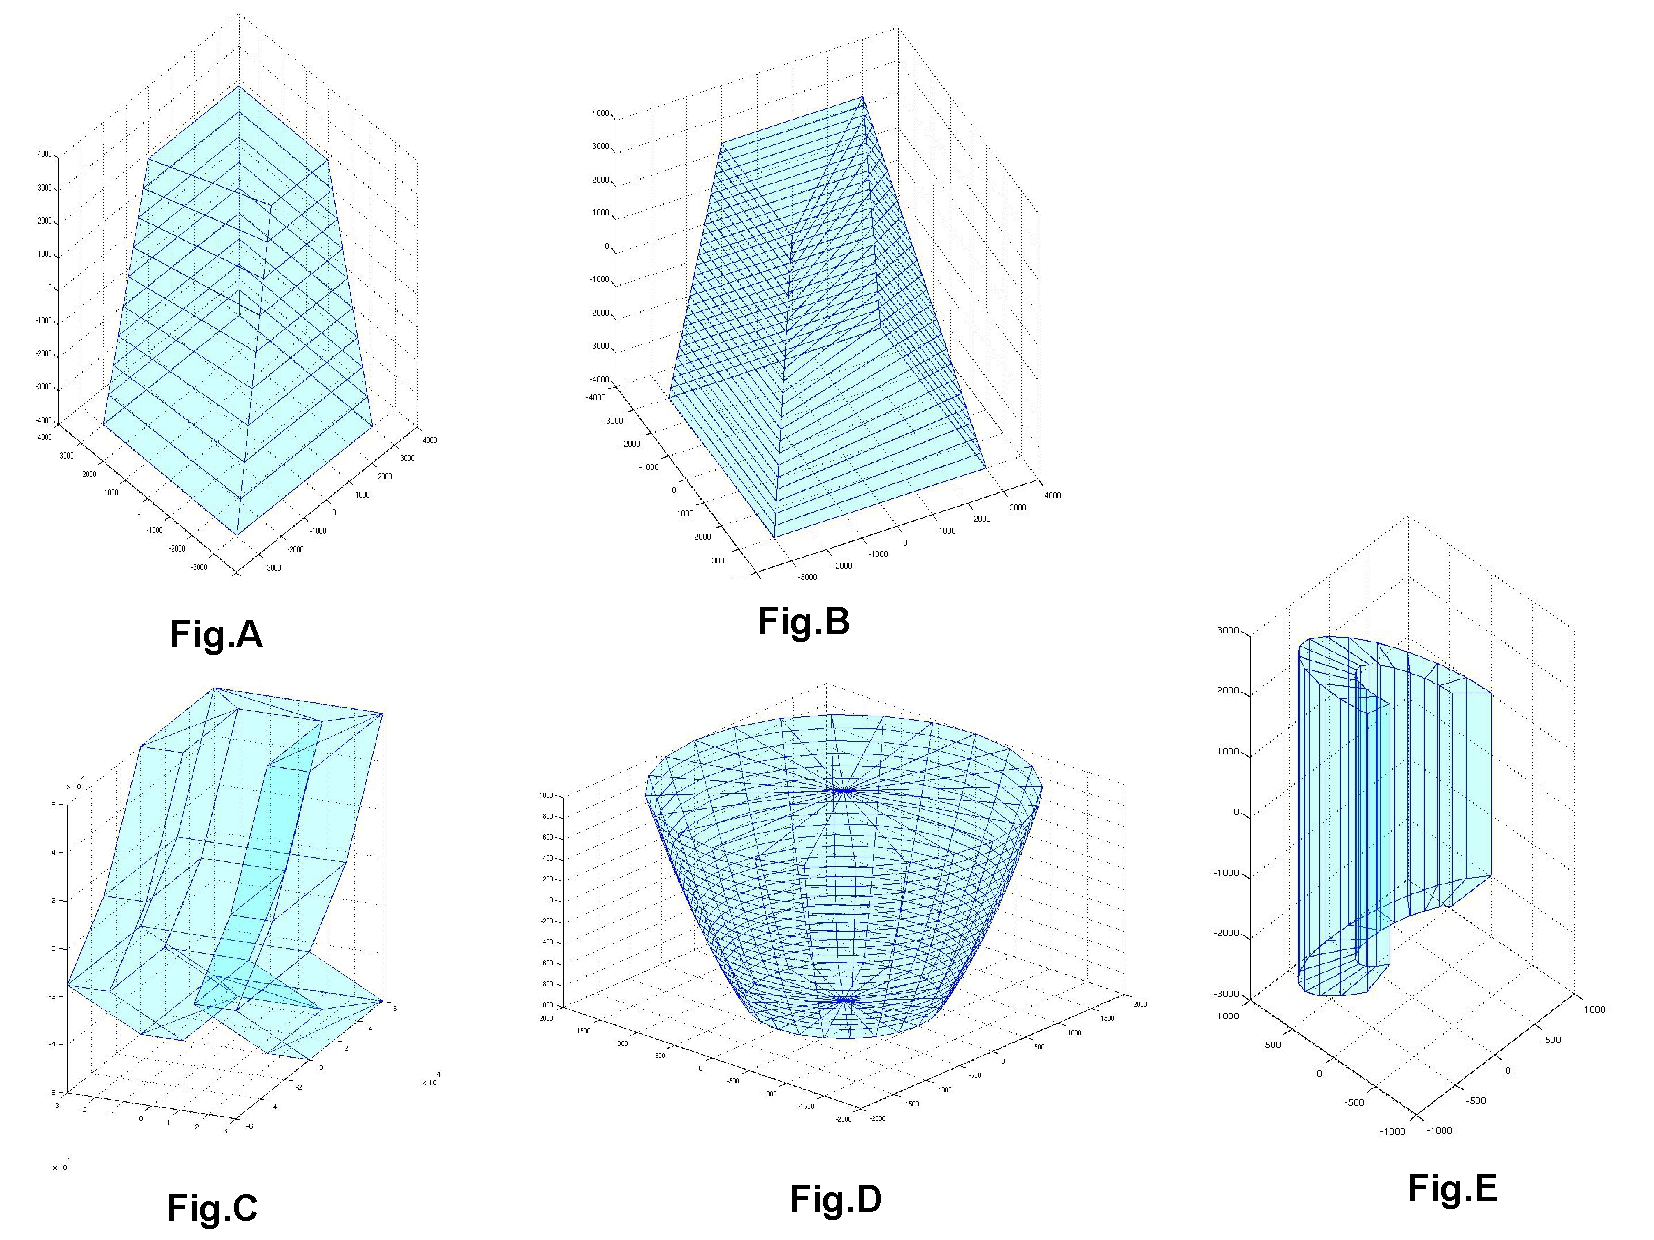
\includegraphics[height=4.0in,width=5.0in]{figures/new_solids.pdf}
\caption{Recent geometrical primitives added in \Gfour{}: generic trapezoid
         (A,B), extruded solid (C), parabolic solid (D), cut tube(E).}
\label{new_solids}
\end{figure*}

\subsubsection{Extensions to geometrical primitives}
Since \Gfour{} release series 8, new geometrical primitives, \gclass{G4GenericTrap}, 
\gclass{G4ExtrudedSolid}, \gclass{G4Paraboloid} and \gclass{G4CutTubs}, have been
part of the toolkit and are shown in Figure~\ref{new_solids}.

\gclass{G4GenericTrap} is an arbitrary trapezoid with up to four vertices lying
in each of two parallel planes at -hz and +hz perpendicular to the $z$ axis.  
Vertices are specified by their $x,y$ coordinates.  Points may be identical in 
order to create shapes with fewer than eight vertices; the only limitation is to
have at least one triangle at +hz or -hz.  The lateral surfaces are not necessarily 
planar and in that case they are represented by a surface that linearly changes
from the edge at -hz to the corresponding edge at +hz.  This represents a 
sweeping surface with a twist angle linearly dependent on $z$, which is different
from the twisted solids which have surfaces described by an equation depending on
a constant twist angle.  In Figure \ref{new_solids}A a \gclass{G4GenericTrap} 
with eight vertices and a twist is shown; Figure \ref{new_solids}B shows a
\gclass{G4GenericTrap} with collapsed vertices and a twist.

\gclass{G4ExtrudedSolid} (Figure \ref{new_solids}C) is a solid obtained by the
extrusion of an arbitrary polygon in the defined $z$ sections.  Each $z$ section
is defined by a $z$-coordinate, an offset in the $x,y$-plane and a factor by
which to scale the polygon at the given $z$ coordinate.  Each section in $z$ of
the \gclass{G4ExtrudedSolid} is a scaled version of the same polygon.  A second,
simplified constructor for the special case of a solid with only two
$z$-sections is also provided.

\gclass{G4Paraboloid} (Figure \ref{new_solids}D) is a solid with a parabolic
profile and possible cuts along the $z$ axis at +hz and -hz, with the cut planes 
perpendicular to the $z$ axis.  To construct the parabolic profile, the 
following equation is used:
\begin{verbatim}
  Z=a* (x*x+y*y)^2+b
\end{verbatim}
with real coefficients $a$ and $b$; the coefficients are calculated from given
radii at +hz and -hz.

\gclass{G4CutTubs} (Figure \ref{new_solids}E) is a tube or cylindrical section
with cuts applied in $z$.  These cuts are planes defined by a normal vector 
pointing outside the tube (cylindrical section) and intersect the $z$ axis at a
given point +hz or (and) -hz.

An important and rather useful construct for shapes delimited by any kind of 
complex surface is offered by the \gclass{G4TessellateSolid} class, which allows
complex geometrical shapes to be described by approximating their surfaces as a
set of planar facets (triangles), with tunable resolution.  This technique can
be used for importing geometries from CAD systems to generate surface-bounded 
solids.  Recent developments during the implementation of the Unified Solids
library~\cite{detmodeling:USolids}, provide considerably improved CPU 
performance, making it possible to use such constructs for very detailed and 
realistic descriptions of surfaces, while optimally scaling with the number of 
facets in use.  A sample \gclass{G4TessellateSolid} is shown in 
Figure \ref{tessellated_cpu}.
 
Unified Solids have been available since \Gfour{} 10.0 as experimental 
alternatives to the traditional geometrical primitives.  The aim is to offer
an independent library of such solids to replace the traditional primitives.

Cloning of all geometrical primitives has been possible since release 9.4, 
with the definition of appropriate copy constructors and assignment operators.
This functionality is required when running in multithreaded mode when 
parameterized geometries are used.  All solids also have the ability to compute
their own surface area and geometrical volume:
\begin{verbatim}
  G4double G4VSolid::GetSurfaceArea()
  G4double G4VSolid::GetCubicVolume() .
\end{verbatim}
A solid's surface area and geometrical volume are estimated using Monte Carlo
sampling methods when it is not possible to compute them with mathematical 
formulae;  in such cases the accuracy can be tuned in case the default does not
provide sufficient precision.  Computed values are expressed in internal units
and are cached for reuse.  In a detector setup, these utilities allow for the
calculation of the overall mass of the setup for a specific logical volume:
\vspace{2.0cm}

\begin{verbatim}
G4double
G4LogicalVolume::GetMass(G4bool forced=false,
                     G4bool propagate=true,
                     G4Material* parMaterial=0) .
\end{verbatim}
The mass of the logical volume tree expressed in internal units is computed
from the estimated geometrical volume of each solid and material associated
with the logical volume and, by default, its daughters.  The returned value
is also cached in this case and can be used for successive calls, unless
recomputation is forced by providing 'true' for the boolean argument (i.e. 
in case the geometry setup has changed after the previous call).  By setting
the ``propagate'' Boolean flag to 'false' only the mass of the current logical 
volume is returned (with the volume occupied by the daughter volumes 
subtracted).  An optional argument ``parMaterial'' can be used to specify a 
custom material for a specific logical volume; the argument is also used 
internally to consider cases of geometrical parameterization by material. 

\begin{figure}
\centering 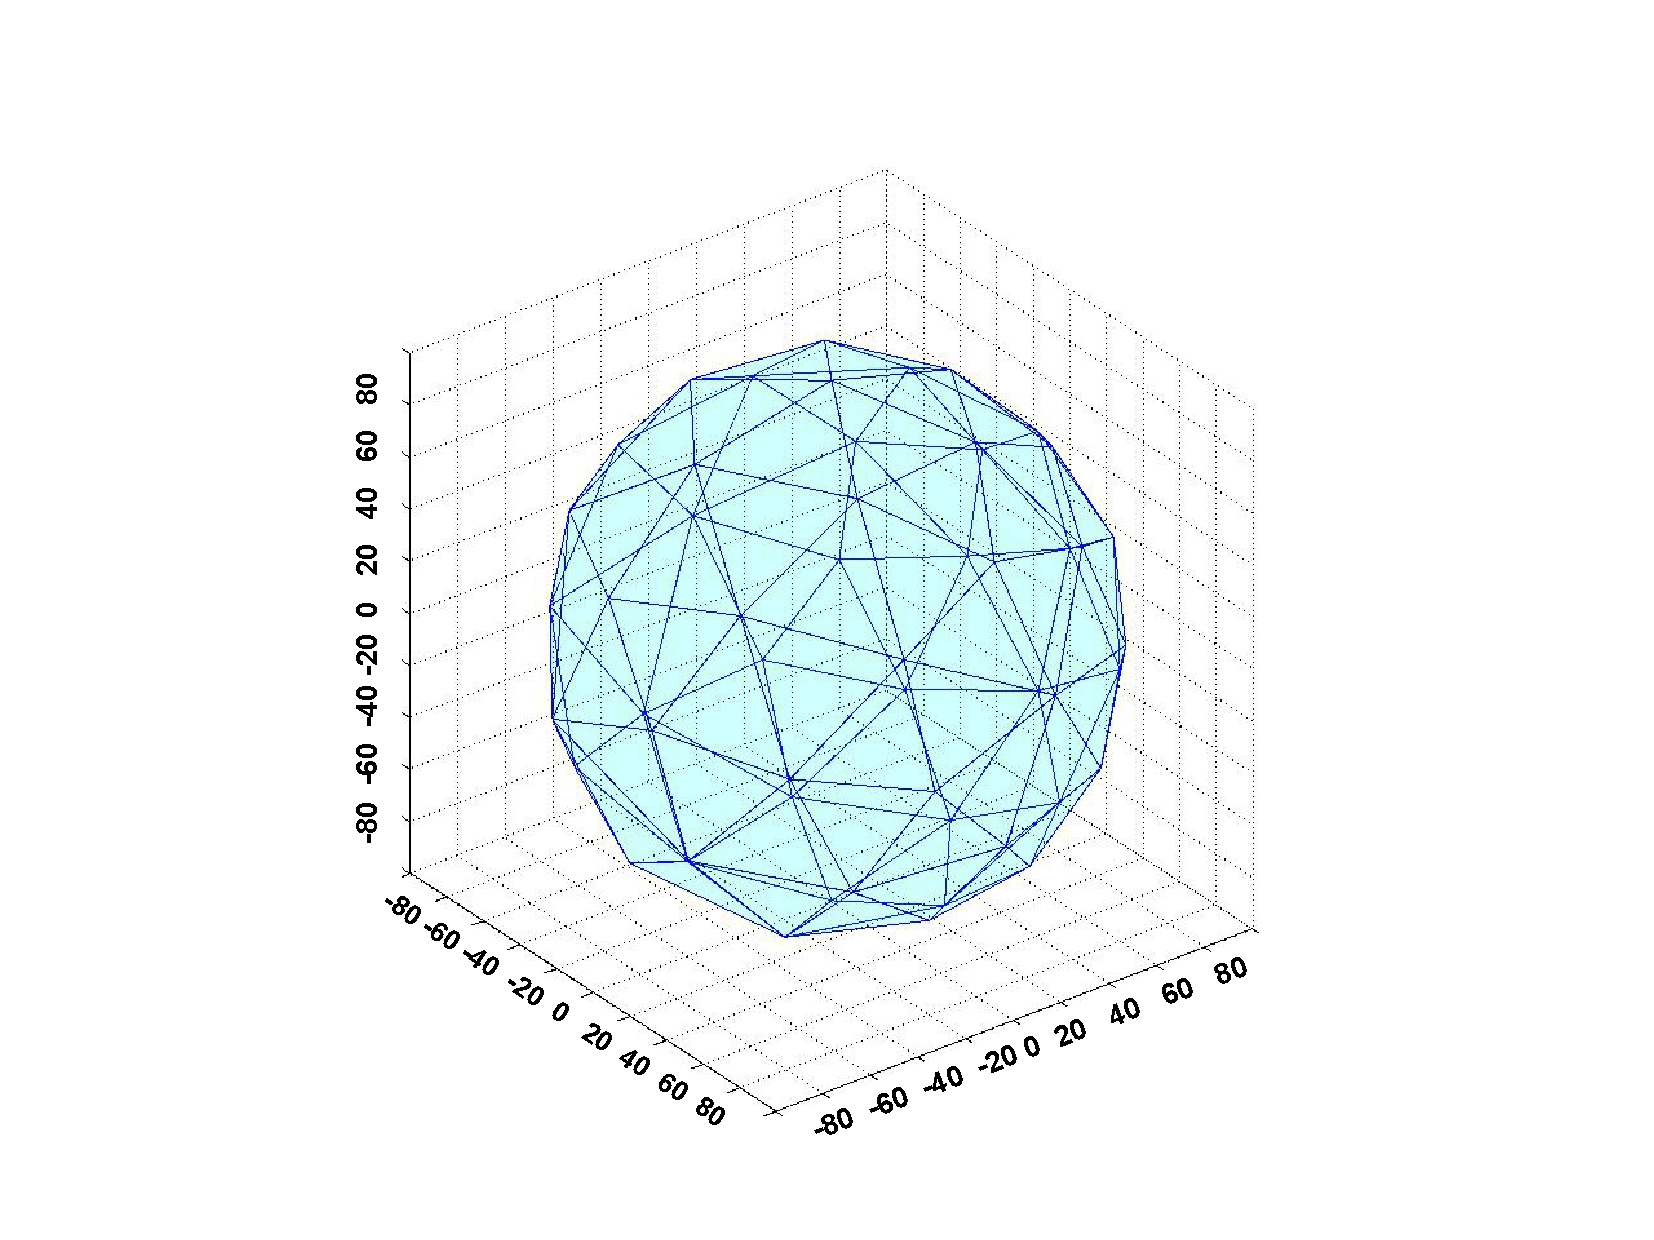
\includegraphics[height=2.5in,width=3.4in]{figures/NewSphere.pdf}
\centering 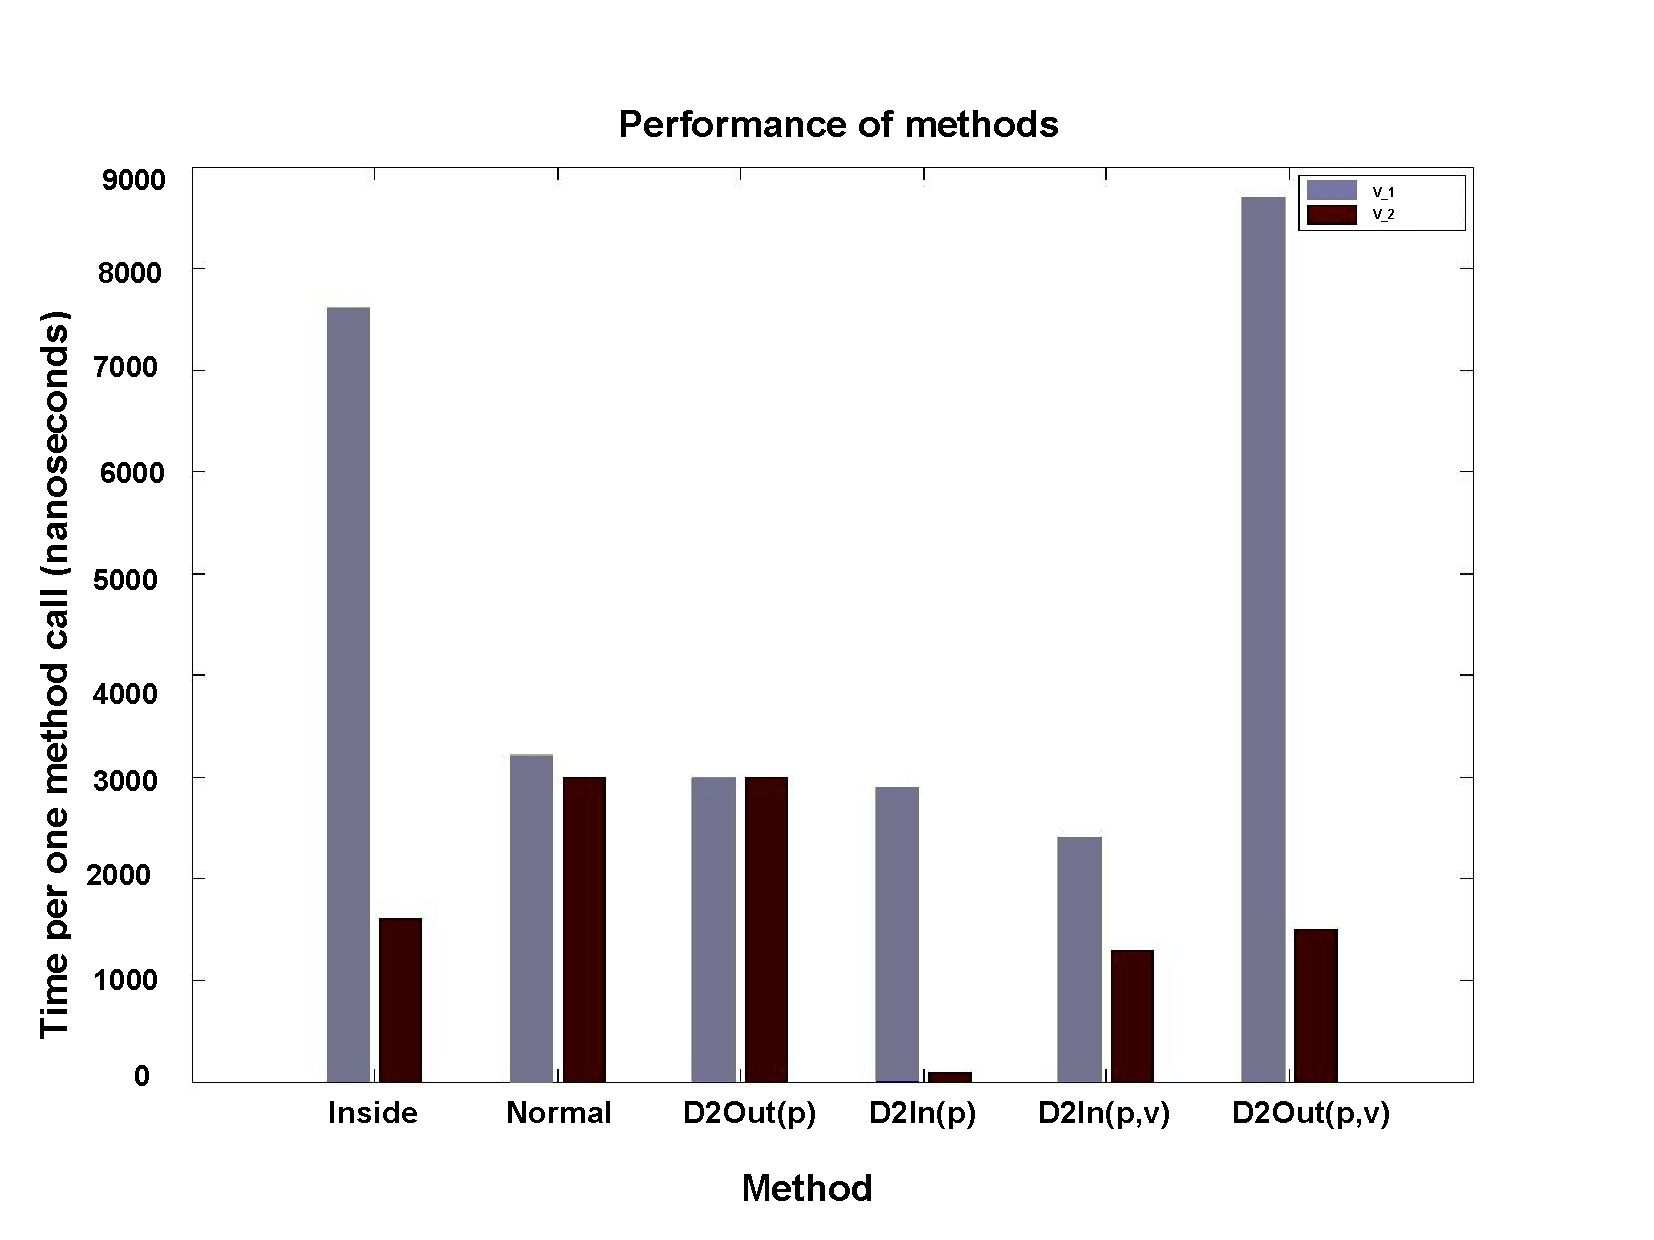
\includegraphics[height=3.4in,width=3.4in]{figures/tessellated_cpu.pdf}
\caption{Relative performance for the tessellated sphere (top), illustrated for
         each individual method.  Method name abbreviations are 
         D2In(p) : DistanceToIn(p), D2In(p,v) : DistanceToIn(p,v),
         D2Out(p) : DistanceToOut(p),  D2Out(p,v) : DistanceToOut(p,v).
         Light colored bars correspond to \Gfour{} 9.5.p02 and dark colored bars 
         correspond to \Gfour{} 9.6.p02.  Already for solids composed of a 
         relatively small number of facets (100 as in the case for the sphere), a 
         clear improvement is measured, especially for key methods.}
\label{tessellated_cpu}
\end{figure}
Since release 8.2 the geometry modeler has provided a tool to precisely identify
and flag defects in the geometry setup due to overlapping surfaces of physical 
volumes.  The technique makes use of the ability of each geometrical primitive
to randomly generate points lying on its surface and verifying that none of
these points is contained in other volumes of the same setup at the same level
in the geometry tree.  With the release 10 series, this technique is also used 
when ovelap checks are issued as UI commands, replacing the old method based on 
sampling over an overlapping grid of lines or cylinders.  These UI commands are 
listed and explained in section 4.1.11 (Detecting Overlapping Volumes) of the 
Application Developer Guide \cite{bib:AppDevGuide}.
% \begin{verbatim}
% /geometry/test/tolerance [double] [unit]
%   -- to define tolerance by which overlaps
%      should not be reported. Default is '0'.
% /geometry/test/verbosity [bool]
%   -- to set verbosity mode. Default is 'true'.
% /geometry/test/resolution [int]
%   -- to establish the number of points on
%      surface to be generated and checked for
%      each volume. Default is '10000'.
% /geometry/test/recursion_start [int]
%   -- to set the starting depth level in the
%      volumes tree from where checking 
%      overlaps. Default is level '0'.
% /geometry/test/recursion_depth [int]
%   -- to set the total depth in the volume 
%      tree for checking overlaps. Default
%      is '-1', which means checking the whole
%      tree.
% /geometry/test/maximum_errors [int]
%   -- to fix the threshold for maximum number
%      of errors to report for overlaps from a
%      volume. By default, for each volume,
%      reports stop after the first error
%      reported.
% /geometry/test/run
%   -- to start the overlaps checking
%      recursively through the volumes tree.
% \end{verbatim}

\subsubsection{Extensions to propagation in a field}
A gravitational field and the ability to create a force for it have been 
available in the toolkit since release 9.5.  Also, the force exerted on the 
magnetic moment in a gradient B-field is now taken into account for any 
particle, including neutrals.  An equation of motion was added that accounts for
the total combined force from magnetic, electric, gravitational and gradient 
B-fields as well as spin tracking.  With this it is possible to simulate the 
trajectory and spin of ultra-cold neutrons (UCN) and the trapping of neutral 
hydrogen atoms in a magnetic bottle.

A field can now be registered to a geometrical region, in addition to the global
reference frame or to a logical volume, as before.  

The mechanism to refine an intersection between a curved trajectory and volume 
boundaries was revised, making it possible to choose one of three methods or 
define a user-created method to do this.  A new multi-scale ``locator'' method 
(the new default), and a locator similar to Brent's method \cite{detmodeling:Brent} 
for root-finding, were added as alternatives to the original linear locator.
These allow the propagation in fields to cope with difficult trajectories which 
remain near to but just outside a curved surface.  This occurs in typical high 
energy physics applications which have nearly constant fields along the axis of
a tube.  The new methods also provide better overall CPU performance than the
old default, at the cost of more complex code.   

\subsubsection{Geometry persistency}
Detector geometrical descriptions can be imported and exported from text files
according to two different formats: the Geometry Description Markup Language 
(GDML)~\cite{MT:GDML} based on XML, or in plain ASCII text.  \Gfour{} provides
internal modules which allow the interpretation and conversion of the above 
formats to and from the internal geometry representation, without the need for 
C++ programming for the implementation of the various detector description 
setups.

\subsubsection*{GDML geometry}

In version 3 of GDML, the part of GDML I/O which provides the ability to
export and import detector geometry descriptions to and from GDML files, was
integrated into \Gfour{} by means of the GDML module making use of the DOM
XML parser provided with the Xerces-C++~\cite{detmodeling:XercesC} software
package.

The \Gfour{} binding for GDML implements all features supported by the \Gfour{}
geometry modeler and most of the geometrical entities defined as part of the
latest version of the GDML schema. These include all shapes, either CSG or 
specific solids, and their boolean combinations.  Also included are any 
combinations of materials, from isotopes to mixtures, and the ability to import
definitions compliant with the \Gfour{} NIST database.

All types of physical volumes are supported, from placed volumes to replicas and
parameterized volumes, including assemblies, divisions and reflections.

GDML supports the modularization of geometry descriptions to multiple GDML
files, allowing for rational organization of the modules for complex setups.
Verification of the GDML file against the latest version of the schema comes
for free thanks to Xerces-C++, with the possibility to turn it on or off in
the \Gfour{} GDML parser.

Recent additions to the GDML parser enable efficient import/export of 
tessellated solids, and the treatment of parameterizations for polycones, 
polyhedra and ellipsoids.  Release 10.1 of \Gfour{} provides support for the
definition, import and export of multi-union structures when making use of the
Unified Solids library.

Several examples are provided to illustrate most of the features of the 
\Gfour{} GDML parser:
\begin{verbatim}
examples/extended/persistency/gdml/G01
examples/extended/persistency/gdml/G02
examples/extended/persistency/gdml/G03
examples/extended/persistency/gdml/G04  .
\end{verbatim}
Example G01 shows how to write a simple application for importing and exporting
GDML files, providing a variety of samples for different kinds of solids, 
volumes, material descriptions, integration of optical surface parameters, and
so on.  Example G02 demonstrates how to import/export different geometry setups,
including STEP Tools \cite{detmodeling:STEPTools} files and structures, 
integrating them into a real simulation application.  In example G03 it is shown
how to define and import extensions to the GDML schema for attributes associated 
with a logical volume.  G04 is a simple example showing how to associate 
detector sensitivity with a logical volume, making use of the GDML feature for 
defining auxiliary information.

\subsubsection*{ASCII geometry}

The format of the ASCII text file is based on the use of tags: special words at
the beginning of each line setting what the line is describing. 

With this format the user may describe any of the geometrical objects of \Gfour{}.
It is possible to create materials combining elements, materials and detailed
isotopic composition.  Mixtures of materials can be built by providing the 
percentage of each material by weight, by volume or by giving the number of 
atoms.  The user may change the default pressure, temperature and state, or set
the minimum ionizing energy instead of letting \Gfour{} calculate it 
automatically.  Instead of explicitly building each material, predefined 
elements or materials from the \Gfour{} NIST database may be specified.
% which includes all elements from Z=1 to Z=107,
% all single-element materials from Z=1 to Z=98 and more than 200 other material
% compositions.

% \begin{figure}
%  
\includegraphics[width=0.45\textwidth]{figures/ascii_example.pdf}
% \caption{Geometry setup corresponding to the ASCII specification given in the text.}
% \label{ascii_example}
% \end{figure}

Most types of \Gfour{} solids can be described, whether CSG or specific, by
including a combination of solids through boolean operations.  Logical volumes
can be defined by attaching solids to materials, and color and visualization 
attributes can be assigned to each one.  After building the logical volumes, 
they can be placed individually or by using replicas, divisions, assemblies or
parameterizations.  As it is almost impossible with a scripting language to 
cover all the possible parameterizations a user may need, only the most common
ones are available: linear, circular, square or cubic.  If others are needed,
it is possible to define them through C++ code and mix them with the rest of
the geometry in ASCII format.  To place the volumes, rotation matrices can be
defined with three different formats providing: values of the three rotation 
angles about the three axis, the theta and phi angles that define the 
orientation of the three axes, or the elements of the 3$\times$3 rotation
matrix. 

\begin{figure}
    
\includegraphics[width=0.45\textwidth]{figures/ascii_example.pdf}
\caption{Geometry setup corresponding to the ASCII specification given in the text.}
\label{ascii_example}
\end{figure}

To facilitate the definition of a complex geometry, it is possible to use
parameters: values that can be assigned to keywords, so that they can be reused
later in any part of the geometry.  It is also possible to define numerical 
values through arithmetic expressions.
%, like
% \begin{verbatim} 
% (cos(3.)*3./sqrt(5.)) .
% \end{verbatim}
The code automatically assigns a default unit depending on the dimension: mm,
degrees, MeV, nanoseconds, $g/cm^3$, but the user may change it at any place.
Comments may be used at any point in the file, using the C++ style of placing
two forward slashes before the comment.

If the geometry description is long, it may be split into several files, which
may be combined by setting a
% \verb{#include} tag. It is also possible to
\begin{verbatim}
#include
\end{verbatim}
tag.  It is also possible to combine part of the geometry with C++ code and
another part with ASCII format.  If the user has a geometry already defined in
C++, it may be transformed into ASCII format by adding a user action in the
code.

The text format is thoroughly checked and clear error messages are provided 
when necessary.  Arithmetic expressions are checked for correctness and the 
parameters in each tag are compared against expected number and type.  An error 
message results if a line refers to a non-existent element.

An example of the geometry ASCII text format is given here and the resulting
picture is shown in Figure \ref{ascii_example}:

\begin{verbatim}
// Define a parameter for later use
:P DIMZ 5.

// Define materials
:ELEM Hydrogen H 1. 1.
:ELEM Oxygen O 8 16.
:ELEM Nitrogen N 7 14.
:MIXT Air 1.214E-03 2
      Nitrogen   0.75
      Oxygen     0.25

// Define rotation matrix
:ROTM R00  0. 0. 0.  // unit matrix

// Define volumes and place them
:VOLU world BOX 30. 30. 30. Air

:VOLU "my tube" TUBE 0. 10. $DIMZ*4 G4_WATER
:PLACE "my tube" 1 world R00 0. 0. $DIMZ

:VOLU sphere ORB 5.  G4_AIR
:PLACE sphere 1 "my tube" R00 0. 1. 10.
\end{verbatim}

% \begin{figure}
%     
\includegraphics[width=0.45\textwidth]{figures/ascii_example.pdf}
% % \centering 
\includegraphics[height=2.8in,width=3.0in]{figures/ascii_example.pdf}
% \caption{Geometry corresponding to the ASCII text file above.}
% \label{ascii_example}
% \end{figure}

An example, \verb"examples/extended/persistency/P03", is included with the 
\Gfour{} distribution to illustrate the use of the ASCII text geometry.  Several
text geometry files are provided to illustrate the many different geometry
construction options.
% possibilities:
% \begin{itemize}
% \item simple construction of materials and single placements, 
% \item isotopes, elements and materials,
% \item boolean solids,
% \item reflections,
% \item replicas,
% \item divisions,
% \item linear parameterizations,
% \item square parameterizations and
% \item assembly placements.
% \end{itemize}   	
This example also shows how to define a sensitive detector, mix C++ code with
ASCII files, extend the format to create a new tag and dump the in-memory 
geometry to an ASCII file.

% \subsubsection{Multithreading implications}
% Geometry objects are shared.
% [John, Makoto]
% Implications for user code and how to organize detector construction.
% [John, Makoto, Andrea]


  \subsection{\textbf{Visualization}}
  %%%%%%%%%%%%%%%%%%%%%%%%%%%%%%%%%%%%%%%%%%%%%%%%%%%
% visualization.tex
%%%%%%%%%%%%%%%%%%%%%%%%%%%%%%%%%%%%%%%%%%%%%%%%%%%
% \subsection{Visualization}\label{sec:viz}

\Gfour{} visualization capabilities \cite{vis:Allison} have been extended to
leverage new user interface technologies, such as Qt \cite{vis:Qt}, and to 
extend many features in response to user needs.  In many cases, visualization 
solutions that previously required extensive user coding are now provided 
through rich built-in functionality. \Gfour{} offers the user many options for
visualization drivers, some of which are always installed, others of which 
require that the user's system include particular external libraries.  
Available visualization drivers include the basic OpenGL-based \cite{vis:OGL}
drivers (OGLX, 
OGLWin32 and OGLXm), three OpenGL drivers which are more interactive (Qt, 
OpenInventor \cite{vis:OI} and OIXE) and the file-based drivers HepRApp 
\cite{vis:HPRP}, RayTracer, DAWN \cite{vis:DAWN}, VRML \cite{vis:VRML},
gMocren \cite{vis:gMoc} and ASCIITree.  Some of these drivers and new features
are detailed below.

\subsubsection{Advances in drivers and viewers}\label{sec:drv}
% Drivers.tex
The workhorses of the \Gfour{} visualization system continues to be its OpenGL
drivers.  Multiple OpenGL drivers are provided because different implementations
are required on different operating systems or for different user memory 
configurations.  For example, one flavor of OpenGL driver offers higher refresh
speed at the cost of using more memory, while another conserves memory at the
cost of speed.  The user experience has been simplified so that it is no longer 
necessary to specify which driver to use (such as /vis/open OGLI or 
/vis/open OGLSWin32).  Instead a single command (/vis/openOGL) may be issued 
from which \Gfour{} will select the most appropriate and capable viewer for the
user's current system.

Other improvements include speed increases through the streamlining of the set
of OpenGL instructions, and the ability to print any OpenGL view to high quality
output by exploiting the GL2PS \cite{vis:GL2PS} OpenGL to PostScript printing 
library.  OpenGL drivers in X11 and Qt modes allow the user to select (``pick'')
objects from the GUI in order to interrogate visualized objects, thus obtaining
track, hit or geometry information.

\Gfour{} now supports wrapping an OpenGL viewer within the versatile, highly
interactive and platform-independent Qt user interface framework.  An example of
this is shown in Figure \ref{fig:vis1}.

\begin{figure}
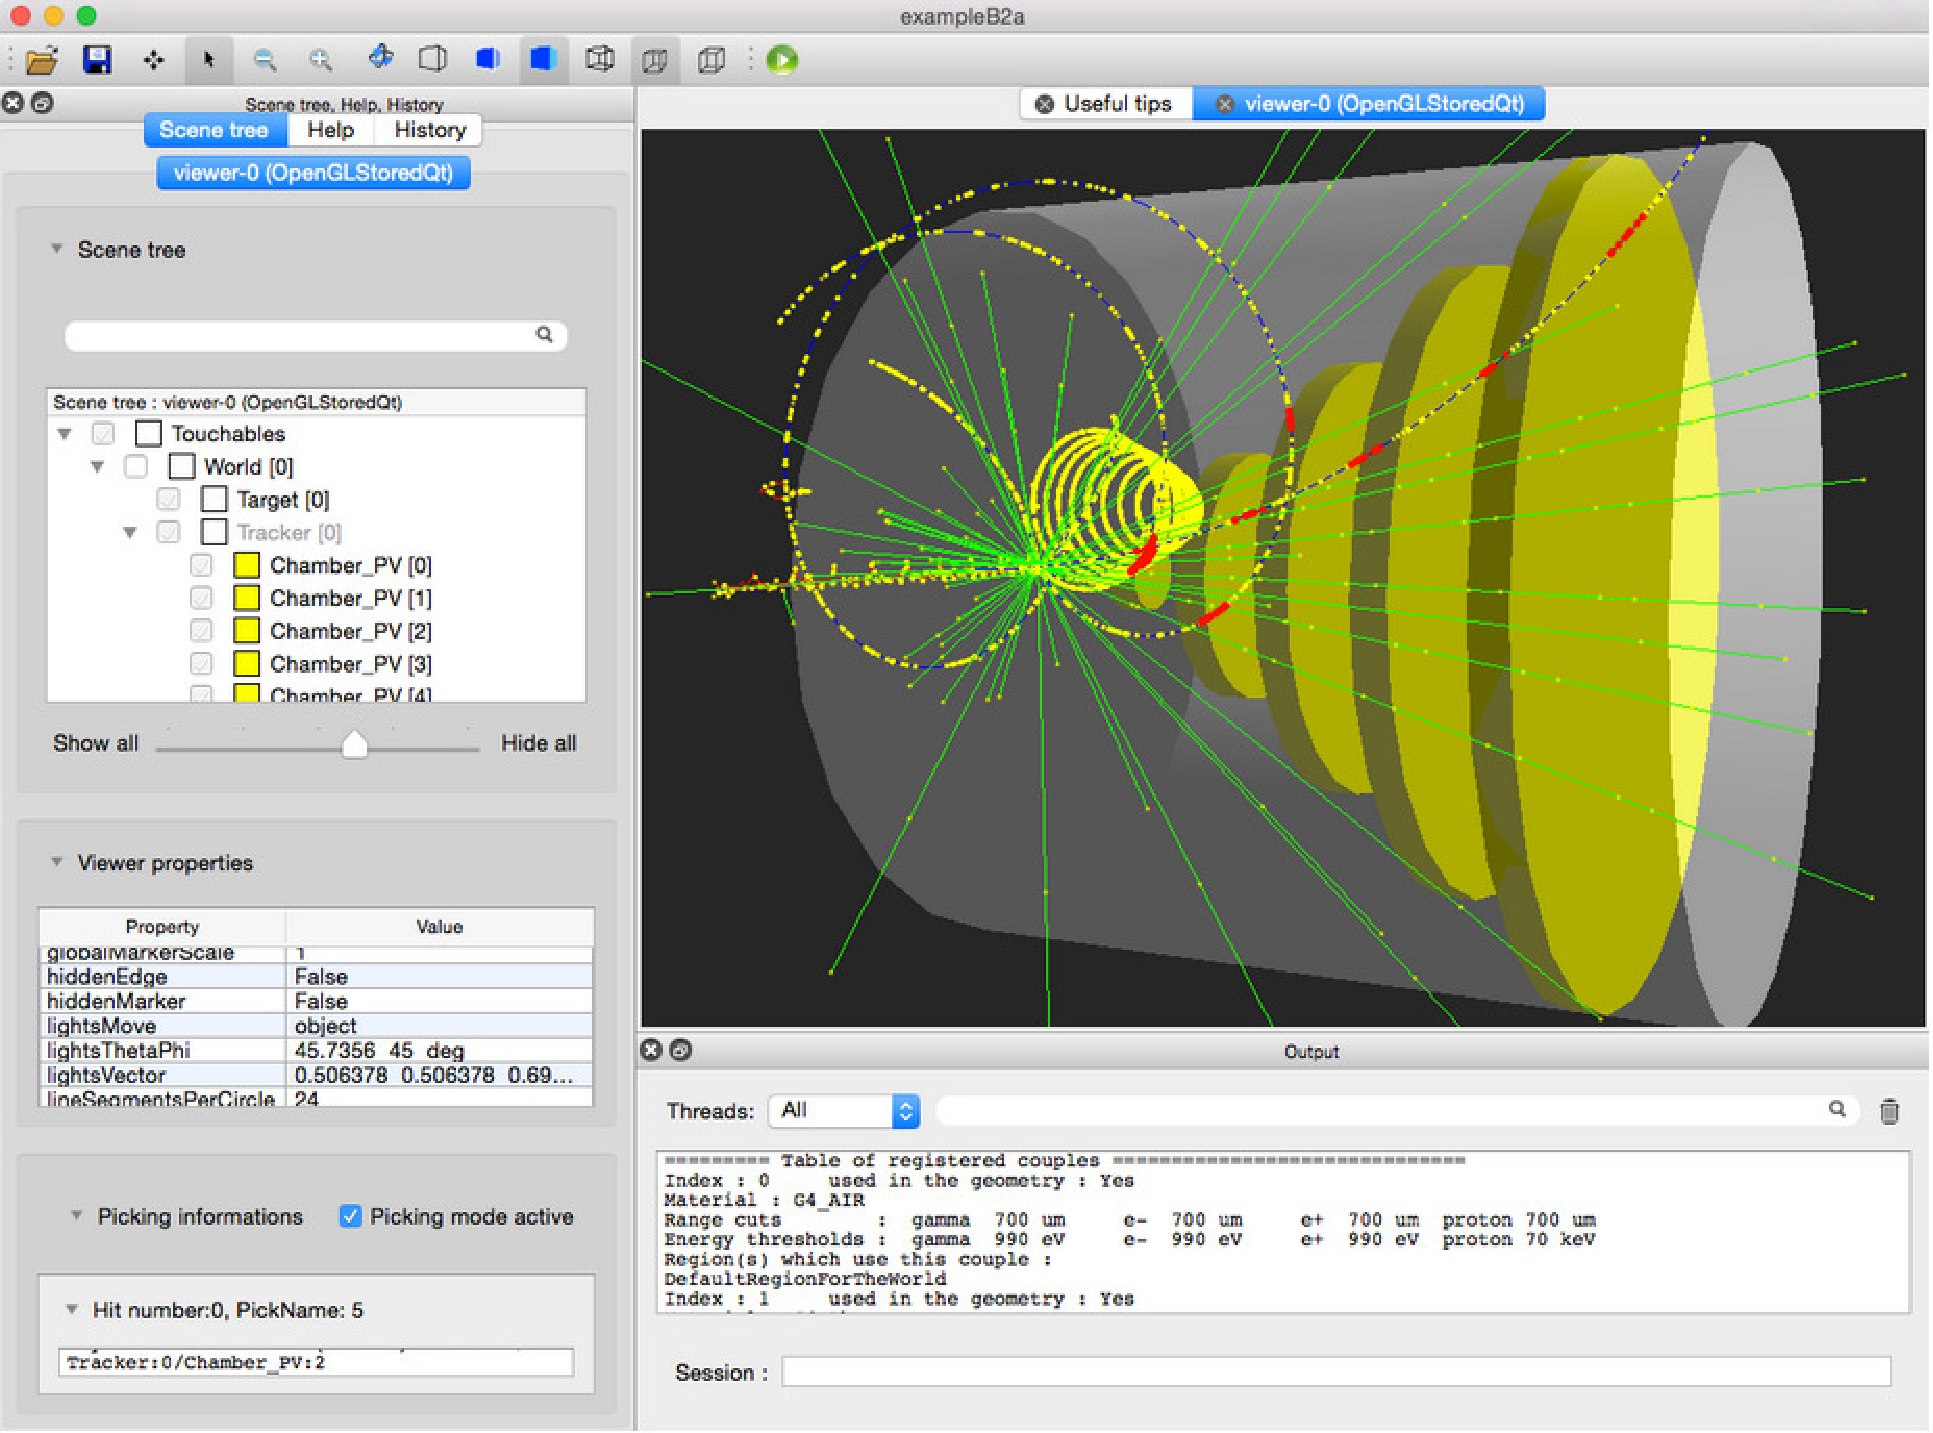
\includegraphics[width=0.47\textwidth]{figures/visfig1.pdf}
  \caption{Screenshot of OpenGL viewer wrapped in Qt.}
  \label{fig:vis1}
\end{figure}
This Qt implementation includes GUI functionality to rotate, zoom and translate
the view, and to pick visualization objects.  A slider lets the user visually
``melt away'' layers of hierarchical geometries.  Movies and EPS output are 
easily generated.  A hierarchical view of the scene's graphical elements allows 
the user to inspect and modify the color and visibility of each element.  
Another hierarchical view provides easy access to the full \Gfour{} help system.

\begin{figure}
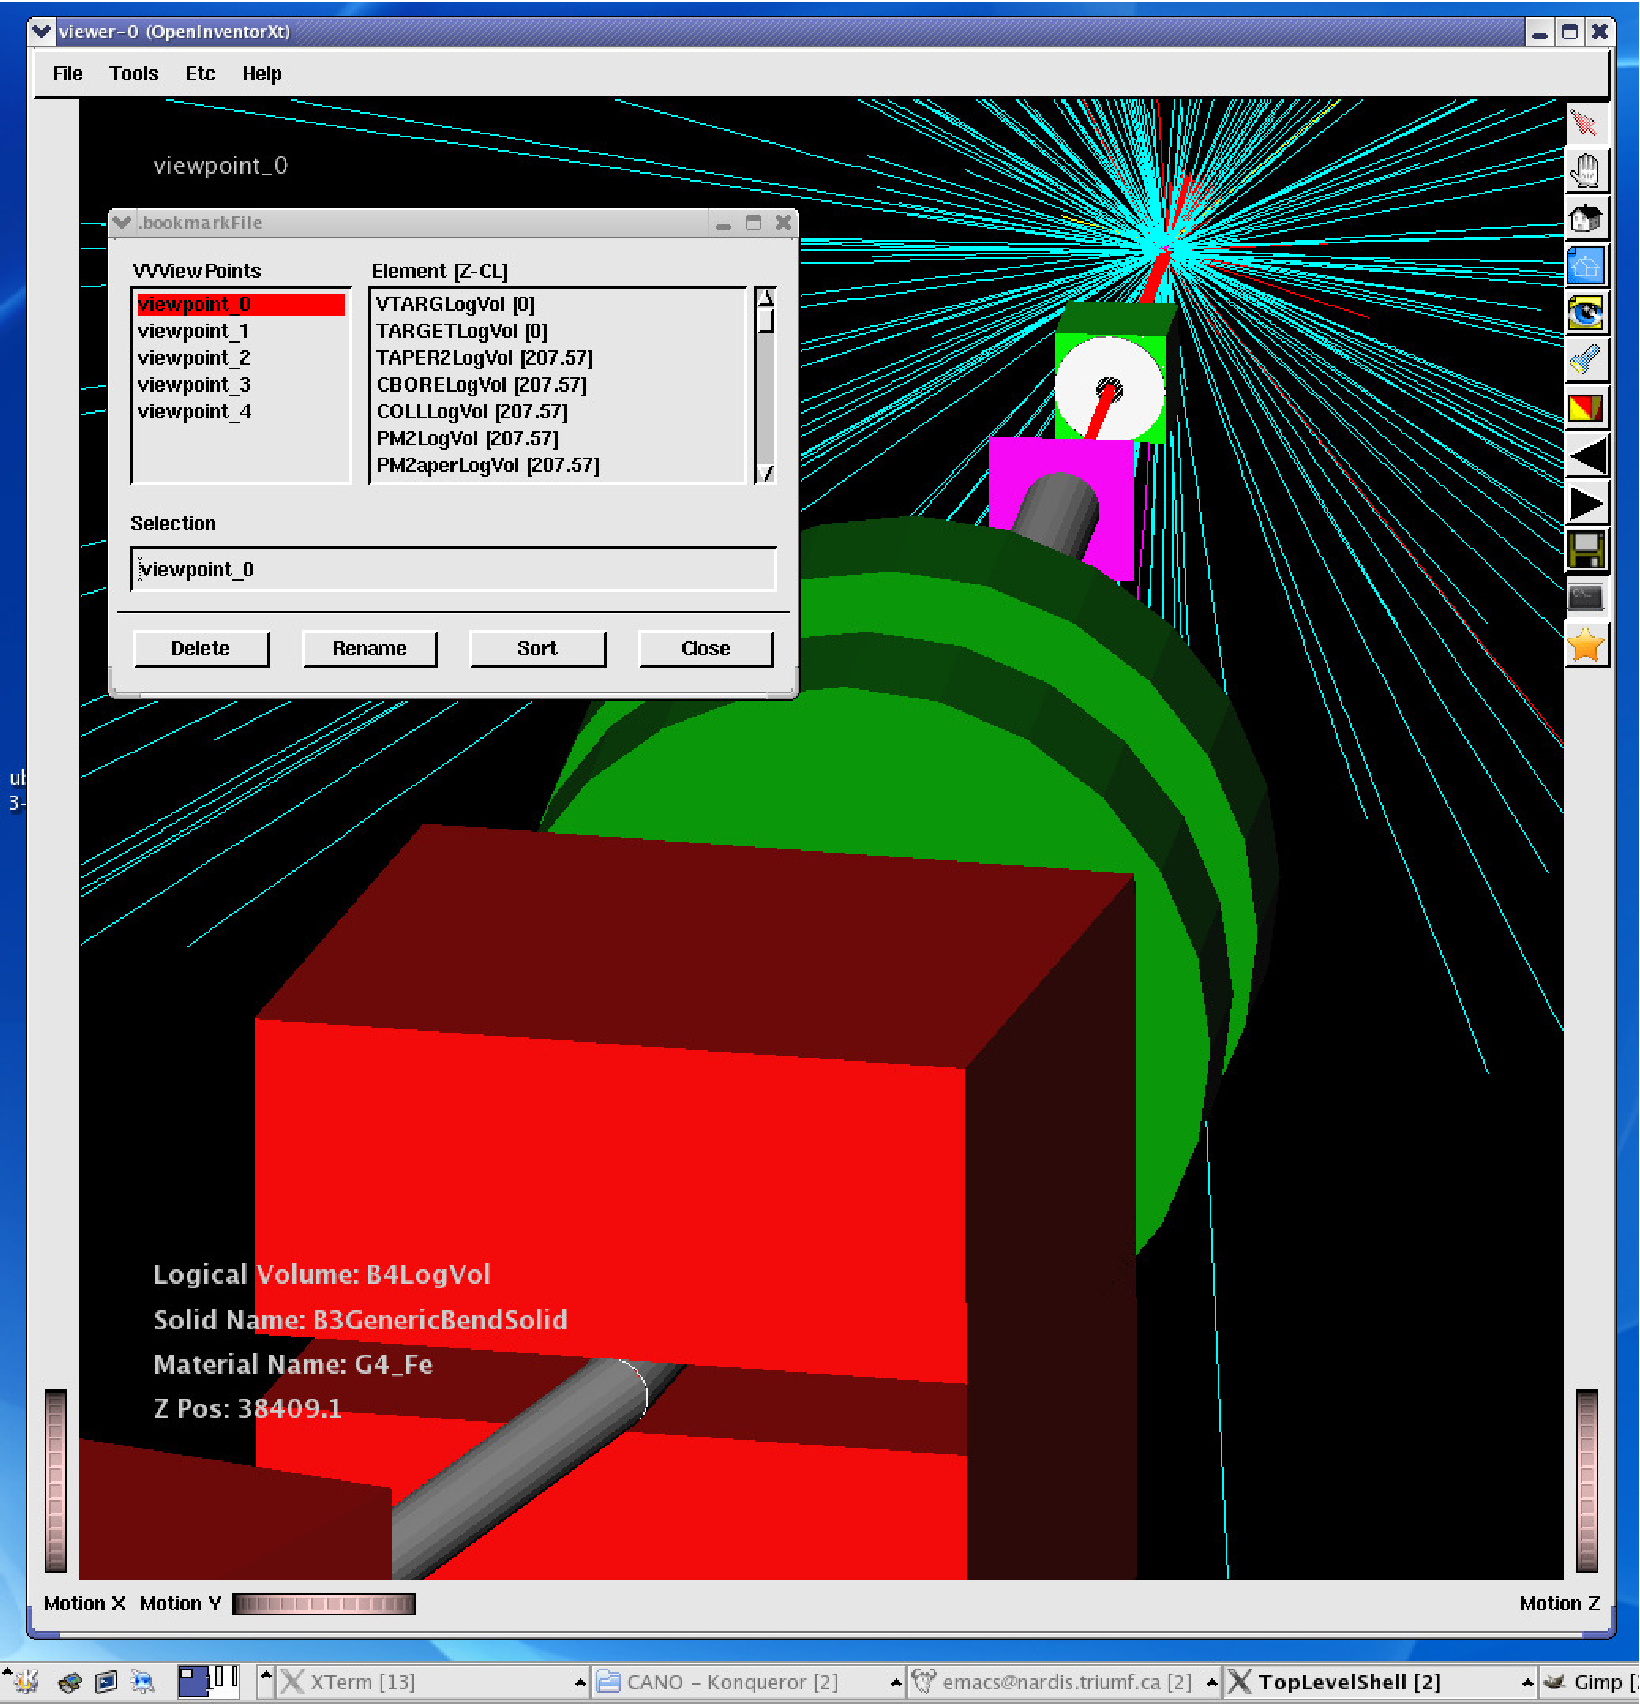
\includegraphics[width=0.47\textwidth]{figures/visfig2.pdf}
  \caption{Screenshot of Open Inventor Extended viewer.}
  \label{fig:vis2}
\end{figure}

New features have also been added to the Open Inventor (OI) driver.  The 
availability of OI greatly improved in 2011 when the Coin3D \cite{vis:coin3d} 
version of these libraries became open-source and freely available.  \Gfour{} 
made extensive use of the Coin3D classes that extend the original SGI OI 
library, creating a distinct new ``extended'' driver OIXE while leaving the 
basic driver OIX unchanged.  Figure \ref{fig:vis2} shows an example of the OIXE
viewer. 

A feature implemented in this area was the ability to save the current view and
return to it at any later time in the current or future runs.  Views are saved 
and accumulated in a bookmarks file specified by the user.  Each view is tagged
with a user-provided or default name, and all views are listed in a scrolling 
auxiliary window.  Clicking on a view name restores the view, or a sequence of 
views can be walked through via the keyboard's arrow keys.  All viewpoint and 
camera parameters are stored in ASCII form allowing editing or external 
generation of bookmarks.

As in other OpenGL viewers, object selection from the GUI is supported on 
trajectories, hits and geometry.  The OI driver provides both normal trajectory 
picking, where all trajectory points are shown, and reduced picking, where only
the first and last points are shown.  The viewer also supports mouse-over 
picking, whereby the element data is displayed directly in the viewer window 
when the mouse pointer is hovered over any object.

The remaining new developments concern moving the camera along a reference
path.  They are motivated by accelerator and beam line geometries, but may be
useful for other large and/or extended structures.  The reference path, defined
in a piecewise linear fashion by an ordered set of points, may be read from a 
file or copied from any particle trajectory.  Once a reference path is 
established, a navigation panel lists all elements in the geometry, ordered by
their distance along the reference path (based on the shortest distance 
\cite{vis:polyline} from the element center to the path).  The panel may then
be used to extract information on the elements or rotate the camera around them.
% moves the camera immediately to a centered view of that 
% element, and the arrow keys can then be used to rotate the camera around the 
% element in precise 90-degree steps around the local axes.  The shifted left and
% right arrow keys provide smooth movement of the camera along the reference path.
% OI capabilities have been used to render these motions smoothly so as not to be
% jarring to the eye.  During camera movement, a continuous readout of the 
% distance along the reference path is given.

A Reference Path Animation mode moves the camera continuously along the path, 
allowing a fly-through giving a particle's-eye view of the geometry.  Keyboard 
controls adjust animation speed and direction and allow adjusting the camera 
angle to obtain fly-overs and fly-unders.



\subsubsection{New feautures in trajectory modeling and filtering}\label{sec:trajectory}

Many options are now provided for how trajectories should be modeled (how colors
or line styles are selected).  These improvements have eliminated the most 
common reason users had to code their own trajectory classes.  In addition to 
the default model, where trajectories were colored by charge, one can now set 
color or other line properties based on particle ID, particle origin volume, or
any other particle attribute that has been loaded into a \texttt{G4AttValue}.
One can also add entirely new, customized trajectory models.  New options make
it easy to control whether trajectories are shown as basic lines, lines plus
step points or step points alone, and one may also modify step point colors.

Additional new features allow trajectories to be filtered, causing only a 
specific subset to be drawn.  These filtering options match the design of the 
trajectory modeling options, so that filtering based on charge, particle ID, 
particle origin volume, or some custom aspect, is possible.  Filters may be
daisy-chained so that one may show, for example, only the neutrons originating
from a particular collimator.

Completing the set of additions to trajectory drawing is the ability to select
smooth and rich trajectories.  By default, trajectories are represented as a set
of line segments connecting particle steps.  Because \Gfour{}'s efficient 
stepping algorithm may require very few steps in some magnetic fields, the 
default trajectory drawn through a solenoidal field may appear very jagged.  The
optional Smooth Trajectory Drawing causes additional points to be generated
along the particle trajectory so that the visualization is smoother.  Rich 
trajectories concern the amount of additional information with which 
trajectories and step points are annotated.  By default, trajectories have only 
basic information attached and step points have only position information; thus 
when one picks on these objects in the various pick-enabled viewing systems 
(HepRApp, Qt, OI or OpenGL with X11), one discovers only a few pieces of 
information about the trajectory and no details about the trajectory points.  
The Rich trajectory option enriches this annotation, providing picked 
trajectories containing many more pieces of information, such as the entire 
history of geometry volumes traversed.  It also adds a wealth of information to
step points, such as the type of process that created the step.



\subsubsection{Additional new features}\label{sec:morefeatures}

% NewFeatures.tex
Time Slicing was added to allow one to produce movies that show the time
development of an event.  With time slicing enabled, the OpenGL line segments
that represent a particle trajectory are annotated with time information.  Users
can then select an OpenGL view that corresponds to a given time, and a sequence
of such views produces the frames of a time development movie.  Users can 
produce these movies in any OpenGL viewer by the appropriate use of \Gfour{}
command macros.  The Qt driver provides a simplified way for users to make such
movies.

\Gfour{} visualization now has the ability to retain the pointers to 
previously-viewed events, so that after visualizing a set of events, one can go
back to the beginning of the set and review the events.  When coupled with 
customized user code that specifies which events should be kept, one can 
potentially run a very large set of events and then afterwards choose to 
visualize only those events that satisfied some personal set of trigger 
conditions.

The following features have also been added:
\begin{itemize}
\item parallel worlds, including layered mass worlds, may now be viewed
      individually or superimposed on the main geometry world;

\item magnetic fields may be displayed as a set of arrows indicating local
      field direction, with arrow lengths proportional to field strength;

\item decorations are now supported which allow the user to easily annotate
      graphical views with text (placed either in 3D coordinates or 
      in the 2D coordinates of the graphics window), run and event number,
      arrows, axes, rulers, date stamps and logos;

\item users may adjust the visibility or appearance of geometry by using the 
      /vis/geometry commands which globally modify the appearance of some set of
      geometry objects, while the /vis/touchable commands allow control of these
      objects individually.
\end{itemize}



\subsubsection{Approach to MT}\label{sec:approachMT}

The final set of changes concern \Gfour{}'s migration to multithreaded (MT) 
operation.  The overall design of visualization remains little-changed for 
those users running in sequential mode, but significant changes were required 
to enable visualization from MT mode.

Currently in MT mode, events are only drawn at end of run, that is, once all
threads have completed their work.  This limitation is scheduled to be removed
in release 10.2 by moving part of visualization to its own thread, such that 
each event is available for drawing as soon as that event is complete.

In MT mode, visualization will properly handle any commands that request drawing
of high level graphical objects (geometry volumes, trajectories and decorations
such as axes).  However, user-supplied code that directly asks the visualization 
system to draw low level graphical primitives (polygons or polylines) is not 
supported.  This limitation will not likely affect many \Gfour{} users, as 
recent improvements to geometry, trajectory and decoration handling have made 
such user-supplied code largely unnecessary.  Because significant work will be 
required to remove this limitation, support will come only if there is strong 
demand for these features in MT mode.

The RayTracer driver has itself been been multithreaded to take maximum 
advantage of MT.





\section{Recent Developments in Physics Modeling}
  %%%%%%%%%%%%%%%%%%%%%%%%%%%%%%%%%%%%%%%%%%%%%%%%%%%
% emphyiscs.tex
%%%%%%%%%%%%%%%%%%%%%%%%%%%%%%%%%%%%%%%%%%%%%%%%%%%
\subsection{\textbf{Electromagnetic physics}}\label{sec:emphys}
The \Gfour{} set of electromagnetic (EM) physics processes and models 
\cite{bib:G4,bib:uni,embib:design} are used in practically all types of
simulation applications including high energy and nuclear physics experiments,
beam transport, medical physics, cosmic ray interactions and radiation effects
in space.  In addition to models for low and high energy EM physics for 
simulation of radiation effects in media, a sub-library of very low energy 
models was developed within the framework of the \Gfour{}-DNA project, with the
goal of simulating radiation effects involving physics and chemistry at the 
sub-cellular level \cite{embib:dna3}.

\subsubsection{Unification of EM physics sub-packages}\label{sec:em1} % JMCB Feedback
% Author: Omrane Kadri
%%%%%%%%%%%%%%%%%%%%%%%%%%%%%%%%%%%%%%%%%%%%%%%%%%%
% uni.tex
%%%%%%%%%%%%%%%%%%%%%%%%%%%%%%%%%%%%%%%%%%%%%%%%%%%
In the early stages of \Gfour{}, low and high energy electromagnetic processes
were developed independently, with the result that these processes could not
be used in the same run.  To resolve this problem, the interfaces were unified
so that the standard, muon, high energy, low energy and DNA EM physics 
sub-packages \cite{bib:uni} now follow the same design.

All \Gfour{} physical processes, including transportation, decay, EM, hadronic,
optical and others, were implemented via the unique general interface
\gclass{G4VProcess}.  Three EM process interfaces inherit from it via the 
intermediate classes \gclass{G4VContinuousDiscreteProcess} or 
\gclass{G4VDiscreteProcess} \cite{embib:design}:
\begin{itemize}
\item \gclass{G4VEnergyLossProcess}, which is active along the step and post
              step,
\item \gclass{G4VMultipleScattering}, which is active along the step and
\item \gclass{G4VEmProcess}, which has no energy loss and is active post step
              and at rest. 
\end{itemize}
These three base classes are responsible for interfacing to the \Gfour{} kernel, 
initializing the electromagnetic physics, managing the energy loss, range and 
cross sections tables, managing the electromagnetic models, and the built-in 
biasing options.  Each process inherits from one of these base classes, and has
one or more physics models.  EM physics models were implemented via the 
\gclass{G4VEmModel} interface.  A model is applied for a defined energy range 
and \gclass{G4Region}, allowing, for example, one model from the low energy and 
one from the high energy sub-package to be assigned to a process for a given 
particle type.

Migration to this common design resulted in an improvement of overall CPU 
performance, and made it possible to provide several helper classes which are 
useful for a variety of user applications:
\begin{itemize}
\item \gclass{G4EmCalculator}: accesses or computes cross section, energy loss,
              and range;
\item \gclass{G4EmConfigurator}: adds extra physics models per particle type, 
              energy, and geometry region; 
\item \gclass{G4EmSaturation}: adds Birks saturation of visible energy in
              sensitive detectors;
\item \gclass{G4ElectronIonPair}: samples ionization clusters in tracking
              devices.
\end{itemize}

These common interfaces enabled the full migration of EM classes to
multithreading \cite{embib:chep14} with only minor modifications of the existing
physics model codes.  Initialization of the energy loss, stopping power and 
cross section tables is carried out only once in the master thread at the
beginning of simulation and these tables are shared between threads at run time. 

Further improvements were made through the factorization of secondary energy and
angle sampling.  The \gclass{G4VEmAngularDistribution} common interface allows
the reuse of angular generator code by models in all EM sub-packages.  The
implementation of a unified interface for atomic deexcitation, 
\gclass{G4VAtomDeexcitation} provides the possibility of sampling atomic 
deexcitation by models from all EM sub-packages.
 
The consolidation of the EM sub-packages boosts the development of new models,
% and automatically resolves a number of problems seen in previous versions.
% Moreover, it 
provides new opportunities for the simulation of complex high energy and low 
energy effects and enables better validation of EM physics \cite{embib:uni2}. 

\label{sec:emuni}

\subsubsection{Gamma models}\label{sec:em2} %JMCB Feedback
% Author: Jeremy Brown
%%%%%%%%%%%%%%%%%%%%%%%%%%%%%%%%%%%%%%%%%%%%%%%%%%%
% gamma.tex 
% Coordinator J. M. C. Brown
%%%%%%%%%%%%%%%%%%%%%%%%%%%%%%%%%%%%%%%%%%%%%%%%%%%
% \begin{figure}
% 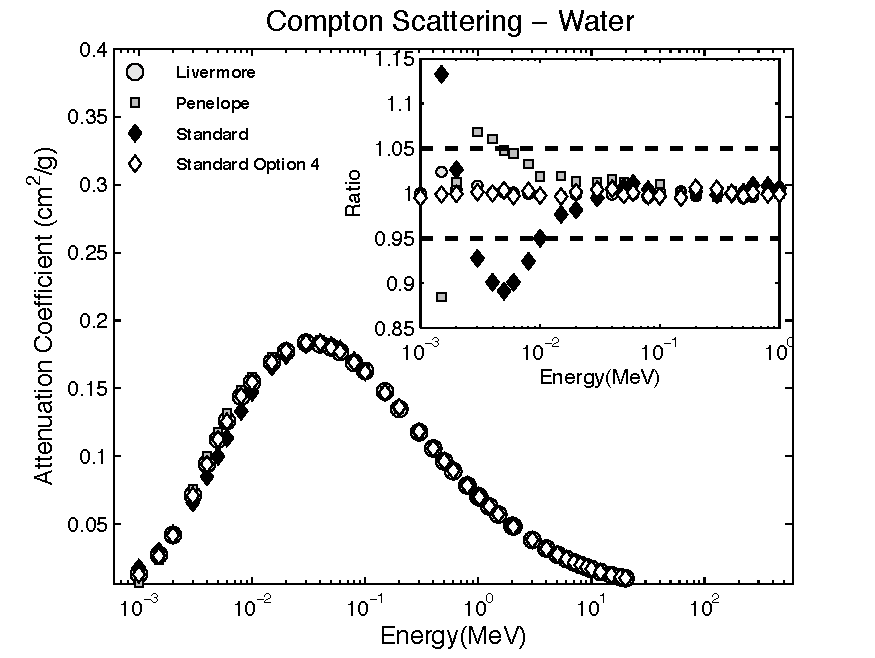
\includegraphics[width=0.5\textwidth]{figures/plot_compton.pdf}
% \caption{Compton scattering attenuation coefficient, calculated for different
%          \Gfour{} models. \gclass{G4LowEPComptonModel} is used in the Option4
%          EM physics configuration.  The inset shows the ratio of the coefficient
%          calculated using each alternative \Gfour{} electromagnetic physics list,
%          to the value from NIST XCOM \cite{embib:gamma16}.  The 
%          dashed lines correspond to a $\pm 5$\% difference.}
% \label{em:compton}
% \end{figure}
The basic set of gamma models in the EM physics packages includes models
developed for HEP applications \cite{bib:G4}, models based on the Livermore
evaluated data library \cite{embib:epdl} and a C++ implementation of the 
Penelope 2008 model \cite{embib:pen}.  Recent releases of \Gfour{} have included
revised versions of existing models, and the addition of new gamma physics 
processes and models. The low and high energy models were improved and display
similar accuracy in their shared domain of validity \cite{embib:uni2}. 
These modifications not only increased model accuracy but increased 
computational efficiency and enabled sharing of internal physics tables, 
where possible, in MT mode \cite{embib:chep14}.  
New gamma models were added to take into account physics effects not available
previously in \Gfour{} or in other simulation codes. 

A new relativistic pair production model, 
\gclass{G4Pair\allowbreak{}Production\allowbreak{}RelModel}, was developed for
simulations in astrophysics, 
LHC experiments, and other HEP applications.  This model takes into account 
the Landau-Pomeranchuk-Migdal (LPM) effect \cite{embib:gamma5}, which describes
the decrease of pair production cross sections at ultra-relativistic energies 
for dense media \cite{embib:gamma6}.  This model is physically accurate only
above 100 MeV, as no lower energy corrections are included.  It is suggested for
use in HEP applications above 80 GeV.  The use of the relativistic model is 
essential for the accurate simulation of new physics at LHC.

Two new gamma conversion models were developed to take into account the effect
of gamma ray polarization:
\begin{itemize}
\item \gclass{G4LivermorePolarized\allowbreak{}GammaConversionModel} and
\item \gclass{G4BoldyshevTripletModel} (to be used in unison with
      \gclass{G4Livermore\allowbreak{}NuclearGamma\allowbreak{}ConversionModel}).
\end{itemize}
The first is responsible for sampling electron-positron pair production by 
linearly polarized gamma rays with energies above 50 MeV \cite{embib:gamma11},
while the second (currently valid only above 100 MeV) simulates the pair 
production process in the electron field with the emission of an 
additional recoil electron \cite{embib:gamma12}, properly taking into account 
the so-called ``triplet'' production total cross section.

The Livermore polarized gamma conversion model is based on the Heitler cross
section, where the azimuthal distribution of the pair was obtained by 
integrating the cross section over energy and polar angles \cite{embib:gamma11}.

The Boldyshev triplet model uses Borselino diagrams to calculate the cross 
sections \cite{embib:pol3}.  Most of the recoil electrons in the Boldyshev model
have low energy, with a peak around $8/(T/mc^2)$, expressed in MeV, where $T$
is the gamma energy and $m$ is the electron rest mass.  Thus, a model for the
cross section was developed including a momentum threshold value of 1 $mc$, in
order to avoid the generation of too many very low energy recoil electrons
\cite{embib:pol4}. 

Finally, a specialized Compton scattering model 
\gclass{G4Low\allowbreak{}EPCompton\allowbreak{}Model} was 
developed \cite{embib:gamma13,embib:gamma14}.  Through the implementation of a
theoretical foundation that ensured the conservation of energy and momentum in
the relativistic impulse approximation \cite{embib:gamma15}, this model
implements energy and directional algorithms for both the scattered photon and 
ejected Compton electron developed from first principles. It was developed to 
address the limited accuracy of the Compton electron ejection algorithms present
in other low energy Compton scattering models that have been observed below
5~MeV \cite{embib:gamma14,embib:gamma7,embib:gamma8}. Figure \ref{em:compton} 
shows the comparison of different \Gfour{} Compton scattering cross sections
versus NIST evaluated data \cite{embib:gamma16} calculated with the methodology 
described in \cite{embib:gamma17}.  The \gclass{G4LowEPComptonModel} agrees with
the reference data to within
1\%, the statistical uncertainty of the simulation results.  The Penelope and 
Standard models result in differences up to 10\% with respect to the NIST data
for energies between 2 and 10~keV.  At higher energies, the differences are 
smaller and are below 1\% above 100 keV, corresponding to the statistical 
uncertainty of the simulation results.
\begin{figure}
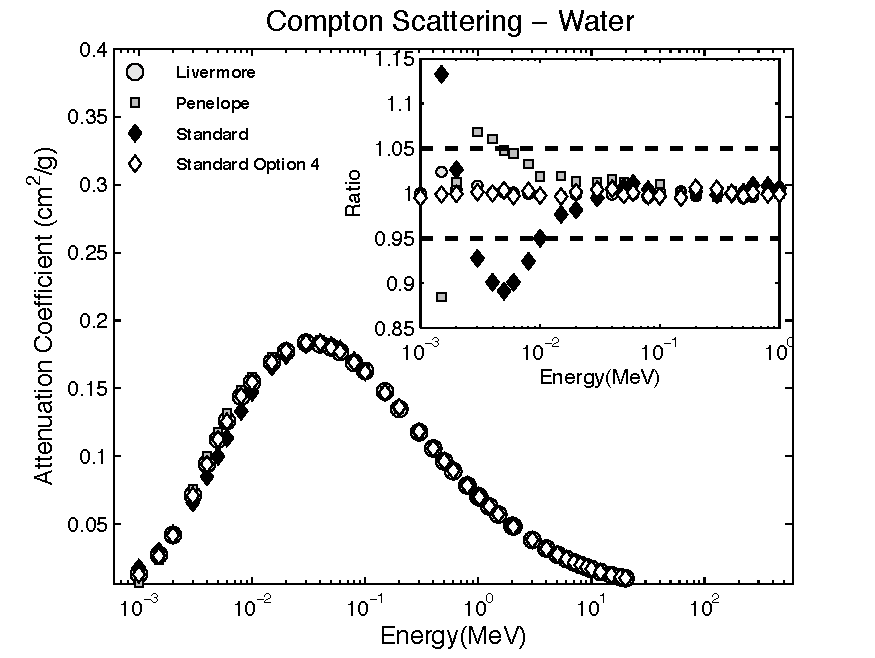
\includegraphics[width=0.5\textwidth]{figures/plot_compton.pdf}
\caption{Compton scattering attenuation coefficient, calculated for different
         \Gfour{} models. \gclass{G4LowEPComptonModel} is used in the Option4
         EM physics configuration.  The inset shows the ratio of the coefficient
         calculated using each alternative \Gfour{} electromagnetic physics list,
         to the value from NIST XCOM \cite{embib:gamma16}.  The
         dashed lines correspond to a $\pm 5$\% difference.}
\label{em:compton}
\end{figure}



\subsubsection{Ionization models}\label{sec:em3} % JMCB Feedback
% Author: Melanie Raine
%%%%%%%%%%%%%%%%%%%%%%%%%%%%%%%%%%%%%%%%%%%%%%%%%%%
% ioni.tex
%%%%%%%%%%%%%%%%%%%%%%%%%%%%%%%%%%%%%%%%%%%%%%%%%%%

\Gfour{} offers a range of ionization models for different particle types.  These 
models can be classified as either condensed or discrete.  In the condensed 
approach, the energy loss calculation has a continuous component and a discrete
one, discriminated by a given energy threshold.  Below this threshold the energy
loss is continuous, and above it the energy loss is simulated by the explicit 
production of secondary electrons \cite{embib:design}.  The user does not 
directly define the threshold because in \Gfour{} a special method of threshold 
calculations for different materials is used.  The user defines a unique 
\emph{cut in range}  \cite{bib:G4}, whose value is transformed into a kinetic 
energy threshold per material at initialization time of \Gfour{}.  Electrons 
with this kinetic energy have a mean range in a given material equal to the cut
in range and gammas have an absorption length 1/5 of the range cut.

If no value is given in the reference physics lists the default cut value of 
0.7 mm is used, providing sufficiently accurate simulation results for many 
applications.  For a specific use-case, \emph{cut in range} values should be 
optimized per geometry region.  It is recommended that this value be defined to
be less than the smallest size of geometry volumes in the region.
 
The \emph{cut in range} approach may be used for other processes besides 
ionization.  These cuts may be defined for gammas, electrons, positrons, and 
protons, and modified based on particle type and geometry region.  However, the
cut value cannot be arbitrary.  Because \Gfour{} ionization models usually have an
energy range of applicability, there is a lower limit to the electron production 
threshold.  By default the lower limit is 1 keV, but it can be changed by the 
user.  On top of this, any EM model may establish its own lower limit for the 
threshold.  If several models are applied for a given particle type, then the 
maximum of all limit values from the models is used for the particle.  For most 
ionization models the low limit is equal to the mean ionization potential of a
material. 

The list of main ionization processes and models following the condensed 
simulation approach is shown 
in Table \ref{Table-Ioni}. 
\begin{table*}
\caption{List of \Gfour{} ionization processes and models with recommended energy range.}
\label{Table-Ioni}
\begin{center}
\begin{tabular}{llll}
\hline
Particle& Process& Model& Energy range\\ \hline
 e-/e+& \gclass{G4eIonisation} & \gclass{G4MollerBhabhaModel} & 10 keV - 10 TeV\\
 e-/e+ & & \gclass{G4PenelopeIonisationModel} & 0.1 keV - 5 GeV\\
e- &  & \gclass{G4LivermoreIonisationModel} & 0.1 keV - 1 MeV \\
all & & \gclass{G4PAIModel} &   0.1 keV -  10 TeV  \\
all & & \gclass{G4PAIPhotModel} & 0.1 keV -  10 TeV \\
muons & \gclass{G4MuIonisation} & \gclass{G4BraggModel} & 0.1 keV -  0.2 MeV \\
& & \gclass{G4BetheBlochModel} & 0.2 MeV -  1 GeV \\
& & \gclass{G4MuBetheBlochModel} \cite{embib:emmu}& 1 GeV -  10 PeV \\ 
hadrons& \gclass{G4hIonisation} & \gclass{G4BraggModel} & 1 keV -  2 MeV\\
& & \gclass{G4BetheBlochModel} & 2 MeV -  10 TeV \\
& & \gclass{G4ICRU73QOModel} \cite{embib:empbar} &  5 keV -  10 MeV \\
ions & \gclass{G4ionIonisation} & \gclass{G4BraggIonModel} & (1 keV - 2 MeV)/u \\
& & \gclass{G4BetheBlochModel} & (2 MeV -  10 TeV)/u \\
 & & \gclass{G4IonParametrisedLossModel} \cite{embib:emIon}&  (1 keV - 1 GeV)/u \\
\hline
\end{tabular}
\end{center}
\end{table*}

In the condensed approach, a model of energy loss fluctuations must be used in
conjunction with the energy loss model.  The \gclass{G4VEmFluctuationModel} 
interface was developed to accommodate several implementations of fluctuation
sampling, and several models derive from it:
\begin{itemize}
\item \gclass{G4UniversalFluctuation} - default model applicable to all charged 
particles based on a previous model \cite{embib:fluc};
\item \gclass{G4IonFluctuations} -  for small steps uses
\gclass{G4UniversalFluctuation} and for big steps uses a gaussian width based
on a parameterization \cite{embib:ionfluc};
\item \gclass{G4PAIModel} and \gclass{G4PAIPhotModel} - photo-absorption 
ionization (PAI) models \cite{embib:pai}.
\end{itemize}
PAI models simultaneously provide cross sections and energy loss, and sample
energy loss fluctuations.  The ionization cross sections of the PAI models
derive from gamma absorption cross sections per atomic shell.  They are, in 
general, more accurate and stable versus simulation conditions (cuts, step 
limits, energy) than the default model \cite{embib:chep14,embib:chep11}, but are
more computationally expensive because of the internal sampling at each
ionization collision.  An illustration of simulation performance is shown in 
Figure~\ref{em:alice} for the test beam data of the ALICE Time Projection 
Chamber \cite{embib:tpc1,embib:tpc2}. 

Other studies show that PAI models generally fit the data 
independently of the step size, while the default model strongly requires the
application of extra step limitations. 

In the case of thin absorbers, the default model requires at least two particle
steps within the defined volume.  While having some difficulties for thin 
layers, the default model provides good physics performance for a variety of 
applications, in particular for tracking devices (Figure~\ref{em:silicon}), 
satisfying the requirements of most HEP experiments.

\begin{figure}
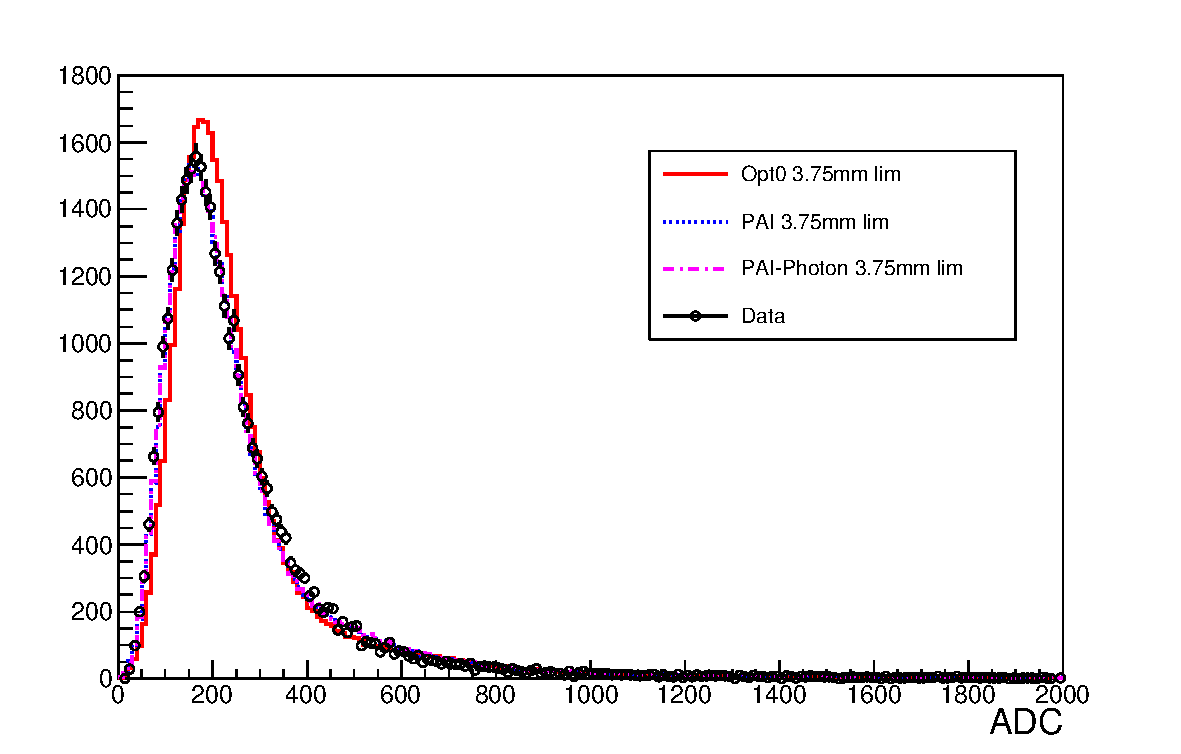
\includegraphics[width=0.5\textwidth]{figures/A_p_3gev_1mm.pdf}
\caption{Proton energy deposition in gas gap in ADC counts for a beam momentum 
         of 3 GeV/c and a gas mixture of $Ne-CO_2-N_2$.  
         The histogram represents the simulation with a 1 mm cut and a step limit
         equal to half the gap thickness.  The ADC scale for simulation was 
         normalized to the PAI model peak position.  The open circles display
         the data \cite{embib:tpc1,embib:tpc2}.}
\label{em:alice}
\end{figure}

\begin{figure}
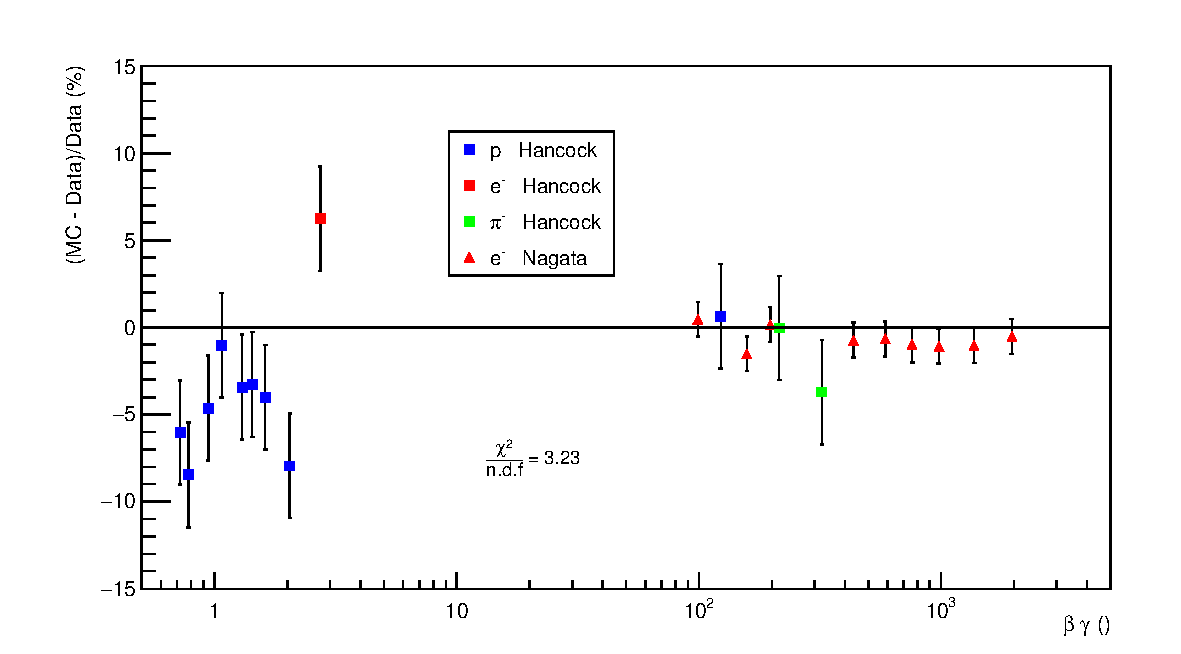
\includegraphics[width=0.5\textwidth]{figures/BetaGamma_Delta_diff_opt0_10um.pdf}
\caption{\Gfour{} versus data comparison of the most probable energy deposition in 
         thin layers of silicon (thickness 300 $\mu m$ Hancock; 1565 $\mu m$ Nagata). 
         Different beam particles and energies are used from the review
         \cite{embib:bicsel}.  Results are given in percent, and the default EM 
         physics is applied with a cut in range of 100 $\mu m$.}
\label{em:silicon}
\end{figure}

\begin{figure}
% \centering
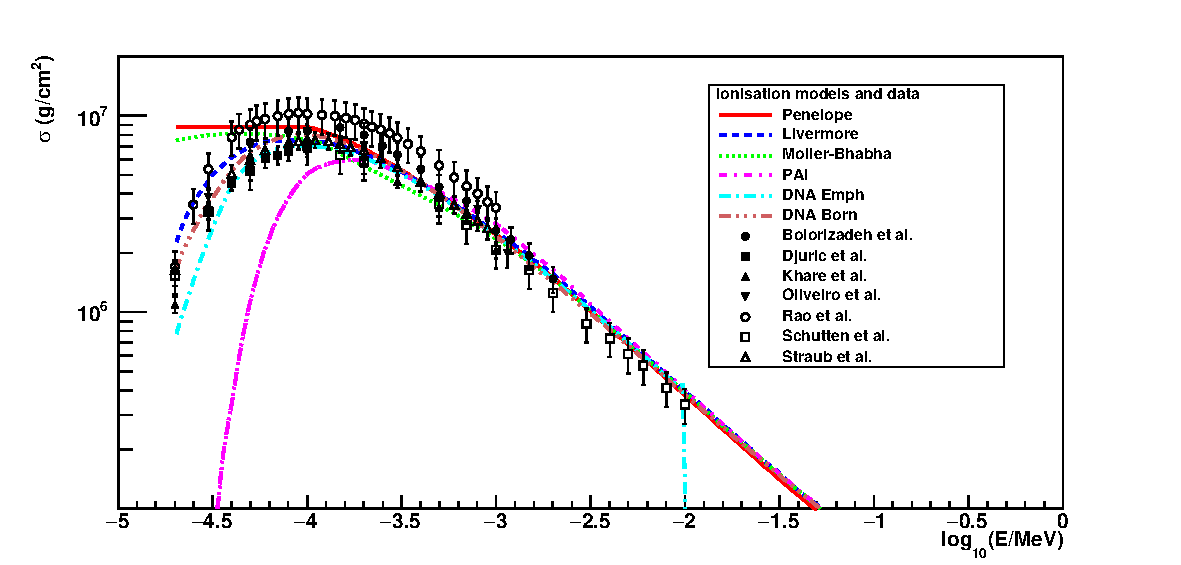
\includegraphics[width=3.8in]{figures/ApicXS_99.pdf}
\caption{Total cross section of delta electron production in liquid water as a
         function of projectile electron energy.  Curves correspond to different
         \Gfour{} ionization models, and points correspond to experimental data
         \cite{embib:dnaxs}.  The DNA model has an upper validity limit of
         1 MeV.}
\label{em:xsh2o}
\end{figure}

Recently, alternative ionization processes and models were introduced for
specific applications.  Contrary to the traditional condensed approach, these 
processes do not have a continuous energy loss component.  They explicitly 
generate all electrons down to very low energies.  They were first developed in
the framework of the \Gfour{}-DNA project (see \ref{sec:em9}), which aims to model
early biological damage induced by ionizing radiation at the DNA scale.  The 
\gclass{G4DNAIonisation} process has different models that apply to electrons, 
protons and selected ions (H, alpha, alpha+, He, Li, Be, B, C, N, O, Si and Fe)
in liquid water \cite{embib:dnaProc1, embib:dnaxs}.  Similarly, a specific
process, \gclass{G4MicroElecInelastic}, was developed for microelectronics 
applications, with a corresponding model that applies to electrons, protons and
heavy ions in silicon \cite{embib:micro, embib:micro1}.

Such models are applicable to a limited energy range and a selected set of 
materials, and in order to simulate realistic particle transport, it may be 
necessary to combine them with a continuous ionization process.  For this 
purpose the user may configure, for a given process and particle type,
several models for different energy ranges and detector regions \cite{bib:uni}.
These discrete models produce secondary electrons without the low energy 
threshold used by continuous ionization models, which could lead to 
discontinuous transitions between models.  To remedy this, the production of 
secondary electrons below the threshold may be enabled using the 
\gclass{G4VSubCutProsessor} interface, which works in parallel with the 
continuous model.

To illustrate this, cross sections of electrons in liquid water are shown in
Figure \ref{em:xsh2o}.  For the condensed approach models, a delta electron 
production threshold of 1 keV was used and the total electron cross section was
corrected for delta electron production below this threshold.



\subsubsection{Multiple and single scattering}\label{sec:em4} % JMCB Feedback
% Author: Omrane Kadri
%%%%%%%%%%%%%%%%%%%%%%%%%%%%%%%%%%%%%%%%%%%%%%%%%%%
% msc.tex
%%%%%%%%%%%%%%%%%%%%%%%%%%%%%%%%%%%%%%%%%%%%%%%%%%%
At present, the Monte Carlo simulation of charged particle transport in detailed
(interaction by interaction) mode is feasible only for projectiles with 
relatively low energies and for thin targets.  In general, the number of 
elastic interactions of a projectile before being stopped is very large and
detailed simulation becomes impractical.  The conventional solution for 
overcoming this difficulty is the implementation of condensed-history 
simulation schemes, in which the cumulative effect of many elastic scatterings
along a given track segment is simulated by using multiple scattering theories
such as Moli\`{e}re \cite{embib:msc2, embib:msc3}, Goudsmit and Saunderson
\cite{embib:msc4} and Lewis \cite{embib:msc6}.

\Gfour{} offers a diverse set of multiple scattering and single scattering
models \cite{embib:msc61,embib:msc1,embib:msc8,embib:msc9}.  Multiple scattering
models share the same \gclass{G4VMscModel} interface and were tuned per particle
type and application domain.  Recently, the possibility of sampling the lateral 
displacement of a charged particle at a geometry boundary was achieved by moving
the sampling of particle scattering from post-step to along-step, before 
sampling the energy loss and straggling.

Single scattering models sample each elastic collision of a charged particle, 
resulting in an increased number of steps and increased simulation time in 
comparison to multiple scattering models.  However, single scattering models 
have several important applications.  In particular, they are needed for the 
simulation of recoils \cite{embib:msc8,embib:msc9}, which is crucial, for 
example, for the understanding of single event effects in space electronics. 
Single scattering models are also needed to perform comparisons and validations
of multiple scattering models.  Single scattering models are useful for the 
sampling of charged particle transport in thin layers or low density media, and
in the vicinity of boundary crossing between two volumes.  In the majority of 
benchmark results for all particle types, single scattering predictions are 
closer to reference data than those of multiple scattering.

The choice of multiple scattering model strongly influences the CPU 
performance of the EM simulation.  The new unified design \cite{bib:uni} allows 
different multiple scattering models for different energy ranges to be used 
within the same simulation.  The analysis of all available results from multiple
scattering benchmarks \cite{embib:chep11,embib:msc1,embib:chep12} 
allows establishment of the optimal configuration of multiple and single 
scattering models in production physics lists.

In default physics lists, the Urban model is used below 100 MeV for electrons 
and positrons, where this model has a significant advantage in accuracy and 
CPU speed.  In the combined model \gclass{G4WentzelVIModel}, single scattering 
is applied only for hard scattering, which has a limited cross section, while
small angle scattering is sampled as multiple scattering \cite{embib:msc1}. 
The \gclass{G4WentzelVIModel} model provides results similar in accuracy to 
single scattering but it is much more computationally efficient.  As such, 
recent versions of \Gfour{} have this combined model set as the default for muon
and hadron transport, and for $e^{\pm}$ above 100 MeV.  Validation of multiple
scattering models for muons and hadrons are published elsewhere 
\cite{embib:chep14,embib:chep11,embib:msc1,embib:msc12}.

As an example of benchmark tests carried out, Figure~\ref{Figure-MSC1} 
illustrates the ratios of simulated to measured angular distribution widths
taken at the points where the distrubution falls to 1/e of the peak value.  The
measured data taken from literature \cite{embib:msc11} include a set of 
different target materials (Be, C, Al, Ti, Cu, Ta, Au) with an accuracy of about
1\%.  Using the \gclass{G4UrbanMscModel} of \Gfour{} release 10.0, the predicted 
angular distribution widths are close to the data with a maximum deviation not 
exceeding 3\% for both test cases of 13 and 20 MeV. 

\begin{figure}
\includegraphics[width=0.5\textwidth]{figures/ratio_13.pdf}
% \includegraphics[width=0.5\textwidth]{electromagnetic/ratio_13.eps}
\caption{The MC/data ratio of angular distribution widths measured at the 1/e
level for the Urban model of \Gfour{} 10.0.  Results are shown for a 13~MeV beam
on the target materials and thicknesses of the electron scattering benchmark
\cite{embib:msc11} .}
\label{Figure-MSC1}
\end{figure}




\subsubsection{Radiation of charged particles}\label{sec:em5}% JMCB Feedback
% Author: 
%%%%%%%%%%%%%%%%%%%%%%%%%%%%%%%%%%%%%%%%%%%%%%%%%%%
% brem.tex
%%%%%%%%%%%%%%%%%%%%%%%%%%%%%%%%%%%%%%%%%%%%%%%%%%%
A variety of models to simulate the radiation loss of charged particles are
available in the toolkit (Table~\ref{em:brem}).  Significant efforts were made
\cite{embib:chep12} to improve the description of EM shower shapes in order to
simulate accurate $H\to\gamma\gamma$ signals in the LHC detectors 
\cite{embib:Higgs1,embib:Higgs2}.  High energy EM shower profiles are sensitive 
to electron/positron bremsstrahlung spectra and angular distributions.
All \Gfour{} models of bremsstrahlung in the intermediate energy range 1~keV to
1~GeV are based on tables of differential cross sections published by Seltzer
and Berger \cite{embib:SelzBer}.  Evaluated 2-D tables are stored in the EM 
data set \gclass{G4LEDATA} and are loaded at initialization time.  The 
Ter-Mikaelian suppression of low energy gamma emission due to finite formation 
length (see \cite{embib:bremfl} and references therein) is taken into account 
by all models. 

\begin{table*}
\caption{List of \Gfour{} models for simulation of radiation loss with 
         recommended energy ranges. Array size refers to the internal table
         storing number of primary energy points versus number of secondary 
         energy points.}
\label{em:brem}
\begin{center}
\begin{tabular}{llll}
\hline
Particle& Model& Energy range&Array size \\ \hline
 e-/e+& \gclass{G4SeltzerBergerModel} \cite{embib:chep12}& 1 keV - 10 GeV & 57x32\\
 e-/e+ & \gclass{G4PenelopeBremsstrahlungModel} & 1 keV - 10 GeV & 57x32\\
e-  & \gclass{G4LivermoreBremsstrahlungModel} & 1 keV - 10 GeV & 31x14 \\
 e-/e+ & \gclass{G4eBremsstrahlungRelModel} \cite{embib:chep12}&   1 GeV - 10 PeV &  \\
$\mu^{\pm}$    & \gclass{G4MuBremsstrahlungModel} \cite{embib:emmu}& 1 GeV - 10 PeV & \\
$\mu^{\pm}$    & \gclass{G4MuPairProductionModel} \cite{embib:emmu}& 1 GeV - 10 PeV & 17x1000\\
$\pi^{\pm}, K^{\pm}, p$ &\gclass{G4hBremsstrahlungModel} \cite{embib:hb}&5 GeV - 10 PeV &\\
$\pi^{\pm}, K^{\pm}, p$ &\gclass{G4hPairProductionModel} \cite{embib:hb}&5 GeV - 10 PeV &13x1000 \\
\hline
\end{tabular}
\end{center}
\end{table*}
For $e^{\pm}$ above 1~GeV, a relativistic model \cite{embib:chep12} was developed
with an improved treatment of the LPM effect \cite{embib:migdal}.  This was 
implemented on top of the classical Bethe-Heitler cross section with complete 
screening.  Two types of saturation effects, LPM and formation length, have been 
combined to limit the number of low energy photons produced.  These corrections
have a distinct impact on EM shower shape and fluctuations of energy loss for
high energy EM particles, of particular importance in LHC experiments.

Because simulation of radiation losses of muons is also important for LHC 
experiments, muon bremsstrahlung and pair production models were developed
\cite{embib:emmu}.  The effect of catastrophic energy loss by high energy muon 
bremsstrahlung is well reproduced by simulation and is essential for muon 
identification.  The process of $e^+e^-$ pair production by muons dominates the
average energy loss at high energy \cite{embib:emmu}; proper simulation of the 
final state requires keeping a detailed 2-D internal table of differential cross
sections (Table~\ref{em:brem}) with a structure chosen to achieve a compromise 
between memory usage, initialization time, and accuracy \cite{embib:chep14}.  
Analysis of CMS test beam data \cite{embib:cmstb} indicates that bremsstrahlung
and pair production by pions and protons should be taken into account.  This was
achieved on top of the muon processes by changing the spin term and the mass of 
projectile particles \cite{embib:hb}. 


\subsubsection{Polarization models}\label{sec:em6} % JMCB Feedback
% Author: Paul Gueye
%%%%%%%%%%%%%%%%%%%%%%%%%%%%%%%%%%%%%%%%%%%%%%%%%%%
% polar.tex
%%%%%%%%%%%%%%%%%%%%%%%%%%%%%%%%%%%%%%%%%%%%%%%%%%%
Models for the simulation of linear polarized gamma transport are based 
on the set of Livermore gamma models: photoelectric effect \cite{embib:gamma9}, 
Rayleigh and Compton scattering \cite{embib:gamma10}, and gamma conversion. 
These models have been part of \Gfour{} for a long time.  New gamma conversion
models briefly described in Section \ref{sec:em2} also take into account linear
polarization of a primary gamma.  Also the process of positron annihilation was
updated, and now takes into account the correlation of photon polarization in 
the annihilation rest frame.

In parallel, a polarization sub-library was designed to use the standard 
gamma models \cite{embib:pol5}.  This library allows for the simulation of 
circularly polarized electrons and positrons in vacuum and in polarized media.
For a complete simulation of a low energy polarimeter setup, all processes
relevant to tracking polarized particles through matter, such as spin-dependent
Compton scattering, Bhabha-M\"{o}ller scattering, annihilation, bremsstrahlung
and pair production, were implemented.  The main application of this library is
in the design of positron sources for future linear colliders \cite{embib:pol6}.


\subsubsection{High energy models}\label{sec:em61} % JMCB Feedback 
% Author: 
%%%%%%%%%%%%%%%%%%%%%%%%%%%%%%%%%%%%%%%%%%%%%%%%%%%
% high.tex
%%%%%%%%%%%%%%%%%%%%%%%%%%%%%%%%%%%%%%%%%%%%%%%%%%%
% For specific studies at the LHC and design of future linear colliders 
% \cite{embib:lin}, a set of high energy models have been developed. 
The processes of gamma conversion to muon pairs \cite{embib:gmumu}, and positron
annihilation into muons and hadrons \cite{embib:emmu}, were implemented to assist
in the design of interaction regions within future linear colliders
\cite{embib:lind}.  Other models were added for the simulation of energy loss of
heavy exotic particles, in particular, magnetic monopoles \cite{embib:empbar}. 
Because the charges and masses of these objects are not always defined, the new 
models allow for the flexible definition of the energy ranges over which they
are valid, and are not constrained by the lower or upper limits seen in Table
\ref{Table-Ioni}.  An efficient generator for synchrotron radiation by 
relativistic electrons in magnetic fields was also implemented \cite{embib:syn}
and recently generalized to synchrotron radiation for any type of long-lived 
charged particle.



\subsubsection{Atomic de-excitation}\label{sec:em7} % JMCB Feedback 
% Author: 
%%%%%%%%%%%%%%%%%%%%%%%%%%%%%%%%%%%%%%%%%%%%%%%%%%%
% deex.tex
%%%%%%%%%%%%%%%%%%%%%%%%%%%%%%%%%%%%%%%%%%%%%%%%%%%

Atomic de-excitation can be activated in all EM physics lists through the common
atomic de-excitation interface \gclass{G4VAtomDeexcitation} \cite{bib:uni}.
Photo-electric effect, Compton scattering, and discrete ionization models 
provide cross sections of ionization for each atomic shell.  The de-excitation
code is responsible for sampling the electromagnetic cascade with fluorescence
and Auger electron emission, and was implemented using evaluated data 
\cite{embib:eadl}. Recently, alternative, more accurate transition energies have
become available in \Gfour{} 10.1 through the addition of a new data set 
\cite{embib:SPaltani}.

The ionization cross section model for Particle Induced X-ray Emission (PIXE) is
based on the condensed history approach.  Specific cross sections can be defined
for electrons, protons, and ions.  Users can select from different sets of 
theoretical or empirical shell ionization cross sections \cite{embib:pixe}.

The simulation of K, L, and M X-ray yields demands knowledge of the X-ray 
production cross sections.  These were calculated using the ECPSSR theory, 
initially developed by Brandt and Lapicki \cite{embib:deex1} and recently 
reviewed \cite{embib:deex2,embib:deex3}.  Computing the X-ray production cross 
sections from first principles is a time-consuming process due to the numerical 
double integral of form factor functions needed to obtain the ionization cross 
sections for each shell or sub-shell (Eq.(23) of \cite{embib:deex2}), over all 
possible values of the energy and momentum transfer of the incident particle.  

The calculation was expedited through the use either of extensive tables and
interpolation methods, or efficient algorithms providing sufficiently good
approximations.
% Aside from empirical tabulations data and a full analytical
% calculations method, efficient algorithms were implemented to determine K, L 
% and M-shells ionization cross-sections
% for H and He ions. 
Algorithms were implemented based on the ECPSSR ionization cross sections for
H and He ions calculated for the K and L shells using the form factor functions
for elements with atomic number 6 to 92 over the energy range of 0.1 to 100 
MeV.  In the case of the M shells, the ionization cross sections are given 
for elements with atomic number 62 to 92 over the energy range of 0.1 to 10 MeV.
Furthermore, the tables generated to develop the algorithms were obtained by
the integration of the form factor functions that describe the process using 
Lobatto's rule \cite{embib:deex4}, and are also available.  The cross sections
generated by the algorithms deviate less than 3\% from the tabulated values, 
roughly matching the scatter of empirical data \cite{embib:deex2}.  Further 
details and considerations of these calculations can be found in 
\cite{embib:deex2,embib:deex3}.  Comparisons of simulated and experimental 
spectra obtained under proton irradiation of several materials are shown in
\cite{embib:deex5,embib:deex6}.



\subsubsection{Optical physics}\label{sec:em8} % JMCB Feedback 
% Author: Peter Gumplinger
%%%%%%%%%%%%%%%%%%%%%%%%%%%%%%%%%%%%%%%%%%%%%%%%%%%
% xray_opt.tex
%%%%%%%%%%%%%%%%%%%%%%%%%%%%%%%%%%%%%%%%%%%%%%%%%%%
\Gfour{} can accurately simulate nonlinear scintillators where the light yield is
a function of particle type, energy deposition and kinetic energy of the 
ionizing particle \cite{em:opt1}.  In scintillators with a linear response, 
light production is directly proportional to the ionizing energy deposited and
the total light produced can be computed as the sum of the light produced during
small simulation steps without regard for the kinetic energy of the ionizing 
particle at each energy-depositing step.

In scintillators with a nonlinear response, the yield during a step is
calculated as the difference in yields for hypothetical, totally absorbed 
particles at the kinetic energies before and after the step.  This method 
correctly models the total light produced by a multiple step ionizing particle 
track, and accounts for two important cases.  In the first case, light is 
produced correctly for incomplete energy deposition of a charged particle, such
as when the particle exits the scintillator volume or when the particle is 
absorbed in a nuclear reaction.  In the second case, the scintillation photon 
density is larger in the high kinetic energy portion of the track for the usual
case where the nonlinear photon yield increases with particle energy.  This 
enables the precision simulation of organic or noble gas scintillators, provided
the user supplies the required data inputs.

Two more refinements in the generation of optical photons are that the 
scintillation process takes into account a finite light emission rise-time, 
and that the Cerenkov photon origin density along the track segment is no longer 
constant, but assumes a linear decrease in the mean number of photons generated 
over the step as the radiating particle slows down.

For the propagation of optical photons, the reflectivity from a metal surface
may now be calculated by using a complex index of refraction \cite{embib:Iowa}.
%\footnote{Thanks to Sehwook Lee and John Hauptman (Iowa State 
%University)} 
Mie scattering was added following the \mbox{Henyey-Greenstein} approximation, 
with the forward and backward angles treated separately \cite{embib:Mie}.
% \footnote{Thanks to Xin Qian (Caltech) based on work from Vlasios 
% Vasileiou (University of Maryland)} 
Surface reflections may be simulated using look-up tables containing measured
optical reflectance for a variety of surface treatments \cite{em:opt2}. It is 
possible to define anti-reflective coatings, and transmission of a dichroic 
filter where the transmission, or conversely the reflection, is dependent on 
wavelength and incident angle.  The optical boundary process also works in 
situations where the surface is between two volumes, each defined in a different
parallel world, thus allowing optical photon propagation for previously 
impossible geometry implementations.

%end


\subsubsection{\Gfour{}-DNA physics models}\label{sec:em9} % JMCB Feedback 
% Author: Sebastien Incerti
%%%%%%%%%%%%%%%%%%%%%%%%%%%%%%%%%%%%%%%%%%%%%%%%%%%
% dna.tex
%%%%%%%%%%%%%%%%%%%%%%%%%%%%%%%%%%%%%%%%%%%%%%%%%%%
\Gfour{} offers a set of physics processes and models \cite{embib:dna0} to 
simulate track structure in liquid water, the main component of biological
media.  These were developed as part of the \Gfour{}-DNA project 
\cite{embib:dnaweb}, and extend  
% in 2001 by the European 
% Space Agency 
\Gfour{} to include the simulation of biological damage by ionizing radiation
\cite{embib:dna1,embib:dna2}. 

The first set of discrete processes was delivered in 2007 \cite{embib:dnaProc1}.
Their accuracy was further evaluated and improved 
\cite{embib:dnaxs, embib:dnaProc2, embib:dnaProc3} through the inclusion, 
for example, of more accurate modeling of electron elastic scattering
\cite{embib:dnaElast}, and additional physical processes for sub-excitation
electrons, such as vibrational excitation and molecular attachment 
\cite{embib:dnaTS}.  These processes are critical for the modeling of
physico-chemical processes in liquid water \cite{embib:chem:paper1}. 

A major design upgrade of the software classes was applied in order to allow 
their combination with other \Gfour{} EM processes and models, for a coherent 
modeling of EM interactions \cite{bib:uni,embib:dnaPhysList}.  Thus, for 
their simulation applications, users may instantiate a 
\gclass{G4EmDNA\allowbreak{}Physics} object from their physics list.  This 
physics constructor contains all required \Gfour{}-DNA physics processes and 
models for
\begin{itemize} 
\item electrons, including ionization, excitation, elastic scattering, 
      vibrational excitation and attachment,
\item protons and neutral hydrogen, including excitation, ionization, electron
      capture and stripping,
\item alpha particles and their charged states, including excitation,
      ionization, electron capture and stripping, and  
\item ionization for Li, Be, B, C, N, O, Si and Fe ions.
\end{itemize}
 
Stopping powers and ranges simulated with \Gfour{}-DNA have been compared to
international recommendations \cite{embib:dnaStop}.  These processes can be
combined with \Gfour{} gamma processes.  Note that the \emph{Livermore} low
energy electromagnetic gamma models are selected by default in the 
\gclass{G4EmDNA\allowbreak{}Physics} constructor. 

As an illustration, \\
\verb"examples/extended/medical/dna/dnaphysics"\\
explains how to use this physics constructor.  In addition,
\verb"examples/extended/medical/dna/microdosimetry" describes how to 
combine \Gfour{}-DNA and \Gfour{} standard electromagnetic processes in a simple
user application.  A variety of applications based on \Gfour{}-DNA processes and
models allow the study of elementary energy deposition patterns at the 
sub-cellular scale.  For example, the comparison of dose point kernels 
\cite{embib:dnaPK}, $S$-values  \cite{embib:dnaS}, radial doses 
\cite{embib:dnaRad}, cluster patterns for ions with the same LET 
\cite{embib:dnaLET}, the effect of a magnetic field on electron track structures
\cite{embib:dnaMag}, and the modeling of direct DNA damage 
\cite{embib:dnaDirD1,embib:dnaDirD2,embib:dnaDirD3,embib:dnaDirD4}
have so far been explored utilizing these tools.  They even provide a framework
for the future study of non-targeted biological effects \cite{embib:dnaBio}, 
extending further the first applications of \Gfour{} electromagnetic physics at 
the physics-biology frontier
\cite{embib:dnaBio1,embib:dnaBio2,embib:dnaBio3,embib:dnaBio4,embib:dnaBio6,embib:dnaBio7,embib:dnaBio8}.



\subsubsection{\Gfour{}-DNA physico-chemistry module}\label{sec:em10} % JMCB Feedback 
% Author: Mathieu Karamitros
%%%%%%%%%%%%%%%%%%%%%%%%%%%%%%%%%%%%%%%%%%%%%%%%%%%
% chem.tex
%%%%%%%%%%%%%%%%%%%%%%%%%%%%%%%%%%%%%%%%%%%%%%%%%%%

Radiation chemistry is the science of the chemical effects of radiation on
matter.  Simulation tools in this field are relevant to many applications, such
as the production of polymers by the irradiation of monomers.  However, one of
the most studied materials under irradiation is liquid water, because it is used
as a coolant in nuclear power plants and its irradiation may create oxidative 
species that are likely to initiate the corrosion process.  Water is also of 
interest because it is the main component of biological materials.

When biological targets are exposed to radiation, the chemical response can be 
complex, depending on the composition of the medium as well as on the energy and
type of radiation.  For example, water radiolysis (dissociation of water by 
radiation) promotes the creation of oxidative species.  These species can either
react with one another or with the biological materials, interfering with the 
normal functioning of one or many cells.

In the context of the \Gfour{}-DNA project, a prototype for simulating radiation 
chemistry was developed \cite{embib:dna3, embib:chem:paper1} and delivered with
\Gfour{} version 10.1.  It is now possible to simulate the physical stage, the 
physico-chemical stage (lasting up to about 1 picosecond) and the chemical stage
(from 1 picosecond up to 1 microsecond) of water radiolysis.
%   The simulation proceeds in two stages, the first 
% consisting of prompt physics processes (reaction times $ < 10^{-9} s$) which 
% provide a set of wounded biological and water molecules in a volume of interest, 
% and the second consisting of physico-chemical processes with reaction times up
% to $10^{-6} s$. 

The \Gfour{}-DNA physical processes may in some cases create
water molecules which are electronically modified, that is, they may be ionized,
excited or have extra electrons in the case of dissociative attachment.  The 
electronic and atomic readjustment of the water molecules can eventually lead to
their dissociation.  The dissociation of water molecules is taken into account 
by random selection using user-defined branching ratios \cite{embib:chem:paper1}.
The positioning of the dissociative products is defined by the 
\gclass{G4DNAWater\allowbreak{}DissociationDisplacer} class from qualitative 
considerations \cite{embib:chem:Kreipl2009}.  It is assumed that the 
dissociation of water molecules is independent of the physical stage of the 
simulation.  This is to say that only electronic modifications undergone by the
water molecule are responsible for the dissociative pathways.  The branching 
ratios and positioning of dissociative products may be adjusted by the user if 
necessary.

Dissociative products can recombine to form new chemical species. To take this 
recombination into account, a stepping algorithm was developed specifically for 
managing collisions between \Gfour{} tracks.  The purpose of this algorithm is 
to synchronize the transport of tracks during simulation.  This means that all 
tracks are transported over the same time, accounting for chemical reactions 
that may happen during a given time step. A description of this synchronized 
stepping, applied to radiation chemistry, is available 
in \cite{embib:dna3,embib:chem:these}.

This stepping mechanism could, in principle, be applied to applications other
than radiation chemistry.  A process must first be made compatible with the 
\gclass{G4VITProcess} interface, which contains track information.  To run a 
radio-chemistry simulation, a table of reactions describing the supported 
reactions and the corresponding reaction rates must be provided.

To simplify the use of the chemistry module, the 
\gclass{G4EmDNA\allowbreak{}Chemistry} constructor provides default settings,
and three examples, 
\verb"examples/extended/medical/dna/chem1", 
\verb"examples/extended/medical/dna/chem2" and
\verb"examples/extended/medical/dna/chem3", are included.  These examples 
progressively demonstrate how to activate and use the chemistry module from a
user application. The module may be used with or without irradiation.

The chemistry module is compatible with the current event-level multithreaded 
mode of \Gfour{}.  However, the use of the module in this mode with a large number
of simulated objects or threads is not recommended because synchronized stepping
requires intense memory usage.

For now, the chemistry module allows prediction of the chemical kinetics induced 
by ionizing radiation. A future goal of the \Gfour{}-DNA project is to account for
DNA damage resulting from irradiation. 


% % \subsubsection{Physics Lists}\label{sec:em11} % JMCB Feedback 
% % Author: 
% % %%%%%%%%%%%%%%%%%%%%%%%%%%%%%%%%%%%%%%%%%%%%%%%%%%%
% phys.tex
%%%%%%%%%%%%%%%%%%%%%%%%%%%%%%%%%%%%%%%%%%%%%%%%%%%
%Many years of experience with Geant4 across a large number of applications 
%has demonstrated the significant advantage of a modular physics lists approach, 
%where each type of physics is instantiated by a \emph{physics constructor} 
%class. Geant4 maintains several EM constructors (Table~\ref{em:physl}) which 
%are created for different application domains. These constructor classes are 
%components of full Geant4 reference physics lists 
%(for example, $FTFP\_BERT$, $FTFP\_BIC\_EMY$...), and are available for EM 
%production physics constructors (names are defined in Table~\ref{em:physl}). 
%At the same time, all EM constructors may be directly used by custom 
%physics lists.

%The physics of a \Gfour\ simulation is built in a modular approach, in which a
%list (called a physics list) of interaction types is created. 

Electromagnetic physics is defined in physics constructor classes, which are
components of full physics classes. \Gfour{} maintains several EM constructors
(Table~\ref{em:physl}) for different application domains. The constructors are 
used by both \Gfour{} reference physics lists and custom physics lists.

For HEP experiments, high efficiency CPU performance is required, and, as 
such, the HEP physics configuration should provide a compromise between 
accuracy and CPU speed. For simulation of shielding in space and for radiation 
dose in medical studies, more detailed tracking of low energy particles is 
required. For this purpose, in physics constructors oriented towards medicine 
and space science applications 
(i.e. \gclass{G4EmStandardPhysics\_option4}, named $EMZ$), more strong step 
limitation are defined and models with more detailed treatment of atomic 
effects and detailed ion stopping powers are applied. A general goal is to 
provide a physics constructor with set of the most accurate models for each 
energy range and particle type.

To assist in the production and testing of physics constructors, 
experimental constructors are available. 
\Gfour{}-DNA physics constructors are applicable only 
for a limited set of materials (mainly liquid water). Examples 
of how to build physics lists with \Gfour{}-DNA physics, low energy, 
and standard 
physics \cite{embib:uni} are distributed with \Gfour{}. Specific physics 
constructors are provided for optical physics which can be added 
on top of any existing physics list.

\begin{table*}
\caption{List of \Gfour{} EM physics constructors}
\label{em:physl}
\begin{center}
\begin{tabular}{llll}
\hline
Constructor& Application& Name & Comment \\ \hline
\gclass{G4EmStandardPhysics} & HEP &  &default (ATLAS)\\
\gclass{G4EmStandardPhysics_option1} & & EMV & simplified (CMS)\\
\gclass{G4EmStandardPhysics_option2} & & EMX & simplified (LHCb)\\
\hline
\gclass{G4EmStandardPhysics_option3} & space \& & EMY & detailed  \\
                             &  medicine &     & standard models\\
\gclass{G4EmLivermorePhysics} & & LIV & detailed  \\
                     &       &          &  Livermore models\\
\gclass{G4EmPenelopePhysics} &  & PEN & detailed \\ 
                    &  &     & Penelope models\\
\gclass{G4EmStandardPhysics_option4} &  & EMZ & combining \\
                             &  &     & best models\\
\hline
\gclass{G4EmLivermorePolarizedPhysics} &  &  & polarized models\\
\gclass{G4EmLowEPPhysics} &  &  & new low energy models\\
\gclass{G4EmStandardPhysicsWVI} &  &  & WVI multiple scattering\\
\gclass{G4EmStandardPhysicsSS} &  &  & single scattering \\
\hline
\gclass{G4EmDNAPhysics} & DNA &  & default for DNA physics \\
\gclass{G4EmDNAPhysics_option1} & DNA &  & WVI multiple scattering \\
\hline
\gclass{G4OpticalPhysics} & all &  & production and transport \\
                 &     &  & of optical photons \\
\hline
\end{tabular}
\end{center}
\end{table*}


\subsubsection{Built-in EM biasing options}\label{sec:em12} % JMCB Feedback
% Author: Daren Sawkey
%%%%%%%%%%%%%%%%%%%%%%%%%%%%%%%%%%%%%%%%%%%%%%%%%%%
% bias.tex
%%%%%%%%%%%%%%%%%%%%%%%%%%%%%%%%%%%%%%%%%%%%%%%%%%%
Four biasing and variance reduction options are available within the EM
sub-libraries of \Gfour{} \cite{embib:uni2}: 
\begin{itemize}
\item cross section biasing, which may be used to study the effects of 
      uncertainties of cross sections;
\item forced interaction, implemented for the limited use-case of a thin target; 
\item splitting, where the interaction of a primary of weight $W$ which would 
      normally produce 1 secondary of weight $W$, instead produces $N$ secondaries,
      each with weight $W/N$, with no modification of the energy of the primary;
\item Russian roulette, where secondaries produced by the interaction of a
      primary particle of weight $W$ are killed with probability $1 - P$, and
      the survivors' weight is set to $W/P$; users may define $P$ and the upper 
      energy limit for secondaries for which the method is applied.
\end{itemize}

These four options are selectable through macro commands or C++ interfaces, 
and can be applied in user-defined \gclass{G4Region}s.


\subsubsection{Validation and verification of EM models}\label{sec:em13}
% Author: Vladimir Ivanchenko
%%%%%%%%%%%%%%%%%%%%%%%%%%%%%%%%%%%%%%%%%%%%%%%%%%%
% val.tex
%%%%%%%%%%%%%%%%%%%%%%%%%%%%%%%%%%%%%%%%%%%%%%%%%%%
Validation of EM physics is performed on several levels.  Because EM physics is
used in practically all tests and examples, the \Gfour{} integrated test system 
routinely checks all EM physics models.  A specific EM validation suite
\cite{embib:emVal} runs on a regular basis for each reference version of \Gfour{}
(see \cite{embib:chep14,embib:chep11,embib:chep12} and references therein).
Dedicated validations of cross sections, stopping powers, and atomic transition
energies versus evaluated data and theory are done by \Gfour{} developers and 
different user groups (see, for example, 
\cite{embib:uni2,embib:valGam,embib:valGam2} and 
Figure \ref{em:compton}).  EM physics validation is also performed in various
application domains by different user communities, especially by the HEP 
experiments ATLAS and CMS. 

As an example of EM physics validation for HEP applications, the energy 
resolution of two sampling calorimeters \cite{embib:uni3,embib:uni4} 
versus the cut in range value and \Gfour{} version is shown in 
Figure~\ref{Figure-UEM1}.  This plot illustrates the good agreement of \Gfour{}
simulation predictions with data, and the stability between \Gfour{} versions of 
simulation results for high energy physics applications.

\begin{figure}
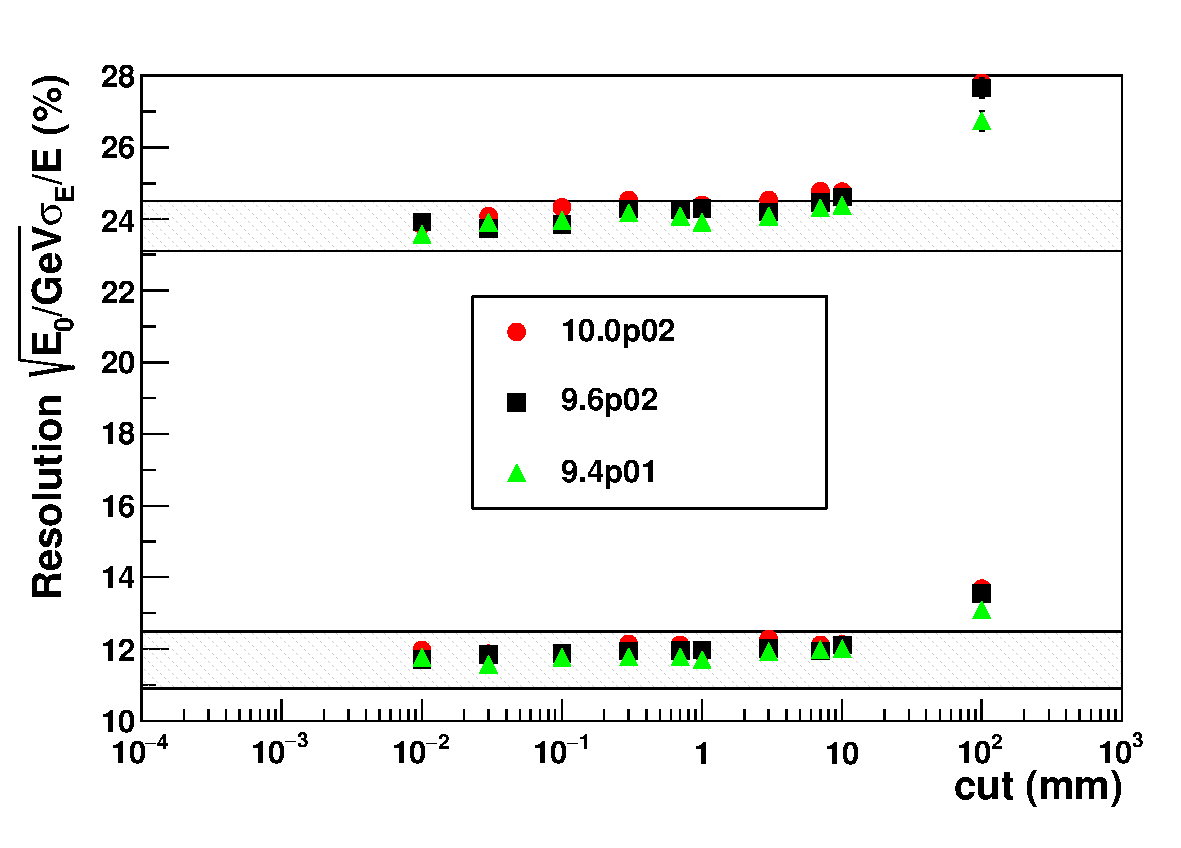
\includegraphics[width=0.5\textwidth]{figures/Azeus.pdf}
\caption{Energy resolution of two sampling Lead/Scintillator calorimeters 
for 10 GeV electrons: squares, circles and triangles indicate \Gfour{} 
simulations for different versions of the toolkit, and each band indicates 
experimental data with one standard deviation uncertainty
\cite{embib:uni3,embib:uni4}.}
\label{Figure-UEM1}
\end{figure}

Further validations come from the medical and space communities, in particular, 
GATE \cite{embib:GATE}, GAMOS \cite{embib:GAMOS}, GRAS \cite{embib:gras}, 
and TOPAS \cite{embib:TOPAS}.
There are also many validation results obtained by single user groups.  For 
example, validations for space shielding were done recently in 
\cite{embib:elshield} and for therapeutic ion beam simulation in 
\cite{embib:emIonUser}.

%end


%end


  
\subsection{\textbf{Hadronic physics}}\label{sec:hadphys}
\Gfour{} hadronic physics is loosely defined to cover any reaction which can
produce hadrons in its final state.  As such, it covers purely hadronic
interactions, lepton- and gamma-induced nuclear reactions, and radioactive
decay.  The interaction is represented as a \Gfour{} process which consists of
a cross section to determine when the interaction will occur, and a model which
determines the final state of the interaction.    

Models and cross sections are provided which span an energy range from sub-eV to
~TeV.  Following the toolkit philosophy, more than one model or process is 
usually offered in any given energy range in order to provide alternative 
approaches for different applications. 

During the last several years, new models and cross sections have been added
to the toolkit, while others have been improved and some obsolete models have
been removed.

% shortcut commands for some model names
\newcommand{\incl}{INCL}
\newcommand{\inclxx}{INCL++}
\newcommand{\abla}{ABLA~V3}

%------------------------ Uzhi part ----------------------------------
% A simulation of a particle propagation in a matter requires the following steps:
% a choice of an interaction point and a target nucleus which depend on cross sections
% of the particle interactions with components of the matter, a sampling of a reaction
% of the particle with chosen target nucleus and a simulation of the reaction.
%---------------- Uzhi changes -----------------------------------

\subsubsection{Hadronic cross sections}\label{sec:crosssections}
Total, inelastic and elastic cross sections for hadron-nucleus, nucleus-nucleus
and antinucleus-nucleus reactions are provided which cover energies up to ~TeV 
in some cases.  Proton-, neutron- and pion-nucleus cross sections at low to 
medium energies have been available in \Gfour{} since its beginning and their 
details are covered elsewhere \cite{bib:generalpaper2}.  The focus here is on 
recent developments in cross sections for other projectile types and at higher
energies. \\

% done
%%%%%%%%%%%%%%%%%%%%%%%%%%%%%%%%%%%%%%%%%%%%%%%%%%%
% barashenkov.tex
% Author: Vladimir Grichine
%%%%%%%%%%%%%%%%%%%%%%%%%%%%%%%%%%%%%%%%%%%%%%%%%%%
% \noindent {\emph{Barashenkov cross sections}}
\paragraph{Barashenkov cross sections}
The Barashenkov data set describes proton, neutron and charged pion cross 
sections (total and inelastic) on nuclei~\cite{hadbib:bar90,hadbib:bar89}. 
The Barashenkov interpolation for the total and inelastic cross sections is
essentially based on a quasi-optical model for high energies (T$\,\,>\,\,$2 GeV)
and on phenomenology, with correction terms of the form $\pi r_o A^{2/3}$, 
with $r_o\sim\,\,$1 fm.  The total, inelastic (and elastic) cross sections were
modeled with:
\[
\sigma(T,A)=\pi \left[r_{o}A^{1/3}+\lambda(T,A)\right]^{2}f(T)\phi(A)^{\alpha(T)},
\]
where $\lambda$ is the de Broglie length of the projectile in the center of 
mass system, $T$ is the kinetic energy of the projectile in the lab, $A$ is the 
atomic weight and $r_{o}\sim 1\,\,$fm. 
The functions $f(T)$, $\phi(A)$ and $\alpha(T)$ are series of the form:
\[
\sum_i a_i T^{b_i}\quad\textrm{or}\quad \sum_i a_i A^{b_i}.
\]
The general behavior of the optical models is to predict constant cross sections
for very high energies.  However, experimental data show a moderate relativistic 
rise of hadron-nucleus cross sections.  For this reason the Glauber model was
used to describe hadron-nucleus cross sections in the high energy region (above
90 GeV).


% done
%%%%%%%%%%%%%%%%%%%%%%%%%%%%%%%%%%%%%%%%%%%%%%%%%%%
% glaubergribov.tex
% Author: Gunter Folger, Vladimir Grichine
%%%%%%%%%%%%%%%%%%%%%%%%%%%%%%%%%%%%%%%%%%%%%%%%%%%
\paragraph{Glauber-Gribov extension}
The simplified Glauber model cross sections assume Gaussian-distributed,
point-like nucleons and are given by~\cite{hadbib:ggepjc,hadbib:ggnimb}:
\[
\sigma^{hA}_{tot}=2\pi R^2\ln\left[1+\frac{A\sigma^{hN}_{tot}}{2\pi R^2}\right],\quad
\sigma^{hA}_{in} = \pi R^2\ln\left[1+\frac{A\sigma^{hN}_{tot}}{\pi R^2}\right],
\]
\[
\quad \sigma^{hA}_{el}=\sigma^{hA}_{tot}-\sigma^{hA}_{in}.
\]
Here $\sigma^{hA}_{tot}$, $\sigma^{hA}_{in}$, and $\sigma^{hA}_{el}$ are the
total, inelastic and elastic cross sections, respectively. 

The model is reduced to the selection of $\sigma^{hN}_{tot}$ and $R(A)$
values.  The latest edition of PDG \cite{hadbib:PDG} and \Gfour{} parameterizations
were used for $\sigma^{hN}_{tot}$, including the total cross sections of $p$,
$\bar{p}$, $n$, $\pi^{\pm}$, $K^{\pm}$ and $\Sigma^{-}$ on protons and neutrons
% (http://pdg.lbl.gov/2006/reviews/hadronicrpp.pdf).  
For known cross sections on protons and neutrons,
$A\sigma^{hN}_{tot}=N_{p}\sigma^{hp}_{tot}+N_{n}\sigma^{hn}_{tot}$, where $N_{p}$
and $N_{n}$ are the number of protons and neutrons in the nucleus.
The nuclear radius (the RMS radius of the nucleon Gaussian distribution), 
is parametrized as $R(A) = r_{o}A^{\frac{1}{3}}f(A)$, 
$r_{o} \sim 1.1 \ fm$, with $f(A) < 1$ for $A > 21$, and $f(A) > 1$ for the  
case $3 < A < 21$. 
Figures \ref{nCtotinprodGG} and \ref{pCinprodBGG} show the prediction of the
Barashenkov and Glauber-Gribov model for total, inelastic and production cross
sections of neutrons and protons on a carbon target.  The production cross
section is defined to be the difference between the inelastic and charge 
exchange cross sections.  

\begin{figure}
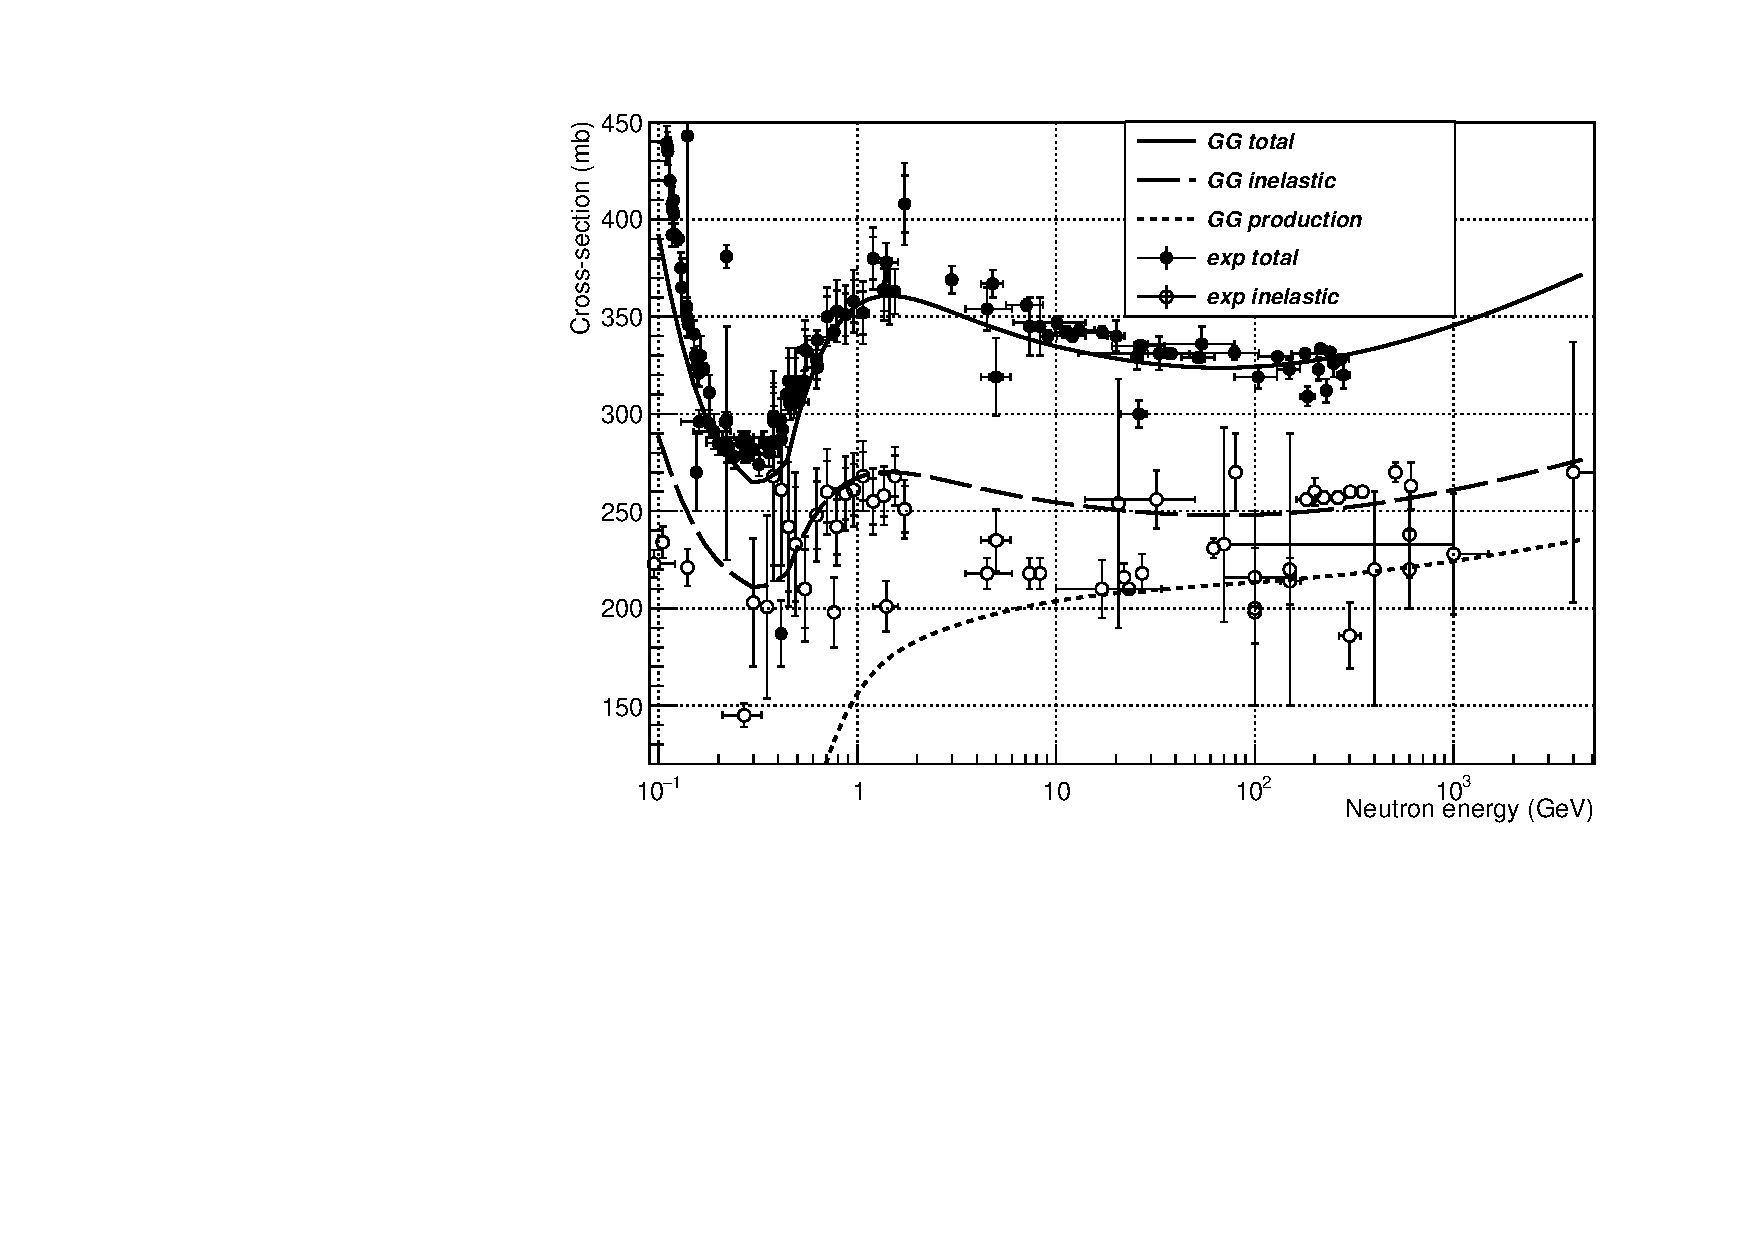
\includegraphics[width=0.5\textwidth]{figures/nCtotinprodGG.pdf}
% \centering \includegraphics[height=3.3in,width=3.6in]{figures/nCtotinprodGG.eps}
\caption{ Total, inelastic and production cross-sections of neutrons on a carbon 
target in the energy range $10^{-2}-10^3$~GeV. Experimental data (open and solid
points) from \cite{hadbib:ihepbase,hadbib:dubnabase}, lines correspond to the 
Glauber-Gribov model.}
\label{nCtotinprodGG}
\end{figure}

\begin{figure}
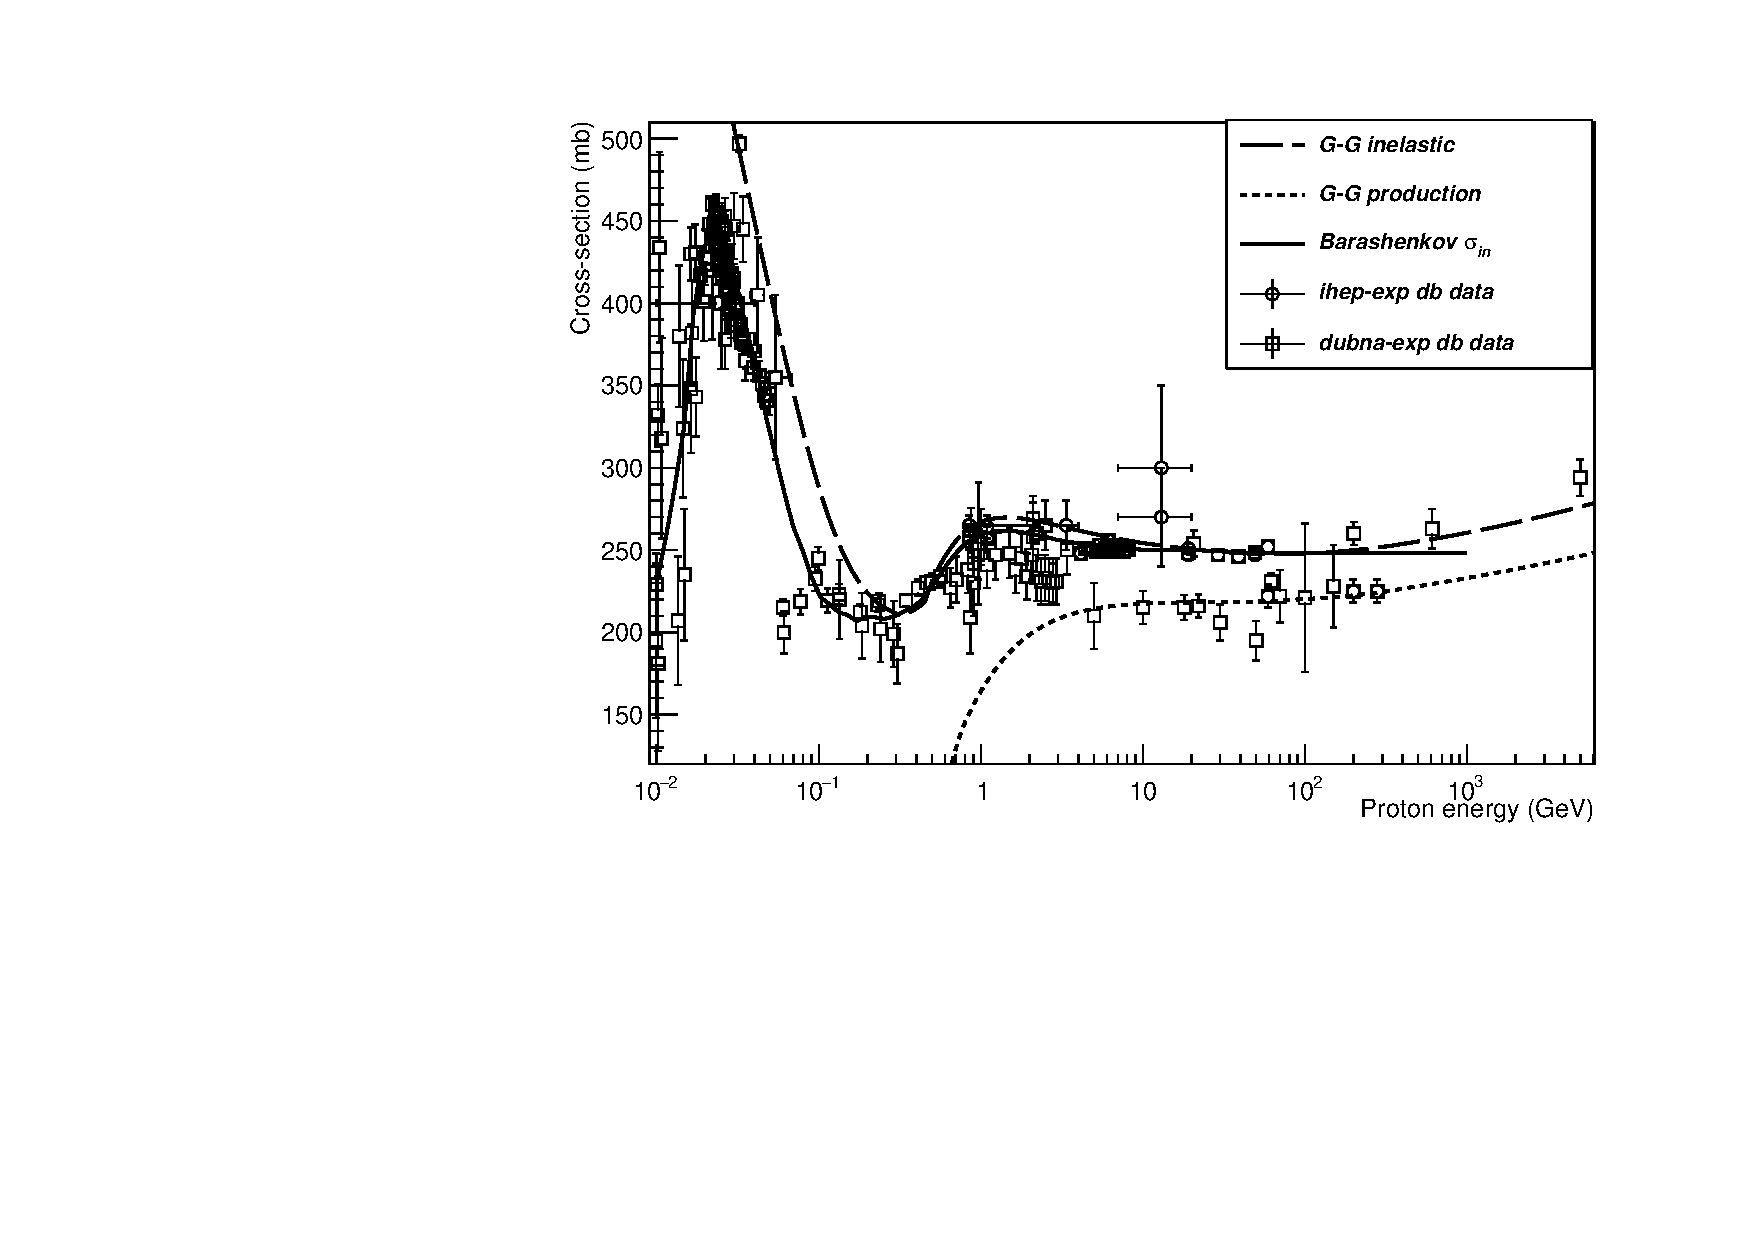
\includegraphics[width=0.5\textwidth]{figures/pCinprodBGG.pdf}
% \centering \includegraphics[height=3.3in,width=3.6in]{figures/pCinprodBGG.eps}
\caption{ Inelastic and production cross-sections of protons on a carbon 
target in the energy range $10^{-2}-10^3$~GeV. Experimental data (open points
and squares) are from \cite{hadbib:ihepbase,hadbib:dubnabase}. The solid and 
dashed lines correspond to the Barashenkov and Glauber-Gribov inelastic models,
respectively.  The dotted line shows the Glauber-Gribov production model.}
\label{pCinprodBGG}
\end{figure}





% done 
%%%%%%%%%%%%%%%%%%%%%%%%%%%%%%%%%%%%%%%%%%%%%%%%%%%
% chipsextract.tex
% Author: Witold Pokorski
%%%%%%%%%%%%%%%%%%%%%%%%%%%%%%%%%%%%%%%%%%%%%%%%%%%
% \noindent {\emph{Extraction of CHIPS kaon and hyperon cross sections}}
\paragraph{Extraction of CHIPS kaon and hyperon cross sections}
The cross sections for kaons and hyperons incident upon nuclei are based on the
parameterization by Kossov and Degtyarenko who developed them as part of the 
CHIPS package \cite{hadbib:CHIPS}.  This parameterization was developed using 
extensive data samples and contains a number of parameters which depend on the
type of projectile.  With \Gfour{} 9.6 these cross sections were made 
independent of the CHIPS package and their interfaces made to conform to the 
hadronic standard in the toolkit.  They are currently used by default in 
production physics lists such as FTFP\_BERT and QGSP\_BERT.



% done
%%%%%%%%%%%%%%%%%%%%%%%%%%%%%%%%%%%%%%%%%%%%%%%%%%%
% antibaryonXS.tex
% Authors: Aida Galoyan, Vladimir Uzhinsky
%%%%%%%%%%%%%%%%%%%%%%%%%%%%%%%%%%%%%%%%%%%%%%%%%%%
%{\bf Anti-baryon Cross Sections} \linebreak[4]
% \noindent {\emph{Antinucleus--nucleus cross sections}}
\paragraph{Antinucleus--nucleus cross sections}
Production of anti-nuclei, especially anti-$^4{\rm He}$, has been observed in
nucleus-nucleus and proton-proton collisions by the RHIC and LHC experiments. 
Contemporary and future experimental studies of anti-nucleus production require
a knowledge of anti-nucleus interaction cross sections with matter which are 
needed to estimate various experimental corrections, especially those due to 
particle losses which reduce the detected rate.  Because only a few measurements
of these cross sections exist, they were calculated using the Glauber approach 
\cite{hadbib:AntiA1,hadbib:AntiA2,hadbib:AntiA3} and the Monte Carlo averaging 
method proposed in \cite{hadbib:AntiA4,hadbib:AntiA5}.

Two main considerations are used in the calculations: a parameterization of the
amplitude of antinucleon-nucleon elastic scattering in the impact parameter
representation and a parameterization of one-particle nuclear densities for
various nuclei. The Gaussian form from \cite{hadbib:AntiA1,hadbib:AntiA3} was
used for the amplitude and for the nuclear density the Woods-Saxon distribution
for intermediate and heavy nuclei and the Gaussian form for light nuclei was 
used, with parameters from the paper \cite{hadbib:AntiA6}. Details of the 
calculations are presented in \cite{hadbib:AntiA7}.

Resulting calculations agree rather well with experimental data on anti-proton
interactions with light and heavy target nuclei ($\chi^2/NoF$ = 258/112) which 
corresponds to an accuracy of $\sim $8\% \cite{hadbib:AntiA7}.  Nearly all
available experimental data were analyzed to get this result.  The predicted 
antideuteron-nucleus cross sections are in agreement with the corresponding 
experimental data \cite{hadbib:AntiA8}.

Direct application of the Glauber approach in software packages like \Gfour{}
is ineffective due to the large number of numerical integrations required. To 
overcome this limitation, a parameterization of calculations 
\cite{hadbib:ggepjc,hadbib:ggnimb} was used, with expressions for the total 
and inelastic cross sections as proposed above in the discussion of the 
Glauber-Gribov extension. Fitting the calculated Glauber cross sections
yields the effective nuclear radii presented in the expressions for $\bar pA$,
$\bar dA$, $\bar tA$ and $\bar \alpha A$ interactions:
\\
$$
R^{eff}_A=a\ A^b\ + \ c/A^{1/3}.
$$
The quantities $a$, $b$ and $c$ are given in \cite{hadbib:AntiA7}.

As a result of these studies, the \Gfour{} toolkit can now simulate 
anti-nucleus interactions with matter for projectiles with momenta between 
100~MeV/c and 1~TeV/c per anti-nucleon.



% done
%%%%%%%%%%%%%%%%%%%%%%%%%%%%%%%%%%%%%%%%%%%%%%%%%%%
% nucleusnucleusXS.tex
% Author: Vladimir Uzhinsky
%%%%%%%%%%%%%%%%%%%%%%%%%%%%%%%%%%%%%%%%%%%%%%%%%%%
\paragraph{Nucleus-nucleus cross sections}
The simulation of nucleus-nucleus interactions and the corresponding cross
sections is required by accelerator experiments, cosmic ray studies and 
medical applications, to name a few domains.

Because nuclei are charged, total and elastic cross sections are
infinite due to Coulomb interaction. In reality, they are restricted
by the screening of the atomic electrons. This interaction leads to a
small-angle scattering which can be ignored in a first approximation.
Thus, inelastic cross sections are the most important ones.
With increasing energy electromagnetic dissociation (EMD) becomes dominant,
especially for the collisions of heavy nuclei.  At low and intermediate energies
EMD does not play an essential role, while the nuclear break-up and 
multi-particle productions dominate.

%{\bf why this sentence is here if we don't use this\\
%There are good methods of EMD calculations
%\cite{hadbib:AAx1,hadbib:AAx2,hadbib:AAx3}, but we do not implement them
%because in low energy domain EMD results mainly in one or two neutron
%production.} 
The strong interaction cross sections can be calculated in the Glauber 
approximation \cite{hadbib:AntiA5,hadbib:AAx4} at high ($>$ 1 GeV) energies.
The description of the cross sections at low and intermediate energies is the
challenging component.

%{\bf All the next section is very confusing, it seems a historical excursus that does not clarify really what is used in G4,
%we should substantially revisit this\\
%Very simple expression was proposed in paper \cite{hadbib:AAx5} many years
%ago -- $\sigma_{AB}=\pi (R_A+R_B-c)^2$, where $R_A$ and $R_B$ are radii of
%$A$ and $B$ nuclei ($R_A=r_0\ A^{1/3}$). As it was found latter,
%$r_0\simeq$ 1.36 fm, and $c\sim$ 0 -- 1.5 fm which depend on a projectile
%energy. In papers \cite{hadbib:AAx6}, the following expression was proposed
%for $c$, $c=x(A^{-1/3}+B^{-1/3})$. It was additional improved in
%the paper \cite{hadbib:AAx7}.

%In order to extend the parameterization in the intermediate energy range,
%authors of the paper \cite{hadbib:AAx8} considered the expression:
%$\sigma_{AB}=\pi R_{int}^2\ (1-B/E_{CMS})$, where $R_{int}$ was subdivided
%into two parts, one was energy independent according to the author's analysis
%of experimental data, the second term had an energy dependence. $B$ is
%the Coulomb barrier of projectile-target system, and $E_{CMS}$ is CMS-energy
%of the system: $B=Z_A Z_B e^2/r_C(A^{1/3}+B^{1/3})$. At this, they obtained
%more reasonable value for $r_0$, $r_0=1.1$ fm. The parameterization was also
%applyed at low energies \cite{hadbib:AAx9} introdicing more parameters, and
%fitting experimental data. Recently, the last parameterization was validated for
%light nucleus projectiles \cite{hadbib:AAx10}. As it was shown there,
%the approach works rather well.\\
%Proposal:\\
%}
A first simple expression was proposed in \cite{hadbib:AAx5}:
$\sigma_{1,2}=\pi (R_1+R_2-c)^2$, where $R_1$ and $R_2$ are the radii of
the two interacting nuclei ($R=r_0\ A^{1/3}$), $r_0\simeq$ 1.36 fm, and 
$c\sim$ 0 -- 1.5 fm, depending on a projectile energy (following  
\cite{hadbib:AAx6} and the further refinements of \cite{hadbib:AAx7}
 $c \propto (A_1^{-1/3}+A_2^{-1/3})$).

In order to extend the parameterization to the intermediate energy range
\cite{hadbib:AAx8} $\sigma_{AB} = \pi R_{int}^2\ (1-B/E_{CMS})$ can be used,
where $R_{int}$ is composed of two terms, energy dependent and independent, 
$B = Z_A Z_B e^2/r_C(A^{1/3}+B^{1/3})$ is the Coulomb barrier of the 
projectile-target system, and $E_{CMS}$ is center-of-mass system energy.

In \Gfour{} the ``Sihver'', ``Kox'' and ``Shen'' parameterizations 
\cite{hadbib:AAx7,hadbib:AAx8,hadbib:AAx9} are used, with the Shen 
parameterization recommended for all physics lists.



\subsubsection{Hadronic models and processes}\label{sec:models}
Due to the large energy range covered, it is not possible for a single model to
describe all the physics encountered in a simulation.  A typical sequence of 
reactions may begin with a high energy hadron-nucleon collision within a nucleus
(QCD or parton string model), followed by the propagation of the secondaries of 
the collision through the nuclear medium (intra-nuclear cascade model), followed
by the de-excitation of the remnant nucleus (precompound model) and its 
evaporation of particles (evaporation and breakup models) until it reaches the 
ground state.  Each of these stages is qualitatively different from the other 
and will be discussed in turn, highlighting recent developments. 

Other reactions covered include nucleus-nucleus interactions (QMD or 
parton-based models), elastic models  (including coherent hadron scattering 
from nuclei), capture, and lepton- and gamma-nuclear interactions.

% Some of them are considered in
% Sec.~\ref{sec:models}. At low energy ($<$ 10 MeV) a negative charged or neutral
% particle can be absorbed by a target nucleus. A simulation of the reactions
% is presented in subsection~\ref{had:stopping}. At higher energies but below
% meson production threshold there can be only elastic hadron-nucleon scattering
% and potential interactions.
% Thus we have implemented in \Gfour three of
% such models -- BIN, QMD and \inclxx. The binary model (BIN) was described in
% \Gfour paper~\cite{G4}. Below a short description of the QMD model and
% the Li\`{e}ge Intranuclear Cascade model (\inclxx) will be presented
% \cite{hadbib:inclxx}.

%%%%%%%%%%%%%%%%%%%%%%%%%%%%%%%%%%%%%%%%%%%%%%%%%%%%%%%%%%
% string.tex
% Authors: Alberto Ribon, Vladimir Uzhinsky, Gunter Folger
%%%%%%%%%%%%%%%%%%%%%%%%%%%%%%%%%%%%%%%%%%%%%%%%%%%%%%%%%%
\paragraph{Quark-gluon string models}
Two models based on quark-parton concepts were implemented in \Gfour{}, the
Quark-Gluon String (QGS) model
% proposed by A. Capella and A.B. Kaidalov
\cite{hadbib:FTF1,hadbib:FTF2} and the Fritiof (FTF) model.
% by Andersson et al.
\cite{hadbib:FTF3,hadbib:FTF4}.
The QGS model is described in \cite{bib:G4}.  A short description of the FTF
model is presented here, but more details are available in the \Gfour{} 
Physics Reference Manual \cite{hadbib:FTF19}.

%of the FTF model will be presented which is
%in production PhysicsLists of \Gfour used by LHC experiments.

The FTF model is used in \Gfour{} to simulate the following interactions:
hadron-nucleus at incident laboratory hadron momenta $>$ 3--5 GeV/c, 
nucleus-nucleus at incident laboratory hadron momenta $>$ 2--3 GeV/c/nucleon,
antibaryon-nucleus at all energies, and antinucleus-nucleus.
Because the model does not include multi-jet production in hadron-nucleon 
interactions, the upper limit of its validity range is estimated to be 1~TeV/c 
per hadron.

The modeling of hadron-nucleon interactions in the FTF model includes the
simulation of elastic scattering, binary reactions such as 
$NN\rightarrow N\Delta$ and $\pi N\rightarrow \pi \Delta$, single diffractive 
and non-diffractive events, and annihilation in anti-baryon-nucleon interactions.
Interactions proceed by the production of one or two unstable objects called 
quark-gluon strings.  If only one string is created, the process is called 
diffraction dissociation.  

In the \Gfour{} implementation single diffraction dissociation is simulated 
separately from non-diffractive interactions.  A special function which 
corresponds to a weighted simulation of the diffraction dissociation was
introduced to perform this separation.  In most other Fritiof-based models 
this separation is governed by a single parameter, which is not sufficient for
a correct description of the large set of experimental data. 

Once formed, strings may interact with other nucleons in hadron-nucleus and 
nucleus-nucleus collisions, producing additional strings.  Strings with 
sufficiently large mass ($>$ 1.2~GeV) may in general have kinks, which are
treated as emitted gluons which decay into quark-antiquark pairs.  This feature
is required in order to reproduce particle multiplicities observed in hadronic 
interactions at high energies.  However, the current FTF implmentation does not 
handle kinks, hence the TeV/c upper limit.  

% Because multi-gluon production in elementary interactions is
% not included in FTF, the upper limit of the model's validity is estimated to be 
% 1~TeV, sufficient for most applications of \Gfour{}.

Hadron-nucleon scattering within the model uses the elastic and inelastic cross 
sections taken from the CHIPS parameterizations \cite{hadbib:CHIPS}. 
Cross sections for binary reactions and diffraction dissociation were implemented
directly in the FTF model as parameterizations of data.  Here the cross sections
for the unstable objects were taken to be the same as those for stable objects
with the same quark content.  

Once the unstable objects are produced, the LUND string fragmentation model is 
used to decay them \cite{hadbib:FTF7}.  The parameters of this model were tuned
to experimental data and the available phase space was restricted to take into 
account low mass string fragmentation.  The formation time of hadrons was also 
applied.

To simulate hadron-nucleus and nucleus-nucleus scattering it is necessary to 
embed the hadron-nucleon interaction in the nuclear environment.  This was done
by first assuming a Woods-Saxon parameterization of the one-particle nuclear 
density for medium and heavy nuclei and a harmonic oscillator shape for light 
nuclei.  Center-of-mass correlations and short-range nucleon-nucleon 
correlations were taken into account.  A simplified Glauber model was used to 
sample the multiplicity of intra-nuclear collisions.  Screening was not 
considered; estimates and data indicate that it decreases the total 
hadron-nucleus cross sections by 3--5\%, while the inelastic hadron-nucleus 
cross sections are practically unchanged \cite{hadbib:Alvi}.  Hence any effect 
on the multiplicity of produced particles is expected to be small.

The number of string objects in non-diffractive interactions is proportional to
the number of participating nucleons. Thus, multiplicities in hadron-nucleus and
nucleus-nucleus interactions are larger than those in elementary interactions.
It is assumed that the reaction creating unstable strings in hadron-nucleus
collisions is analogous to that in nucleus-nucleus collisions.

It is known that the Glauber approximation used in this and other string models
does not provide enough intra-nuclear collisions for a correct description of
nuclear destruction.  Traditional cascade models would fulfill this need, except 
that they produce too many particles.  Reggeon theory has been proposed to solve
this problem \cite{hadbib:FTF18}, but the detailed calculation required was not
appropriate for a reasonably fast computer code.  A simplified implementation in
\Gfour{} assumes \cite{hadbib:FTF10} that participating nucleons predicted by the 
Glauber approximation initiate low energy reggeon exchanges in the spectator 
part of a target nucleus.  This reggeon theory inspired model (RTIM) provides 
the right number of fast nucleons ejected during nuclear destruction and 
describes secondary particle intra-nuclear cascading \cite{hadbib:FTF8}.   

The collective nature of nuclear destruction led to the introduction of a new
"Fermi motion" \cite{hadbib:FTF9,hadbib:FTF10} simulation which is a refined 
algorithm for putting involved nucleons on the mass-shell.  As shown in 
Figure~\ref{had:FTFfig1}, this provides sufficient agreement with experimental
data in the transition region, around 3~GeV/c.

When the cascading is finished, the excitation energies of residual nuclei are
estimated in the ``wounded nucleon'' approximation \cite{hadbib:FTF11}. This 
allows for a direct coupling of the FTF model to the \Gfour{} precompound model
and its nuclear fragmentation sub-models.  The determination of the particle
formation time also allows coupling of the FTF model to the \Gfour{} Binary 
cascade model \cite{hadbib:FTF12}.

%The Ultra-Relativistic Quantum Molecular Dynamic model (UrQMD) \cite{hadbib:FTF13}
%simulates the binary reactions, but it seems to as that their cross sections are
%not tuned quite well. 

% An effort is underway to fit the cross sections in the FTF model, but up to
% now only low mass resonances have been considered. It is thus expected that the
% FTF model is not entirely correct at projectile energies below 3--5 GeV.

% A peculiarity of the \Gfour Fritiof model implementation is the separate 
% simulation of the single diffraction dissociation and non-diffractive 
% interactions. In most Fritiof-based models the separation between the processes
% is governed by a single parameter.  This, however, is not sufficient for a 
% correct description of the large set of experimental data.  A special function
% for this separation was therefore introduced, which corresponds to a weighted 
% simulation of the diffraction dissociation.

Two additional innovations were made in the FTF model, one dealing with low-mass
strings and the other making multiplicity corrections in hadron-nucleus and
nucleus-nucleus reactions.
   
All Monte Carlo event generators are challenged with the correct treatment 
of low mass strings. Such a string is typically handled by first checking that
it can decay into two low mass particles. If it can, the decay is simulated;
otherwise, the string is converted into a hadron.  This step violates 
energy-momentum conservation and the momenta of all other produced particles
must be adjusted to correct for this.  In the FTF model all strings with 
sufficiently large mass are allowed to decay to two particles.  As a result, the
cross sections of the reactions $\bar p+p \rightarrow \bar n+n$, 
$\bar p+p \rightarrow \bar \Lambda+\Lambda$, and so on, are reproduced. In the 
case of a two-particle decay, all possible final states are considered, and one 
is chosen according to its phase space volume. For other final states, standard 
string fragmentation or direct production of a hadron is possible.  

% Strings with sufficiently large mass ($>$ 1.2 GeV) can have a kink. The kink is
% treated as a gluon which decays into a quark-antiquark pair. This is needed
% to reproduce particle multiplicities observed in hadronic interactions. The 
% UrQMD model \cite{hadbib:FTF13}, for example, does not consider kinky strings,
% while the Hijing model \cite{hadbib:FTF14} assumes copious gluon production in 
% hard and semi-hard interactions. The Fritiof 7.0 model \cite{hadbib:FTF15} also
% considers gluon production. Because multi-gluon production in elementary 
% interactions is not included in the \Gfour FTF model, its upper limit of 
% application is estimated to be 1 TeV, sufficient for most applications of \Gfour.

Multiplicity corrections in hadron-nucleus and nucleus-nucleus interactions are 
necessary when computing the number $N_{bin}$ of intra-nuclear collisions.  The
distribution of $N_{bin}$ is usually obtained by applying the asymptotic AGK 
cutting rules \cite{hadbib:FTF16} to the Glauber amplitude for elastic 
scattering.  These rules must be corrected for finite energies. Because there is
no defined prescription for making these corrections, a phenomenological 
approach, taking into account formation time and using HARP-CDP data 
\cite{hadbib:FTF17}, was adopted.

%{\bf suggest to remove all this and quote an article with details:\\
%As known, a simple cascade model considers only pions and nucleons. Due to this
%it cannot work when resonance production is a dominating process in hadronic
%interactions. But if the energy is sufficiently low the resonances can decay
%before a next possible collision, and the model can be valid.
%  OK above ??
% Let $p$ be the momentum
%of a produced resonance ($\Delta$). The average life time of the resonance in
%its rest frame is $1/\Gamma$. In the laboratory frame the time is
%$E_\Delta/\Gamma m_\Delta$. During this time, the resonance will fly a distance
%$\bar{l}=v\ E_\Delta/\Gamma m_\Delta=p/\Gamma m_\Delta$. If the distance is less
%than an average distance between nucleons in nuclei ($\bar{d}\sim 2$ fm),
%the model can be applied. From the condition, we have:
%$
%p\leq \bar{d}\ \Gamma m_\Delta \sim 1.5
%$
%(GeV/c).
%
%Direct $\Delta$-resonance production takes place in $\pi N$ interactions at low energies.
%Thus the model cannot work well at a momentum of pions above 2 GeV/c. In nucleon-nucleon
%interactions, due to momentum transfer to a target nucleon, the boundary can be higher.
%
%Returning back to the FTF model, let us assume that projectile originated strings
%have an average life time $1/\Gamma$, and an average mass $m^*$. The strings can
%interact on average with $\bar{l}/\bar{d}=p/\Gamma m^*\bar{d}=p/p_0$ nucleons.
%Here $p_0$ is a new parameter. According to our estimates it is about 2 -- 3 GeV/c.
%Thus, we can assume that at any energy there is a maximum number of intra-nuclear
%collisions in the FTF model -- $\nu_{max}=p/p_0$.
%This restriction is implemented in the current version of the FTF model, and puts
%a low boundary of the model application region to 3--5 GeV/c. For the determination
%of the $p_0$ parameter we used the HARP-CDP data \cite{hadbib:FTF17}.
%
%As known, the Glauber approximation used in the Fritiof model and in the other
%string models does not provide enough intra-nuclear collisions for a correct
%description of a nuclear destruction. Additional cascading in nuclei is needed!
%Usage of a standard cascade for secondary particle interactions leads to a large
%multiplicity of produced particles. Usually, it is assumed that an inclusion of
%a secondary particle's formation time can help to solve this problem, but there
%is no unified solution. The concept of the formation time was criticized in
%the paper \cite{hadbib:FTF18} where the intra-nuclear cascade was considered
%from the reggeon theory point of view. Because we were not be able to implement
%a complicated reggeon calculation scheme, we have assumed \cite{hadbib:FTF10}
%that participating nucleons predicted by the Glauber approximation initiate
%low energy reggeon exchanges in a spectator part of a target nucleus (reggeon
%cascading). This provide us with an enough amount of fast nucleons ejected at
%a target nucleus destruction.
%
% This collective nature of the destruction
%pushed us to introduce a new "Fermi motion" simulation which is a refined
%algorithm of putting of involved nucleons onto mass-shell.  All of these
%allowed us to obtain a smooth transition from the FTF model and low energy
%Bertini and Binary cascade models of \Gfour (see Fig.~\ref{had:FTFfig1}a).
%
%The main problem now is an accounting of the diffraction dissociation in
%hadron-nucleus and nucleus-nucleus interactions. A transition of a projectile
%particles into a diffractive system and back during elastic scattering on a nucleus
%has to be suppressed by the nuclear form-factor. Due to this a projectile
%diffraction dissociation in inelastic interactions has to be also suppressed
%according to the reggeon phenomenology. One cannot apply this consideration
%to a target nucleon diffraction, and one can assume that they can dissociate.
%But the calculations presented in Fig.~\ref{had:FTFfig1} were done without
%the suppression for $p{\rm Ta}$ interactions, and with full suppression for
%$\pi {\rm Ta}$ interactions. Another choice makes the description worse.
%The question is now under the study.
%}

\begin{figure}
\centering
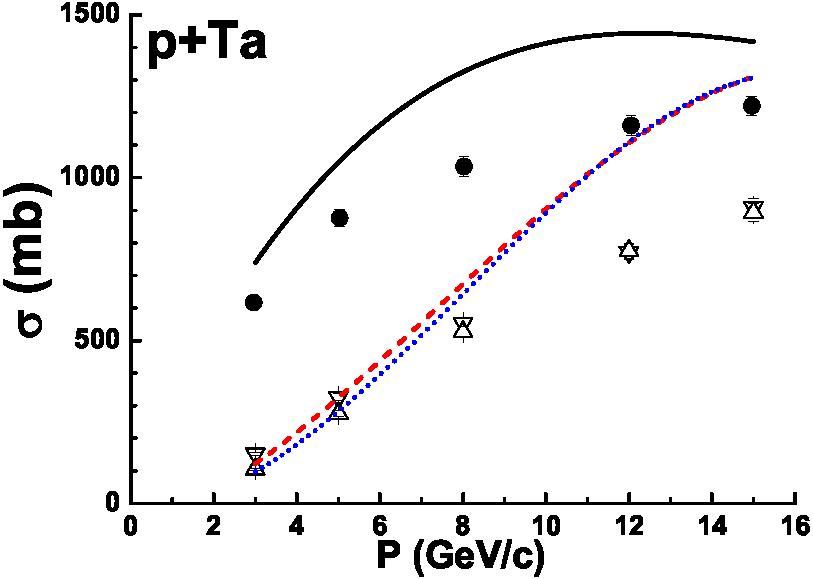
\includegraphics[height=1.8in,width=1.70in]{figures/FTFfig1_1.pdf}
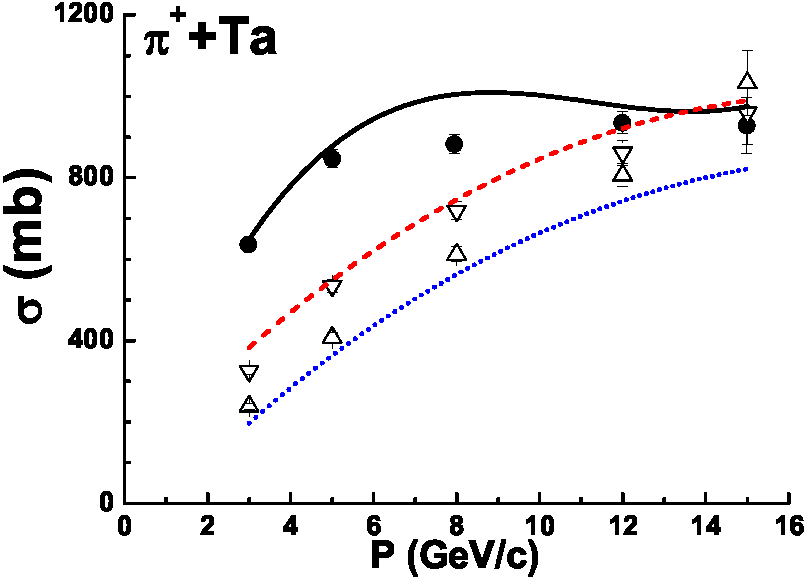
\includegraphics[height=1.8in,width=1.7in]{figures/FTFfig1_2.pdf}
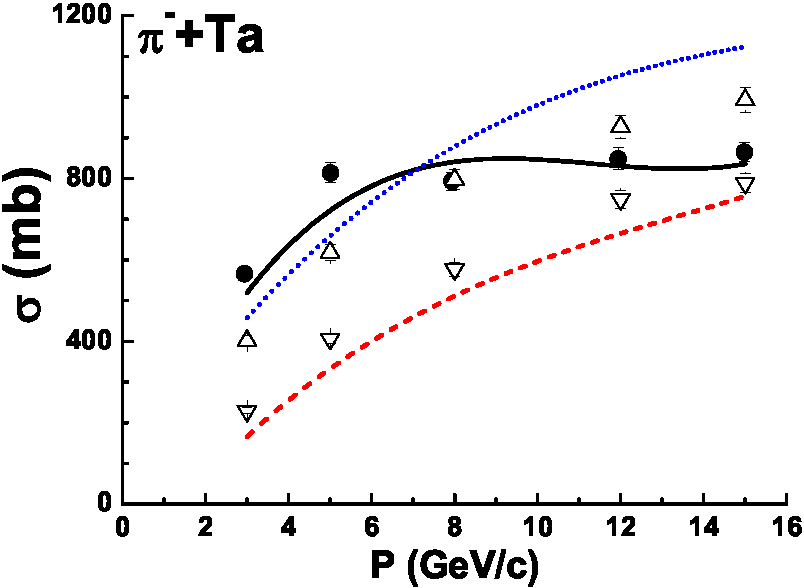
\includegraphics[height=1.8in,width=1.7in]{figures/FTFfig1_3.pdf}
\caption{Inclusive cross sections for $p$, $\pi^+$ and $\pi^-$ production in
         $p{\rm Ta}$, $\pi^+{\rm Ta}$ and $\pi^-{\rm Ta}$ interactions as a 
         function of projectile hadron momentum.  Data from the HARP-CDP 
         group \protect{\cite{hadbib:FTF17}} are shown as closed circles for
         protons and up- and down-triangles for $\pi^+$ and $\pi^-$,
         respectively.  Lines are FTF model calculations: solid for protons,
         dashed and short-dashed for $\pi^+$ and $\pi^-$, respectively.}
\label{had:FTFfig1}
\end{figure}


  \label{had:string}
%%%%%%%%%%%%%%%%%%%%%%%%%%%%%%%%%%%%%%%%%%%%%%%%%%%%%%%%%%%%%%%%%%%%
% cascade.tex
% Authors: Mike Kelsey, Davide Mancusi, Gunter Folger, Dennis Wright
%%%%%%%%%%%%%%%%%%%%%%%%%%%%%%%%%%%%%%%%%%%%%%%%%%%%%%%%%%%%%%%%%%%%
\paragraph{Intranuclear cascade models}
% \noindent {\emph{Intranuclear cascade models}}
Three intranuclear cascade models are now offered in \Gfour{}: Bertini, Binary
and INCL++.  The extended Bertini cascade \cite{hadbib:bert} is valid for
p, n, $\pi$, K, $\Lambda$, $\Sigma$, $\Xi$, $\Omega$ and $\gamma$ projectiles
with incident energies between 0 and 15 GeV.  It is also valid for captured 
$\mu^-$ , $K^-$ and $\Sigma^-$.  Recent extensions allow this model to be used
for cascades initiated by high energy muons and electrons.  Although this model
has its own precompound and deexcitation code, an option exists for using the 
native \Gfour{} precompound and deexcitation modules discussed in the following
section.
%  \cite{hadbib:pnst-preco-2011}.

The Binary cascade \cite{hadbib:binary} simulates p and n-induced cascades
below 10 GeV, and $\pi$-induced cascades below 1.3 GeV.  This is done by 
propagating hadrons in a smooth nuclear potential, and forming and decaying 
strong resonances to produce secondaries.  The model relies on the native 
\Gfour{} precompound and deexcitation code to handle the post-cascade steps. 

The Li\`ege Intranuclear Cascade model (\incl) \cite{hadbib:incl} has seen
extensive development since its introduction in \Gfour{}. The original Fortran 
model was completely redesigned and rewritten in C++ and is now known as 
\inclxx\ \cite{hadbib:inclxx}. It extends the applicability of the legacy 
version up to $\sim15$~GeV incident energy, while remaining physics-wise 
equivalent for nucleon- and pion-induced reactions below 1~GeV. In addition,
\inclxx\ has been extended to handle reactions induced by light ions up to
$A=18$.  By default, \inclxx\ uses the \Gfour{} native de-excitation immediately
after the cascade stage; it does not include an intermediate pre-equilibrium 
step.  Coupling to the \abla\ de-excitation model \cite{hadbib:ablav3} is also
possible.

% Quesada, J.M., Ivantchenko V., Ivantchenko A., Cortes M.A., Folger G.,
% Howard A., Wright D. Recent Developments in Pre-Equilibrium and 
% De-excitation Models in Geant4. Progress in Nuclear Science and Technology. 
% Proceedings of the Joint International Conference Supercomputing in Nuclear 
% Applications and Monte Carlo 2010. October 17-21. Tokyo, Japan.
 \label{had:cascade}
%%%%%%%%%%%%%%%%%%%%%%%%%%%%%%%%%%%%%%%%%%%%%%%%%%%
% precompound.tex
% Author: Jose-Manuel Quesada
%%%%%%%%%%%%%%%%%%%%%%%%%%%%%%%%%%%%%%%%%%%%%%%%%%%
\paragraph{The precompound model}
The native \Gfour{} pre-equilibrium  model is based on a version of the 
semi-classical exciton model \cite{hadbib:gudima83} and is used as the back-end
stage of several cascade and quark-gluon string generators.  It handles the 
de-excitation of the remnant nucleus from its formation immediately following a
cascade or high energy collision, until it reaches equilibrium.  During this 
time, internal transitions of the pre-compound nuclear system compete with 
nucleon and light cluster emissions.  The passage to the state of statistical 
equilibrium, which happens when the transition probabilities for increasing and 
decreasing the exciton number become approximately equal (equilibrium condition),
is roughly characterized by an equilibrium number of excitons $n_{eq}$.  In the
simulation $n_{eq}$ is a calculated number based on the assumption that the 
equilibrium condition is met. 

Some refinements were introduced recently 
\cite{hadbib:calor-2008, hadbib:ijrb-space-2012, hadbib:iaea-spa-2009}, 
namely more realistic inverse cross section parameterizations and combinatorial
factors for particle emission, a phenomenological parameterization of the 
transition matrix elements, and a more physically consistent condition for the 
transition to equilibrium, since in certain circumstances this condition is 
reached well before the previously used rough estimate of $n_{eq}$.

At the end of the pre-equilibrium stage, the residual nucleus should be left in
an equilibrium state, in which the excitation energy is shared by the entire 
nuclear system.  Such an equilibrated compound nucleus is characterized by its 
mass, charge and excitation energy with no further memory of the steps which led
to its formation.

 
%%%%%%%%%%%%%%%%%%%%%%%%%%%%%%%%%%%%%%%%%%%%%%%%%%%%%%%%%%%%%%%%%%%
% deexcitation.tex
% Authors: Vladimir Ivantchenko, Jose Manuel Quesada, Gunter Folger
%%%%%%%%%%%%%%%%%%%%%%%%%%%%%%%%%%%%%%%%%%%%%%%%%%%%%%%%%%%%%%%%%%%
\paragraph{Nuclear de-excitation models}
The final de-excitation of a nucleus to a thermalized state is simulated by
several semi-classical models which are responsible for sampling the 
multiplicity of neutrons, protons, light ions, isotopes, and photons.  They
are:
\begin{itemize}
\item Fermi break-up (FBU) \cite{hadbib:mfm-bondorf-1995},
\item statistical multifragmentation \cite{hadbib:mfm-bondorf-1995},
\item fission, based on the Bohr-Wheeler semi-classical model 
      \cite{hadbib:jinr-fis-1977, hadbib:inr-fis-1993},
\item evaporation of nucleons and light fragments, which is handled by models 
      based on either
\begin{itemize}
  \item the Weisskopf-Ewing model \cite{hadbib:weisskopf-1940} for fragments up
        to and including $\alpha$ particles, or
  \item the generalized evaporation model (GEM) \cite{hadbib:gem-2001} for the 
        emission of fragments with masses up to $^{28}$Mg, and 
\end{itemize}
\item \gclass{G4PhotonEvaporation}, which simulates the emission of  
\begin{itemize}
\item discrete gammas according to the E1, M1 and E2 transition probabilities
      taken from the PhotonEvaporation database, which in turn is based on 
      the Evaluated Nuclear Structure Data File (ENSDF) \cite{hadbib:ENSDF}, 
      and 
\item continuous gammas according to the E1 giant dipole resonance strength 
      distribution.
\end{itemize}
\end{itemize}

These models are managed by the \gclass{G4ExcitationHandler} class, in which
they may be invoked in complement or sometimes concurrently with each other.
Some of them have been thoroughly validated and have undergone continuous 
improvement in recent years \cite{hadbib:calor-2008, hadbib:pmb-fluka-g4-2011}.

In order to properly describe the double differential cross sections and isotope
production data of the IAEA spallation benchmark 
\cite{hadbib-iaea-spa-benchmark,hadbib:iaea-spa-2009}, the standard and GEM 
models were combined to form a hybrid model, and the fission model was improved
\cite{hadbib:pnst-preco-2011,hadbib:ijrb-space-2012,hadbib:iaea-spa-2009}.

For radiobiological applications it is essential that the FBU model be used by 
default for the de-excitation of light fragments (Z $<$ 9, A $<$ 17), taking 
into account Pauli blocking and all possible decay channels into stable and 
long-lived fragments.  Validations
\cite{hadbib:nima-pshenich-2010,hadbib:pmb-fluka-g4-2011}
triggered many of the refinements to this model.

For proton and ion beam therapy applications, the photon evaporation model, 
which is critical for the tracking of the Bragg peak from emitted prompt gammas, 
was improved \cite{hadbib:prompt-gamma-2014}.  The statistical 
multifragmentation model, responsible for the explosive break-up of heavier hot
nuclei  (Z $>$ 8, A $>$ 16, and excitation energy $>$ 3 MeV/u), is relevant 
in simulations of shielding from cosmic radiation and has also been validated
\cite{hadbib:ijrb-space-2012,hadbib:nima-pshenich-2010}. 

 \label{had:deexcitation}

%%%%%%%%%%%%%%%%%%%%%%%%%%%%%%%%%%%%%%%%%%%%%%%%%%%%%%%%%%%%%%%%%
% elastic.tex
% Authors: Vladimir Ivantchenko, Vladimir Grichine, Dennis Wright
%%%%%%%%%%%%%%%%%%%%%%%%%%%%%%%%%%%%%%%%%%%%%%%%%%%%%%%%%%%%%%%%%
\paragraph{Elastic scattering models}
Four options exist in \Gfour{} for the simulation of elastic hadron scattering
from nuclei: the GHEISHA-based and CHIPS-based parameterized models,
the Glauber approach, and diffuse diffraction.

The GHEISHA-based models (\gclass{G4HadronElastic}) \cite{hadbib:gheisha} are
valid for all long-lived hadrons at all incident energies.  They sample the 
momentum transfer from a sum of exponentials whose amplitudes are parameterized
in $Z$, $A$ and incident momentum.  These models are fast, but significantly 
overshoot the data at large angles.

The CHIPS-based models (\gclass{G4ChipsElasticModel}) \cite{hadbib:CHIPS} are
similar, but sample the momentum transfer from a more complex parameterization
which includes details of the nuclear size and potential.  Hence, features like 
diffraction minima are represented.  This model is valid for incident protons,
neutrons, pions, kaons and anti-protons at all energies.

The \gclass{G4ElasticHadrNucleusHE} model depends on Glauber multiple scattering
\cite{hadbib:glauber70} in a nucleus which is described by its impact parameter 
profile.  The energy dependence of the scattering is largely determined by a 
phenomenological combination of hadron-nucleon cross sections.  The model is
valid for all long-lived hadrons of energies greater than 1 GeV.

The \gclass{G4DiffuseElastic} model \cite{hadbib:difel} uses an optical model
of the nucleus and takes into account the diffuse nuclear halo as well as Coulomb 
effects.  It is valid for incident protons, neutrons, pions and kaons of all 
energies.    

The four models are compared to data for 1 GeV protons on silicon in 
Figure~\ref{pSiT1GeVmodsum}.

\begin{figure}
% \centering \includegraphics[height=3.3in,width=3.6in]{figures/pSiT1GeVmodsum.eps}
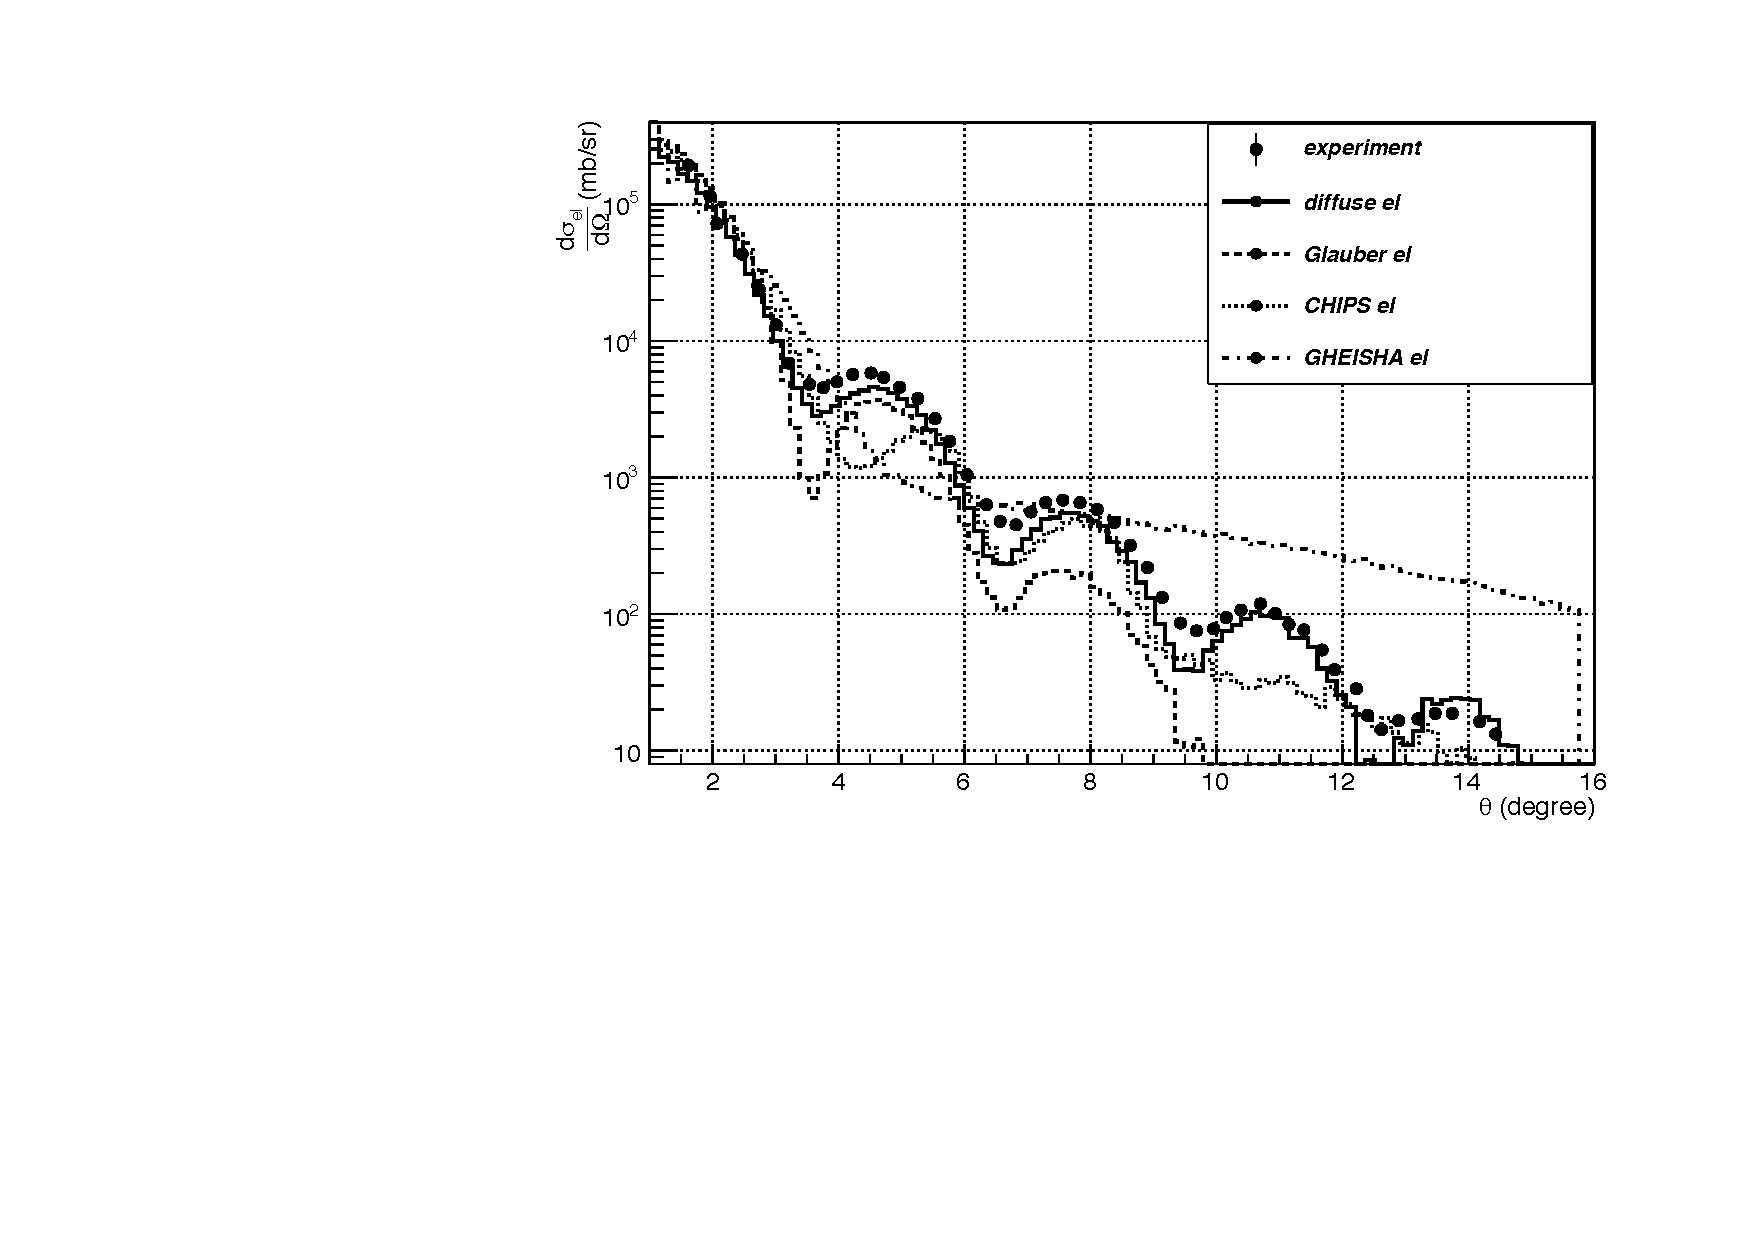
\includegraphics[width=0.5\textwidth]{figures/pSiT1GeVmodsum.pdf}
\caption{Differential elastic scattering cross sections for 1 GeV protons on 
         silicon versus polar scattering angle.  The histograms represent the 
         diffuse, Glauber, CHIPS and GHEISHA models. The solid circles are 
         experimental data~\cite{hadbib:alkh78}.}
\label{pSiT1GeVmodsum}
\end{figure}




%%%%%%%%%%%%%%%%%%%%%%%%%%%%%%%%%%%%%%%%%%%%%%%%%%%
% stopping.tex
% Authors: Julia Yarba, Mike Kelsey, Krzysztof Genser
%%%%%%%%%%%%%%%%%%%%%%%%%%%%%%%%%%%%%%%%%%%%%%%%%%%
\paragraph{Stopping models}
The \Gfour{} toolkit includes processes to simulate the stopping and capture of
hadrons and heavy leptons on nuclei.  Previous parameterized models for $\pi^-$
and $K^-$ capture were replaced by the \Gfour{} Bertini intranuclear cascade for 
negative mesons, baryons and muons, and with the FTF string model for antibaryon
capture and annihilation.  

The Bertini cascade model handles the capture process by selecting a random
location within the nucleus, weighted by the radial nucelon density, to initiate
the cascade process.  The subsequent cascade is propagated using the same code 
used for any other hadron-nucleus interaction.  In the FTF model, the antibaryon
annihilates with a nucleon near the outer ``surface'' of the nucleus, producing 
a small number of pions.  Those secondaries and the excited nucleus are passed 
either to the \Gfour{} de-excitation model (invoked by \gclass{G4PrecompoundModel}),
or to one of the cascade models (Bertini or Binary) for final disposition 
depending on the energy.

Capture of negative muons on nuclei is also handled using the Bertini model.
The muon capture process deals with the atomic capture, the subsequent 
electromagnetic cascade of the muon down to the lowest orbit, including
photon and Auger electron emissions, and the decision about whether the
bound muon should decay in that orbit or be captured into the nucleus.  If
the latter, the Bertini cascade selects a random location within the nucleus 
(weighted as above), where the $\mu^-$ interacts with a proton, producing a 
neutron, neutrino, and one or more radiative photons.  Note that in \Gfour{} 
release 10.0 onward, the radiative cross sections have been set to zero.  As 
above, the neutron is treated as a cascade secondary and processed using the 
existing code of the Bertini model.

 \label{had:stopping}

% needs names of kinematic models 
%%%%%%%%%%%%%%%%%%%%%%%%%%%%%%%%%%%%%%%%%%%%%%%%%%%
% neutrons.tex
% Authors: Tatsumi Koi, Vladimir Ivantchenko
%%%%%%%%%%%%%%%%%%%%%%%%%%%%%%%%%%%%%%%%%%%%%%%%%%%
\paragraph{Low energy neutron models}
As of \Gfour{} 10.0, there were three models treating low energy neutrons with
high precision: NeutronHP, LEND and NeutronXS.  The NeutronHP models, for
elastic, inelastic, capture and fission reactions, have been part of \Gfour{}
for many years \cite{bib:G4}.  They depend on the \Gfour{} Neutron Data Library 
(G4NDL) for cross sections, branching ratios, final state multiplicities and
final state energy and angular distribution parameters.  In its original 
formulation, G4NDL data were drawn from nine different databases,
ENDF/B-VI \cite{hadbib:ENDF}, Brond-2.1 \cite{hadbib:BROND}, CENDL2.2
\cite{hadbib:CENDL}, EFF-3 \cite{hadbib:EFF}, FENDL/E2.0 \cite{hadbib:FENDL},
JEF2.2 \cite{hadbib:JEF}, JENDL-FF \cite{hadbib:JENDLFF}, JENDL-3 
\cite{hadbib:JENDL3} and MENDL-2 \cite{hadbib:MENDL}, 
with the majority coming from the Fusion Evaluated Nuclear Data Library (FENDL).  
This changed in \Gfour{} version 9.5 when G4NDL became solely dependent on US 
ENDF/B-VI and VII (Evalulated Nuclear Data Files) \cite{hadbib:ENDF}. Although 
the other databases are no longer used by G4NDL, they are still available for 
use with \Gfour{}.
  
Many evaluated data libraries, such as ENDF/B-VII.0, JEFF-3.1 and JENDL-4.0, 
have been converted to the \Gfour{} format \cite{hadbib:mendoza} and can be 
obtained at the IAEA Nuclear Data Services website \cite{hadbib:IAEA} .  
% https://www-nds.iaea.org/geant4/.  

NeutronHP was recently extended to include a new, detailed fission fragment 
generator (FFG) which was designed to model the complete detectable portion of
a fission event.  The event is modeled by taking into account mass and momentum 
conservation.  Fission products, from gammas to nuclear fragments are produced 
with realistic energies.  Ternary fission is
supported, even though its probability is low, but is currently limited to 
alpha particles.  The FFG is data-based, but designed to accommodate direct
physics models.  An example of this is symmetric fission and its angular 
dependencies.  This also allows the FFG to fission any isotope, provided that
the daughter product yield data are available. 

Because NeutronHP provides detailed cross sections in the resonance region and 
on-the-fly Doppler broadening, the code can be quite slow and for this reason 
is often not used in physics lists.  In order to provide improved CPU 
performance while retaining part of the NeutronHP precision, the NeutronXS 
elastic and capture cross sections were developed.  These cover neutron energies
from sub-eV up to the TeV range.  Below 20 MeV the detailed cross section data 
of the NeutronHP models are binned logarithmically and tabulated.  This preserves
most of the resonance structure.  At all energies the final state for elastic 
scattering and capture is generated using algorithms from the 
\gclass{G4ChipsElasticModel} and \gclass{G4NeutronRadCapture} models.  The 
NeutronXS cross sections yield a roughly four-fold decrease in CPU time for 
neutron propagation compared to the NeutronHP models and, as of release 10.0,
are now standard in most physics lists.

Another alternative to NeutronHP is the set of LEND (Livermore) neutron models.
These were designed to be faster than NeutronHP, with more streamlined code, but
to provide the same physics.  In the LEND models the cross sections are evaluated 
at a fixed temperature, rather than the on-demand temperature calculations of 
NeutronHP.  This results in a factor five increase in speed.  These models use
the Livermore online database for their reaction data.  It is based in part on 
ENDF/B-VII and can be obtained from the Lawrence Livermore National Laboratory
ftp site \cite{hadbib:llnlftp} .
%  ftp://gdo-nuclear.ucllnl.org/pub .\\



% %%%%%%%%%%%%%%%%%%%%%%%%%%%%%%%%%%%%%%%%%%%%%%%%%%%%%%%%%%%%%%%%%%%%
% cascade.tex
% Authors: Mike Kelsey, Davide Mancusi, Gunter Folger, Dennis Wright
%%%%%%%%%%%%%%%%%%%%%%%%%%%%%%%%%%%%%%%%%%%%%%%%%%%%%%%%%%%%%%%%%%%%
\paragraph{Intranuclear cascade models}
% \noindent {\emph{Intranuclear cascade models}}
Three intranuclear cascade models are now offered in \Gfour{}: Bertini, Binary
and INCL++.  The extended Bertini cascade \cite{hadbib:bert} is valid for
p, n, $\pi$, K, $\Lambda$, $\Sigma$, $\Xi$, $\Omega$ and $\gamma$ projectiles
with incident energies between 0 and 15 GeV.  It is also valid for captured 
$\mu^-$ , $K^-$ and $\Sigma^-$.  Recent extensions allow this model to be used
for cascades initiated by high energy muons and electrons.  Although this model
has its own precompound and deexcitation code, an option exists for using the 
native \Gfour{} precompound and deexcitation modules discussed in the following
section.
%  \cite{hadbib:pnst-preco-2011}.

The Binary cascade \cite{hadbib:binary} simulates p and n-induced cascades
below 10 GeV, and $\pi$-induced cascades below 1.3 GeV.  This is done by 
propagating hadrons in a smooth nuclear potential, and forming and decaying 
strong resonances to produce secondaries.  The model relies on the native 
\Gfour{} precompound and deexcitation code to handle the post-cascade steps. 

The Li\`ege Intranuclear Cascade model (\incl) \cite{hadbib:incl} has seen
extensive development since its introduction in \Gfour{}. The original Fortran 
model was completely redesigned and rewritten in C++ and is now known as 
\inclxx\ \cite{hadbib:inclxx}. It extends the applicability of the legacy 
version up to $\sim15$~GeV incident energy, while remaining physics-wise 
equivalent for nucleon- and pion-induced reactions below 1~GeV. In addition,
\inclxx\ has been extended to handle reactions induced by light ions up to
$A=18$.  By default, \inclxx\ uses the \Gfour{} native de-excitation immediately
after the cascade stage; it does not include an intermediate pre-equilibrium 
step.  Coupling to the \abla\ de-excitation model \cite{hadbib:ablav3} is also
possible.

% Quesada, J.M., Ivantchenko V., Ivantchenko A., Cortes M.A., Folger G.,
% Howard A., Wright D. Recent Developments in Pre-Equilibrium and 
% De-excitation Models in Geant4. Progress in Nuclear Science and Technology. 
% Proceedings of the Joint International Conference Supercomputing in Nuclear 
% Applications and Monte Carlo 2010. October 17-21. Tokyo, Japan.
 \label{had:cascade}

% %%%%%%%%%%%%%%%%%%%%%%%%%%%%%%%%%%%%%%%%%%%%%%%%%%%%%%%%%%
% string.tex
% Authors: Alberto Ribon, Vladimir Uzhinsky, Gunter Folger
%%%%%%%%%%%%%%%%%%%%%%%%%%%%%%%%%%%%%%%%%%%%%%%%%%%%%%%%%%
\paragraph{Quark-gluon string models}
Two models based on quark-parton concepts were implemented in \Gfour{}, the
Quark-Gluon String (QGS) model
% proposed by A. Capella and A.B. Kaidalov
\cite{hadbib:FTF1,hadbib:FTF2} and the Fritiof (FTF) model.
% by Andersson et al.
\cite{hadbib:FTF3,hadbib:FTF4}.
The QGS model is described in \cite{bib:G4}.  A short description of the FTF
model is presented here, but more details are available in the \Gfour{} 
Physics Reference Manual \cite{hadbib:FTF19}.

%of the FTF model will be presented which is
%in production PhysicsLists of \Gfour used by LHC experiments.

The FTF model is used in \Gfour{} to simulate the following interactions:
hadron-nucleus at incident laboratory hadron momenta $>$ 3--5 GeV/c, 
nucleus-nucleus at incident laboratory hadron momenta $>$ 2--3 GeV/c/nucleon,
antibaryon-nucleus at all energies, and antinucleus-nucleus.
Because the model does not include multi-jet production in hadron-nucleon 
interactions, the upper limit of its validity range is estimated to be 1~TeV/c 
per hadron.

The modeling of hadron-nucleon interactions in the FTF model includes the
simulation of elastic scattering, binary reactions such as 
$NN\rightarrow N\Delta$ and $\pi N\rightarrow \pi \Delta$, single diffractive 
and non-diffractive events, and annihilation in anti-baryon-nucleon interactions.
Interactions proceed by the production of one or two unstable objects called 
quark-gluon strings.  If only one string is created, the process is called 
diffraction dissociation.  

In the \Gfour{} implementation single diffraction dissociation is simulated 
separately from non-diffractive interactions.  A special function which 
corresponds to a weighted simulation of the diffraction dissociation was
introduced to perform this separation.  In most other Fritiof-based models 
this separation is governed by a single parameter, which is not sufficient for
a correct description of the large set of experimental data. 

Once formed, strings may interact with other nucleons in hadron-nucleus and 
nucleus-nucleus collisions, producing additional strings.  Strings with 
sufficiently large mass ($>$ 1.2~GeV) may in general have kinks, which are
treated as emitted gluons which decay into quark-antiquark pairs.  This feature
is required in order to reproduce particle multiplicities observed in hadronic 
interactions at high energies.  However, the current FTF implmentation does not 
handle kinks, hence the TeV/c upper limit.  

% Because multi-gluon production in elementary interactions is
% not included in FTF, the upper limit of the model's validity is estimated to be 
% 1~TeV, sufficient for most applications of \Gfour{}.

Hadron-nucleon scattering within the model uses the elastic and inelastic cross 
sections taken from the CHIPS parameterizations \cite{hadbib:CHIPS}. 
Cross sections for binary reactions and diffraction dissociation were implemented
directly in the FTF model as parameterizations of data.  Here the cross sections
for the unstable objects were taken to be the same as those for stable objects
with the same quark content.  

Once the unstable objects are produced, the LUND string fragmentation model is 
used to decay them \cite{hadbib:FTF7}.  The parameters of this model were tuned
to experimental data and the available phase space was restricted to take into 
account low mass string fragmentation.  The formation time of hadrons was also 
applied.

To simulate hadron-nucleus and nucleus-nucleus scattering it is necessary to 
embed the hadron-nucleon interaction in the nuclear environment.  This was done
by first assuming a Woods-Saxon parameterization of the one-particle nuclear 
density for medium and heavy nuclei and a harmonic oscillator shape for light 
nuclei.  Center-of-mass correlations and short-range nucleon-nucleon 
correlations were taken into account.  A simplified Glauber model was used to 
sample the multiplicity of intra-nuclear collisions.  Screening was not 
considered; estimates and data indicate that it decreases the total 
hadron-nucleus cross sections by 3--5\%, while the inelastic hadron-nucleus 
cross sections are practically unchanged \cite{hadbib:Alvi}.  Hence any effect 
on the multiplicity of produced particles is expected to be small.

The number of string objects in non-diffractive interactions is proportional to
the number of participating nucleons. Thus, multiplicities in hadron-nucleus and
nucleus-nucleus interactions are larger than those in elementary interactions.
It is assumed that the reaction creating unstable strings in hadron-nucleus
collisions is analogous to that in nucleus-nucleus collisions.

It is known that the Glauber approximation used in this and other string models
does not provide enough intra-nuclear collisions for a correct description of
nuclear destruction.  Traditional cascade models would fulfill this need, except 
that they produce too many particles.  Reggeon theory has been proposed to solve
this problem \cite{hadbib:FTF18}, but the detailed calculation required was not
appropriate for a reasonably fast computer code.  A simplified implementation in
\Gfour{} assumes \cite{hadbib:FTF10} that participating nucleons predicted by the 
Glauber approximation initiate low energy reggeon exchanges in the spectator 
part of a target nucleus.  This reggeon theory inspired model (RTIM) provides 
the right number of fast nucleons ejected during nuclear destruction and 
describes secondary particle intra-nuclear cascading \cite{hadbib:FTF8}.   

The collective nature of nuclear destruction led to the introduction of a new
"Fermi motion" \cite{hadbib:FTF9,hadbib:FTF10} simulation which is a refined 
algorithm for putting involved nucleons on the mass-shell.  As shown in 
Figure~\ref{had:FTFfig1}, this provides sufficient agreement with experimental
data in the transition region, around 3~GeV/c.

When the cascading is finished, the excitation energies of residual nuclei are
estimated in the ``wounded nucleon'' approximation \cite{hadbib:FTF11}. This 
allows for a direct coupling of the FTF model to the \Gfour{} precompound model
and its nuclear fragmentation sub-models.  The determination of the particle
formation time also allows coupling of the FTF model to the \Gfour{} Binary 
cascade model \cite{hadbib:FTF12}.

%The Ultra-Relativistic Quantum Molecular Dynamic model (UrQMD) \cite{hadbib:FTF13}
%simulates the binary reactions, but it seems to as that their cross sections are
%not tuned quite well. 

% An effort is underway to fit the cross sections in the FTF model, but up to
% now only low mass resonances have been considered. It is thus expected that the
% FTF model is not entirely correct at projectile energies below 3--5 GeV.

% A peculiarity of the \Gfour Fritiof model implementation is the separate 
% simulation of the single diffraction dissociation and non-diffractive 
% interactions. In most Fritiof-based models the separation between the processes
% is governed by a single parameter.  This, however, is not sufficient for a 
% correct description of the large set of experimental data.  A special function
% for this separation was therefore introduced, which corresponds to a weighted 
% simulation of the diffraction dissociation.

Two additional innovations were made in the FTF model, one dealing with low-mass
strings and the other making multiplicity corrections in hadron-nucleus and
nucleus-nucleus reactions.
   
All Monte Carlo event generators are challenged with the correct treatment 
of low mass strings. Such a string is typically handled by first checking that
it can decay into two low mass particles. If it can, the decay is simulated;
otherwise, the string is converted into a hadron.  This step violates 
energy-momentum conservation and the momenta of all other produced particles
must be adjusted to correct for this.  In the FTF model all strings with 
sufficiently large mass are allowed to decay to two particles.  As a result, the
cross sections of the reactions $\bar p+p \rightarrow \bar n+n$, 
$\bar p+p \rightarrow \bar \Lambda+\Lambda$, and so on, are reproduced. In the 
case of a two-particle decay, all possible final states are considered, and one 
is chosen according to its phase space volume. For other final states, standard 
string fragmentation or direct production of a hadron is possible.  

% Strings with sufficiently large mass ($>$ 1.2 GeV) can have a kink. The kink is
% treated as a gluon which decays into a quark-antiquark pair. This is needed
% to reproduce particle multiplicities observed in hadronic interactions. The 
% UrQMD model \cite{hadbib:FTF13}, for example, does not consider kinky strings,
% while the Hijing model \cite{hadbib:FTF14} assumes copious gluon production in 
% hard and semi-hard interactions. The Fritiof 7.0 model \cite{hadbib:FTF15} also
% considers gluon production. Because multi-gluon production in elementary 
% interactions is not included in the \Gfour FTF model, its upper limit of 
% application is estimated to be 1 TeV, sufficient for most applications of \Gfour.

Multiplicity corrections in hadron-nucleus and nucleus-nucleus interactions are 
necessary when computing the number $N_{bin}$ of intra-nuclear collisions.  The
distribution of $N_{bin}$ is usually obtained by applying the asymptotic AGK 
cutting rules \cite{hadbib:FTF16} to the Glauber amplitude for elastic 
scattering.  These rules must be corrected for finite energies. Because there is
no defined prescription for making these corrections, a phenomenological 
approach, taking into account formation time and using HARP-CDP data 
\cite{hadbib:FTF17}, was adopted.

%{\bf suggest to remove all this and quote an article with details:\\
%As known, a simple cascade model considers only pions and nucleons. Due to this
%it cannot work when resonance production is a dominating process in hadronic
%interactions. But if the energy is sufficiently low the resonances can decay
%before a next possible collision, and the model can be valid.
%  OK above ??
% Let $p$ be the momentum
%of a produced resonance ($\Delta$). The average life time of the resonance in
%its rest frame is $1/\Gamma$. In the laboratory frame the time is
%$E_\Delta/\Gamma m_\Delta$. During this time, the resonance will fly a distance
%$\bar{l}=v\ E_\Delta/\Gamma m_\Delta=p/\Gamma m_\Delta$. If the distance is less
%than an average distance between nucleons in nuclei ($\bar{d}\sim 2$ fm),
%the model can be applied. From the condition, we have:
%$
%p\leq \bar{d}\ \Gamma m_\Delta \sim 1.5
%$
%(GeV/c).
%
%Direct $\Delta$-resonance production takes place in $\pi N$ interactions at low energies.
%Thus the model cannot work well at a momentum of pions above 2 GeV/c. In nucleon-nucleon
%interactions, due to momentum transfer to a target nucleon, the boundary can be higher.
%
%Returning back to the FTF model, let us assume that projectile originated strings
%have an average life time $1/\Gamma$, and an average mass $m^*$. The strings can
%interact on average with $\bar{l}/\bar{d}=p/\Gamma m^*\bar{d}=p/p_0$ nucleons.
%Here $p_0$ is a new parameter. According to our estimates it is about 2 -- 3 GeV/c.
%Thus, we can assume that at any energy there is a maximum number of intra-nuclear
%collisions in the FTF model -- $\nu_{max}=p/p_0$.
%This restriction is implemented in the current version of the FTF model, and puts
%a low boundary of the model application region to 3--5 GeV/c. For the determination
%of the $p_0$ parameter we used the HARP-CDP data \cite{hadbib:FTF17}.
%
%As known, the Glauber approximation used in the Fritiof model and in the other
%string models does not provide enough intra-nuclear collisions for a correct
%description of a nuclear destruction. Additional cascading in nuclei is needed!
%Usage of a standard cascade for secondary particle interactions leads to a large
%multiplicity of produced particles. Usually, it is assumed that an inclusion of
%a secondary particle's formation time can help to solve this problem, but there
%is no unified solution. The concept of the formation time was criticized in
%the paper \cite{hadbib:FTF18} where the intra-nuclear cascade was considered
%from the reggeon theory point of view. Because we were not be able to implement
%a complicated reggeon calculation scheme, we have assumed \cite{hadbib:FTF10}
%that participating nucleons predicted by the Glauber approximation initiate
%low energy reggeon exchanges in a spectator part of a target nucleus (reggeon
%cascading). This provide us with an enough amount of fast nucleons ejected at
%a target nucleus destruction.
%
% This collective nature of the destruction
%pushed us to introduce a new "Fermi motion" simulation which is a refined
%algorithm of putting of involved nucleons onto mass-shell.  All of these
%allowed us to obtain a smooth transition from the FTF model and low energy
%Bertini and Binary cascade models of \Gfour (see Fig.~\ref{had:FTFfig1}a).
%
%The main problem now is an accounting of the diffraction dissociation in
%hadron-nucleus and nucleus-nucleus interactions. A transition of a projectile
%particles into a diffractive system and back during elastic scattering on a nucleus
%has to be suppressed by the nuclear form-factor. Due to this a projectile
%diffraction dissociation in inelastic interactions has to be also suppressed
%according to the reggeon phenomenology. One cannot apply this consideration
%to a target nucleon diffraction, and one can assume that they can dissociate.
%But the calculations presented in Fig.~\ref{had:FTFfig1} were done without
%the suppression for $p{\rm Ta}$ interactions, and with full suppression for
%$\pi {\rm Ta}$ interactions. Another choice makes the description worse.
%The question is now under the study.
%}

\begin{figure}
\centering
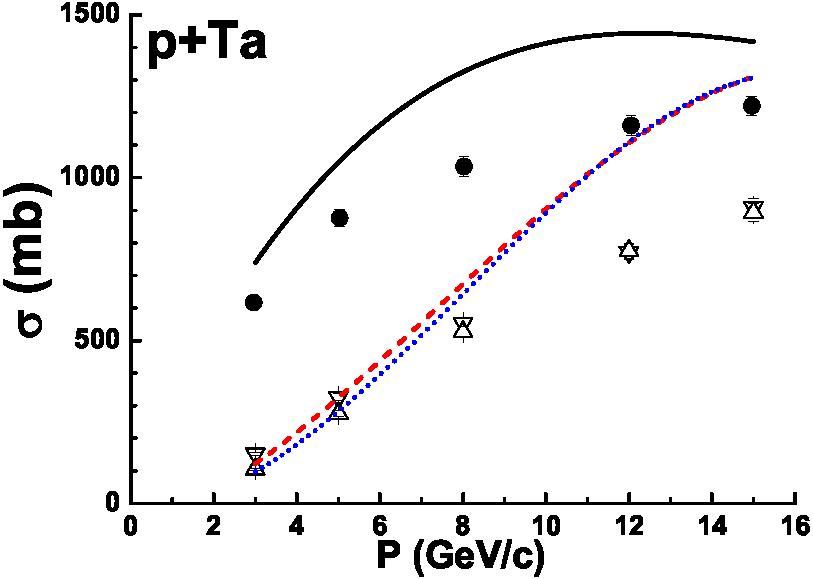
\includegraphics[height=1.8in,width=1.70in]{figures/FTFfig1_1.pdf}
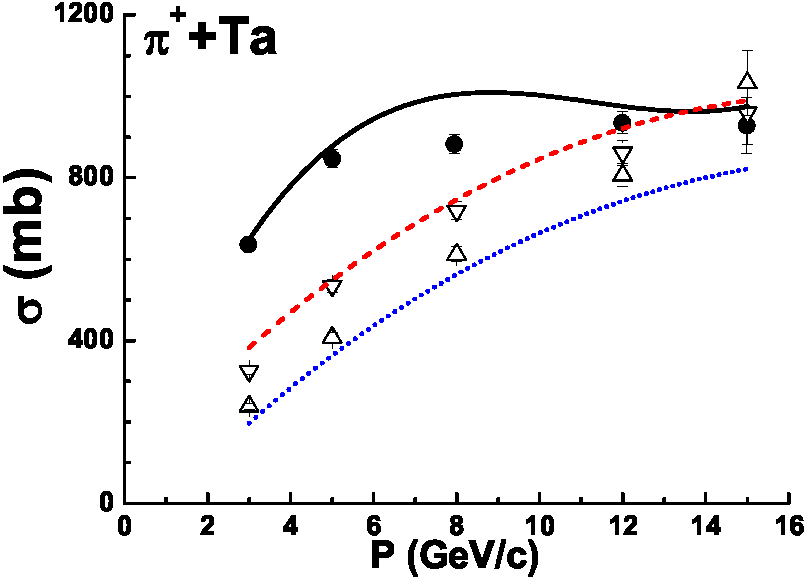
\includegraphics[height=1.8in,width=1.7in]{figures/FTFfig1_2.pdf}
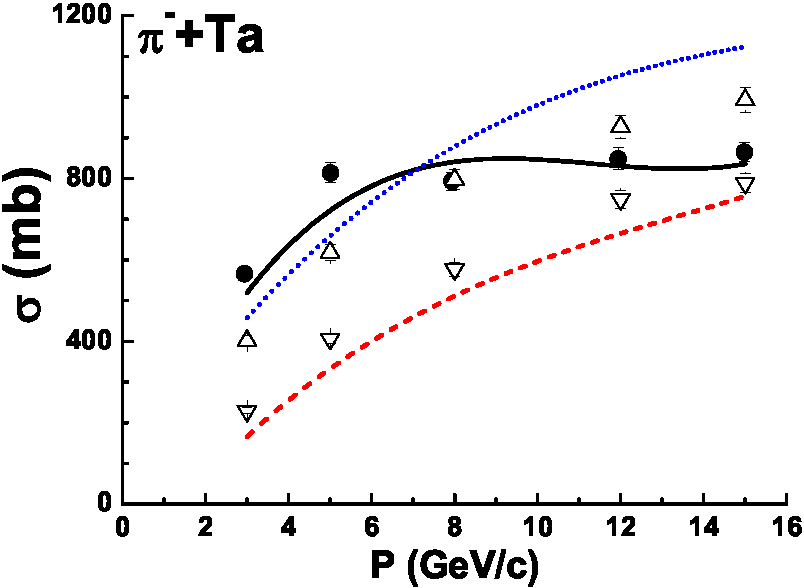
\includegraphics[height=1.8in,width=1.7in]{figures/FTFfig1_3.pdf}
\caption{Inclusive cross sections for $p$, $\pi^+$ and $\pi^-$ production in
         $p{\rm Ta}$, $\pi^+{\rm Ta}$ and $\pi^-{\rm Ta}$ interactions as a 
         function of projectile hadron momentum.  Data from the HARP-CDP 
         group \protect{\cite{hadbib:FTF17}} are shown as closed circles for
         protons and up- and down-triangles for $\pi^+$ and $\pi^-$,
         respectively.  Lines are FTF model calculations: solid for protons,
         dashed and short-dashed for $\pi^+$ and $\pi^-$, respectively.}
\label{had:FTFfig1}
\end{figure}


  \label{had:string}


%\subsubsection{Nuclear de-excitation model}
% \label{sec:evaporation}

% %%%%%%%%%%%%%%%%%%%%%%%%%%%%%%%%%%%%%%%%%%%%%%%%%%%
% precompound.tex
% Author: Jose-Manuel Quesada
%%%%%%%%%%%%%%%%%%%%%%%%%%%%%%%%%%%%%%%%%%%%%%%%%%%
\paragraph{The precompound model}
The native \Gfour{} pre-equilibrium  model is based on a version of the 
semi-classical exciton model \cite{hadbib:gudima83} and is used as the back-end
stage of several cascade and quark-gluon string generators.  It handles the 
de-excitation of the remnant nucleus from its formation immediately following a
cascade or high energy collision, until it reaches equilibrium.  During this 
time, internal transitions of the pre-compound nuclear system compete with 
nucleon and light cluster emissions.  The passage to the state of statistical 
equilibrium, which happens when the transition probabilities for increasing and 
decreasing the exciton number become approximately equal (equilibrium condition),
is roughly characterized by an equilibrium number of excitons $n_{eq}$.  In the
simulation $n_{eq}$ is a calculated number based on the assumption that the 
equilibrium condition is met. 

Some refinements were introduced recently 
\cite{hadbib:calor-2008, hadbib:ijrb-space-2012, hadbib:iaea-spa-2009}, 
namely more realistic inverse cross section parameterizations and combinatorial
factors for particle emission, a phenomenological parameterization of the 
transition matrix elements, and a more physically consistent condition for the 
transition to equilibrium, since in certain circumstances this condition is 
reached well before the previously used rough estimate of $n_{eq}$.

At the end of the pre-equilibrium stage, the residual nucleus should be left in
an equilibrium state, in which the excitation energy is shared by the entire 
nuclear system.  Such an equilibrated compound nucleus is characterized by its 
mass, charge and excitation energy with no further memory of the steps which led
to its formation.



% %%%%%%%%%%%%%%%%%%%%%%%%%%%%%%%%%%%%%%%%%%%%%%%%%%%%%%%%%%%%%%%%%%%
% deexcitation.tex
% Authors: Vladimir Ivantchenko, Jose Manuel Quesada, Gunter Folger
%%%%%%%%%%%%%%%%%%%%%%%%%%%%%%%%%%%%%%%%%%%%%%%%%%%%%%%%%%%%%%%%%%%
\paragraph{Nuclear de-excitation models}
The final de-excitation of a nucleus to a thermalized state is simulated by
several semi-classical models which are responsible for sampling the 
multiplicity of neutrons, protons, light ions, isotopes, and photons.  They
are:
\begin{itemize}
\item Fermi break-up (FBU) \cite{hadbib:mfm-bondorf-1995},
\item statistical multifragmentation \cite{hadbib:mfm-bondorf-1995},
\item fission, based on the Bohr-Wheeler semi-classical model 
      \cite{hadbib:jinr-fis-1977, hadbib:inr-fis-1993},
\item evaporation of nucleons and light fragments, which is handled by models 
      based on either
\begin{itemize}
  \item the Weisskopf-Ewing model \cite{hadbib:weisskopf-1940} for fragments up
        to and including $\alpha$ particles, or
  \item the generalized evaporation model (GEM) \cite{hadbib:gem-2001} for the 
        emission of fragments with masses up to $^{28}$Mg, and 
\end{itemize}
\item \gclass{G4PhotonEvaporation}, which simulates the emission of  
\begin{itemize}
\item discrete gammas according to the E1, M1 and E2 transition probabilities
      taken from the PhotonEvaporation database, which in turn is based on 
      the Evaluated Nuclear Structure Data File (ENSDF) \cite{hadbib:ENSDF}, 
      and 
\item continuous gammas according to the E1 giant dipole resonance strength 
      distribution.
\end{itemize}
\end{itemize}

These models are managed by the \gclass{G4ExcitationHandler} class, in which
they may be invoked in complement or sometimes concurrently with each other.
Some of them have been thoroughly validated and have undergone continuous 
improvement in recent years \cite{hadbib:calor-2008, hadbib:pmb-fluka-g4-2011}.

In order to properly describe the double differential cross sections and isotope
production data of the IAEA spallation benchmark 
\cite{hadbib-iaea-spa-benchmark,hadbib:iaea-spa-2009}, the standard and GEM 
models were combined to form a hybrid model, and the fission model was improved
\cite{hadbib:pnst-preco-2011,hadbib:ijrb-space-2012,hadbib:iaea-spa-2009}.

For radiobiological applications it is essential that the FBU model be used by 
default for the de-excitation of light fragments (Z $<$ 9, A $<$ 17), taking 
into account Pauli blocking and all possible decay channels into stable and 
long-lived fragments.  Validations
\cite{hadbib:nima-pshenich-2010,hadbib:pmb-fluka-g4-2011}
triggered many of the refinements to this model.

For proton and ion beam therapy applications, the photon evaporation model, 
which is critical for the tracking of the Bragg peak from emitted prompt gammas, 
was improved \cite{hadbib:prompt-gamma-2014}.  The statistical 
multifragmentation model, responsible for the explosive break-up of heavier hot
nuclei  (Z $>$ 8, A $>$ 16, and excitation energy $>$ 3 MeV/u), is relevant 
in simulations of shielding from cosmic radiation and has also been validated
\cite{hadbib:ijrb-space-2012,hadbib:nima-pshenich-2010}. 

 \label{had:deexcitation}

% needs discussion of G4NuclNuclDiffuseElastic
%%%%%%%%%%%%%%%%%%%%%%%%%%%%%%%%%%%%%%%%%%%%%%%%%%%%%
% nucleusnucleus.tex
% Authors: Davide Mancusi, Dennis Wright
%%%%%%%%%%%%%%%%%%%%%%%%%%%%%%%%%%%%%%%%%%%%%%%%%%%%%
\paragraph{Nucleus-nucleus models}
As of release 10.0 there were six \Gfour{} models capable of handling
nucleus-nucleus collisions: binary light ion, abrasion/ablation, 
electromagnetic dissociation, QMD, INCL++ and FTF models.

The Binary Light Ion model handles collisions in which either the projectile or
the target has mass $A < 13$.  Based on the \Gfour{} Binary Cascade model 
\cite{hadbib:binary}, it is valid above 80 MeV and below 10 GeV/nucleon. 

Operating over a similar energy range, but without limits on the projectile or
target masses, the \gclass{G4WilsonAbrasion} model, based on NUCFRG2 
\cite{hadbib:wilson} is faster, but less detailed, than the Binary Light Ion 
model.  It is a geometrical model in which a portion of the target nucleus along
the incident path of the projectile is gouged out, forming a forward-going 
compound nucleus and a residual target.  The associated Wilson ablation model is
used to de-excite the products of the initial collision.

Also based on NUCFRG2, \gclass{G4EMDissociation} is an electromagnetic 
dissociation model provided to handle the production of nuclear fragments 
resulting from the exchange of virtual photons between projectile and target 
nuclei.  This model is valid for nuclei of all masses and all energies.
  
QMD (Quantum Molecular Dynamics) is a native \Gfour{} model based on an extension
of the classical molecular dynamics model introduced in release 9.1.  Each 
nucleon in the target and projectile nuclei is treated as a gaussian wave packet
which propagates with scattering through the nuclear medium, taking Pauli 
exclusion into account.  The nuclear potential is that of two merging nuclei and
its shape is re-calculated at each time step of the collision.  
Participant-participant scattering is also taken into account.  
These last two facts combine to make the model rather slow for collisions of
heavy nuclei, but the production of nuclear fragments versus energy is well 
reproduced.  The model is valid for all projectile-target combinations and for
projectile energies between 100 MeV/nucleon and 10 GeV/nucleon.  Since its
introduction, the model was made Lorentz covariant and improvements were made in
fragment prodcution at relativistic energies.
 
The \inclxx\ model, covered above, can also accommodate nucleus-nucleus 
reactions provided the projectile has a mass below $A = 19$ and an energy 
between 1 MeV/nucleon and 3 GeV/nucleon.  A broad validation campaign on 
heterogeneous observables has shown that, in spite of the conceptual 
difficulties, the extended \inclxx\ model yields predictions in fair agreement 
with experimental data; it is however crucial to make a suitable choice for the 
coupling with the statistical de-excitation model.

The FTF model, covered above, is capable of modeling 
reactions with all combinations of projectile and target mass, with projectile 
energies in the range 2 GeV/nucleon to about 1 TeV/nucleon.  However, validation
of this application is still in progress, and collisions of two heavy nuclei are 
expected to be computationally expensive.



%%%%%%%%%%%%%%%%%%%%%%%%%%%%%%%%%%%%%%%%%%%%%%%%%%%
% radioactivedecay.tex
% Author: Dennis Wright
%%%%%%%%%%%%%%%%%%%%%%%%%%%%%%%%%%%%%%%%%%%%%%%%%%%
\paragraph{The radioactive decay process}
The \gclass{G4RadioactiveDecay} process and model handles $\alpha$, $\beta^-$,
$\beta^+$, isomeric transition (IT) and electron capture (EC) decays, and can be
applied to generic ions both in flight and at rest.   

Details for each decay or level transition, such as nuclear level energies, 
branching ratios and reaction Q values, come from the \Gfour{} RadioactiveDecay 
database, which currently contains entries for 2798 nuclides.  Details of 
specific gamma levels used for IT decays are taken from the \Gfour{} 
PhotonEvaporation database.  Both the PhotonEvaporation and RadioactiveDecay 
databases take their data from the Evaluated Nuclear Structure Data File (ENSDF)
\cite{hadbib:ENSDF} and have recently been rationalized so that their common 
nuclear levels have identical values.

Beginning with \Gfour{} release 9.6 and continuing through releases currently in
preparation, a number of improvments have been made to the radioactive decay 
package.  These include:

\begin{itemize}
\item a complete review of the PhotonEvaporation and RadioactiveDecay databases,
      and updating to the 2013 version of ENSDF,
\item the ability to model decays with lifetimes as short as 1 ps,
\item decays of observationally stable ground states, that is, those having
      very long predicted life times, but which have not yet been observed to 
      decay,  
\item the addition of unique first, second and third forbidden $\beta^-$ and
      $\beta^+$ decays,
\item the default invocation of the atomic relaxation model after IT and EC 
      decays, and 
\item improved energy conservation for all decay modes.
\end{itemize}



%%%%%%%%%%%%%%%%%%%%%%%%%%%%%%%%%%%%%%%%%%%%%%%%%%%
% gamleptnuclear.tex
% Authors: Dennis Wright, Mike Kelsey
%%%%%%%%%%%%%%%%%%%%%%%%%%%%%%%%%%%%%%%%%%%%%%%%%%%
\paragraph{Gamma- and lepto-nuclear models}
Due to the relatively small electromagnetic coupling, gamma- and lepto-nuclear
reactions play a small role in high energy physics calorimetry. They are 
important, though, for nuclear, medium energy and cosmic ray physics.  For this 
reason \Gfour{} models for these reactions were extended and improved.  

The \gclass{G4PhotoNuclearProcess} is implemented by two models, the Bertini 
cascade below 3.5 GeV and the Quark-Gluon-String (QGS) model above 3 GeV.  Both
models treat the incident gamma as if it were a hadron interacting with a 
nucleon within the nuclear medium.  Nevertheless, below 30 MeV the Bertini model
does capture some collective nuclear effects such as the giant dipole resonance.

Both the electro-nuclear and muon-nuclear models
(\gclass{G4ElectroVD\allowbreak{}Nuclear\allowbreak{}Model}
and \gclass{G4MuonVD\allowbreak{}Nuclear\allowbreak{}Model}) exploit two
features of the hybrid electromagnetic hadronic interaction: the factorization
of the interaction into separate hadronic and electromagnetic parts and the 
treatment of the exchanged 
photon as if it were a hadron.  The electromagnetic vertex produces a virtual 
photon from a two-dimensional cross section table and uses the method of 
equivalent photons to make the photon real.  As in the photo-nuclear case 
mentioned above, the photon is then treated as a hadron for the remainder of the
interaction.  For real photons below 10 GeV the Bertini cascade handles the 
interaction;  above 10 GeV the photon is converted to a neutral pion and the 
interaction proceeeds using the FTF string model.

 \label{had:gamleptnucleus}

%%%%%%%%%%%%%%%%%%%%%%%%%%%%%%%%%%%%%%%%%%%%%%%%%%%
% obsoletemodels.tex
% Author: Dennis Wright
%%%%%%%%%%%%%%%%%%%%%%%%%%%%%%%%%%%%%%%%%%%%%%%%%%%
\paragraph{Obsolete models}
The first \Gfour{} hadronic models, the Low Energy Parameterized (LEP) and 
High Energy Parameterized (HEP), were both re-engineered versions of the Fortran
code Gheisha \cite{hadbib:gheisha}.  In their original form they were designed
and tuned to reproduce high energy shower shapes.  They conserved energy on
average, but not on an event-by-event basis.  With the advent of more 
theoretically detailed models, both LEP and HEP models were removed from version
10.0 of the toolkit.

Prior to \Gfour{} 10.0, a number of models and cross section sets dealing
with nuclear de-excitation, hadron capture, gamma-nuclear and lepton-nuclear 
reactions were implemented by the Chiral Invariant Phase Space (CHIPS) package.
Since version 10.0, most of these reactions have been implemented by other models 
although some of the cross sections still maintain the original CHIPS coding.

Lastly, the isotope production model, used to count recoil nuclei produced in
various reactions, was removed in version 10.0, as all hadronic models now 
produce recoil nuclei explicitly.





  % Authors: Gunter Folger
  %%%%%%%%%%%%%%%%%%%%%%%%%%%%%%%%%%%%%%%%%%%%%%%%%%%
% physicslists.tex
%%%%%%%%%%%%%%%%%%%%%%%%%%%%%%%%%%%%%%%%%%%%%%%%%%%
\label{sec:physlists}
\subsection{\textbf{Physics Lists}}
In \Gfour{}, physics lists refer to classes which provide the means to collect
and organize the particle types, physics models and cross sections required for
a particular simulation application.  These classes allow physics processes to 
be registered to the run manager which in turn attaches them to tracks so that 
they may interact properly with the simulation geometry.

When originally conceived, physics lists were intended to give the user maximum 
flexibility and responsibility to choose and combine particles, models and cross
sections.  Developers thus did not provide default physics or specific physics 
combinations to users, except in certain custom situations.  It eventually 
became clear from user requests that ready-made and validated physics modules 
were desired which could be easily plugged into user physics lists.  This led to
the development of several ``reference'' physics lists which were specialized to
provide standard behavior in various application domains.  In medical or space 
applications, for example, detailed atomic physics may be required, while for 
high energy physics it is not.  In high energy applications TeV scale physics is
important, but not for medim and low energies.   

While the basic, maximally flexible physics list classes are still available
and fully documented in the \Gfour{} Application Developers Guide
\cite{bib:AppDevGuide}, the focus here is on prepared, modular physics lists 
which are organized around builders and constructors.  

\subsubsection{Constructors} \label{subsec:ctors}
All prepared physics lists in \Gfour{} derive from the class
\gclass{G4VModular\allowbreak{}PhysicsList} which in turn derives from the base
class \gclass{G4VUserPhysicsList}.  \gclass{G4VModular\allowbreak{}PhysicsList}
maintains a vector of physics modules, each of which is an implementation of the 
\gclass{G4VPhysics\allowbreak{}Constructor} class.  A module, referred to here 
as a physics constructor, enables the logical grouping of related physics 
models, cross 
sections and particles.  This allows the most accurate and CPU-appropriate 
physics models to be applied to given energy ranges and particle types.  The 
\gmethod{ConstructParticle()} and \gmethod{ConstructProcess()} methods of 
\gclass{G4VPhysics\allowbreak{}Constructor} can be used to instantiate the 
particle types needed for a given application, and to assign models and cross
sections to 
processes.  For example, all pions and kaons could be instantiated in a meson 
physics constructor, which would also assign two hadronic models, a cascade 
model at low energies and parton string model at high energies, to the 
processes pertaining to pions and kaons.

The chosen electromagnetic and hadronic constructors are stored in a vector, 
which makes it easy to build a new physics list by adding, removing or replacing
physics constructors.  A large collection of these constructors is included in 
the \Gfour{} toolkit.  The electromagnetic constructors are listed in 
Table~\ref{em:physl} and examples for using them \cite{bib:uni} are distributed
with the release. 

\begin{table*}
\caption{List of default and optional \Gfour{} EM physics constructor classes.
         One of several optional EM physics constructors may be chosen by 
         appending its shorthand name, listed in the ``Extension'' column, to 
         the name of a basic physics list, such as FTFP\_BERT\_ENV, for example.
         WVI refers to the Wenzel multiple scattering model as implemented by 
         V. Ivantchenko.}
\label{em:physl}
\begin{center}
\begin{tabular}{llll}
\hline
Physics Constructor Name& Application& Extension & Comment \\ \hline
\gclass{G4EmStandardPhysics} & HEP &  &default (ATLAS)\\
\gclass{G4EmStandardPhysics\_option1} & & EMV & simplified (CMS)\\
\gclass{G4EmStandardPhysics\_option2} & & EMX & simplified (LHCb)\\
\hline
\gclass{G4EmStandardPhysics\_option3} & space \& & EMY & detailed  \\
                             &  medicine &     & standard models\\
\gclass{G4EmLivermorePhysics} & & LIV & detailed  \\
                     &       &          &  Livermore models\\
\gclass{G4EmPenelopePhysics} &  & PEN & detailed \\ 
                    &  &     & Penelope models\\
\gclass{G4EmStandardPhysics\_option4} &  & EMZ & combining \\
                             &  &     & best models\\
\hline
\gclass{G4EmLivermorePolarizedPhysics} &  &  & polarized models\\
\gclass{G4EmLowEPPhysics} &  &  & new low energy models\\
\gclass{G4EmStandardPhysicsWVI} &  &  & WVI multiple scattering\\
\gclass{G4EmStandardPhysicsSS} &  &  & single scattering \\
\hline
\gclass{G4EmDNAPhysics} & DNA &  & default for DNA physics \\
\gclass{G4EmDNAPhysics\_option1} & DNA &  & WVI multiple scattering \\
\hline
\gclass{G4OpticalPhysics} & all &  & production and transport \\
                 &     &  & of optical photons \\
\hline
\end{tabular}
\end{center}
\end{table*}

\subsubsection{Builders}
It is convenient to implement the physics constructors with more granular physics
components.  As an example, consider the physics constructor 
\gclass{G4HadronPhysicsFTFP\_BERT}, which implements all inelastic hadronic 
interactions by using the FTF parton string and Bertini cascade models.  It 
implements the \gmethod{G4HadronPhysicsFTFP\_BERT::ConstructProcess()} method by
instantiating and invoking several builder classes, such as 
\gclass{G4FTFP\allowbreak{}Neutron\allowbreak{}Builder},
\gclass{ G4BertiniPiKBuilder} and \gclass{G4HyperonFTFPBuilder}.  

Each type of builder has its own class which assigns physics models and cross 
sections to processes.  It is here where the overlap in energy ranges between 
two models is decided.  For an energy $E$ in the overlap region $E_1 < E < E_2$,
one of the two models is chosen randomly; the probability to choose the model 
valid at higher energy is zero at $E_1$ and one at $E_2$, increasing linearly 
with energy.  It is also here where models are built from sub-models.  More 
complicated generators, like the FTF parton string model or nuclear 
de-excitation, are not implemented as a single model, but as a collection of 
them.  This level of detail is not usually of interest to users, hence its 
encapsulation within the builder classes.

\subsubsection{Reference Physics Lists}
As of release 10.0 the toolkit provided nine reference physics lists whose names
reflect the combination of models used to describe the hadronic interactions 
necessary for various applications.  Unless otherwise indicated, the 
electromagnetic interactions in these physics lists are described by the 
\Gfour{} standard EM models.  Reference physics lists are extensively and 
routinely validated.    

Perhaps the most-used reference physics list for high energy and space 
applications is FTFP\_BERT.  It uses the \Gfour{} Bertini cascade for 
hadron-nucleus interactions from 0 to 5 GeV incident hadron energy, and the FTF
parton string model for hadron-nucleus interactions from 4 GeV upwards.  The 
letter $P$ indicates that the \Gfour{} precompound mode is used to de-excite 
the nucleus after the high energy FTF interaction has been completed.  The 
FTFP-Bertini combination forms the backbone of many physics lists. 

QGSP\_BERT is a popular alternative which replaces the FTF model with the 
QGS model over the high energy range.  Using the other intranuclear cascade 
models, \gclass{G4BinaryCascade} or \gclass{G4INCLXX} instead of Bertini, 
produces the FTFP\_BIC, QGSP\_INCLXX and QGSP\_BIC physics lists, of which the
latter is often used in medical applications.  When high precision neutron 
propagation is included in a physics list, the letters $HP$ are appended to its 
name, for example FTFP\_BERT\_HP.  Many other physics lists can be built in 
this way, but only a handful of them are sufficiently tested and validated to
qualify as reference lists.

There are also specialized physics lists such as QBBC \cite{bib:QBBC} and 
Shielding, which are not currently considered to be reference lists, but are 
often used.

As mentioned in sections \ref{sec:emphys} and \ref{subsec:ctors}, there are 
several collections of electromagnetic models besides the standard.  Using these
in a physics list is made easy by the \gclass{G4PhysicsListFactory}.  A user 
need only specify the desired electromagnetic option, and the factory will 
substitute it for the standard collection in the newly created physics list.  
Examples of physics lists that may be created using G4PhysicsListFactory are:
\begin{itemize}
\item QGSP\_BERT\_EMV, the QGSP\_BERT set of hadronic models with faster but
      less precise electromagnetic models,
\item FTFP\_BERT\_LIV, the FTFP\_BERT set of hadronic models with the Livermore
      electromagnetic models, or
\item QGSP\_BIC\_DNA, the QGSP\_BIC set of hadronic models with the low energy
      DNA electromagnetic models.
\end{itemize}



  % Authors: Alberto Ribon, Andrea Dotti, Vladimir Ivantchenko, Witek Pokorski
  %%%%%%%%%%%%%%%%%%%%%%%%%%%%%%%%%%%%%%%%%%%%%%%%%%%
% physicsresults.tex
%%%%%%%%%%%%%%%%%%%%%%%%%%%%%%%%%%%%%%%%%%%%%%%%%%%
\label{sec:physresult}
\subsection{\textbf{Results}}
A critical test of a physics list and the models and cross sections that 
comprise it is the comparison of its predictions to data from the calorimeters
of high energy physics experiments.  For this, \Gfour{} has relied upon test
beam data from the ATLAS \cite{bib:ATLAS}, CALICE \cite{bib:Calice}, and CMS
\cite{bib:CMS} collaborations.  The experimental parameters of interest include
the longitudinal, transverse and time distributions of shower energy, the 
visible deposited energy and energy resolution of the shower, and the relative 
importance of electromagnetic and hadronic energy as measured by the e/pi ratio.  

The latter parameter was the first for which good agreement between test beam 
data and a \Gfour{} physics list was obtained \cite{bib:generalpaper2}.  Since 
then, model improvement guided by thin target validation has resulted in good 
agreement in almost all the parameters mentioned above.  Discussed here are 
recent comparisons of predictions from the FTFP\_BERT physics list to test beam 
measurements of the longitudinal and transverse shower shapes, and the shower 
energy resolution.

In order to perform some of these comparisons a \Gfour{} geometry was developed 
which reproduced the essential details of the calorimeters used to take the 
data, while omitting other, less critical, yet time-consuming details.  Within
\Gfour{} this is referred to as the simplified calorimeter~\cite{6154433}.  Other
comparisons were performed within the various experiment collaborations using 
their own \Gfour{} geometry descriptions.

\begin{figure}[htb]
 \begin{center}
    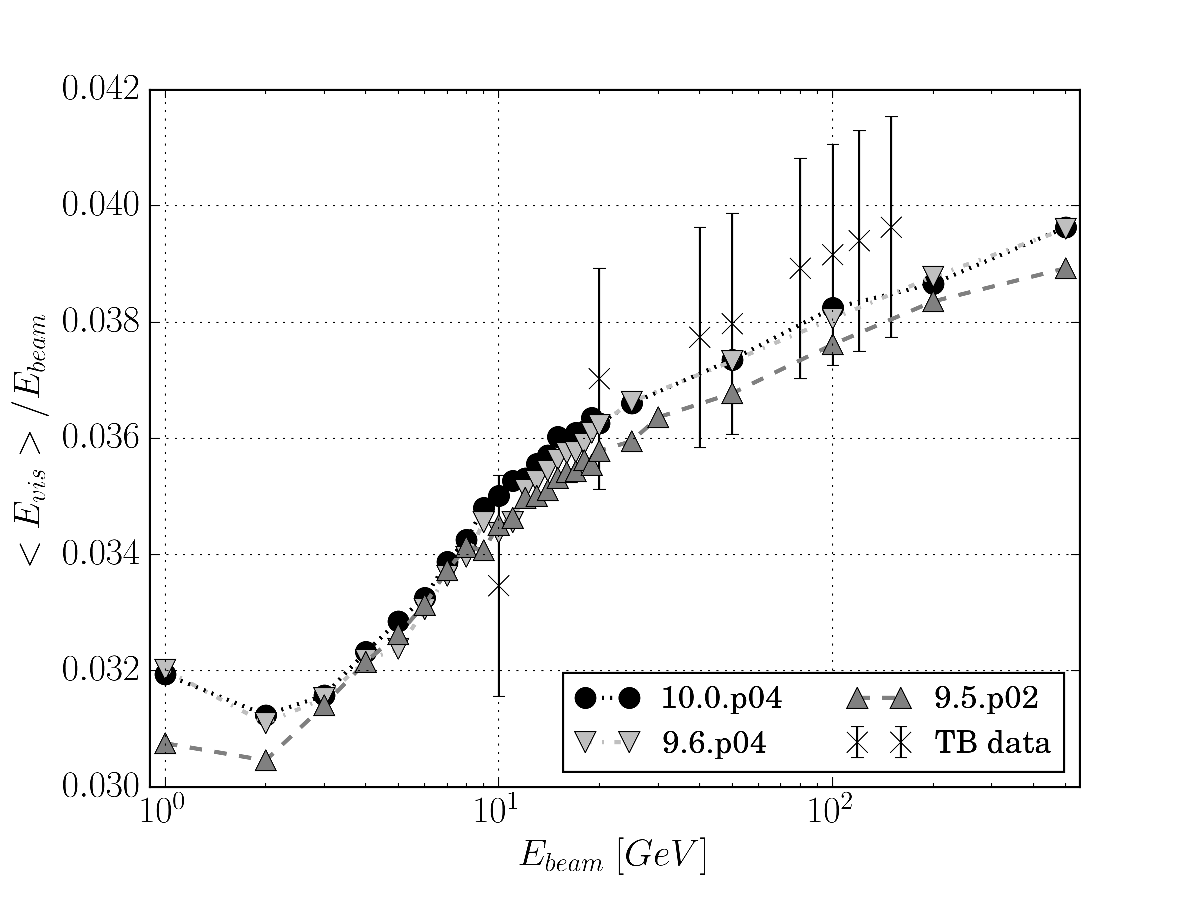
\includegraphics[width=0.5\textwidth]{figures/response.pdf}
    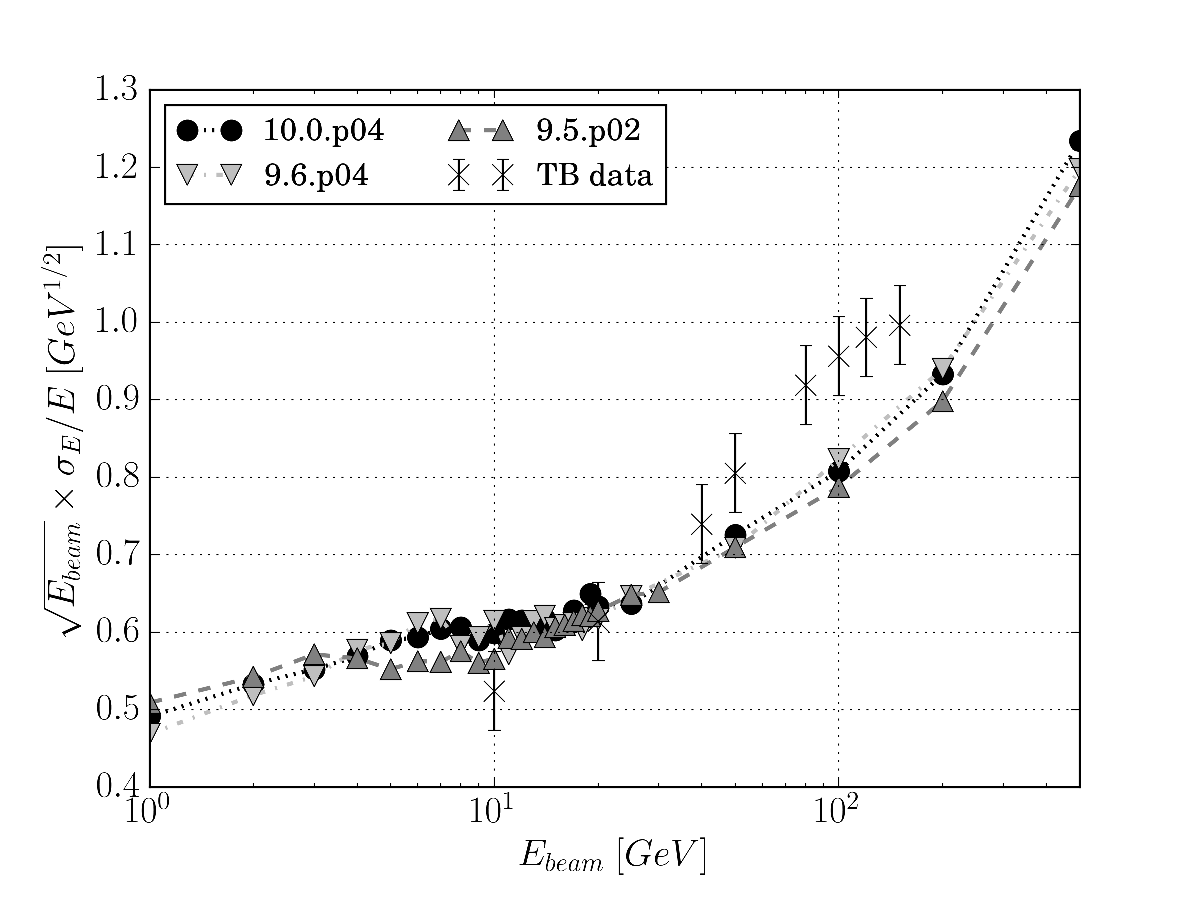
\includegraphics[width=0.5\textwidth]{figures/resolution.pdf}
   \caption{Comparison of recent \Gfour{} versions with test beam data for the
            response (top) and resolution (bottom) of the copper/liquid argon
            simplified calorimeter (ATLAS HEC).}
   \label{fig:response}
 \end{center}
\end{figure}

\subsubsection{Electromagnetic showers}
Significant efforts have been made to improve the simulation of electromagnetic
shower shapes in order to describe the details of the 
$H \rightarrow \gamma\gamma$ signal~\cite{Aad20121,Chatrchyan201230} and other 
reactions.  The bremsstrahlung process and the simulation of multiple scattering
were reviewed and improved, having been identified as key components in defining
shower shapes.  Calorimeters are particularly sensitive to the simulation of 
electron and gamma transport in the MeV energy region.  Therefore a large amount
of validation and benchmarking was, and continues to be, carried out for medium
and low energy electrons and gammas down to about 1 keV.  For these validation 
studies data from numerous thin-target and calorimeter test-beam experiments are 
used as well as comparisons with other \Gfour{} low energy electromagnetic 
models, such as the Livermore and Penelope sub-packages, which have been 
recently adapted to a common interface (see section \ref{sec:emuni}) with the 
standard electromagnetic sub-packages~\cite{pnst-VI}.

The process of multiple scattering (MSC) of charged particles is a key component
of Monte Carlo transport codes.  At high energy it defines the deviation of 
charged particles from ideal tracks, limiting the spatial resolution of 
detectors.  The scattering of low energy electrons defines the energy flow via 
volume boundaries.  This affects the sharing of energy between absorbers and 
sensitive elements, directly affecting shower shapes.  A comprehensive 
description of recent improvements of the \Gfour{} electromagnetic module can be
found in~\cite{1742-6596-396-2-022013}.
%  The general 
Good agreement was found when \Gfour{} predictions were compared with 
experimental data collected at the LHC
% is below the percent 
%level for energy response 
~\cite{1748-0221-6-04-P04001}.
% , and at the few percent 
% level for energy resolution and shower shapes.

\subsubsection{Hadronic showers}
To increase the quality of simulations of hadronic showers three main components
are needed: a string model at high energies, a cascade model at intermediate 
energies (from few hundred~MeV up to about 10~GeV) and pre-equilibrium and 
evaporation models at low energies (below a few hundred MeV).  For these energy
ranges the Fritiof, Bertini and {\gclass G4Precompound} models, respectively, 
are recommended.

Detector response is an effective test of any model combination.  It is defined
as the ratio of deposited energy visible to the detector, to the incident beam 
energy.  For the above combination of models (as in the FTFP\_BERT physics list),
the general agreement between the simulated response and data for hadron-induced
showers is at the level of a few percent.  Other useful data, such as shower 
shapes and energy resolution are less precisely described and show agreement at
a level of 10-20\%.

Figure~\ref{fig:response} shows the comparison between the predictions of 
\Gfour{} simulations with test beam data collected by the ATLAS 
Collaboration~\cite{Kiryunin2006278}. The response to pion beams is shown as a 
function of the particle energy for different versions of \Gfour{}, along with 
a comparison of the resolutions.  Note that no contribution from electronic 
noise is simulated in this case. 

A comparison of Monte Carlo calculations for the lateral (top) and longitudinal
(bottom) dimensions of hadronic showers~\cite{1742-6596-293-1-012022} are shown 
in Figure~\ref{fig:shapes} as a function of the beam energy for different 
versions of \Gfour{}. The detailed validation against experimental data requires 
the use of highly granular calorimeters such as the ones being designed by the 
CALICE collaboration. However, preliminary results suggest that \Gfour{} hadronic
showers are too compact and short.  Comparisons with LHC test beam data has 
shown that a fundamental ingredient for improving the description of the lateral 
development of showers is the use of intermediate and low energy models that 
can describe the cascading of hadrons in nuclear matter and the subsequent 
de-excitation of the wounded nucleus. The longitudinal development of hadron 
showers mainly depends on the hadronic interactions at higher energies in the 
forward direction: quasi-elastic scattering and diffraction.

An important effect recently introduced in \Gfour{} is the improvement of the
neutron capture cross sections and final state generator.  Based on the high
precision neutron library, it allows for an improved simulation of the time 
structure and the lateral profile of hadronic showers in neutron-rich 
materials~\cite{timestructure}. Other improvements include a retuned Fritiof
model which will be made available in future \Gfour{} versions.

 \begin{figure}[htb]
 \begin{center}
    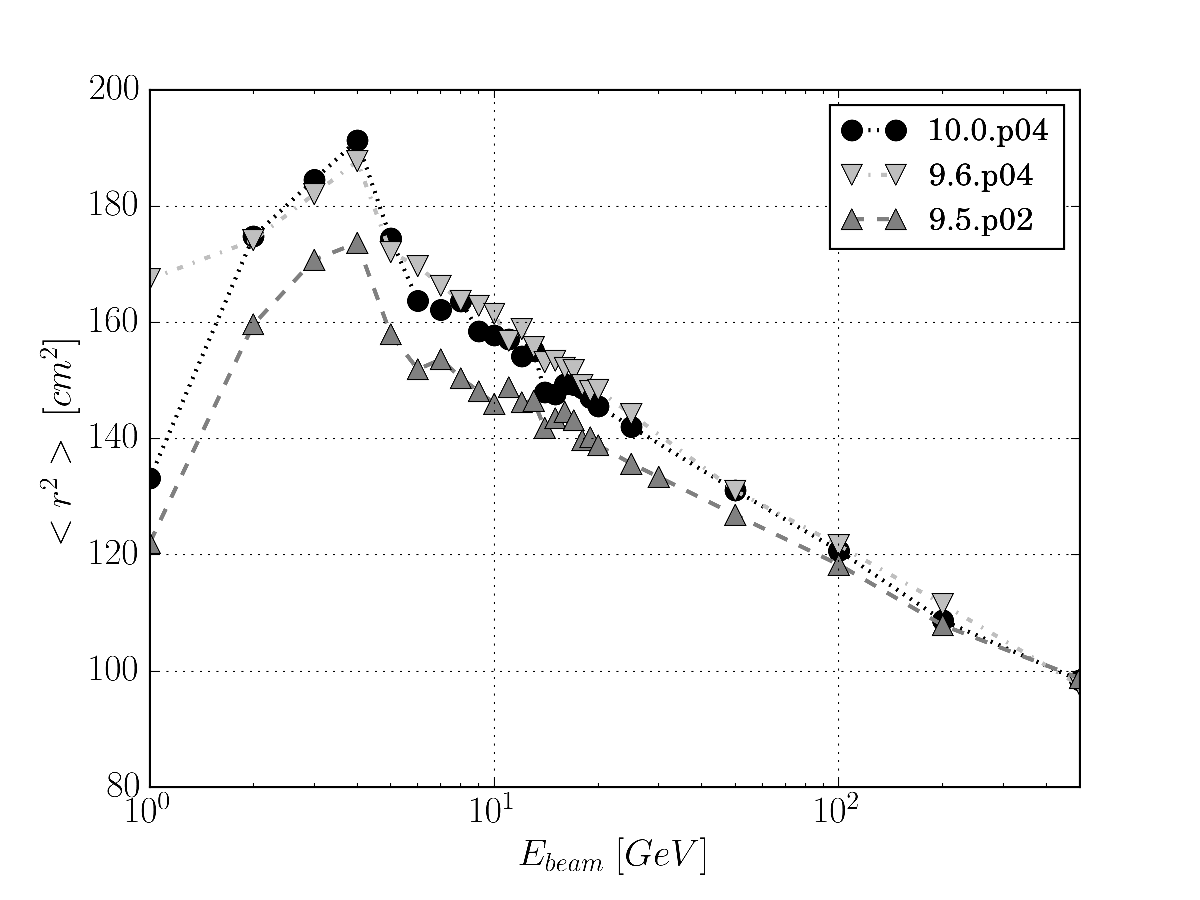
\includegraphics[width=0.5\textwidth]{figures/lateral.pdf}
    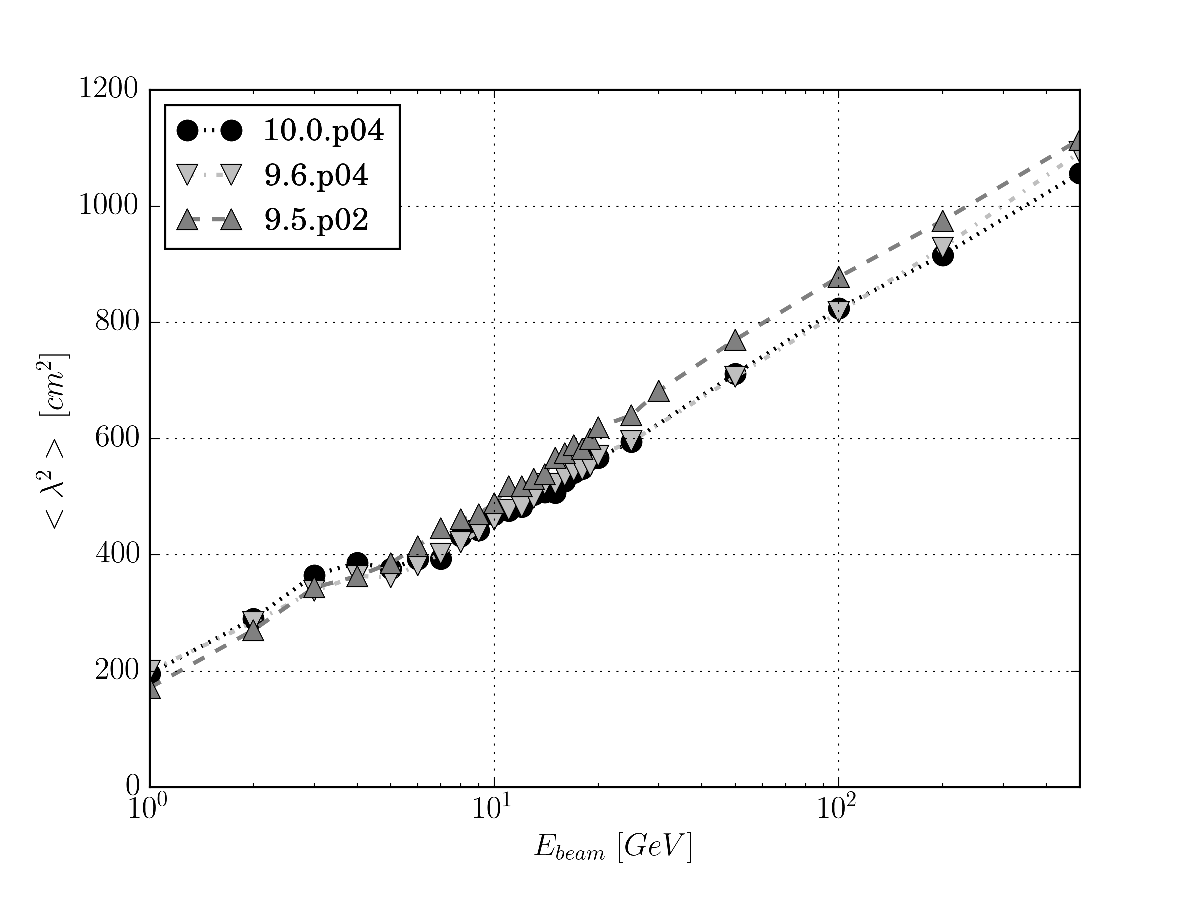
\includegraphics[width=0.5\textwidth]{figures/longitudinal.pdf}
   \caption{Comparison of recent \Gfour{} versions using the simplified
            iron/scintillator calorimeter (ATLAS TileCal).  Lateral 
            shower shapes (top) and longitudinal shower
            shapes (bottom) are shown.}
   \label{fig:shapes}
 \end{center}
\end{figure}



\section{Toolkit Extensions}

  % Authors: Marc Verderi, Pedro Arce : mostly complete
  %%%%%%%%%%%%%%%%%%%%%%%%%%%%%%%%%%%%%%%%%%%%%%%%%%%
% biasreverese.tex
%%%%%%%%%%%%%%%%%%%%%%%%%%%%%%%%%%%%%%%%%%%%%%%%%%%
\label{sec:biasreverse}

\subsection{\textbf{Biasing and reverse Monte Carlo}}\label{sec:biasrev}
There is a class of applications for which rare events are of interest, and for
% \footnote{``Event'' has to be understood in a generic sense here: 
% this is not a \gclass{G4Event}, but can be any situation of interest.}
which standard, or analog, simulation is inefficient, or even impractical.
% Note that in this context ``event'' should be understood as any occurrence of
% interest and not a \gclass{G4Event}.
Estimating shielding efficiency in a radioprotection problem is one example: an
analog simulation would spend by far most of its time transporting numerous 
particles and interaction products inside the shield, with only a tiny fraction
of particles leaving the shield.  In this case, these latter particles are the 
``rare events'' (note that in this context ``event'' should not be understood 
as a \gclass{G4Event}).  At the opposite extreme would be the simulation of very
thin detectors, which is also difficult as only a small fraction of particles 
may interact inside.  Another example is the simulation of single event upsets 
in an electronic chip within a satellite.  Here the volume of interest is very 
small compared to the overall structure in which the simulation is to be 
performed.  The events of interest (track steps in the small volume) which 
deposit energy in the chip are rare given that they occur in a fraction of time
which is of the order of the ratio of the electronic chip volume to the overall 
satellite volume.

Event biasing techniques attempt to address these problems by magnifying the 
occurrence of the rare events.  This change in the simulation is reflected in
the statistical weight associated with each particle and in the ratio of 
probabilities in the biased and analog schemes to observe the particle in the
current state.  This approach allows the simulation efficiency to be boosted 
with respect to the rare events without sacrificing the physics quality 
provided by the full, detailed Monte Carlo description.

There is a large variety of biasing techniques, but they rely mostly on two main
approaches: splitting and killing (SK) \cite{bib:SK}\cite{bib:biasGeneral} and 
importance sampling (IS) \cite{bib:ImpS}\cite{bib:biasGeneral}.

In the first approach, tracks are split (killed) as long as they approach
(recede from) the phase space region of interest.  The shielding problem can be 
addressed as follows: to compensate for the natural absorption in the shield 
material and allow a sizeable number of particles to exit the shield, the flux
is artificially regenerated by splitting particles into $n$ identical copies at
regular intervals for particles moving forward, that is, on their way toward 
exiting the shield.  At each splitting, the particle weight is divided by $n$. 
If the particles move backward, they are randomly killed with probability $1/n$,
and their weights are multiplied by $n$ if they survive.  This maintains a 
high unweighted flux, leading to workable statistics, while the weighted flux
is low, as physically expected.  In this SK approach, the physics processes
are kept unchanged.

In importance sampling, the underlying physical laws are substituted with biased
laws that favor the occurrence of rare events.  The case of a thin detector 
volume can be treated as follows: the natural exponential law is replaced by a
truncated one, limited to the track path inside the volume in order to guarantee
that the collision will occur there.  The weight acquired by the particle, or 
its interaction products, when such a forced collision occurs is the ratio of 
the two interaction probability law values at the interaction point.  Thus the 
interaction law of a physics process is modified.  The final state production 
law of the process may also be biased.

Biasing can be applied at various levels in a simulation application.  Particle
generator biasing is a simple case: the analog generator is biased to favor 
phase space regions or channels of interest.  Such generator-level biasing does 
not necessarily require the weight to be propagated through the simulation stage.
The production of rare particles in high energy physics or the generation of 
specific decay chains are examples of this case, with re-weighting of the rare 
event being applied at the analysis stage.  Such generator-level biasing is of
the IS type.  When biasing is applied after the generation stage, at tracking 
time, weight computation must be handled by the simulation engine, as it will 
evolve during the particle transport.

The biasing functionalities of \Gfour{} are presented here.  At the time of the 
previous \Gfour{} general paper \cite{bib:generalpaper2} there were three main 
biasing techniques available:
\begin{itemize}
\item the Generalized Particle Source (GPS) \cite{bib:AppDevGuide}, a versatile
      set of user commands to generate primary projectiles with various weights,
      spectra and particle types; 
\item geometry splitting and weight window \cite{bib:AppDevGuide}, a method in 
      which the user specifies weight bounds for each space-energy cell of the 
      geometry, with tracks split or killed according to these bounds;
      with an extension of the scheme \cite{detmodeling:parGeom} to handle
      cells in parallel geometries, each of these being assignable to a given
      particle type;
\item hadronic cross section biasing, which allows an overall scale factor to be
      applied to cross sections, with corresponding corrections to secondary 
      particle weights, for a few relatively rare processes. 
\end{itemize}

Since then the reverse Monte Carlo technique was introduced and work began to
extend biasing functionalities using a generic approach.  Both of these efforts
are discussed below.

\subsubsection{Reverse Monte Carlo}
Reverse Monte Carlo is a biasing technique in which the primary particles 
produced by the event generator are tracked backwards in time, acquiring 
energy along the way, to determine their statistical weight.  This technique is
especially useful in the simulation of the dose received by a small electronic
chip placed inside the large, complex structure of a satellite.  The actual 
particle source consists of highly energetic electrons, and/or protons in the 
space environment, generally modeled in the simulation as a sphere that envelops
the satellite.  In this situation the fraction of simulation steps which 
contribute to the dose in the chip for particles starting from this source is of
the order of the ratio of the chip volume to the satellite volume, and hence is
very low.

In the reverse Monte Carlo approach particle tracking begins in the vicinity of
the volume of interest, using an arbitrary distribution.  In the first stage, 
primary particles are tracked backward in time, with time-reversed physics 
processes.  Such processes and particles are referred to as ``adjoint''.  At 
each interaction, an adjoint particle acquires energy and may also change its 
type: an adjoint $e^-$ may, for example, become an adjoint $\gamma$ if an 
adjoint photo-electric process takes place.  Adjoint particles are tracked back
to their extended source.  At the end of this tracking the weight of the adjoint
particle represents the statistical weight that the full reverse track (from the
adjoint source to the external source) would have in a forward simulation.  In 
other words it represents the probability belonging to this specific track from 
the external source to the adjoint source.

The arbitrary spectrum chosen in the vicinity of the volume of interest leads 
to a biased spectrum at the source.  The statistical weight of a primary 
particle is then given by the ratio of the actual to the biased distribution 
values at the source.  Note that this weight may be zero, leading to the 
particle being ignored, if the adjoint particle has an energy which is outside 
the energy bounds of the source.  Once these weights are determined, the second 
stage begins in which particles are tracked with the usual, time-forward physics
processes, beginning from the same space-time point where the adjoint transport 
started.  The weights obtained during the reverse tracking stage allow a proper
accounting of their contribution to the dose.

\paragraph{Design}
The implementation of reverse Monte Carlo in \Gfour{} \cite{bib:revMC} was 
designed to reduce as much as possible the modifications of user code required
in order to use it.  The 
\gclass{G4Adjoint\allowbreak{}Simulation\allowbreak{}Manager} class should be 
instantiated in \texttt{main()} and the physics list should be adapted in order
to create adjoint particles (electrons, protons and gammas), and to declare 
their corresponding adjoint electromagnetic processes.  An example of such a 
physics list is given in \verb"examples/extended/biasing/ReverseMC01".

During an event in reverse simulation, pairs of adjoint and forward equivalent 
particles (same type and energy but opposite direction) are generated randomly
at the same position on a surface set by the user and containing the small 
sensitive volume considered in the simulation.  This is called the adjoint 
source.  The reverse tracking and computation of the weight of the adjoint 
particle is controlled by the reverse machinery and no user code is required
for the control of the tracking phase.  During the forward tracking phase of 
the equivalent normal particle the usual \Gfour{} actions coded by the user are 
applied in order to compute the various tallies of the simulation. 

The analysis part of the user code should be modified to normalize the signals
computed during the forward tracking phase to the weight of the equivalent
adjoint particle that reaches the external surface.  This weight represents the
statistical weight that the full reverse track (from the adjoint source to the 
external source) would have in a forward simulation.  If a forward-computed 
signal is multiplied by the weight of the reverse track and is registered as a
function of energy and/or direction it will give the response function of the 
signal.  To normalize it to a given spectrum it has to be further multiplied by
a directional differential flux corresponding to this spectrum.  The weight, 
direction, position, kinetic energy, and type of the last adjoint particle that
reaches the external source, and that would represent the primary of a forward
simulation, can be obtained by public methods of the 
\gclass{G4Adjoint\allowbreak{}SimManager}
class.  More details on how to adapt user code to use the reverse Monte Carlo 
scheme are provided in the Application Developer Guide \cite{bib:AppDevGuide}.

\paragraph{Performance}
The performance of the reverse Monte Carlo can be evaulated using the execution
time and relative precision of the results.  A useful figure of merit ($FOM$) is 
\begin{equation}
FOM = \frac{1}{R^2 T} , 
\end{equation}
where $R$ is the relative precision reached for a given execution time $T$, in
minutes.  For a typical application \cite{bib:revMC}, FOM is 4.9 for a forward
method, compared to 7600 for a reverse method.  This corresponds to a time 
speed-up factor of 1250.  Such results will of course vary depending on set-up
and physics, but it is clear that with this method, large speed-up factors can 
be achieved without sacrificing precision.    

\subsubsection{Generic Biasing}
In an attempt to unify the various forward-tracking biasing techniques, a new
scheme was introduced in release 10.0.  It aims to provide the user, through a
restricted set of base classes, flexible means to handle virtually any type
of biasing.

\paragraph{Design}
The design relies on two main abstract classes.  
\gclass{G4\allowbreak{}V\allowbreak{}Biasing\allowbreak{}Operation}
represents any type of biasing operation: splitting/killing or physics process 
modification (of the interaction law, or of the final state generation).  The 
second class, \gclass{G4VBiasingOperator}, is the decision-making entity, and 
selects the biasing operations to be applied during the current step.

A third, concrete class is \gclass{G4Biasing\allowbreak{}Process\allowbreak{}Interface}
which derives from \gclass{G4VProcess} and provides the interface between the
tracking and the biasing.  At tracking time,
\gclass{G4Biasing\allowbreak{}Process\allowbreak{}Interface} checks for a possible 
\gclass{G4VBiasing\allowbreak{}Operator} associated with the current volume.  If
such an operator exists, \gclass{G4Biasing\allowbreak{}Process\allowbreak{}Interface} 
requests the operator for biasing operations to be applied.  If no operation is 
returned, \gclass{G4Biasing\allowbreak{}Process\allowbreak{}Interface} continues
with standard tracking.

A \gclass{G4Biasing\allowbreak{}Process\allowbreak{}Interface} object can wrap a
physics process so that it controls it, and takes over the standard behavior in 
volumes where biasing is applied.  At the beginning of the step the current 
\gclass{G4VBiasing\allowbreak{}Operator} may request the 
\gclass{G4Biasing\allowbreak{}Process\allowbreak{}Interface} to apply an 
occurrence biasing operation to the physics process.  The operator may also
request \gclass{G4Biasing\allowbreak{}Process\allowbreak{}Interface} to apply a
final state biasing operation when \gclass{Post\allowbreak{}Step} process 
actions are invoked.  If a \gclass{G4Biasing\allowbreak{}Process\allowbreak{}Interface}
object does not wrap a physics process, it is meant for applying splitting/killing
biasing operations.

For the case of occurrence biasing, the problem is specified by providing
a biased interaction law, represented by the abstract class 
\gclass{G4VBiasing\allowbreak{}Interaction\allowbreak{}Law}. This is discussed
in more detail below. 

\paragraph{Occurrence biasing case}
\Gfour{} transports particles by allowing discrete interaction physics processes
to compete in producing the shortest distance to the next interaction.  Each 
distance is sampled according to an exponential law driven by the process 
``interaction length'' (inverse of cross section);  the competition makes the 
sampling equivalent to one that would be made using the total cross section.
Occurrence biasing consists in substituting some other interaction law for the
analog exponential one.  The exponential transform \cite{bib:exptran} and 
forced collision are of this type of biasing.

The weight computation relies on the following formalism.  For $N(\ell)$ 
particles present at distance $\ell$, and in the asymptotic limit of 
$N(\ell)\to \infty$, the positive number $-{\rm d}N$ of these interacting
in the next segment ${d}\ell$ is related to the cross section 
$\sigma(\ell) \ge 0$ at this position by
\begin{equation}
\label{eqn:bias_rel_loss}
\frac{-{\rm d}N}{N(\ell)}=\sigma(\ell) {{\rm d}\ell}.
\end{equation}
The quantity $\sigma(\ell) {{\rm d}\ell}$ is the one-particle probability to 
undergo an interaction in the segment $[\ell, \ell+{\rm d}\ell]$.  Note that
$\sigma(\ell)$ is not assumed to result from physical cross sections per nucleus
but rather that it is a simple function of $\ell$, referred to here as an
``effective cross section''.  Making $-{\rm d}N$ proportional to $N(\ell)$
in~(\ref{eqn:bias_rel_loss}) assumes that tracks are independent of each other.
Also, only a dependence on $\ell$, and on no previous coordinates, is considered
in~(\ref{eqn:bias_rel_loss}) in order for $N$ and $\sigma$ to describe the 
interaction probability in the next segment ${d}\ell$; this assumes the 
transport is of Markov nature.  Our biasing scheme is based on these two 
fundamental assumptions.

%For a neutral particle in a uniform medium, the physical cross section is 
%independent of $\ell$, and $\sigma(\ell) \equiv \sigma^{\rm neutral}_\phi$, 
%where $\sigma^{\rm neutral}_\phi$ is the macroscopic cross section in this medium.
%Its value changes only after an elastic interaction.  In contrast, as will be shown
%below, a biased scheme generally leads to an effective cross section which
%depends on $\ell$ and changes its value even in the absence of an interaction.

%The case of a charged particle in a uniform medium is more delicate as the 
%genuine dependence of the cross section is on the particle energy.  The particle
%energy evolves during the transport between collisions because of energy loss,
%which is the cumulative effect of a long series of small elastic (in the center
%of mass) interactions, or because of acceleration by an electric field, for
%example.  Thus $\sigma(\ell) \equiv \sigma^{\rm charged}_\phi(E(\ell))$.  One 
%complication is that $E(\ell)$ is not a unique function, valid for all particles
%initially in the same state at $\ell = 0$, but has fluctuations due to each 
%particle having its own history.


For a neutral particle in a uniform medium, the physical cross section is 
independent of $\ell$, and the effective cross section is simply
$\sigma(\ell) \equiv \sigma^{\rm neutral}_\phi$, 
where $\sigma^{\rm neutral}_\phi$ is the macroscopic cross section in this medium.
Its value changes after an elastic interaction, as the projectile energy changed.
The case of a charged particle in a uniform medium is more delicate
as the particle energy evolves during the transport because of energy loss,
or by application of an electric field, for example.
The effective cross-section evolves as
$\sigma(\ell) \equiv \sigma^{\rm charged}_\phi(E(\ell))$,
where $\sigma^{\rm charged}_\phi$ is the macroscopic cross section, the
complication being that $E(\ell)$ is not a unique function but depends on
each particle history.

In a biased scheme, such as the forced collision the effective cross section may
evolve with $\ell$ even for the case of a particle of constant energy.\\

Integrating~(\ref{eqn:bias_rel_loss}), leads to
\begin{eqnarray}
N(\ell) &=& N(0)\cdot \exp\left(-\int_0^\ell {\sigma(s){\rm d}s}\right) \nonumber \\
        &=& N(0)\cdot P_{NI}(0\to\ell),
\end{eqnarray}
where $P_{NI}(0\to\ell) \equiv \exp\left(-\int_0^\ell {\sigma(s){\rm d}s}\right)$
is the non-interaction probability from the origin to distance $\ell$,
% The right term factor $\exp\left(-\int_0^\ell {\sigma(s){\rm d}\ell}\right)$ is
% the fraction of particles free of interactions at distance $\ell$.
% For a single particle, it is the non-interaction probability from the origin to
% distance $\ell$
% \begin{eqnarray}
% \label{PNI_def}
% P_{NI}(0\to\ell) &\equiv& \exp\left(-\int_0^\ell {\sigma(s){\rm d}s}\right),
% \end{eqnarray}
%which is a monotonic decreasing function, as it must be for a non-interaction probability.
and is a monotonic decreasing function, as it must be for a non-interaction probability.
%

%The Markov nature in the differential 
%equation~(\ref{eqn:bias_rel_loss}) is visible in $P_{NI}(0\to\ell)$: if the 
%particle makes an initial step $0\to\ell_1$, followed by a second step
%$\ell_1\to\ell$, with no interaction, $\sigma(\ell)$ is the same function 

The Markov nature of Eq.~(\ref{eqn:bias_rel_loss}) is reflected in 
$P_{NI}(0\to\ell)$: if considering a particle making an initial step $0\to\ell_1$,
followed by a second step $\ell_1\to\ell$, with no interaction,
%
then
$P_{NI}(0\to\ell_1)P_{NI}(\ell_1\to\ell) = P_{NI}(0\to\ell)$,
%
% In an actual Monte Carlo, coordinates for the second step $\ell_1\to\ell$ will
% indeed be changed such that this step will be $0\to\ell-\ell_1$, with the proper
% translation of the cross section function changed:
% $\sigma(s) \to \sigma^\prime(s) \equiv \sigma(\ell_1+s), \forall s \ge 0$.
% For simplicity this shift is not shown in Eq.~(\ref{PNI_def}), which remains 
% numerically the same.
%
% Thus
% \begin{eqnarray}
% \label{PNI_markov}
% P_{NI}(0\to\ell_1)P_{NI}(\ell_1\to\ell) &=& \exp\left(-\int_0^{\ell_1} {\sigma(s){\rm d}s}\right) \exp\left(-\int_{\ell_1}^\ell {\sigma(s){\rm d}s}\right), \nonumber \\
% &=& P_{NI}(0\to\ell),
% \end{eqnarray}
and the probability in $\ell$ does not depend on the previous steps made. This
shows that a biased scheme can still follow a competitive approach between
processes, whether biased and/or non-biased.  The particle flight can be
interrupted at any distance, and non-interaction probabilities in both biased
and analog schemes will be well-defined.

If $p(\ell)$ is the probability density function of interactions, it is related 
to the non-interaction probability by:
\begin{equation}
\label{eqn_PNI_p}
P_{NI}(0\to\ell) = 1 - \int_0^\ell {p(s){{\rm d}s}} ,
\end{equation}
which conversely leads to
\begin{equation}
\label{eqn:p_to_PNI}
p(\ell) = -\frac{{\rm d}}{{\rm d}\ell}P_{NI}(0\to\ell) = \sigma(\ell) P_{NI}(0\to\ell) .
\end{equation}
%Using relation~(\ref{PNI_def}),  equation~(\ref{eqn:p_to_PNI}) can be recast as
%\begin{eqnarray}
%p(\ell) &=& \sigma(\ell) \exp\left(-\int_0^\ell {\sigma(s){\rm d}\ell}\right), \label{eqn:p_to_sigma}
%\end{eqnarray}
%which is also
%\begin{equation}
%\label{eqn:p_to_sigma_PNI}
%p(\ell) =  \sigma(\ell) P_{NI}(\ell).
%\end{equation}
% This has a physical interpretation: 
This shows that the probability 
$p(\ell){\rm d}\ell = P_{NI}((0\to\ell)\cdot \sigma(\ell){\rm d}\ell$
that a particle interacts within the segment ${\rm d}\ell$ at distance $\ell$ is
the product of the probability that it travels $\ell$ without interaction, 
$P_{NI}(0\to\ell)$, and the probability $\sigma(\ell){\rm d}\ell$, that it 
then interacts in the segment ${\rm d}\ell$ \cite{bib:MCNP}.

$\sigma(\ell)$ can also be expressed using $p(\ell)$ and $P_{NI}(0\to\ell)$ 
using
%(\ref{eqn:p_to_sigma_PNI}) and 
(\ref{eqn:p_to_PNI})
\begin{eqnarray}
\label{eqn:sigma_to_PNI}
 \sigma(\ell) &=& -\frac{{\rm d}}{{\rm d}\ell}\log P_{NI}(0\to\ell),
\end{eqnarray}
which is positive, as it must be, as $P_{NI}(0\to\ell)$ is decreasing.
Providing any of the three functions $\sigma(\ell)$, $p(\ell)$ or $P_{NI}(0\to\ell)$
is enough to define the problem.

If several biased independent processes $(i), i=1\dots n$, with effective
cross sections  $\sigma^{(i)}(\ell)$, contribute to particle interactions, each
one is responsible for an interaction amount $-{\rm d}N^{(i)}$ in a segment 
${\rm d}\ell$.  These numbers add up, and Eq.~(\ref{eqn:bias_rel_loss}) 
becomes
\begin{equation}
\label{eqn:bias_rel_loss_many}
\frac{-\sum_i{\rm d}N^{(i)}}{N(\ell)}=\sum_i\sigma^{(i)}(\ell)\cdot {{\rm d}\ell}.
\end{equation}
Equation~(\ref{eqn:p_to_PNI})
%~(\ref{eqn:p_to_sigma_PNI})
keeps the same form, with $\sigma(\ell)$ and
$P_{NI}(0\to\ell)$ becoming the total effective cross section and 
non-interaction probability, given by
\begin{eqnarray}
\sigma(\ell) &=& \sum_i\sigma^{(i)}(\ell), \\
P_{NI}(0\to\ell) &=& \prod_i P^{(i)}_{NI}(0\to\ell).
\end{eqnarray}

A scheme has been implemented in which discrete interaction physics processes
can be biased independently of each other, each possibly having its analog 
interaction law replaced by a biased one. The related analog and biased 
quantities will be denoted by subscripts $a, b$, or by superscripts $(a), (b)$, 
respectively.

In a step, any process which looses the competition for the distance to the next
interaction ends up with a non-interaction.  The biased and analog versions of 
the same process $(i)$ have different probabilities for this to occur, which is
reflected by multiplying the track weight by a non-interaction weight for
each process, and which is
\begin{eqnarray}
\label{eqn:non_int_weight}
w_{NI}^{(i)}(0\to\ell) &\equiv& \frac{P^{(i)}_{NI;\,a}(0\to\ell)}{P^{(i)}_{NI;\,b}(0\to\ell)} .
\end{eqnarray}
For the process which wins the race, the total weight to be applied is
\begin{eqnarray}
w_{\rm total}^{(i)}(\ell) &=& \frac
{p^{(i)}_a(\ell){\rm d}\ell}
{p^{(i)}_b(\ell){\rm d}\ell} , \nonumber \\
&=& w_{NI}^{(i)}(0\to\ell)\cdot w_{I}^{(i)}(\ell) ,
\end{eqnarray}
where $w_{I}^{(i)}(\ell)$ is called the interaction weight, given by
\begin{eqnarray}
\label{eqn:int_weight}
w_{I}^{(i)}(\ell) &\equiv& \frac
{\sigma^{(i)}_a(\ell)}
{\sigma^{(i)}_b(\ell)} .
\end{eqnarray}
Even for this process, it is seen that the non-interaction weight is involved.

In summary, for a track taking a step of length $\ell$, each process $(i)$
multiplies the track weight by its non-interaction weight $w_{NI}^{(i)}(\ell)$~\cite{bib:Weller};
in addition, the process winning the competition for the distance to the next
interaction further multiplies the track weight by its interaction weight 
$w_{I}^{(i)}(\ell)$.\\

The design of occurrence biasing relies on the 
\gclass{G4VBiasing\allowbreak{}Interaction\allowbreak{}Law} class
% §§ ->>>
which defines an abstract interface to model interaction laws.
The $P^{(i)}_{NI}(0\to\ell)$ and $\sigma^{(i)}(\ell)$ calculations are to be
provided by overriding, respectively, the pure virtual methods
% §§ <<<-
\begin{itemize}
\item \gclass{G4double ComputeNonInteraction\allowbreak{}ProbabilityAt(G4double l)} and
\item \gclass{G4double ComputeEffective\allowbreak{}CrossSectionAt(G4double l)},
\end{itemize}
% §§ where \gclass{l} is the length of the step taken.
where \gclass{l} is a re-notation of the length $\ell$ of the step taken.

For a physics process $(i)$ under the control of a 
\gclass{G4\allowbreak{}Biasing\allowbreak{}Process\allowbreak{}Interface} 
instance $(I)$, $(I)$ collects the process cross section at the beginning of
the step and asks the current biasing operator for a potential occurrence 
biasing operation.  If such an operation is provided, it comes with a 
\gclass{G4VBiasing\allowbreak{}Interaction\allowbreak{}Law} that the operator
samples to cause $(I)$ to compete for the next interaction.  The process cross
section is used to build a version of 
\gclass{G4VBiasing\allowbreak{}Interaction\allowbreak{}Law} implementing a 
classical exponential law.  In the subsequent \gclass{Along\allowbreak{}Step}
% §§ ->>>
stage, all instances $(I)$ provide the non-interaction weight
$w_{NI}^{(i)}(0\to\ell)$ (Eq.~(\ref{eqn:non_int_weight})) of their physics process $(i)$
% §§ <<<-
using the method 
\gclass{Compute\allowbreak{}Non\allowbreak{}Interaction\allowbreak{}Probability\allowbreak{}At(l)}
of the biased and analog laws.  In the following \gclass{Post\allowbreak{}Step}
stage, if an instance $(I)$ won the next interaction race, it further applies the weight
for interaction
% §§ ->>>
$w_{I}^{(i)}(\ell)$ (Eq.~(\ref{eqn:int_weight})) of process $(i)$
% §§ <<<-
using the
\gclass{Compute\allowbreak{}Effective\allowbreak{}Cross\linebreak[1]SectionAt(l)} 
method of the two laws.  This interaction weight multiplies the weight of all 
the final state tracks
% §§ ->>>
% §§ produced in
(primary or secondaries) issued from the interaction. This final state may
be the one of the analog versions of the physics process, or a final-state-biased
version of it.\\
% §§ <<<-

In release 10.0, a few concrete occurrence biasing functionalities were provided.
The class \gclass{G4BOptnChangeCrossSection} is a biasing operation to change a
process cross section.  Given this change can be done per process and on a 
step-by-step basis, it can be used to implement schemes similar to the 
exponential transform \cite{bib:exptran}.

The class \gclass{G4BOptrForceCollision} is a biasing operator that reproduces
the forced collision scheme of MCNP \cite{bib:MCNP}.  It handles several 
biasing operations to achieve this: a splitting operation to make a copy of the
track entering the volume, an operation to force the primary track to cross the
volume without interaction (and no tally) and update its weight accordingly, 
and an operation to force the collision on the primary clone, using the total 
interaction cross section collected from the physics processes.

These two schemes have been validated on neutral tracks.



  % Author: Pedro Arce
  %%%%%%%%%%%%%%%%%%%%%%%%%%%%%%%%%%%%%%%%%%%%%%%%%%%
% errorprop.tex
%%%%%%%%%%%%%%%%%%%%%%%%%%%%%%%%%%%%%%%%%%%%%%%%%%%
\label{sec:errorprop}

\subsection{\textbf{Error Propagation}}

The track error propagation package serves to propagate one particle together 
with its error from a given trajectory state (i.e. position and momentum with
errors) until a user-defined target is reached (a surface, volume or given
track length).  Its main use is for the track fitting of simulated or real data
to reconstruct the trajectory of a particle that has left several detector
signals along its path. 

To do its work, this package uses \Gfour{} geometry and physics, so that the 
same geometry and magnetic field used in the simulation can be used for the 
track error propagation.  The \Gfour{} physics equations can also be used, but
it is the average trajectory that should be propagated and this must be taken 
into account.  Although the user may use his/her own physics list, a physics 
list provided in the package is recommended.  It has no straggling due to 
multiple scattering, no fluctuations in the energy loss, no emission of 
secondary particles and no hadronic processes.  This physics list also 
accommodates backward propagation as well as forward (the direction the track 
followed to produce the detector signals).

When a track is propagated forward, it loses energy and the energy at the 
beginning of the step is used to calculate the energy loss.  When a track is
propagated backward, it gains energy and the energy at the end of the step is
used.  Thus, depending on propagation direction, quite different values of the
energy loss might be obtained.  To avoid this, the algorithm uses in both cases
the average energy to compute the energy loss.

Propagation is terminated when one of the following targets are met:
\begin{itemize}
\item \emph{Surface}: a user-defined surface is reached.  The surface does not
      have to be part of the geometry, as the propagation takes into account 
      both the geometry and the user-defined surfaces at the same time.  
      Currently plane and cylindrical surfaces may be defined, as well as
      surfaces formed from the combination of the two;
\item \emph{Volume}: the surface of one of the logical volumes of the geometry
      is reached.  The user may choose if the track is to stop only when 
      entering the volume, exiting the volume, or in both cases.
\item \emph{Track length}: a given track length is reached.
\end{itemize}

This package was implemented following GEANE~\cite{errprop:geane} from GEANT3,
which was based on the equations developed by the EMC 
collaboration~\cite{errprop:emc}. 

Users may implement the example provided with the \Gfour{} distribution, at 
\verb"examples/extended/errorpropagation".  The geometry in this example 
simulates a simplified typical high energy physics detector consisting of
\begin{itemize}
\item  an air-filled beamline,
\item  an air-filled central detector, 
\item  a copper calorimeter, divided into four sections,
\item  an aluminium calorimeter, divided into ten sections, and
\item  an air-filled muon detector.
\end{itemize}
While the example does not pretend to have a fully realistic geometry, it is 
sufficient to test the code.  Also the volumes were chosen to match those of
the example in the GEANE paper so that a detailed comparsion of results could
be done.
  
The detector is immersed in a magnetic field with a default value of 1 kilogauss
pointing along the negative $z$ axis.  This value can be changed by user command.
An initially free trajectory state is created to simulate a muon track of 20 GeV
along the $x$ axis.  This track is propagated until one of the termination 
targets mentioned above is reached.  An enviroment variable serves to select the
type of target.  Another enviroment variable allows either forward or backward 
propagation to be selected.  The user also has the freedom to choose whether
control will be returned to the user after each step, or only after the 
propagation target has been reached.



  %%%%%%%%%%%%%%%%%%%%%%%%%%%%%%%%%%%%%%%%%%%%%%%%%%%
% analysis.tex
%%%%%%%%%%%%%%%%%%%%%%%%%%%%%%%%%%%%%%%%%%%%%%%%%%%
\label{sec:analysis}

\subsection{\textbf{Analysis}}

\subsubsection{Introduction}
% History (AIDA based analysis)
% g4tools and new Geant4 analysis category
Analysis tools based on AIDA (Abstract Interfaces for Data Analysis) 
\cite{analysis:AIDA} have been used in \Gfour{} examples since release 3.0 in
December 2000, but until 2010 no analysis code was provided in the \Gfour{} 
source.  Several AIDA-compliant tools are available, including JAS, iAIDA, 
Open Scientist Lab and rAIDA \cite{bib:AppDevGuide} .
%  \cite{analysis:ApplicationDeveloperGuide}.
However some of them have not been maintained, some do not implement the AIDA
interfaces completely and some are not always easy to install and use.

A new analysis package based on g4tools~\cite{analysis:tools} was added in
\Gfour{} release 9.5 with the aim of providing users with a ``light-weight'' 
analysis tool available as part of the \Gfour{} installation without the need to 
link to an external analysis package.  It consists of the analysis manager 
classes and also includes the g4tools package.

g4tools provides code to write histograms and ntuples in several formats: 
ROOT~\cite{analysis:Root}, XML 2040 AIDA~\cite{analysis:AIDA} and CSV 
(comma-separated values) for ntuples and HBOOK~\cite{analysis:HBOOK}. It
is a part of the highly portable inlib and exlib~\cite{analysis:tools} 
libraries, which also include other facilities like fitting and plotting.  These
libraries are used to build the ioda application, available on all interactive
platforms so far, including iOS and Android, and able to read the file formats 
written with g4tools.   

The analysis classes provide a uniform, user-friendly interface to g4tools and 
hide from the user the differences between various output technologies.  They 
take care of higher level management of the g4tools objects (files, histograms
and ntuples), handle allocation and removal of the objects in memory and provide
the methods to access them via indexes.  For simplicity of use, all user 
interface analysis functions are provided within a single class which is seen by
the user as \gclass{G4AnalysisManager}.  Internally, this type is defined using
a \verb"typedef" and it can point to one of four type-specific output manager 
classes: \gclass{G4}\emph{Type}\gclass{AnalysisManager} where \emph{Type} can be 
\emph{Csv}, \emph{Root}, \emph{Xml} or \emph{Hbook}.

\subsubsection{Histogramming}
At present, one-dimensional and two-dimensional histograms are supported.  The 
properties of histograms already created can be changed with the use of
dedicated \texttt{Set()} functions including a limited set of parameters for 
histogram plotting. 

\gclass{G4AnalysisManager} also provides extensions to g4tools suitable for 
\Gfour{} applications.  Users can choose units and functions which are then 
automatically applied to filled values, a binning scheme (linear or logarithmic)
and an ASCII option which activates the printing of histograms to an ASCII file.
The activation option allows the user to activate only selected histograms.  
When this option is selected, only the histograms marked as activated are 
returned, filled or saved in a file. 

Histograms may also be created and modified interactively or in a macro 
using the rich set of commands defined in the \gclass{G4AnalysisMessenger} class.

\subsubsection{Ntuples}
Ntuples with \emph{int}, \emph{float} and \emph{double} column types are 
supported.  Depending on the selected output format, more files can be 
generated when more than one ntuple is defined in a user application.  This is
the case for XML and CSV, which do not allow writing more than one ntuple to a
file.  The ntuple file name is then generated automatically from the base file
name and the ntuple name.

\subsubsection{Multithreading}
Like all other \Gfour{} components, the analysis code was adapted for 
multithreading.  In multithreading mode, instances of the analysis manager 
are internally created on the master and worker threads and data accounting is 
processed in parallel on worker threads.  The migration to multithreading 
requires no changes in the user's client analysis code.  HBOOK output is not 
supported in multithreading mode.

Histograms produced on worker threads are automatically merged on the call to 
\verb"Write()" and the result is written to a master file.  Ntuples produced on
worker threads are written to separate files, the names of which are generated 
automatically from a base file name, a thread identifier and eventually also an
ntuple name.  No merging of ntuples is performed in order to avoid an associated 
time penalty. 

 

  %%%%%%%%%%%%%%%%%%%%%%%%%%%%%%%%%%%%%%%%%%%%%%%%%%%
% examples.tex
%%%%%%%%%%%%%%%%%%%%%%%%%%%%%%%%%%%%%%%%%%%%%%%%%%%
\label{sec:basicexamples}
\subsection{\textbf{Basic Examples}}
The \Gfour{} toolkit includes several fully coded examples which demonstrate the 
implementation of the user classes required to build a customized simulation.
The previous ``novice'' set of examples, oriented to beginning users, was 
refactored into ``basic'' and ``extended'' example sets in \Gfour{} 10.0.

The new ``basic'' examples cover the most typical use-cases of a \Gfour{} 
application while maintaining simplicity and ease of use.  They are provided as 
starting points for new application developers.  There are currently five such
examples, some of which include several options or sub-examples.  The features
demonstrated in each example will be presented in the following subsections.

All basic examples have been migrated to multithreading (MT) and no special 
steps are required to build them in this mode.  They will automatically run as
MT when they are built on the \Gfour{} libraries built with MT mode activated; 
otherwise they will run in sequential mode.  MT mode may be chosen by creating 
\gclass{G4MTRunManager} instead of \gclass{G4RunManager} in the \gclass{main()}
of the example.

% If the example is invoked in interactive mode, that is, without specifying a
% macro file on the command line, an interactive session will be established
% depending on the build options and \verb"~/.g4session".  For more details on
% this see the Application Developers' Guide \cite{bib:AppDevGuide}.  The most 
% advanced session possible will be instantiated.

% All basic examples include a macro \verb"vis.mac" that is invoked in interactive
% mode if the user builds with visualization.  It establishes a default viewer, 
% the most advanced available with the chosen session, a viewing angle, etc., 
% suitable for each example. In particular \verb"B1/vis.mac" demonstrates several
% features of the visualization system, namely the viewing style, the type and 
% appearance of trajectories, the ability to add axes, text, date and time, event
% number, the \Gfour{} logo and the ability to set the visibility of individual 
% volumes.  These are just a few of the features available with the \Gfour{} 
% visualization system \cite{bib:visprogress}.  A comprehensive list, with 
% guidance, can be found in Chapter 7 of the Application Developers Guide 
% \cite{bib:AppDevGuide}.

Basic examples can be run in interactive mode with visualization, or in 
batch mode.  The most suitable visualization parameters, such as a viewing 
angle, are selected for each example in order to promote a better understanding
of the example scenario and to demonstrate the most useful features of the 
visualization system.  A comprehensive list of visualization features can be 
found in Chapter 7 of the Application Developer Guide \cite{bib:AppDevGuide}.

\subsubsection{Example B1}
\verb"examples/basic/B1" demonstrates a simple application in which user actions
control the accounting of the energy deposit in volumes.  The dose in a selected 
volume is then calculated.  The geometry setup is defined with the use of 
simple placements (\gclass{G4PVPlacement}) and the physics is defined with the 
use of the QBBC pre-packaged physics list.  Scoring is implemented directly 
in the user action classes and an associated ``run'' object (\verb"B1Run")
is created.

This example also demostrates several features of the visualization system not
shown in other examples, namely the type and appearance of trajectories, the 
ability to add axes, text, date and time, event number, the \Gfour{} logo and
the ability to set the visibility of individual volumes.
  
\subsubsection{Example B2}
\verb"examples/basic/B2" simulates a simplified fixed target experiment. Two 
geometry setup options are provided: one using simple placements 
(\gclass{G4PVPlacement}) and one using parameterized volumes 
(\gclass{G4PVParameterisation}).  In addition a global, uniform, transverse 
magnetic field can be applied using 
\gclass{G4Global\allowbreak{}MagField\allowbreak{}Messenger}.  The physics setup
is defined using the FTFP\_BERT pre-packaged physics list with a step limiter.
Scoring is implemented with sensitive detectors and hits.

\subsubsection{Example B3} 
\verb"examples/basic/B3" simulates a simplified positron emission tomography
system.  The geometry is defined with simple placements and rotations.  A 
modular physics list is used.  Primary particles are $^{18}$F ions randomly 
distributed within a volume inside a simulated patient, with an associated 
radioactive decay process.  Scoring is implemented with \Gfour{} primitive 
scorers.

\subsubsection{Example B4}
\verb"examples/basic/B4" simulates a sampling calorimeter.  The geometry is 
defined using simple placements and replicas (\gclass{G4PVReplica}).  A global,
uniform, transverse magnetic field can be applied using 
\gclass{G4Global\allowbreak{}MagField\allowbreak{}Messenger}.
Physics is defined using the FTFP\_BERT reference physics list.

Energy deposits and track lengths of the charged particles are recorded event
by event in the absorber and gap layers of the calorimeter.  This example 
demonstrates four different scoring methods: user actions, user-developed 
objects, sensitive detectors and hits, and primitive scorers.

Also demonstrated is the use of \Gfour{} analysis tools for accumulating
statistics and computing the dispersion of the energy deposit and track lengths 
of the charged particles.  The resulting one-dimensional histograms and an 
ntuple are saved in an output file, which has ROOT format by default, but can
be changed at compilation time to other formats supported by g4tools (AIDA XML,
CSV for ntuples, or HBOOK). 

\subsubsection{Example B5}
\verb"examples/basic/B5" simulates a double-arm spectrometer with wire chambers,
hodoscopes and calorimeters. The geometry setup, less trivial than in previous 
examples, is defined using placements, rotations, replicas and a parameterization.
In addition a global, uniform, transverse magnetic field can be applied using 
\gclass{G4GlobalMagFieldMessenger}.  The physics setup is defined with the 
FTFP\_BERT reference physics list with a step limiter.  Scoring within wire 
chambers, hodoscopes and calorimeters is implemented with sensitive detectors 
and hits. 

\gclass{G4GenericMessenger} is used to define user interface commands specific 
to the user application and \Gfour{} analysis tools are used to output scoring
quantities in one-dimensional and two-dimensional histograms and an ntuple. 


\section{Validation}
  % Authors: Gunter Folger, Gabriele Cosmo
  %%%%%%%%%%%%%%%%%%%%%%%%%%%%%%%%%%%%%%%%%%%%%%%%%%%
% releasetools.tex
%%%%%%%%%%%%%%%%%%%%%%%%%%%%%%%%%%%%%%%%%%%%%%%%%%%
\label{sec:releasetools}
\subsection{\textbf{Release tools}}

%Release Process
%Introduction to release tools describing the release process.
%%%%%%%%%%%%%%%%%%%%%%%%%%%%%%%%%%%%%%%%%%%%%%%%%%%
% releaseprocess.tex
%%%%%%%%%%%%%%%%%%%%%%%%%%%%%%%%%%%%%%%%%%%%%%%%%%%

\subsubsection{Release process}
The software release process is described in the \Gfour{} policy
document~\cite{release:policy}.  It has reached a rather mature state in recent
years, with few modifications or adaptations made to the tools adopted for 
development and testing.  One adaptation was required following the migration of
the source code repository to the Subversion (SVN)~\cite{release:SVN} tool.  
This involved mainly technical updates to the tools and scripts used to package
the software, consistent with most of the principles described in the original
release policy.

A new release of the \Gfour{} software is usually issued once per year, with a
Beta preview of some of the expected new features usually torwards the end
of the second quarter of the same year.



%Software Organization
%Discussion of tag database, svn.
%%%%%%%%%%%%%%%%%%%%%%%%%%%%%%%%%%%%%%%%%%%%%%%%%%%
% softwareorganisation.tex
%%%%%%%%%%%%%%%%%%%%%%%%%%%%%%%%%%%%%%%%%%%%%%%%%%%

\subsubsection{Software organization}
\Gfour{} software is structured in a directory tree with each category 
corresponding to a high-level directory.  Categories such as geometry, which
is comprised of geometry shapes and navigation, and processes, which includes 
physics interaction models, are recursively subdivided into more and more 
specialized topics.  In general the C++ classes for each topic, such as a model
describing a specific type of interaction, are maintained or developed by one 
or a few developers. 

  Collaborative software revision management is handled by the SVN tool.  During
the development process, developers are encouraged to commit frequently changes 
to the trunk of the SVN repository.  When a change within a topic or directory 
is complete, the developer creates a tag of this code; features of the tag are 
documented changes in a History file, present in each sub(sub...) directory.  
A tag may be made of low-, intermediate- or high-level directories.   
Tags are recorded in the database using SVN commit hooks on the SVN server.  The
developer can propose such tags for inclusion into future releases using a web 
interface to the tags database.  Proposed tags will then enter the testing cycle. 


%Testing Tools
%Discussion of CDASH, CTEST, Electric Commander, distributed effort with shifts.
%%%%%%%%%%%%%%%%%%%%%%%%%%%%%%%%%%%%%%%%%%%%%%%%%%%
% testingtools.tex
%%%%%%%%%%%%%%%%%%%%%%%%%%%%%%%%%%%%%%%%%%%%%%%%%%%

\subsubsection{Testing tools}
Within the release process, integration of new or modified code into reference
tags is performed.  This requires regular nightly testing of new or modified 
code against the code base on a number of different platforms.  A platform is a 
specific combination of hardware and operating system version, a specific 
version of compiler, and a set of \Gfour{}-specific build options.  This regular
testing was migrated from a custom setup to using the CMake tool suite 
\cite{release:cdash}.  

There is a continuous testing cycle and nightly test runs.  Testing on a
specific platform is performed using the CTest tool of the CMake tool suite. 
For each platform, the source code corresponding to the set of tags to be tested
is checked out using SVN, CMake is run to configure and compile the code, and 
CTest runs the tests.  More than 80 unit test codes are applied, each testing a 
specific part of \Gfour{}.  In addition most examples and several benchmarks are
exercised during testing, bringing the total number of tests run to more than 
200. The exact number varies with platform, as optional software required by 
some tests may not be available on every platform.  CMake takes this into 
account by checking the availability of optional software during configuration, 
and skipping tests where software is missing.  Finally, a summary of test 
results is uploaded to the CDash web site.
  
In addition to nightly testing, continuous testing is performed on a small 
number of platforms using a restricted set of tests.  This regularly checks for 
changes in the status of tags, including also tags proposed for testing, and 
starts a test run when needed.  This restricted testing allows for an early,
but limited check of new software giving fast feedback to developers.


%Grid Tools
%Some words. Include discussion of simplified calorimeter tests.
%%%%%%%%%%%%%%%%%%%%%%%%%%%%%%%%%%%%%%%%%%%%%%%%%%%
% gridtools.tex
%%%%%%%%%%%%%%%%%%%%%%%%%%%%%%%%%%%%%%%%%%%%%%%%%%%

\subsubsection{Grid tools}
The simplified calorimeter is a \Gfour{} application which uses simplified 
versions of LHC calorimeters and produces simulation results for beam energies
between 1 and 500 GeV.  These results are then compared to normalized real data
so that the effects of changes between different \Gfour{} versions or physics
models on physics performance may be investigated.

Acquiring accurate simulation results requires running the simplified 
calorimeter for thousands of events.  This, in conjunction with the high 
energies, makes running the application on developer PCs or even local computing
clusters impossible due to time restrictions.  This need for computing power was
met by the use of resources provided by the Worldwide LHC Computing Grid 
\cite{GT:LHCG}.  
Simplified calorimeter jobs are split into smaller fragments and sent for 
execution in various grid sites around the world.  Results are then collected 
and pushed to the validation database.  The end user, typically a developer, is 
able to run on-demand analysis tasks through an interactive web application and 
produce plots.  The current grid tools implementation is based on the DIRAC 
workload management system which is used to distribute the jobs.  A system was 
developed to support different \Gfour{} tests, examples and applications that 
are or will be executed on the grid.  \Gfour{} libraries and executables are 
made available to the sites through the \Gfour{} CernVM-FS \cite{GT:CVMFS} 
repository.  Finally ROOT is used for the results format, merging of split jobs
and on-demand analysis.



%Performance Tests
%Some words on performance monitoring and tools
%%%%%%%%%%%%%%%%%%%%%%%%%%%%%%%%%%%%%%%%%%%%%%%%%%%
% performancetests.tex
%%%%%%%%%%%%%%%%%%%%%%%%%%%%%%%%%%%%%%%%%%%%%%%%%%%

%\subsubsection{Performance Tests}
\subsubsection{Computing performance benchmarking and monitoring}

Performance evaluation and analysis are essential for monitoring the \Gfour{}
toolkit through its development cycle for expected and unexpected changes in
computing performance, and for identifying problems and opportunities for code
improvement and optimization.  All internal development monthly releases and 
public releases are profiled with a set of applications that utilize different
input event samples, physics lists, and detector configurations.  Results from
multiple runs benchmarking CPU performance and memory use are compared to those
from previous public releases and development reference releases, and posted on
a publicly available web-site \cite{tools:g4cpt}.
  
In addition to memory footprints and a full summary of call stacks, which 
includes exclusive and inclusive function path counters, a detailed call graph
analysis is made available to \Gfour{} developers for further analysis.  The set
of software tools used in the performance evaluation procedure, both in 
sequential and multithreaded modes, includes FAST~\cite{tools:FAST}, 
IgProf~\cite{tools:IgProf} and Open$\mid$Speedshop~\cite{tools:OSS}.  The 
scalability of CPU time and memory performance in a multithreaded application is
evaluated by measuring event throughput and memory gain as a function of the 
number of threads for selected event samples.


%Quality Assurance
%Discussion of Valgrind, Coverity, DRD)
%%%%%%%%%%%%%%%%%%%%%%%%%%%%%%%%%%%%%%%%%%%%%%%%%%%
% qualityassurance.tex
%%%%%%%%%%%%%%%%%%%%%%%%%%%%%%%%%%%%%%%%%%%%%%%%%%%

\subsubsection{Quality assurance}
Each software release of \Gfour{} is validated against memory management issues,
in particular run-time memory errors (overwrites, memory corruption, etc.) and 
memory leaks, through use of the Valgrind~\cite{QA:valgrind} tool.  Verification
for run-time memory errors is completely automated as part of the system 
testing nightly builds, so that results for each test included in the testing 
suite can be retrieved directly from the testing dashboard and monitored along 
with the normal development process.  Specific sessions of Valgrind runs are 
executed periodically on a selected set of tests covering a rather wide range of
physics configurations to verify the absence of memory leaks during the 
execution of a simulation run for multiple simulated events; a summary of the 
results is distributed to developers by the release coordinator, together with 
hints on where problems may originate.  Memory leak checks are usually performed
on candidate releases as part of the software release process.

The Valgrind tool is also used for detecting errors in multithreaded simulation
applications, by means of its DRD~\cite{QA:DRD} module.  DRD allows the
identification of potential data-races happening during run-time among threads,
when one or more threads try to access the same memory location without proper
locking or protection.  It also allows easy identification and debugging of
lock contention cases, when a test program may get stuck in execution.

Static code analysis is regularly applied at every development release, by 
instrumenting the entire source code with the Coverity~\cite{QA:coverity}
tool.  The list of defects identified by the tool are first analysed and then
assigned to the responsible developers for further inspection and correction.
Since 2010, when this tool was first adopted for quality assurance, almost 3000
defects (most of them not critical) have been triaged and fixed, with priority
given to cases of potentially higher impact.




\subsubsection{Distribution}
Releases and beta previews, including all data sets, are available from the
\Gfour{} download page \cite{QA:G4down} as compressed source code files and in
compiled form for Linux, MacOS and Windows.  The source code and libraries for
Linux are also available from AFS in \url{/afs/cern.ch/sw/lcg/external/geant4} 
and in CernVM-FS in \url{/cvmfs/geant4.cern.ch/geant4}.




  % Authors: Julia Yarba, Hans Wenzel, Alberto Ribon, Andrea Dotti, Witek Pokorski
  %%%%%%%%%%%%%%%%%%%%%%%%%%%%%%%%%%%%%%%%%%%%%%%%%%%
% physvaltools.tex
%%%%%%%%%%%%%%%%%%%%%%%%%%%%%%%%%%%%%%%%%%%%%%%%%%%
\label{sec:physvaltools}
\subsection{\textbf{Physics Validation Tools}}

\subsubsection{Physics Validation Procedure}
The accuracy of the \Gfour{} physics models is benchmarked regularly using thin-
and thick-target tests.  Thin-target tests allow a detailed study of specific
observables from a single physics process for a given configuration of
projectile particle type, projectile kinetic energy and target material.
A large set of published thin-target data, collected over several years, is 
used roughly once per month to validate each internal development release. 
These data can also be used for tuning some of the parameters of the physics
models.  This is particularly true for the hadronic models, many of which are 
phenomenological.

Thick-target tests are mainly based on test beam setups.  These tests allow the
assessment of the physics accuracy of \Gfour{} simulations in realistic 
configurations, which involve several physics processes and multiple energy 
scales.  A notable example is the measurement of the properties of 
electromagnetic and hadronic showers in calorimeter test beam setups which were
carried out for the preparation of the LHC experiments, and which are ongoing
for the Linear Collider detector (CALICE).

Test beam simulations are in general complex and time-consuming, and are 
therefore repeated by experimentalists only for some \Gfour{} public releases.
To get more frequent and regular feedback, \Gfour{} developers have created a
set of simplified test beam setups which are used for regression testing, that 
is, the comparison of two or more versions of \Gfour{} for any observable.  
When a statistically significant difference is detected, for instance if the 
hadronic shower becomes wider than that observed in a previous \Gfour{} version,
the code changes responsible for the difference are investigated.

\subsubsection{Physics Validation Tests}
Model development and improvement work is tightly coupled with extensive 
efforts to validate \Gfour{} physics with experimental data.  A large collection 
of tests ranges from validation at the single process level and comparison with 
thin target experimental data to the validation of complete physics lists and 
comparison with results from LHC experiments.
 
In particular, validation with thin target data is crucial in judging the 
quality of model prediction and model tuning.  Thin target validations are done
for
\begin{itemize}
\item stopping particles ($\bar{p}$, $\pi^-$, $K^{-}$, $\Sigma^{-}$, $\Omega$),
\item low energy data ($<$100 MeV) with inclusive $n$, $p$ production in $n$,
      $p$, $\gamma$ beams on nuclear targets,
\item medium energy data (100 MeV-200 GeV) that includes $n$, $p$, $\pi^+$ 
      production in p-A or $\pi^{\pm}$-A interactions,
\item high energy data ($>$ 20 GeV) for inclusive hadron production in $\pi$ or
      $p$ interactions with nuclear targets, and
\item a number of comparisons for simplified yet realistic experimental setups
      by the \Gfour{} team and LHC experimentalists.
\end{itemize}

\subsubsection{Physics Validation Repository}
As the number of regularly performed validation tests increases and the 
collection of results grows, storing them and making them available to the 
user community becomes a challenge of its own.  It was decided to organize
this material in a central repository and to make this data generally and easily
available, not only for internal collaboration use, but also for the user 
community.

The Physics Validation Repository stores data in the form of images with 
meta-data, or as the raw data points from both simulation and experiment.
Meta-data includes descriptions of the tests, lists of references describing the
origin of the experimental data, and other parameters which describe the test,
such as beam particle type, its energy or momentum, the reaction observed and 
its secondaries, and the observable that is extracted from the measurement. 

The ability to store images allowed the initial population of the database with
the available collection of existing test results.  The alternative method of 
storing raw data points allows more interactivity, and can be used for example,
in performing regression testing and model comparisons.

As shown in Figure \ref{fig:webapp}, the physics validation repository consists
of a PostgresSQL database, a Java API and a JSP web application. 
The PostgresSQL \cite{PVT:postgres} relational database stores collections of 
tests, such as images, tags, descriptions, references, and images with meta-data
or raw data points, both experimental and simulated.
% The advantage over raw data points is
%that the use can select compatible data and overlay them and compare them. 
%This allows e.g. for the comparison of different \Gfour version
%(regression testing), comparison of different available models, target 
%materials  etc. 

The Java API is based on the data access object (DAO) design pattern, which  
provides an abstract interface to the database.  Using mapping application calls
to the persistence layer enables the DAO to provide some specific data 
operations without exposing details of the database.
% It 
%separates what data accesses the application needs, in terms of 
%domain-specific objects and data types (the public interface of the DAO), 
%from how these are implemented with the database schema.

The web application \cite{PVT:home} is based on the Enterprise Edition (Java EE)
\cite{PVT:javaee} of the Java Platform, deployed on a GlassFish Application
server \cite{PVT:glassfish}.  This allows tests to be viewed and modified, new 
tests to be uploaded, and provides security and authentication to grant access 
to functions and data internal to the \Gfour{} collaboration.
 
The PrimeFaces JSF (java server faces) Framework \cite{PVT:primefaces} is used
to create interactive, modern-looking web interfaces and charting tools based
on JavaScript are used for plotting.
% jfreechart java 
% library \cite{PVT:jfreechart} or the Highcharts 
% JavaScript library 
% \cite{PVT:highcharts} is used for plotting. 
%To convert data in the database into plots we make use of the jfreechart 
%java library or to create interactive charts we use the Highcharts JavaScript
%library. 

\begin{figure}[htb]
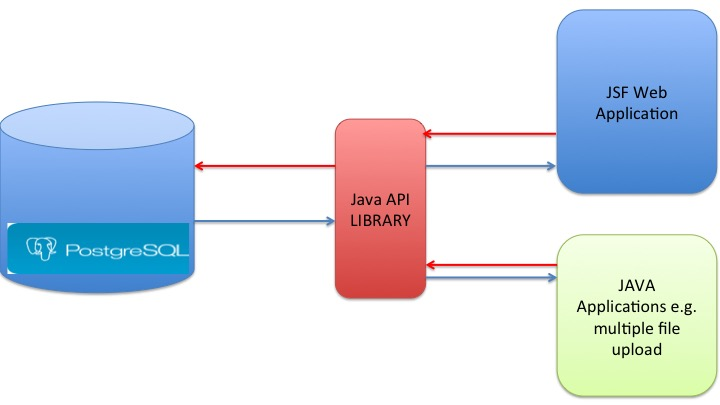
\includegraphics[width=0.45\textwidth]{figures/Components.jpg}
%  \centering
%  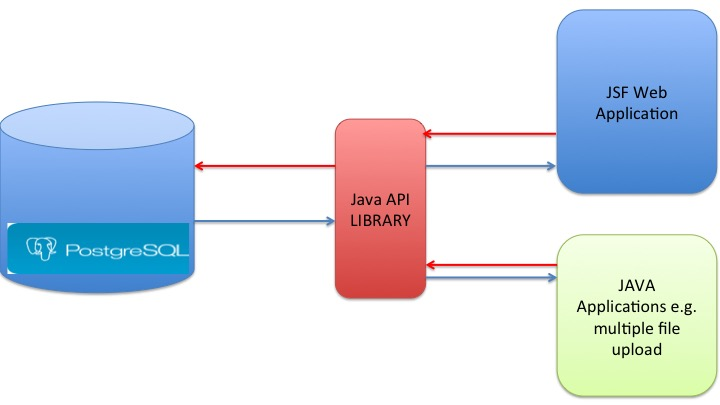
\includegraphics[width=3.4in]{figures/Components.jpg}
  \caption{Components of the \Gfour{} validation repository.} 
  \label{fig:webapp}
\end{figure}


\section{Outlook for the Next Decade}
  %%%%%%%%%%%%%%%%%%%%%%%%%%%%%%%%%%%%%%%%%%%%%%%%%%%
% outlook.tex
%%%%%%%%%%%%%%%%%%%%%%%%%%%%%%%%%%%%%%%%%%%%%%%%%%%
\label{sec:outlook}
\subsection{\textbf{A Brief Summary of \Gfour{} Progress}}
Major changes and developments in the \Gfour{} toolkit took place between the
8.1 and 10.1 releases.  These include:

\begin{itemize} 
  \item the migration to multithreading, 
%  \item the switch from gmake to CMake,
  \item the addition of tessellated solids and a unified geometry description,
  \item general biasing methods,
  \item improved and expanded physics models, 
  \item expanded validation and testing, 
  \item reference physics lists,
  \item the addition of rudimentry analysis methods, and
  \item improved and expanded visualization tools.
\end{itemize}

As a result the toolkit is more versatile, easier to use and makes more 
efficient use of available CPU and memory resources.

\subsection{\textbf{New Directions}}
These changes were made in response to the demands of a diversifying user 
community and to the opportunities made available by advancing technology.  It
is expected that both these trends will continue and that \Gfour{} will 
continue to evolve with them.

With this in mind the \Gfour{} collaboration is studying new options for the 
future.  GPUs and accelerated processors offer great potential for speeding up 
computationally intensive applications, and could possibly be adapted for use in
physics simulations.  Massively parallel computing and vectorization are also 
being examined as a way to exploit available supercomputer capacity
\cite{bib:Dotti,bib:Szo}.

The drive to make \Gfour{} easier to use will continue.  An increasing percentage
of the \Gfour{} user base requires more turn-key operation and better 
documentation.  To enable this, improved user interfaces, simplified physics  
choices and still more powerful build tools will be required.

The expansion of \Gfour{} into new physics domains will also continue. 
Users in nuclear physics require more detailed nuclear reactions and models, 
space and medical applications depend increasingly on precise, fast 
electromagnetic and radioactive decay modeling, biophysics and material 
science continue to expand the simulation of chemical kinetics and damage to 
micro-structures, and photon science is expected to be a user of radiation 
damage and accelerator dark current simulations.  While new capabilities are 
currently being developed to meet the needs of experiments at the high energy,
intensity and cosmic frontiers, it is clear that the increasing use of \Gfour{}
in other areas will also lead to new toolkit developments.



\section*{Acknowledgements}
The authors gratefully acknowledge the support of this work which has come 
directly and indirectly from many sources, too numerous to mention.  
Acknowledged as well is the generous support of experiment collaborations and
universities who have allowed their members to contribute significant time and
effort to the development, testing and validation of \Gfour{}.  The authors also
express appreciation of the users of \Gfour{}, many of whom have contributed 
code, spotted and fixed problems and disseminated \Gfour{} throughout many 
disciplines.  Finally, the authors thank KEK for providing the funds to cover 
publication of this article.

%% The Appendices part is started with the command \appendix;
%% appendix sections are then done as normal sections
%% \appendix

%% \section{}
%% \label{}

%%
%% Following citation commands can be used in the body text:
%% Usage of \cite is as follows:
%%   \cite{key}         ==>>  [#]
%%   \cite[chap. 2]{key} ==>> [#, chap. 2]
%%

%% References with bibTeX database:

% \bibliographystyle{elsarticle-num}
% \bibliography{<your-bib-database>}

%% Authors are advised to submit their bibtex database files. They are
%% requested to list a bibtex style file in the manuscript if they do
%% not want to use elsarticle-num.bst.

%% References without bibTeX database:

\begin{thebibliography}{00}

\bibitem{bib:generalpaper2} J. Allison et al.,
                            IEEE Transactions on Nuclear Science 53, 270 (2006).

%\bibitem{MT:streit}  N. Rauschmayr and A. Streit , Reducing the Memory Footprint of Parallel
%                     Applications with KSM , in Facing the Multicore-Challenge III: Aspects
%                     of New Paradigms and Technologies in Parallel Computing; Lecture Notes
%                     in Computer Science , 48-59, 2013.

\bibitem{MT:xdong} X. Dong, G. Cooperman and J. Apostolakis, Multithreaded Geant4:
                   Semi-automatic Transformation into Scalable Thread-Parallel 
                   Software , in Euro-Par 2010 - Parallel Processing,
                   Lecture Notes in Computer Science, 6272, 287-303, 2010.

\bibitem{MT:SNA2013} S. Ahn et al., Geant4-MT : bringing multi-threading into Geant4 production,
                     in Joint International Conference on Supercomputing in Nuclear Applications
                     and Monte Carlo 2013 (SNA + MC 2013).

\bibitem{MT:TDG} Geant4 Collaboration, Toolkit Developers Guide, Chapter 2,
                 available online at http://cern.ch/geant4 .

\bibitem{MT:6154433} A. Dotti, Description of hadron-induced showers in calorimeters
                     using the Geant4 simulation toolkit, 
                     in Nuclear Science Symposium and Medical Imaging Conference
                     (NSS/MIC), 2011 IEEE , 2128-2134 , 2011

\bibitem{MT:GDML} R. Chytracek, J. McCormick, W. Pokorski and G. Santin,
%                  Geometry description markup language for physics simulation
%                  and analysis applications,
                  IEEE Transactions on Nuclear Science 53 (2006) 2892.

\bibitem{MT:collaboration2008cms} CMS Collaboration, The CMS experiment at the CERN LHC,
                                  Jinst S08004 Vol 3 (2008) 187.

\bibitem{MT:leng2002study} T. Leng, R. Ali, J. Hsieh and C. Stanton,
                           A study of hyper-threading in high-performance computing clusters,
                           Dell 6 (2002) 33.

\bibitem{MT:TBB} Intel Threading Building Blocks, 
                 \url{https://www.threadingbuildingblocks.org} .

\bibitem{MT:MPI} The Message Passing Interface standard, 
                 \url{http://www.mcs.anl.gov/research/projects/mpi/} .


%%%%%%%%%%%%%%%%%%%%%%%%%%%%%%%%%%%%%%%%%%%%%%%%%%%
% detmodeling_biblio.tex
%%%%%%%%%%%%%%%%%%%%%%%%%%%%%%%%%%%%%%%%%%%%%%%%%%%

\bibitem{detmodeling:modeler} G. Cosmo, The \Gfour geometry modeler,
         IEEE Nuclear Science Symposium Conference Record, Vol. 4 (2004) 2196.

\bibitem{detmodeling:parGeom} J. Apostolakis, M. Asai, G. Cosmo, A. Howard,
                              V. Ivanchenko and M. Verderi, Parallel geometries in
                              \Gfour: foundation and recent enhancements, 
                              Proceedings of the IEEE NSS/MIC/RTSD Conference (2008). 

\bibitem{detmodeling:regnav} P. Arce, J. Apostolakis and G. Cosmo, A technique for
                             optimised navigation in regular geometries,
                             IEEE Nuclear Science Symposium Conference Record 
                             NSS08 (2008) 857.
                
% \bibitem{detmodeling:GDML} R. Chytracek, J. McCormick, W. Pokorski and G. Santin,
%          Geometry description markup language for physics simulation and analysis applications,
%         IEEE Transactions on Nuclear Science, 53(5) (2006) 2892.

\bibitem{detmodeling:USolids} M.Gayer, J. Apostolakis, G. Cosmo, A. Gheata, J.M. Guyader and
                              T. Nikitina, New Software library of geometrical primitives for
                              modeling of solids used in Monte Carlo detector simulations,
                              Journal of Physics: Conference Series 396, no. 5, p. 052035,
                              IOP publishing, 2012.

\bibitem{bib:AppDevGuide} Geant4 Collaboration, Application Developers Guide,
                          available online at http://geant4.web.cern.ch .

\bibitem{detmodeling:Brent} R.P. Brent, ``Algorithms for Minimisation without Derivatives'',
                            Chapter 4, Englewood Cliffs, New Jersey, Prentice-Hall, 1973,
                            ISBN 0-13-022335-2.

\bibitem{detmodeling:XercesC} Apache Xerces C parser,
                              \url{http://xerces.apache.org/xerces-c/} .

\bibitem{detmodeling:STEPTools} STEP Tools, Inc., open source code for 3-D object
                                representation in computer-aided design (CAD),
                                \url{http://www.steptools.com} .



%%%%%%%%%%%%%%%%%%%%%%%%%%%%%%%%%%%%%%%%%%%%%%%%%%%
% vis_biblio.tex
%%%%%%%%%%%%%%%%%%%%%%%%%%%%%%%%%%%%%%%%%%%%%%%%%%%

\bibitem{vis:Allison}
J. Allison et al.,
% The Geant4 Visualization System,
   Computer Physics Communications 178, 5, 331 (2008). 

\bibitem{vis:Qt} The Qt Project, an open source cross-platform application and
                 UI framework, \url{http://www.qt.io} .

\bibitem{vis:OGL} OpenGL, the Industry's Foundation for High Performance 
                  Graphics, \url{https://www.opengl.org/} .

\bibitem{vis:OI} OpenInventor, an object-oriented 3D toolkit offering a 
                 comprehensive solution to interactive graphics programming 
                 problems, \url{http://oss.sgi.com/projects/inventor/} .

\bibitem{vis:HPRP} HepRApp Users Home Page,
                   \url{http://www.slac.stanford.edu/~perl/HepRApp/} .

\bibitem{vis:DAWN} S. Tanaka and M. Kawaguti, DAWN for GEANT4 Visualisation, in:
                   Proceedings of the CHEP97 Conference, Berlin, April 1997,

\bibitem{vis:VRML} VRML Virtual Reality Modeling Language,
                   \url{https://www.w3.org/MarkUp/VRML/} .

\bibitem{vis:gMoc} A. Kimura, S. Tanaka, K. Hasegawa and T. Sasaki,
                   Visualization for volume data scored by Geant4 simulation,
                   IEEE Nuclear Science Symp. Conf. Record, pp. 2158-2161, 2009; \\
                   see also \url{http://geant4.kek.jp/gMocren/} .

% \bibitem{vis:OIC} Open Inventor Architecture Group,
% {\it Open Inventor C++ Reference Manual\/}, 1994.


\bibitem{vis:GL2PS} GL2PS: \url{http://guez.org/gl2ps/} .

% \bibitem{vis:Coin} Coin3D: www.coin3d.org \\

\bibitem{vis:coin3d} Coin3D, a high-level, retained-mode toolkit for effective
                     3D graphics development, 
                     \url{https://bitbucket.org/Coin3D/coin/wiki/Home} .

\bibitem{vis:polyline} Anonymous, "Distance from a Point to a Polyline",
   \url{http://programmizm.sourceforge.net/blog/2012/distance-from-a-point-to-a-polyline} . 



\bibitem{bib:G4}S. Agostinelli et al., Geant4 a simulation toolkit, 
                Nuclear Instruments and Methods in Physics Research A 506 250 (2003).
%250-303

\bibitem{bib:uni}V. Ivanchenko et al., Recent improvements in Geant4 electromagnetic physics
                 and interfaces, Progress in Nuclear Science and Technology 2 (2011) 898.

%%%%%%%%%%%%%%%%%%%%%%%%%%%%%%%%%%%%%%%%%%%%%%%%%%%
% biblio.tex
%%%%%%%%%%%%%%%%%%%%%%%%%%%%%%%%%%%%%%%%%%%%%%%%%%%

\bibitem{embib:design}J. Apostolakis et al., 
% Geometry and physics of the \Gfour{} toolkit for high and medium energy 
% applications, 
Radiation Physics and Chemistry, 78 (2009) 859.
%859-873

\bibitem{embib:dna3} M. Karamitros et al., 
% Diffusion-controlled reactions modeling in
%                      Geant4-DNA, 
                     Journal of Computational Physics 274 (2014) 841. 

\bibitem{embib:chep14} V.N. Ivanchenko et al., Geant4 electromagnetic physics for LHC 
                       upgrade, Journal of Physics: Conference Series 513 (2014) 022015.

\bibitem{embib:uni2} V.N. Ivanchenko et al., Geant4 electromagnetic physics:
                     improving simulation performance and accuracy, SNA+MC 2013 Joint 
                     International Conference on Supercomputing in Nuclear Applications
                     + Monte Carlo, p. 03101, EDP Sciences (2014).

\bibitem{embib:epdl} D. Cullen, J. H. Hubbell, L. Kissel, 
                     The evaluated photon data library, Report UCRL-50400, Vol. 6 (1997).

\bibitem{embib:pen} F. Salvat, J.M. Fernandez-Varea and J. Sempau, 
                    PENELOPE-2008: A code system for Monte Carlo simulation of electron
                    and photon transport, OECD-NEA report 6416 (2009),
                    Issy-les-Moulineaux, France.

\bibitem{embib:gamma5} A. B. Migdal,
%  Bremsstrahlung and pair production in condensed 
%                        matter at high energies, 
                       Physical Review 103 (1956) 1811.
%1811-1820

\bibitem{embib:gamma6} T. Stanev, C. Vankov, R.E. Streitmatter, R.W. Ellsworth and T. Bowen,
%                        Development of ultrahigh-energy electromagnetic cascades in water
%                        and lead including the Landau-Pomeranchuk-Migdal effect, 
                       Physical Review D 25 (1982) 1291.
%1291-1304

\bibitem{embib:gamma11} G.O. Depaola,
%  Azimuthal distribution for pair production by 
%                         high-energy gamma-rays,
                        Nuclear Instruments and Methods in Physics Research A 452 (2000) 298.
% 298-305

\bibitem{embib:gamma12} G.O. Depaola and M. L. Iparraguirre,
% Angular distribution for the electron 
%                        recoil in pair production by linearly polarized gamma-rays on electrons, 
                        Nuclear Instruments and Methods in Physics Research A 611 (2009) 84.
% 84-92
\bibitem{embib:pol3} V.F. Boldyshev, E.A. Vinokurov, N.P. Merenkov and Yu.P. Peresun'ko,
                     Physics of Particles and Nuclei 25 (1994) 3.

\bibitem{embib:pol4} M.L. Iparraguirre and G.O. Depaola,
                     European Physical Journal C 71 (2011) 1778.

\bibitem{embib:gamma13} J.M.C. Brown, M.R. Dimmock, J.E. Gillam and D.M. Paganin,
                        MULECS: The Monash University low energy Compton
                        scattering package, Nuclear Science Symposium and Medical
                        Imaging Conference (NSS/MIC) IEEE (2011) 1385.
%1385-1389

\bibitem{embib:gamma14} J.M.C. Brown, M.R. Dimmock, J.E. Gillam and D.M. Paganin,
%                        A low energy bound atomic electron Compton scattering model for Geant4,
                        Nuclear Instruments and Methods in Physics Research B 338 (2014) 77.
% 77-88

\bibitem{embib:gamma15} J.W.M. Du Mond,
% Compton modified line structure and its relation to
%                        the electron theory of solid bodies,
                        Physical Review 33 (1929) 643.
% 643-658

\bibitem{embib:gamma7} R. Ribberfors,
% Relationship of the relativistic Compton cross section to the 
%                       momentum distribution of bound electron states, 
                       Physical Review B 12 (1975) 2067.
% 2067-2074

\bibitem{embib:gamma8} Y. Namito, S. Ban and H. Hirayama,
%  Implementation of the Doppler broadening 
%                       of a Compton-scattered photon into the EGS4 code, 
                       Nuclear Instruments and Methods in Physics Research A 349 (1994) 489.
% 489-494

\bibitem{embib:gamma16} XCOM evaluated data, National Burea of Standards, \\
                        \url{http://www.nist.gov/pml/data/xcom/} .  

\bibitem{embib:gamma17}K. Amako et al.,
% Validation of Geant4 electromagnetic physics versus the
%                       NIST databases,
                       IEEE Transactions on Nuclear Science, 52 (2005) 910.
% 910-918

% \bibitem{embib:gamma17}K. Amako, S. Guatelli, V. Ivanchenko,
% M. Maire, B. Mascialino, K. Murakami, L. Pandola, S. Parlati, 
% M. G. Pia, M. Piergentili, T. Sasaki, L. Urban, Validation
% of Geant4 electromagnetic physics versus the NIST databases, 
% IEEE Transactions on Nuclear Science, 52 (2005) 910-918. 

\bibitem{embib:emmu} A.G. Bogdanov, H. Burkhardt, V.N. Ivanchenko, S.R. Kelner,
                     R.P. Kokoulin, M. Maire, A.M. Rybin and L. Urban,
%                     Geant4 simulation of production and interaction of muons,
                     IEEE Transactions on Nuclear Science 53 (2006) 513.
% 513-519

\bibitem{embib:empbar} A.V. Bagulya, M.S. Vladimirov, V.N. Ivanchenko and N.I. Starkov,
%                       Heavy-particle energy loss simulation using the Geant4 toolkit,  
                       Bulletin of the Lebedev Physics Institute 36 (2009) 127; \\
                       Original Russian Text in  
                       Kratkie Soobshcheniya po Fizike 36 (2009) 3. 
% 127-134
%  3-14

\bibitem{embib:emIon} A. Lechner, V. N. Ivanchenko and J. Knobloch, 
%                      Validation of recent Geant4 physics models for application in carbon
%                      ion therapy, 
                      Nuclear Instruments and Methods in Physics Research B 268 (2010) 14.

\bibitem{embib:fluc} K. Lassila-Perini and L. Urban, 
%                     Energy loss in thin layers in GEANT,  
                     Nuclear Instruments and Methods in Physics Research A 362 (1995) 416.

\bibitem{embib:ionfluc} Q. Yang, D.J. O'Connor and Z. Wang, 
                        Nuclear Instruments and Methods in Physics Research B 61 (1991) 149.
% 149-155

\bibitem{embib:pai} J. Apostolakis, S. Giani, L. Urban, M. Maire, M. Bagulya and V.M. Grichine, 
%                    An implementation of ionisation energy loss in very thin absorbers
%                    for the Geant4 simulation package,  
                    Nuclear Instruments and Methods in Physics Research A 453 (2000) 597.
%597-605

\bibitem{embib:chep11} A. Schaelicke et al., Geant4 electromagnetic physics for the LHC and
                       other HEP applications,
                       Journal of Physics: Conference Series 331 (2011) 032029.

% \bibitem{embib:chep11}A. Schaelicke, A. Bagulya, O. Dale, F. Dupertuis,
% V. Ivanchenko, O. Kadri, A. Lechner, M. Maire, M. Tsagri and L. Urban,
% Geant4 electromagnetic physics for the LHC and other HEP applications,
% J. Physics: Conf. Ser., 331 (2011) 032029.

\bibitem{embib:tpc1}D. Antonczyk et al., 
% Performance studies with an ALICE TPC prototype,
                    Nuclear Instruments and Methods in Physcis Research A 565 (2006) 551.
% 551-560

\bibitem{embib:tpc2}P. Christiansen,
% Particle identification studies with an ALICE test TPC,
                    International Journal of Modern Physics E 16 (2007) 2457.
% 2457-2462

\bibitem{embib:bicsel}H. Bichsel,  Reviews of Modern Physics 60 (1988) 663.
% 663-699

\bibitem{embib:dnaProc1}S. Chauvie, Z. Francis, S. Guatelli, S. Incerti, 
                        B. Mascialino, P. Moretto, P. Nieminen and M.G. Pia,
%                        Geant4 physics processes for microdosimetry simulation:
%                        design foundation and implementation of the first set
%                        of models,
                        IEEE Transactions on Nuclear Science 54 (2007) 2619.
% 2619-2628

\bibitem{embib:dnaxs} S. Incerti et al.,
% Comparison of Geant4 very low energy
%                      cross section models with experimental data in water,
                      Medical Physics 37 (2010) 4692.

%\bibitem{embib:dnaxs}S. Incerti, A. Ivanchenko, M. Karamitros, A. Mantero, 
%P. Moretto, H. N. Tran, B. Mascialino, C. Champion, V. N. Ivanchenko, 
%M. A. Bernal, Z. Francis, C. Villagrasa, G. Baldacchino, P. Guye, R. Capra, 
%P. Nieminen, C. Zacharatou,
%Comparison of Geant4 very low energy cross section models with experimental
%data in water, Medical Physics, 37  (2010) 4692-4708.

\bibitem{embib:micro} A. Valentin, M. Raine, J.-E. Sauvestre, M. Gaillardin 
                      and P. Paillet,
% Geant4 physics processes for microdosimetry
%                      simulation: very low energy electromagnetic models for 
%                      electrons in silicon,
                      Nuclear Instruments and Methods in Physics Research B 288
                      (2012) 66.
%66-73

\bibitem{embib:micro1} A. Valentin, M. Raine, M. Gaillardin and P. Paillet, 
%                       Geant4 physics processes for microdosimetry simulation:
%                       very low energy electromagnetic models for protons and 
%                       heavy ions in silicon,
                       Nuclear Instruments and Methods in Physics Research B 287 (2012) 124.
%124-129

% \bibitem{embib:chep12}J. Allison, J. Apostolakis, A. Bagulya, C. Champion,
%S. Elles, F. Garay, V. Grichine, A. Howard, S. Incerti, V. Ivanchenko,
%J. Jacquemier, M. Maire, A. Mantero, P. Nieminen, L. Pandola, G. Santin,
%D. Sawkey, A. Schaelicke, and L.Urban,
%Geant4 electromagnetic physics for high statistic simulation of
%LHC experiments, J. Phys: Conf. Ser., 396 (2012) 022013.

\bibitem{embib:msc2} G. Molie`re,
% Theorie der streuung schneller 
%                     geladener teilchen I: Einzelstreuung am abgeschirmten 
%                     Coulomb-field,
                     Zeitschrift fur Naturforsch 2a (1948) 133.
%133-145

\bibitem{embib:msc3} H.A. Bethe,
% Molie`re theory of multiple scattering,
                     Physical Review 89 (1953) 1256.
%1256-1266

\bibitem{embib:msc4} S. Goudsmit and J.L. Saunderson,
% Multiple scattering 
%                     of electrons, 
                     Physical Review 57 (1940) 24.
%24-29

\bibitem{embib:msc6} H.W. Lewis,
% Multiple scattering in an infinite medium, 
                     Physical Review 78 (1950) 526.
%526-529

\bibitem{embib:msc61} O. Kadri, V. Ivanchenko, F. Gharbi and A. Trabelsi,
%                      Incorporation of the Goudsmit-Saunderson electron 
%                      transport theory in the Geant4 Monte Carlo code,
                      Nuclear Instruments and Methods B 267 (2009) 3624.
%3624-3632

\bibitem{embib:msc1} V.N. Ivanchenko, O. Kadri, M. Maire and L. Urban, 
                     Geant4 models for simulation of multiple scattering, 
                     Journal of Physics: Conference Series 219 (2010) 032045.

\bibitem{embib:msc8} M. J. Boschini, et al., Nuclear and non-ionizing energy-loss
                     for Coulomb scattered particles from low energy up to 
                     relativistic regime in space radiation environment, 
                     Proceedings of the 12th ICATPP, October (2010) 7.
%In: Giani, S., Leroy, C., Rancoita, P.G. (Eds.),
%Villa Olmo, Como, Italy. 
%World Scientific, Singapore, pp. 9-23, 
%ISBN: 978-981-4329-02-6 (2010). 

\bibitem{embib:msc9} M. J. Boschini et al.,
% An expression for the Mott cross
%                     section of electrons and positrons on nuclei with Z up 
%                     to 118, 
                     Radiation Physics and Chemistry 90 (2013) 39.
%39-66

\bibitem{embib:chep12} J. Allison et al., Geant4 electromagnetic physics for
                       high statistics simulation of LHC experiments,
                       Journal of Physics: Conference Series 396 (2012) 022013.

\bibitem{embib:msc12} J. Apostolakis, A. Bagulya, S. Elles, V. N. Ivanchenko, 
                      O. Kadri, M. Maire, L. Urban, The performance of the 
                      Geant4 standard EM package for LHC and other applications,
                      Journal of Physics: Conference Series 119 (2008) 032004.

\bibitem{embib:msc11} C.K. Ross, M.R. McEwen, A.F. McDonald, C.D. Cojocaru and
                      B.A. Faddegon, 
% Measurement of multiple scattering of 13 
%                      and 20 MeV electrons by thin foils. 
                      Medical Physics 35 (2008). 
%4121-31

\bibitem{embib:Higgs1} ATLAS Collaboration,
% Observation of a new particle 
%                       in the search for the standard Model Higgs boson with
%                       the ATLAS detector at LHC, 
                       Physics Letters B 716 (2012) 1.
%1-29

\bibitem{embib:Higgs2} CMS Collaboration,
% Observation of a new boson at a mass 
%                       of 125 GeV with the CMS experiment at the LHC,
                       Physics Letters B 716 (2012) 30.
%30-61

\bibitem{embib:SelzBer} S.M. Seltzer and M. J Berger,
% Bremsstrahlung spectra 
%                        from electron interactions with screened atomic nuclei
%                        and orbital electrons,
                        Nuclear Instruments and Methods B 12 (1985) 95.
%95-134

\bibitem{embib:bremfl} S. Klein,
% Supression of bremsstrahlung and pair production
%                       due to environmental factors,
                       Reviews of Modern Physics 71 (1999) 1501.
%1501-1538

\bibitem{embib:hb} V.N. Ivanchenko et al., Recent progress of Geant4 electromagnetic
                   physics and readiness for the LHC Start, PoS (ACAT2008) 108.

% \bibitem{embib:hb} V.N. Ivanchenko, J. Apostolakis,
% A. Schaelicke, L. Urban, T. Toshito, S. Elles, J. Jacquemier, M. Maire,
% A. Bagulya, V. Grichine, A. Bogdanov, R. Kokoulin,
% P. Gumplinger, Recent progress of Geant4 electromagnetic physics
% and readiness for the LHC Start,  PoS (ACAT2008) 108.

\bibitem{embib:migdal} A. B. Migdal,
% Bremsstrahlung and pair production in condensed
%                       media at high energies, 
                       Physical Review 103 (1956) 1811.

\bibitem{embib:cmstb} S. Abdullin et al., Calorimetry Task Force Report, 
                      CMS-NOTE-2010-007; CERN-CMS-NOTE-2010-007, Geneva (2010).

\bibitem{embib:gamma9} G.O. Depaola and F. Longo,
% Measuring polarization in the X-ray range: 
%                       new simulation method for gaseous detectors, 
                       Nuclear Instruments and Methods in Physics Research A 566 (2006) 590.
%590-597

\bibitem{embib:gamma10} G.O. Depaola,
% New Monte Carlo method for Compton and Rayleigh 
%                        scattering by polarized gamma rays,
                        Nuclear Instruments and Methods in Physics Research A 512 (2003) 619.
%619-630

\bibitem{embib:pol5} A. Schaelicke, G. Alexander, R. Dollan, K. Laihen, T. Lohse, S. Riemann,
                     P. Starovoitov, A. Ushakov,
% Study on low-energy positron polarimetry,
                     Pramana 69 (2007) 1171.
%1171-1175

\bibitem{embib:pol6} A. Ushakov, A. Schaelicke and S. Riemann, Simulation of polarized 
                     positron sources for linear colliders,
                     Journal of Physics: Conference Series 298 (2011) 012021.

% \bibitem{embib:lin} Physics and Detectors at CLIC, CLIC Conceptual Design Report,
%                     ANL-HEP-TR-12-01, CERN-2012-003, DESY 12-008, KEK Report 2011-7,
%                     14 February 2012.

\bibitem{embib:gmumu} H. Burkhardt, S. Kelner and R. Kokoulin, Monte Carlo generator for
                      muon pair production. CERN-SL-2002-016 (AP) and CLIC Note 511,
                      May 2002.

\bibitem{embib:lind} I. Agapov, H. Burkhardt, D. Schulte, A. Latina, G.A. Blair,
                     S. Malton and J. Resta-Lopez, Tracking studies of the compact linear
                     collider collimation system, Phys. Rev. ST Accel. Beams 12 (2009) 081001; \\
                     I. Agapov et al., Halo estimates and simulations for linear colliders,  
                     JACoW Server, CERN-AB-2007-045; \\
                     CLIC-Note-714, August 2007.

\bibitem{embib:syn} H. Burkhardt, Monte Carlo generation of the energy spectrum of synchrotron
                    radiation,
                    CERN-OPEN-2007-018, \url{http://cds.cern.ch/record/1038899} . 

\bibitem{embib:eadl} S.T. Perkins, et al., Tables and graphs of atomic sub-shell and
                     relaxation data derived from the LLNL evaluated atomic data
                     library (EADL), Z=1-100, Report UCRL-50400, Vol. 30 (1997).

\bibitem{embib:SPaltani} S. Paltani, unpublished user contribution, Geneva 
                         University (2013).

\bibitem{embib:pixe} A. Mantero et al.,
% PIXE simulation in Geant4,
                     X-Ray Spectrometry 40 (2011) 135.

% \bibitem{embib:pixe}A. Mantero, H. Ben Abdelouahed, C. Champion, Z. El Bitar,
% Z. Francis, P.Guye, S. Incerti, V. Ivanchenko, M. Maire,
% PIXE simulation in Geant4, X-Ray
% Spectrometry, 40, (2011) 135-140.

\bibitem{embib:deex1} W. Brandt and G. Lapicki, 
% Energy-loss effect in inner-shell
%                       Coulomb ionization by heavy charged particles,
                      Physical Review A 23 (1981) 1717.
%1717-1729

\bibitem{embib:deex2} A. Taborda, P.C. Chaves and M.A. Reis,
% Polynomial approximation to
%                      universal ionisation cross-sections of K and L shells induced by H
%                      and He ion beams,
                      X-Ray Spectrometry 40 (2011) 127.
%127-134

\bibitem{embib:deex3} A. Taborda, P.C. Chaves, M.L. Carvalho, M.A. Reis, 
%                      Polynomial approximation to universal M-shell ionisation 
%                      cross-sections induced by H+ and He2+ ions,
                      X-Ray Spectrometry 42 (2013) 177.
%177-182

\bibitem{embib:deex4} M. Abramovitz and I. Stegun, Handbook of Mathematical Functions,
                      Dover, New York, 1st edition (1965).

\bibitem{embib:deex5} Z. Francis et al.,
% A comparison between Geant4 PIXE simulations
%                      and experimental data for standard reference samples, 
                      Nuclear Instruments and Methods in Physics Research B 316 (2013) 1.
%M. El Bast, R. El Haddad,
% A. Mantero, S. Incerti, V. Ivanchenko, Z. El Bitar,
% C. Champion, M.A. Bernal, M. Roumie, 

\bibitem{embib:deex6}S. Incerti et al.,
% Comparison of experimental 
%                        proton-induced fluorescence spectra for a selection of
%                        thin high-Z samples with Geant4 Monte Carlo simulations, 
                        Nuclear Instruments and Methods in Physics Research B 358 (2015) 210.
% Ph. Barberet, G. Devis, C. Michelet, Z. Francis, 
%  V. Ivanchenko, A. Mantero, Z. El Bitar, M. A. Bernal, 
%  H. N. Tran, M. Karamitros, H. Seznec,

\bibitem{em:opt1} Z.S. Hartwig and P. Gumplinger,
% Simulating response functions
%                  and pulse shape discrimination for organic scintillation 
%                  detectors with Geant4,
                  Nuclear Instruments and Methods in Physics Research A 737C (2014) 155.
%155-162
\bibitem{embib:Iowa} S. Lee and J. Hauptman, unpublished user contribution,
                     University of Iowa (2007).

\bibitem{embib:Mie} X. Qian and V. Vasileiou, unpublished user contribution,
                    California Institute of Technology and University of 
                    Maryland (2010).  

\bibitem{em:opt2} M. Janecek and W.W. Moses,
% Simulating scintillator light
%                  collection using measured optical reflectance,
                  IEEE Transactions on Nuclear Science 57 (2010) 964.
% 964-970

\bibitem{embib:dna0} M. A. Bernal et al., 
% Track structure modeling in liquid water:
%                     A review of the Geant4-DNA very low energy extension of the 
%                     Geant4 Monte Carlo simulation toolkit,
                     Physica Medica 31 (2015) 861.

%M. C. Bordage, J. M. C. Brown, M. Davidkova, 
%E. Delage, Z. El Bitar, S. A. Enger, Z. Francis, S. Guatelli,
%V. N. Ivanchenko, M. Karamitros, I. Kyriakou, L. Maigne, S. Meylan, K. Murakami, 
%S. Okada, H. Payno, Y. Perrot, I. Petrovic, Q.T. Pham, A. Ristic-Fira, T. Sasaki, 
%V. Stepan, H. N. Tran, C. Villagrasa, S. Incerti,

\bibitem{embib:dnaweb} Geant4 DNA project, \url{http://geant4-dna.org} .

\bibitem{embib:dna1} S. Chauvie et al., in Proceedings of the 7th International 
                     Workshop: Microbeam Probes of Cellular Radiation Response (2006) 676.
%1-38.

\bibitem{embib:dna2} S. Incerti et al., 
% The Geant4-DNA project, 
                    International Journal of Modeling, Simulation and Scientific Computing 1 (2010) 157.
% 157-178.

\bibitem{embib:dnaProc2} G. Garcia Gomez-Tejedor and M.C. Fuss, eds., 
                         Radiation Damage in Biomolecular Systems, Springer Netherlands, 
                         Dordrecht, 2012.

\bibitem{embib:dnaProc3} C. Villagrasa, Z. Francis and S. Incerti, 
%                         Physical models implemented in the GEANT4-DNA extension of the GEANT-4 
%                         toolkit for calculating initial radiation damage at the molecular level, 
                         Radiation Protection Dosimetry 143 (2011) 214.
% 214-218.

\bibitem{embib:dnaElast} C. Champion, S. Incerti, H. Tran and Z. El Bitar, 
%                         Electron and proton elastic scattering in water vapour,
                         Nuclear Instreuments and Methods in Physics Research B 273 (2012) 98.
% 98-101.

\bibitem{embib:dnaTS} Z. Francis, S. Incerti, R. Capra, B. Mascialino, 
                      G. Montarou, V. Stepan and C. Villagrasa,
% Molecular scale track structure
%                      simulations in liquid water using the Geant4-DNA Monte Carlo processes,
                      Applied Radiation and Isotopes 69 (2011) 220.
% 220-226.

\bibitem{embib:chem:paper1} M. Karamitros et al.,
%  Modeling radiation chemistry in the Geant4 toolkit,  
                            Progress in Nuclear Science and Technology 2 (2011) 503.
% 503-508.

%\bibitem{embib:chem:paper1} M. Karamitros, A. Mantero,
%S. Incerti, W. Friedland, G. Baldacchino, P. Barberet, M. Bernal,
%R. Capra, C. Champion, Z. El Bitar, Z. Francis, P. Gueye, A. Ivantchenko,
%V. Ivanchenko, H. Kurashige, B. Mascialino, P. Moretto, P. Nieminen,
%G. Santin, H. Seznec, N. H. Tran, C. Villagrasa, C. Zacharatou,
%Modeling radiation chemistry in the Geant4 toolkit,
%Progress in Nuclear Science and Technology, 2 (2011) 503-508.


\bibitem{embib:dnaPhysList} V.N. Ivanchenko, S. Incerti, Z. Francis, H.N. Tran, 
                            M. Karamitros, M.A. Bernal, C. Champion and P. Gueye, 
%                            Combination of electromagnetic physics processes
%                            for microdosimetry in liquid water with the Geant4 
%                            Monte Carlo simulation toolkit,
                            Nuclear Instruments and Methods in Physics Research B 273 (2012) 95.
% 95-97.

\bibitem{embib:dnaStop} Z. Francis, S. Incerti, M. Karamitros, H.N. Tran and C. Villagrasa,
                        Nuclear Instruments and Methods in Physics Research B 269 (2011) 2307.
% 2307-2311.

\bibitem{embib:dnaPK} C. Champion et al., Applied Radiation and Isotopes 83 (2014) 137.

% \bibitem{embib:dnaPK} C. Champion, S. Incerti, Y. Perrot, R. Delorme,
% M.C. Bordage, M.B.X. s, et al., Applied Radiation and Isotopes.
% 83 (2014) 137-141.

\bibitem{embib:dnaS} T. Andre et al.,
                     Nuclear Instruments and Methods in Physics Research B 319 (2014) 87.

% \bibitem{embib:dnaS}T. Andre, F. Morini, M. Karamitros, R. Delorme,
% C. Le Loirec, L. Campos, et al., Nuclear Inst. and Methods
% B 319 (2014) 87-94.

\bibitem{embib:dnaRad} S. Incerti et al.,
% Simulating radial dose of ion tracks in liquid water
%                       simulated with Geant4-DNA, 
                       Nuclear Instruments and Methods in Physics Research B 333 (2014) 92.
% 92-98.

\bibitem{embib:dnaLET} Z. Francis, S. Incerti, V. Ivanchenko, C. Champion, M. Karamitros,
                       M.A. Bernal and Z. El Bitar,
%  Monte Carlo simulation of energy-deposit
%                        clustering for ions of the same LET in liquid water, 
                       Physics in Medicine and Biology 57 (2011) 209.
% 209-224.

\bibitem{embib:dnaMag} M.U. Bug, E. Gargioni, S. Guatelli, S. Incerti, H. Rabus,
                       R. Schulte and A.B. Rosenfeld,
% Effect of a magnetic field on the
%                       track structure of low-energy electrons: a Monte Carlo study, 
                       European Physical Journal D 60 (2010) 85.
% 85-92.

\bibitem{embib:dnaDirD1} M. Dos Santos, C. Villagrasa, I. Clairand and S. Incerti, 
%                         Influence of the DNA density on the number of clustered 
%                         damages created by protons of different energies,
                         Nuclear Instruments and Methods in Physics Reasearch B 298 (2013) 47.
% 47-54.

\bibitem{embib:dnaDirD2} S. Incerti, C. Champion, H.N. Tran, M. Karamitros, M. Bernal, Z. Francis,
                         V. Ivanchenko and A. Mantero,
                         Nuclear Instruments and Methods in Physics Research B 306 (2013) 158.
% 158-164.

\bibitem{embib:dnaDirD3} M.A. Bernal, C.E. deAlmeida, C. Sampaio, S. Incerti, C. Champion,
                         and P. Nieminen,
% The invariance of the total direct DNA strand 
%                         break yield,
                         Medical Physics 38 (2011) 4147.

\bibitem{embib:dnaDirD4} M. Dos Santos, I. Clairand, G. Gruel, J. F. Barquinero, S. Incerti
                         and C. Villagrasa,
%                         Influence of chromatin condensation on the number of direct DSB 
%                         damages induced by ions studied using a Monte Carlo code,
                         Radiation Protection Dosimetry 161 (2014) 469.
% 469-473.

\bibitem{embib:dnaBio} Z. Kuncic, H.L. Byrne, A.L. McNamara, S. Guatelli, W. Domanova
                       and S. Incerti,
% In Silico Nanodosimetry: New Insights into 
%                       Nontargeted Biological Responses to Radiation, Computational and 
                       Mathematical Methods in Medicine, 2012 (2012) 1.
% 1-9.

\bibitem{embib:dnaBio1} S. Incerti et al., 
% Simulation of cellular irradiation with the
%                        CENBG microbeam line using GEANT4, 
                        IEEE Transactions on Nuclear Science 51 (2004) 1395.

% \bibitem{embib:dnaBio1}S. Incerti, P. Barberet, R. Villeneuve,
% P. Aguer, E. Gontier, C. Michelet-Habchi, et al., Simulation of
% cellular irradiation with the CENBG microbeam line using GEANT4,
% IEEE Trans. Nucl. Sci. 51 (n.d.) 1395-1401.

\bibitem{embib:dnaBio2} S. Incerti, N. Gault, C. Habchi, J.L. Lefaix, P. Moretto, J.L. Poncy,
                        Th. Pouthier and H. Seznec,
% A comparison of cellular irradiation 
%                        techniques with alpha particles using the Geant4 Monte Carlo simulation
%                        toolkit,
                        Radiation Protection Dosimetry 122 (2007) 327.
% 327-329.

\bibitem{embib:dnaBio3} S. Incerti, H. Seznec, M. Simon, P. Barberet, C. Habchi and P. Moretto,
%                        Monte Carlo dosimetry for targeted irradiation of individual cells using
%                        a microbeam facility,
                        Radiation Protection Dosimetry 133 (2009) 2.
% 2-11.

\bibitem{embib:dnaBio4} P. Barberet, F. Vianna, M. Karamitros, T. Brun, N. Gordillo, P. Moretto,
                        S. Incerti and H. Seznec, 
% Monte-Carlo dosimetry on a realistic cell 
%                        monolayer geometry exposed to alpha particles, 
                        Physics in Medicine and Biology 57 (2012) 2189.
% 2189-2207.

\bibitem{embib:dnaBio6} V. Breton et al.,
% Extending Geant4 at the physics-medicine-biology 
%                        frontier,
                        Trends in Computational Science and Engineering 3 (2013) 21.
% 21-41.

% \bibitem{embib:dnaBio6} V. Breton, C. Champion, Z. El Bitar, M. Karamitros,
% S. B. Lee, L. Maigne, Y. Perrot, Q. T. Pham, J. I. Shin,
% H. N. Tran, S. Incerti, Extending Geant4 at the Physics-Medicine-Biology
% frontier, Trends in Computational Science and
% Engineering 3 (2013) 21-41.

\bibitem{embib:dnaBio7} M. Dos Santos, C. Villagrasa, I. Clairand and S. Incerti,
%                        Influence of the chromatin density on the number of direct clustered 
%                        damages calculated for proton and alpha irradiations using a Monte Carlo code, 
                        Progress in Nuclear Science and Technology 4 (2014) 449.
% 449-453.

\bibitem{embib:dnaBio8} Z. Francis et al., 
%                        Carbon ion fragmentation effects on the nanometric level behind 
%                        the Bragg peak depth,
                        Physics in Medicine and Biology 59 (2014) 7691.

% \bibitem{embib:dnaBio8}Z. Francis, E. Seif, S.
% Incerti, C. Champion, M. Karamitros, M. A. Bernal, V. N. Ivanchenko,
% A. Mantero, H. N. Tran, Z. El Bitar,
% Carbon ion fragmentation effects on the nanometric level behind
% the Bragg peak depth, Phys. Med.
% Biol. 59 (2014) 7691-7702.

%-----------------------------------
% DNA chem.tex
%-----------------------------------
\bibitem{embib:chem:Kreipl2009} M. S. Kreipl, W. Friedland and H. G. Paretzke, 
%                                Time- and space-resolved Monte Carlo study of water radiolysis
%                                for photon, electron and ion irradiation,
                                Radiation and Environmental Biophysics, 48 (2009) 11.
% 11-20.

\bibitem{embib:chem:these} M Karamitros, thesis, Extension de l'outil Monte Carlo g{\'e}n{\'e}raliste
                           Geant4 pour la simulation de la radiolyse de l'eau dans le cadre du projet 
                           Geant4-DNA,
                           Bordeaux University (2012).

\bibitem{embib:emVal}J. Apostolakis, A. Bagulya, S. Elles, V.N. Ivanchenko, J. Jacquemier,
                     M. Maire, T. Toshito and L. Urban,
% Validation and verification of
%                     Geant4 standard electromagnetic physics,
                     Journal of Physics: Conference Series 219 (2010) 032044.

\bibitem{embib:valGam} G.A.P. Cirrone, G. Cuttone, F. DiRosa, L. Pandola, F. Romano and Q. Zhang,
%                       Validation of the Geant4 electromagnetic photon cross-sections for elements
%                       and compounds,
                       Nuclear Instruments and Methods in Physics Research A 618 (2010) 315.
% 315-322.

\bibitem{embib:valGam2} L. Pandola, C. Andenna and B. Caccia,
%                        Validation of the Geant4 simulation of bremsstrahlung from
%                        thick targets below 3 MeV, 
                        Nuclear Instruments and Methods in Physics Research B 350 (2015) 41.
% 41-48.

\bibitem{embib:uni3} E. Bernardi et al,
% Performance of a compensating lead-scintillator hadronic 
%                     calorimeter, 
                     Nuclear Instruments and Methods in Physics Research A 262 (1987) 229.
% 229-242. 

\bibitem{embib:uni4} G. D'Agostini et al.,
% Experimental study of uranium plastic scintillator
%                     calorimeters, 
                     Nuclear Instruments and Methods in Physics Research A 274 (1989) 134.

\bibitem{embib:GATE} S. Jan et al.,
% GATE V6: a major enhancement of the GATE simulation platform
%                     enabling modelling of CT and radiotherapy,
                     Physics in Medicine and Biology 56 (2011) 881.

% \bibitem{embib:GATE}S. Jan, D. Benoit, E. Becheva, T. Carlier, F. Cassol,
% P. Descourt, T. Frisson,
% L. Grevillot, L. Guigues, L. Maigne, C. Morel, Y. Perrot, N. Rehfeld,
% D. Sarrut, D. R. Schaart, S. Stute, U. Pietrzyk, D. Visvikis, N. Zahra,
% I. Buvat, GATE V6: a
% major enhancement of the GATE simulation platform enabling modelling of CT and
% radiotherapy, Phys. Med. Biol., 56 (2011) 881-901.

\bibitem{embib:GAMOS} M. Canadas, P. Arce and P. Rato Mendes, 
%                      Validation of a small-animal PET simulation using GAMOS:
%                      a GEANT4-based framework,
                      Physics in Medicine and Biology 56 (2011) 273.
% 273-288.

\bibitem{embib:gras} G. Santin, V. Ivanchenko, H. Evans, P. Nieminen and E. Daly,
%                     GRAS: a general-purpose 3-D modular simulation tool for space environment
%                     effect analysis,
                     IEEE Transactions on Nuclear Science 52 (2005) 2294.
% 2294-2299.

\bibitem{embib:TOPAS} J. Perl, J. Shin, J. Schumann, B. Faddegon and H. Paganetti,
%                      TOPAS: An innovative proton Monte Carlo platform for 
%                      research and clinical applications,
                      Medical Physics 39, (2012) 6818.
% 6818-6837.

\bibitem{embib:elshield} S. Ibarmia, J. Eck, V. Ivanchenko, D. Lavielle, A. Rivera,
                         J. Cueto and G. Santin,
%                         Experimental dose enhancement in multi-Layer shielding
%                         structures exposed to high-energy electron environments,
                         IEEE Transactions on Nuclear Science 60 (2013) 2486.
% 2486-2493.

\bibitem{embib:emIonUser} I. Mishustin, I. Pshenichnov and W. Greiner, 
%                          Modelling heavy-ion energy deposition in extended media,
                          European Physical Journal D 60 (2010) 109.
% 109-114.


%
% References to hadronic section of GP2014
%
\bibitem{hadbib:bar90} V.S Barashenkov, Pion-nucleus cross-sections,
                       Preprint P2-90-158, Dubna 1990.

\bibitem{hadbib:bar89} V.S Barashenkov, Nucleon-nucleus cross-sections,
                       Preprint P2-89-770, Dubna 1989.

\bibitem{hadbib:ggepjc} V.M. Grichine, European Physical Journal C 62 (2009) 399.
% 399-404.

\bibitem{hadbib:ggnimb} V.M. Grichine,
                        Nuclear Instruments and Methods in Physics Research B 267 (2009) 2460.
% 2460-2462.

\bibitem{hadbib:PDG} Particle Data Group, \url{http://pdg.lbl.gov/2006/reviews/hadronicrpp.pdf} .

\bibitem{hadbib:ihepbase} Institute for High Energy Physics database, Protvino, Russia,
                          \url{http://wwwppds.ihep.su} .

\bibitem{hadbib:dubnabase} Nuclear Energy Agency, France,
                           \url{http://www.nea.fr/html/dbdata/bara.html} .

\bibitem{hadbib:CHIPS} M.V. Kossov, European Physical Journal A 14 (2002) 265; \\
                       P.V. Degtyarenko, M.V. Kossov and H.P. Wellisch,
                         European Physical Journal A 8 (2000) 217; \\
                       P.V. Degtyarenko, M.V. Kossov and H.P. Wellisch,
                         European Physical Journal A 9 (2000) 411; \\
                       P.V. Degtyarenko, M.V. Kossov and H.P. Wellisch,
                         European Physical Journal A 9 (2000) 421.

% AntiNucleus-Nucleus ------------------------
\bibitem{hadbib:AntiA1} V. Franco and R.J. Glauber,
                        Physical Review 142 (1966) 1195.

\bibitem{hadbib:AntiA2} V. Franco, Physical Review 175 (1968) 1376.

\bibitem{hadbib:AntiA3} O.D. Dalkarov and V.A. Karmanov,
                        Nuclear Physics A 445 (1985) 579.

\bibitem{hadbib:AntiA4} A.M. Zadorozhnyi, V.V. Uzhinsky and S.Yu. Shmakov,
                        Soviet Journal of Nuclear Physics 39 (1984) 729; \\
                        Yadernaya Fizika 39 (1984) 1155.

\bibitem{hadbib:AntiA5} S.Yu. Shmakov, V.V. Uzhinskii and A.M. Zadorozhny,
                       Computer Physics Communications 54 (1989) 125.

\bibitem{hadbib:AntiA6} W. Broniowski, M. Rybczynski and P. Bozek,
                        Computer Physics Communications 180 (2009) 69.

\bibitem{hadbib:AntiA7} V. Uzhinsky, J. Apostolakis, A. Galoyan, G. Folger, V.M. Grichine,
                        V.N. Ivanchenko and D.H. Wright,
                        Physics Letters B 705 (2011) 235.

\bibitem{hadbib:AntiA8} S.P. Denisov et al.,
                        Nuclear Physics B 31 (1971) 253.

\bibitem{hadbib:AAx4} P. Shukla, Physical Review C 67 (2003) 054607.

\bibitem{hadbib:AAx5} H.L. Bradt and B. Peters, Physical Review 77 (1950) 54.

\bibitem{hadbib:AAx6} S. Barshay, C.B. Dover and J.P. Vary,
                      Physics Letters 51B (1974) 5; \\
                      Physical Review C 11 (1975) 360.

\bibitem{hadbib:AAx7} L. Sihver, C.H. Tsao, R. Silberberg, T. Kanai and A.F. Barghouty,
                      Physical Review C 47 (1993) 1225.

\bibitem{hadbib:AAx8} S. Kox et al., Physical Review C 35 (1987) 1678.

\bibitem{hadbib:AAx9} W.-Q. Shen, B. Wang, J. Feng, W.L. Zhan, Y.T. Zhu and E.P. Feng,
                      Nuclear Physics A 491 (1989) 130.

% String models
\bibitem{hadbib:FTF1} A. Capella, U. Sukhatme, C.I. Tan and J. Tran Thanh Van,
                      Physics Reports 236 (1994) 227.

\bibitem{hadbib:FTF2} A.B. Kaidalov, Physics Letters 116 B (1982) 459; \\
                     A.B. Kaidalov and K.A. Ter-Martirosyan
                     Physics Letters 117 B (1982) 247.

\bibitem{hadbib:FTF3} B. Andersson, G. Gustafson and B. Nilsson-Almqvist,
                      Nuclear Physics B 281 (1987) 289.

\bibitem{hadbib:FTF4} B. Nilsson-Almqvist and E. Stenlund,
                      Computer Physics Communications 43 (1987) 387.

\bibitem{hadbib:FTF19} Geant4 Collaboration, Geant4 Physics Reference Manual,
    \url{http://geant4.web.cern.ch/geant4/UserDocumentation/UsersGuides/PhysicsReferenceManual/fo/PhysicsReferenceManual.pdf}

\bibitem{hadbib:FTF7} B. Andersson, G. Gustafson, G. Ingelman and T. Sj$\ddot{o}$strand,
                      Physics Reports 97 (1983) 31.

\bibitem{hadbib:Alvi} M. Alvioli and M. Strikman, Physics Letters B722 (2013) 347.

\bibitem{hadbib:FTF18} K.G. Boreskov, A.B. Kaidalov, S.M. Kiselev and
                       N.Ya. Smorodinskaya, Yadernaya Fizika 53 (1991) 569.

\bibitem{hadbib:FTF10} Kh. Abdel-Waged, N. Felemban and V.V. Uzhinskii,
                       Physical Review C 84 (2011) 014905.

\bibitem{hadbib:FTF8} Kh. Abdel-Waged and V.V. Uzhinsky,
                      Physics of Atomic Nuclei 60 (1997) 828 (Yadernaya Fizika 60 (1997) 925).\\
                      Kh. Abdel-Waged and V.V. Uzhinsky, Journal of Physics G 24 (1997) 1723.

\bibitem{hadbib:FTF9} M.I. Adamovich et al. (EMU-01 Collaboration),
                      Zeitschrift fur Physik A 358 (1997) 337.

\bibitem{hadbib:FTF11} A.Y. Abul-Magd, W.A.Friedman and J.Hufner,
                       Physical Review C 34 (1986) 113.

\bibitem{hadbib:FTF12} G. Folger, V.N. Ivanchenko and J.P. Wellisch,
                       European Physical Journal A 21 (2004) 407.

\bibitem{hadbib:FTF16} V.A. Abramovsky, V.N. Gribov and O.V. Kancheli,
                       Yadernaya Fizika 18 (1973) 595
                       (Soviet Journal of Nuclear Physics 18 (1974) 308).

\bibitem{hadbib:FTF17} A. Bolshakova et al. (HARP-CDP Group),
                       European Physical Journal C 70 (2010) 543.

% Cascades
\bibitem{hadbib:bert} D.H. Wright and M.H. Kelsey, Nuclear Instruments and Methods
                      in Physics Research A 804 (2015) 175.

\bibitem{hadbib:binary} G. Folger, V. Ivanchenko and H.-P. Wellisch,
                        European Physical Journal A 21 (2004) 404.

\bibitem{hadbib:incl} A. Boudard, J. Cugnon, J.-C. David, S. Leray and D. Mancusi,
                      Physical Review C 87 (2013) 014606.

\bibitem{hadbib:inclxx} D. Mancusi, A. Boudard, J. Cugnon, J.-C. David,
                        P. Kaitaniemi and S. Leray,
                        Physical Review C 90 (2014) 054602.

\bibitem{hadbib:ablav3} J.-J. Gaimard and K.-H. Schmidt,
                        Nuclear Physics A 531 (1991) 709; \\
                        J. Benlliure, A. Grewe, M. de Jong, K.-H. Schmidt and
                        S. Zhdanov,
                        Nuclear Physics A 628 (1998) 458.

% Precompound
\bibitem{hadbib:gudima83} K. ~Gudima, S.~G.~Mashnik and V. D. Toneev,
                          Nuclear Physics A 401 (1983) 329.

\bibitem{hadbib:calor-2008} John Apostolakis et al.
% Gunter Folger, Vladimir Grichine,
%  Aatos Heikkinen, Alex Howard, Vladimir Ivanchenko, Pekka Kaitaniemi,
%  Tatsumi Koi, Mikhail Kosov, Jose Manuel Quesada, Alberto Ribon,
%  Vladimir Uzhinski, Dennis Wright,
                            Journal of Physics: Conference Series 160 (2009) 012073.
  Proceedings of the XIII International Conference on Calorimetry in High Energy
  Physics (CALOR 2008), Pav\'{\i}a, Italy, May 26-30, 2008.

\bibitem{hadbib:ijrb-space-2012} A. Ivanchenko, V. Ivanchenko, J.M. Quesada and S. Incerti,
                                 International Journal of Radiation Biology 88 (2012) 171.

\bibitem{hadbib:iaea-spa-2009} J. M. Quesada, Proceedings of the International Topical Meeting on
                               Nuclear Research Applications and Utilization of Accelerators.
                               Satellite Meeting on Spallation Reactions, Viena, Austria, May 4-8, 2009.

% Deexcitation
\bibitem{hadbib:mfm-bondorf-1995} J.P. Bondorf, A.S. Botvina, A.S. Iljinov, I.N. Mishustin,
                                  K. Sneppen,
                                  Physics Reports 257 (1995) 133.
% 133-221.

\bibitem{hadbib:jinr-fis-1977} V.S. Barashenkov et al.,
                               Communications JINR, P4-10781, Dubna 1977.

\bibitem{hadbib:inr-fis-1993} G.D. Adeev et al.,
                              Preprint INR 816/93 Moscow (1993) (in Russian).

\bibitem{hadbib:weisskopf-1940} V. ~E.~Weisskopf and D.~H.~Ewing,
                                Physical Review 57 (1940) 472.

\bibitem{hadbib:gem-2001} S. Furihata, K. Niita, S. Meigo, Y. Ikeda and
                          F. Maekawa,
                          JAERI-Data/Code 2001-015, Japan Atomic Energy Research Institute (2001).

\bibitem{hadbib:ENSDF} National Nuclear Data Center,
                       Evaluated Nuclear Structure Data Files,
                       \url{http://www.nndc.bnl.gov/ensdf} .

\bibitem{hadbib:pmb-fluka-g4-2011} T.T. B\"{o}hlen, F. Cerutti, M. Dosanjh, A. Ferrari, I. Gudowska,
                                   A. Mairani and J.M. Quesada,
                                   Physics in Medicine and Biology 55 (2010) 5833.
% 5833-5847.

\bibitem{hadbib-iaea-spa-benchmark} S. Leray et al.,
                                    Journal of the Korean Physical Society 59 (2011) 791.

\bibitem{hadbib:pnst-preco-2011} J. M. Quesada, V. Ivanchenko, A. Ivanchenko,
                                 M. A. Cort\'es-Giraldo, G. Folger, A. Howard and D.H. Wright,
% on behalf of the Geant4 Hadronic Working Group,
  Progress in Nuclear Science and Technology 2, (2011) 936.
  Proceedings of the Joint International Conference on Supercomputing in Nuclear
  Applications and Monte Carlo 2010 (SNA+MC2010) Tokyo, Japan, October 2010.

\bibitem{hadbib:nima-pshenich-2010} I. Pshenichnov, A. Botvina, I. Mishustin
                                    and W. Greiner,
                                    Nuclear Instruments and Methods in Physics Research B 268 (2010) 604.
% 604-615.

\bibitem{hadbib:prompt-gamma-2014} G. Dedes, M. Pinto, D. Dauvergne, N. Freud, J. Krimmer,
                                   J. M. Letang, C. Ray and E. Testa,
                                   Physics in Medicine and Biology 59 (2014) 1747.


% Elastic
\bibitem{hadbib:gheisha} H.C. Fesefeldt, Simulation of hadronic showers, physics and application,
                         Technical Report PITHA 85-02 (1985).

\bibitem{hadbib:glauber70} R.J. Glauber, in ``High Energy Physics and Nuclear
                           Structure'', edited by S. Devons, Plenum Press,
                           New York, 1970.

\bibitem{hadbib:difel} V.M. Grichine, Computer Physics Communications 181 (2010) 921.
% 921-927.

\bibitem{hadbib:alkh78} G.D. Alkhazov, S.L. Belostotsky and A.A. Vorobyov,
                        Physics Reports 42 (1978) 89.


% Neutrons
\bibitem{hadbib:ENDF} M.B. Chadwick et al.,
%                      "ENDF/B-VII.1 Nuclear Data for Science and Technology:
%                       Cross Sections, Covariances, Fission Product Yields
%                       and Decay Data", 
                      Nuclear Data Sheets 112, 2887 (2011).

\bibitem{hadbib:BROND} H.D. Lemmel and P.K. McLaughlin, ``BROND-2.1 Russian Evaluated
                       Neutron Data Library'', IAEA-NDS-90, Rev. 7, 1993.

\bibitem{hadbib:CENDL} L. Tingjin, L. Qichang and S. Zongdi, 
%                        ``CENDL-2, Chinese Evaluated Nuclear Data Library, Version 2'',
                       Nuclear Data for Science and Technology, 
                       Research Reports in Physics (1992) 804.

\bibitem{hadbib:EFF} H.D. Lemmel, EFF-2.4, The European Fusion File 1994,
                     including revisions up to May 1995, 
                     Summary Documentation, IAEA-NDS-170, June 1995.
% M.E. Kellet, R.A. Forrest and P. Batistoni, 
%                      A brief overview of the European Fusion File project,
%                      19th International Conference on Fusion Energy 2002, Lyon, France, 
%                      October 2002.

\bibitem{hadbib:FENDL} A.B. Pashchenko, H. Wienke and S. Ganesan,
%                       "FENDL: International reference nuclear data library
%                        for fusion applications",
                        Journal of Nuclear Materials Volumes 233-237, 1601 (1996).

\bibitem{hadbib:JEF} C. Nordborg and M. Salvatores,
                     Status of the JEF Evaluated Data Library,
                     Proceedings of the International Conference on Nuclear Data for
                     Science and Technology, Gatlinburg, Tennessee, USA, May 1994, 
                     2, 680. 

\bibitem{hadbib:JENDLFF} S. Chiba et al.,
                        Journal of Nuclear Science and Technology 39 (2002) 187.

\bibitem{hadbib:JENDL3} T. Nakagawa et al., 
                        Journal of Nuclear Science and Technology 32 (1995) 1259.

\bibitem{hadbib:MENDL} Yu.N. Shubin et al., MENDL-2 Neutron reaction data library 
                       for nuclear activation and transmutation at intermediate 
                       energies, IAEA-NDS-136, 1995. 

\bibitem{hadbib:mendoza} E. Mendoza, D. Cano-Ott, T. Koi and C. Guerrero,
%                         "New standard evaluated neutron cross section libraries
%                         for the GEANT4 code and first verification",
                         IEEE Transactions on Nuclear Science 61 (2014) 2357.

\bibitem{hadbib:IAEA} International Atomic Energy Agency Nuclear Data Services,
                      \url{https://www-nds.iaea.org/geant4/} .

\bibitem{hadbib:llnlftp} Lawrence Livermore National Laboratory General Nuclear Data,
                         \url{ftp://gdo-nuclear.ucllnl.org/pub} .

% Nucleus-Nucleus Xs  ------------------------
\bibitem{hadbib:wilson} J.W. Wilson et al., NUCFRG2: An Evaluation of the
                       Semi-empirical Nuclear Fragmentation Database, NASA
                       Technical Report 3533, 1995.


%% Radioactive decay
% \bibitem{hadbib:ENSDF} National Nuclear Data Center,
%                       Evaluated Nuclear Structure Data Files,
%                       \url{http://www.nndc.bnl.gov/ensdf} .

% \bibitem{hadbib:AAx1} J.D.~Jackson,
%   Classical Electrodynamics, 2nd ed., Wiley, New York, 1975.

% \bibitem{hadbib:AAx2} C.A.~Bertulani and G.~Baur, Physics Reports 163 (1988) 299.

% \bibitem{hadbib:AAx3} I.A.~Pshenichnov, I.N.~Mishustin, J.P.~Bondorf,
%                       A.S.~Botvina and A.S.~Iljinov, Physical Review C 60 (1999) 044901; \\
%                       I.A.~Pshenichnov, J.P.~Bondorf, I.N.~Mishustin, A.~Ventura,
%                       and S.~Masetti, Physical Review C 64 (2001) 024903.

% \bibitem{hadbib:AAx10} V. Uzhinsky, arXiv:1209.4455 [nucl-ex], (2012).

% \bibitem{hadbib:FTF13} S.A. Bass et al.,
%                        Progress in Particle and Nuclear Physics 41 (1998) 255; \\
%                        M. Bleicher et al., Journal of Physics G 25 (1999) 1859.

% \bibitem{hadbib:FTF14} X.-N. Wang and M. Gyulassy,
%                        Physical Review D 44 (1991) 3501. \\
%                        M. Gyulassy and X.-N. Wang,
%                        Computer Physics Communications 83 (1994) 307.

% \bibitem{hadbib:FTF15} H. Pi, Computer Physics Communications 71 (1992) 173.

% PRECO -DE-EX ------------------------------------------------------------
% JMQ 

% \bibitem{hadbib:griffin66} J. ~J.~Griffin,
%                            Physical Review Letters 17 (1966) 478.

% \bibitem{hadbib:chep-2010a} Geant4 Hadronic Working Group,
%                             Journal of Physics: Conference Series 331 (2011) 032002.
%   Proceedings of the International Conference on Computing in High Energy and
%   Nuclear Physics (CHEP 2010) Taipei, Taiwan, November 2010.

% \bibitem{hadbib:chep-2010b} S. Banerjee et al.,
%  G. Folger, A. Ivanchenko,
%   V. N. Ivanchenko, M. Kossov, J. M. Quesada, A. Schälicke, V. Uzhinsky,
%   H. Wenzel, D. H. Wright and J. Yarba,
%                            Journal of Physics: Conference Series 331 (2011) 032034.
%  Proceedings of the International Conference on Computing in High Energy and
%  Nuclear Physics (CHEP 2010) Taipei, Taiwan, November 2010.

% \bibitem{hadbib:mc2010} D.H. Wright,
% on behalf of the Geant4 Hadronic Working Group,
%                         Proceedings of the Joint International Conference on 
%                         Supercomputing in Nuclear Applications and Monte Carlo
%                         2010 (SNA+MC2010) Tokyo, Japan, October 2010.

% \bibitem{hadbib-iaea-spa-benchmark} S. Leray et al.,
%                                    Journal of the Korean Physical Society 59 (2011) 791.




\bibitem{bib:QBBC} A.V. Ivantchenko, V.N. Ivantchenko, J.-M.Q. Molina, S.L. Incerti,
                   International Journal of Radiation Biology 88 (2012) 171.

\bibitem{bib:ATLAS} The TileCal collaboration,
                    Nuclear Instruments and Methods in Physics Research A 606 (2009) 362.
% 362-394

\bibitem{bib:Calice} C. Adloff et al. (The CALICE collaboration),
                     Journal of Instrumentation 5 (2010) 05007.

\bibitem{bib:CMS} A. Bodek, IEEE Transactions on Nuclear Science 46 (1999) 407.

\bibitem{6154433} A. Dotti, Nuclear Science Symposium and Medical Imaging Conference (NSS/MIC),
                  (2011) IEEE 2128.
% 2128-2134

\bibitem{Aad20121} The ATLAS collaboration, Physics Letters B 716 (2012) 1.

\bibitem{Chatrchyan201230} The CMS collaboration, Physics Letters B 716 (2012) 30.

\bibitem{pnst-VI} V. Ivanchenko et al., The Joint International Conference of the 7th Supercomputing
                     in Nuclear Applications and the 3rd Monte Carlo (SNA+MC 2010).

\bibitem{1742-6596-396-2-022013} J. Allison et al.,
                                 Journal of Physics: Conference Series 396 (2012) 022013.

\bibitem{1748-0221-6-04-P04001} E. Abat et al., Journal of Instrumentation 6 (2011) 04001.

\bibitem{Kiryunin2006278} A.E. Kiryunin, H. Oberlack, D. Salihagic, P. Schacht and P. Strizenec,
                          Nuclear Instruments and Methods in Physics Research A 560 (2006) 278.

\bibitem{1742-6596-293-1-012022} A. Dotti et al.,
                                 Journal of Physics: Conference Series 293 (2011) 012022.

\bibitem{timestructure} F. Simon, C. Soldner and L. Weuste,
                        Journal of Instrumentation 8 (2013) 12001.



\bibitem{bib:SK} V.B. Melas, On the efficiency of the splitting and roulette approach 
                             for sensitivity analysis, Proceedings of the 1997 Winter
                             Simulation Conference, pp. 269-274.  

\bibitem{bib:ImpS} H. Kahn, Applications of Monte Carlo, Report AECU-3259,
                            Rand Corporation, Santa Monica, California (1954).

\bibitem{bib:biasGeneral} G. Rubino and B. Tuffin,
                          Rare Event Simulation using Monte Carlo Methods,
                          Wiley Publishing 2009,
                          ISBN:0470772697 9780470772690,
                          and references therein.

\bibitem{bib:revMC} L. Desorgher, F. Lei and G. Santin, Nuclear Instruments and Methods
                    in Physics Research A 621 (2010) 247.

\bibitem{bib:exptran} H. Kahn, Nucleonics 6(5) (1950) 27;
                      H. Kahn, Nucleonics 6(6) (1950) 60.

% \bibitem{bib:forced} Forced interaction reference.

\bibitem{bib:MCNP} X-5 Monte Carlo team, Monte Carlo N-Particle Transport Code, 
                   Los Alamos report LA-UR-03-1987,
                   Los Alamos National Laboratory (2003).

\bibitem{bib:Weller} M. H. Mendenhall and R. A. Weller,
                     Nuclear Instruments and Methods in Physics Research A
                     667 (2012) 38.

%%%%%%%%%%%%%%%%%%%%%%%%%%%%%%%%%%%%%%%%%%%%%%%%%%%
% errprop_biblio.tex
%%%%%%%%%%%%%%%%%%%%%%%%%%%%%%%%%%%%%%%%%%%%%%%%%%%

\bibitem{errprop:geane} V. Innocente and E. Nagy,
%                        Trajectory fit in presence of dense materials,
                        Nuclear Instruments and Methods in Physics Research A 324 (1993) 297.

\bibitem{errprop:emc} W. Wittek,
                      EMC internal reports EMC/80/15, EMC/CSW/80/39, 81/13 and 81/18,
                      Unpublished; \\
                      A. Strandlie and W. Wittek,
                      Nuclear Instruments and Methods in Physics Research A 566 (2006) 687.



%%%%%%%%%%%%%%%%%%%%%%%%%%%%%%%%%%%%%%%%%%%%%%%%%%%
% analysis_biblio.tex
%%%%%%%%%%%%%%%%%%%%%%%%%%%%%%%%%%%%%%%%%%%%%%%%%%%

\bibitem{analysis:AIDA} Abstract Interfaces for Data Analaysis, 
                        \url{http://aida.freehep.org}

\bibitem{analysis:tools} G. Barrand, softinex, inlib, exlib, ioda, g4view, g4exa, wall,
                         Journal of Physics: Conference Series 513 (2014) 022002; \\
                         See also \url{http://inexlib.lal.in2p3.fr} .

%See also: Barrand G 2013 {\it Computing in High Energy and Nuclear Physics}: softinex,
% inlib, exlib, ioda, g4view, g4exa, wall

\bibitem{analysis:Root} ROOT physics analysis library, \url{http://root.cern.ch} .

\bibitem{analysis:HBOOK} R. Brun and P. Palazzi,
                         Proceedings from the International Conference and Exhibition
                         on Eurographics 80,
                         C.E. Vandoni, ed., Geneva, (1980) 93.
%                         See also \url{http://wwwasdoc.web.cern.ch/wwwasdoc/hbook\_html3/hboomain.html} .

% \bibitem{analysis:clhep} L. L\"{o}nnblad,
%                          Computer Physics Communications 84 (1994) 307; \\
%                          See also: http://cern.ch/clhep

% \bibitem{analysis:cernlib} CERN high energy physics programming libraries, \\
%                            http://cernlib.web.cern.ch/cernlib


% \bibitem{bib:visprogress}J.~Allison, L.~Garnier, A.~Kimura, J.~Perl,
% The Geant4 Visualization System - A Multi-Driver Graphics System,
% International Journal of Modeling, Simulation, and Scientific Computing,
% Vol.~4, Suppl.~1~(2013)~1340001

%
% References for releasetools
%
%-----------------------------------------------------------------
\bibitem{release:policy} \Gfour{} collaboration release policy,
                \url{https://cern.ch/geant4/collaboration/tag\_release.shtml} .

\bibitem{release:SVN} Apache, Subversion software version control,
                      \url{https://subversion.apache.org/} .

\bibitem{release:cdash} CMake building and testing suite,
                        \url{https://cmake.org/Wiki} .

\bibitem{GT:LHCG} Worldwide LHC Computing Grid, 
             \url{http://home.cern/about/computing/worldwide-lhc-computing-grid} \\
             and first link therein, 
             \url{http://wlcg-public.web.cern.ch/} .

\bibitem{GT:CVMFS} CERN Virtual Machine File System,
                   \url{https://cernvm.cern.ch/portal/filesystem} .
%
% Performance Tests
%
%-----------------------------------------------------------------

\bibitem{tools:g4cpt} Geant4 Profiling and Benchmarking,
                      \url{https://g4cpt.fnal.gov} .
%                      https://oink.fnal.gov/perfanalysis/g4p/index.html .

\bibitem{tools:FAST} The FAST project,
                     \url{https://cdcvs.fnal.gov/redmine/projects/fast} .

\bibitem{tools:IgProf} The Ignominous Profiler,
                       \url{http://igprof.org/index.html} .

\bibitem{tools:OSS} Open$\mid$Speedshop,
                    \url{http://www.openspeedshop.org/wp/} .
%-----------------------------------------------------------------

\bibitem{QA:valgrind} Valgrind memory debugging tool, \url{http://valgrind.org/} .

\bibitem{QA:DRD} Valgrind thread error detector,
                 \url{http://valgrind.org/docs/manual/drd-manual.html} .

\bibitem{QA:coverity} Synopsys, Coverity static code analysis tool, \\
                      \url{http://coverity.com/} .

\bibitem{QA:G4down} \Gfour{} download page,
                    \url{https://cern.ch/geant4/support/download.shtml} .
~


\bibitem{PVT:postgres} PostgresSQL relational database,
                       \url{http://www.postgresql.org/} .
\bibitem{PVT:home} \Gfour validation web application,
               \url{http://g4validation.fnal.gov:8080/G4ValidationWebApp/} .
\bibitem{PVT:javaee} Java Platform, Enterprise Edition,
           \url{http://www.oracle.com/technetwork/java/javaee/overview/index.html} .
\bibitem{PVT:glassfish} GlassFish open source application server, \\
                        \url{https://glassfish.java.net/} .
\bibitem{PVT:primefaces} PrimeFaces open source user interface components, \\
                         \url{http://primefaces.org/} .
% \bibitem{PVT:jfreechart} JFreeChart open source framework for charts, \\
%                         \url{http://www.jfree.org/jfreechart/} .
% \bibitem{PVT:highcharts} JavaScript charts, \url{http://www.highcharts.com/} .




\bibitem{bib:Dotti} A. Dotti et al., ``Extending Geant4 Parallelism with External
                    Libraries (MPI, TBB) and its Use on HPC Resources," IEEE/NSS 2015
                    Conference Record (to be published),
                    ArXiv: \url{http://arxiv.org/abs/1605.01792}. 

\bibitem{bib:Szo} P. Szostek et al., ``Beyond core count: a look at new mainstream 
                  computing platforms for HEP workloads,''
                  Journal of Physics Conference Series 513 (2014) 062036. 

\end{thebibliography}

% DHW \end{linenumbers}

\end{document}

